\documentclass[
  paper=a4,
  fontsize=14pt,
  openany,
  appendixprefix=true
]{scrbook}
\usepackage{quicktour}
\author{Ю.А.Широков}
\title{Короткая экскурсия в функциональное программирование}
\begin{document}

\maketitle

\tableofcontents

\chapter*{От автора}
\addcontentsline{toc}{chapter}{От автора}
\markboth{От автора}{От автора}

Эта книга появилась практически случайно. Началось всё с разговоров о функциональном программировании с коллегами. В этих разговорах мне очень не хватало простых и понятных объяснений, в чём именно состоит функциональный подход. После нескольких таких бесед мне показалось, что я научился описывать функциональное программирование просто и при этом достаточно точно. Чтобы не забыть получившиеся формулировки, я решил записать их в виде короткого коспекта.

Конспект получился не таким уж коротким. Когда я его закончил, мне стало обидно, что несколько часов моего времени ушли на текст, который прочитаю только я сам. Поэтому, как только мне предоставился случай, я сказал нескольким знакомым, что с удовольствием бы прочитал вводную лекцию по функциональному программированию каким-нибудь студентам или продвинутым старшим школьникам.

Среди этих нескольких знакомых оказался Александр Трусевич, который предложил мне провести курс по функциональному программированию в физическом отделении Летней Экологической Школы (ЛЭШ). Не представляя себе, во что ввязываюсь, я согласился.

Быстро выяснилось, что конспект, которым я так гордился, никуда не годится~--- он полон непонятных школьникам терминов, зануден и слишком абстрактен. Пришлось писать с нуля новый рассказ о функциональном программировании (ставший в этой книге первой главой). Кроме того, пришлось заняться подбором задач. Эти-то задачи вместе с короткими объяснениями приёмов, применяемых для их решения, и стали в конце концов главным содержанием книги.

Сделать полноценный курс за лето 2012 года я не успел. Впрочем, и на ЛЭШ не попал. А к следующему лету курс увеличился насколько, что вываливать его весь на школьников ЛЭШ за пять дней было бы негуманно. И мне снова пришлось думать, в какой форме организовать свои заметки, чтобы работа не пропала зря.

Я хочу поблагодарить всех причастных к проведению ЛЭШ, её физического отделения и, конечно же, в особенности тех, кто слушал мой курс, а также героическую команду организаторов. Отдельное спасибо Александру Трусевичу, которому принадлежала сама исходная идея курса.

Разумеется, большинство приведённых в книге задач придумал не я. Все задачи, для которых удалось отыскать источник, снабжены ссылками на эти источники. Вклад авторов этих замечательных задач в книгу~--- никак не меньше моего.

Я вряд ли бы взялся оформить свои заметки в виде книги без вдохновляющего примера Георгия Бронникова, переведшего на русский язык три важнейших работы по функциональному программированию (\cite{SICP}, \cite{Pierce}, \cite{Okasaki}). Без книжки Сергея Львовского <<Набор и вёрстка в системе \LaTeX>> я не смог бы эти заметки оформить.

Анна Белякова, Татьяна Трошина и Алексей Туманов протестировали исходный набор задач и нашли в нём огромное количество опечаток, неточностей и ошибок. Кроме того, они указали мне множество плохо изложенных и непонятных мест в исходном варианте текста.

Последнее по порядку, но не по значению: моя жена, Катерина Шананина, проверила (и кое-где подправила) математические и околоматематические рассуждения, протестировала некоторые задачи и указала на множество неудачно сформулированных мест. Кроме того, именно она много лет назад убедила меня попробовать писать на языке LISP, познакомив с функциональным программированием.

Спасибо!

\chapter{Зачем нужно функциональное программирование}

\epigraph{Программы должны писаться для того,чтобы их читали люди, и только во вторую очередь для выполнения машиной.}{Х.Абельсон, Дж.Дж.Сассман}

\section{В погоне за ясностью}

Понимаем ли мы программы, которые пишем?

Если речь о маленьких программах, решающих не слишком сложные задачи, то обычно понимаем, конечно. Чтобы сделать непонятной простую программу, надо специально постараться. Кстати, некоторые и стараются~--- есть даже специальные шуточные языки программирования, на которых самые нехитрые программы тяжело писать и тем более читать. Например, brainfuck, на котором программа, выводящая на экран строку <<Hello, world!>>, выглядит так:
\begin{verbatim}
+++++ +++++
[
    > +++++ ++
    > +++++ +++++
    > +++
    > +
    <<<< -
]
> ++ .
> + .
+++++ ++ .
.
+++ .
> ++ .
<< +++++ +++++ +++++ .
> .
+++ .
----- - .
----- --- .
> + .
> .
\end{verbatim}

Или whitespace, в котором конструкции языка записываются невидимыми символами (пробел, табуляция, перевод строки), а все видимые символы используются только для комментариев.

Но с большими задачами человеку становится уже не до шуток. Грустно, но у нашего мозга много ограничений, здорово мешающих при занятиях математикой и программированием. Например, кратковременная память среднего человека может удерживать только около семи однотипных вещей (психологи называют это ограничение <<кошелёк Миллера>>).

Поэтому большую программу приходится писать по кусочкам. Чем больше эти кусочки, чем сильнее они связаны друг с другом, тем проще запутаться и ошибиться. На самом деле, даже самые лучшие программисты часто делают ошибки в программах, которые они пишут.

Чтобы найти уже существующие ошибки и не наделать новых, дописывая программу, программист должен прочитать её код и понять, что он делает. Потому что даже если он сам писал эту программу, то, как именно устроен каждый её кусок, он довольно быстро забывает. А уж если программу пишут вместе несколько программистов, то каждому обычно приходится сначала довольно долго читать чужой код, и только потом дописывать к нему свой.

Можно, конечно, попробовать упростить будущим читателям программы работу, написав комментарии. Вот только часто, поправив программу, поправить комментарии забывают, и они только сбивают с толку. А ведь ещё бывают случаи, когда комментарий с самого начала был неверен!

Поэтому язык программирования должен быть таким, чтобы программа легко читалась.

\important{Транслятор~--- программа, переводящая текст на языке программирования в машинные команды.}

Люди начали пытаться сделать языки программирования выразительными и простыми для чтения сразу же, как только мощность компьютеров позволила писать трансляторы для таких языков. Ещё в конце 1960-х годов Эдсгер Дейкстра предложил отказаться от оператора GOTO (переход на метку), чтобы сделать структуру программ понятнее.

\begin{figure}[!t,goto]

\includegraphics[width=180mm]{goto_russian.ps}
\caption{Использование GOTO опасно (\url{http://xkcd.com/292/}, русский перевод с \url{http://xkcd.ru/292/}).}
\label{goto}
\end{figure}

Дело в том, что от возможности <<прыгнуть>> в любое место программы из любого другого больше вреда, чем пользы. Пользуясь этой возможностью, можно создать программу, про которую будет очень тяжело понять, как она работает, да и последствия её работы могут быть непредсказуемыми (см. рис. \ref{goto}).

Дейкстра и его единомышленники призывали использовать в программах только последовательное исполнение, циклы (операторы \lstinline{for}, \lstinline{while} и т.п.), ветвление (операторы \lstinline{if}, \lstinline{case}) и вызовы функций. Такой стиль назвали <<структурным программированием>>, потому что он помогал сделать наглядной структуру программы.

Некоторое время даже достаточно большую по тогдашним меркам программу можно было сохранить понятной, соблюдая правила структурного стиля.

Но компьютеры становились мощнее, программы для них~--- больше, и правил структурного программирования стало недостаточно. Тогда программисты начали выдумывать новые способы сохранить программы понятными.

Некоторые из этих способов оказались не слишком удачными, как, например, попытка приблизить язык программирования к человеческому языку. Результат этой попытки, Кобол, оказался многословным и не слишком выразительным. (К сожалению, к моменту, когда это стало всем ясно, на Коболе уже написали огромное количество программ, и некоторые из них используются даже сейчас.)

Другие идеи сработали. Например, идея авторов языков Симула и Smalltalk: разделить код программы на кусочки, работающие с какой-то одной структурой данных, и разрешить этим кусочкам общаться между собой только с помощью чётко оговоренного набора сообщений. Тогда каждый такой кусочек можно переделывать как угодно, не беспокоясь, что сломаешь что-то в других частях программы~--- главное, чтобы его ответы на сообщения снаружи оставались такими же, как были.

% Пришлось изменить tolerance и emergencystretch, иначе LaTeX отказывался разрывать слова в кавычках
{\tolerance=100\emergencystretch=15pt Такие кусочки стали называть <<объектами>>, а стиль программирования, при котором программа так устроена~--- <<объектно-ори\-ен\-ти\-ро\-ван\-ным прог\-рам\-ми\-ро\-ва\-ни\-ем (ООП)>>.

}
Объектно-ориентированное программирование сильно упростило программистам жизнь, и в 1980-е, а особенно~--- в 1990-е годы очень многие программисты перешли на объектно-ориентированные языки. Но со временем стало ясно, что такие языки хорошо подходят не для всех задач. Кроме того, компьютеры стали ещё мощнее, программы~--- ещё больше, и программистам захотелось найти ещё какие-нибудь способы увеличить выразительность языков программирования.

\section{Выгоды функционального программирования}
\label{benefits}

Функциональное программирование (часто для краткости пишут просто ФП)~--- один из способов сделать код коротким и понятным одновременно. Есть у него и другие полезные качества, о которых~--- чуть позже.

Главная идея ФП очень простая: программу будет гораздо проще читать и отлаживать, если вызов функции с одними и теми же аргументами всегда будет возвращать одно и то же значение\footnote{Я совершенно сознательно не даю здесь строгого определения функционального языка; если читателю удобнее сначала ознакомиться с основами теории, а уже потом применять её на практике, он может заглянуть на страницу ~\pageref{definition}.}.

Идея эта довольно старая, и языки, в которых можно писать такие программы, появились довольно давно. Но первые трансляторы этих языков порождали не слишком быстрые и очень жадные до памяти программы, и большинство программистов старалось с ними не связываться. Возились с функциональными языками в основном математики и специалисты по искусственному интеллекту.

Но понемногу ситуация стала меняться. Во-первых, трансляторы функциональных языков становились всё совершеннее и порождали всё более и более компактные и шустрые программы. Во-вторых, мощность компьютеров выросла настолько, что требования этих языков к памяти и процессорному времени стали казаться довольно скромными. Наконец, в-третьих, языки, созданные во времена, когда программисты тряслись над каждой ячейкой памяти и каждым тактом процессора, сами обросли множеством механизмов, жадных до памяти и процессорного времени.

Многие из этих механизмов, кстати, были позаимствованы из функциональных языков. Более того, обнаружили такую закономерность: код большой программы на низкоуровневом языке, которую пишет грамотный программист, со временем начинает всё больше напоминать в одних местах код программы на высокоуровневом языке, а в других~--- транслятор такого языка. Так что довод <<функциональные языки~--- слишком высокоуровневые>> перестал работать.

\important{Любая достаточно сложная программа на Си или Фортране содержит заново написанную, неспецифицированную, глючную и медленную реализацию половины языка Common Lisp.\\
\\
Десятое правило Гринспуна}

Кроме того, появились задачи, которые могут нормально работать только на десятках или даже тысячах процессоров: Интернет-сервисы, расчёт спецэффектов для кино, расчёт поведения сложных органических молекул в биоинформатике. Функциональные языки очень хорошо подходят для таких задач.

Функциональные языки делают невозможными многие типы неприятных ошибок, часто встречающихся в программах на языках вроде C, Java или Python.

Программы на функциональных языках можно оптимизировать методами, которые сложно или даже невозможно использовать в прочих языках программирования.

Наконец, для программы на функциональном языке можно гораздо надёжнее проверить правильность её работы, чем для программ на языках других типов.

Разумеется, за всё приходится платить~--- программы на функциональных языках очень сильно отличаются от программ на привычных большинству программистов языках вроде C, Паскаля и Java. Но, несмотря на это, функциональные языки, такие, как Эрланг, Haskell, F\#, Scala и Clojure, становятся всё популярнее, а в традиционные языки, такие, как Питон, C\#, Ruby, добавляют всё больше элементов функционального программирования.

Разбираться, откуда именно берутся выгоды функционального программирования и так ли странно устроены программы на функциональных языках, лучше всего на практике. Такой практикой я и предлагаю заняться.

Эта книжка предлагает вам примеры приёмов функционального программирования на языке Эрланг с короткими комментариями и несложные задачи, позволяющие опробовать эти приёмы самостоятельно. Воспринимайте её как короткую экскурсию, которая позволит вам составить общее представление о мире ФП и решить, интересно ли вам будет познакомиться с ним поближе.

\chapter{Знакомство с языком Эрланг}

\epigraph{Может показаться, что при разработке языков программирования нужно руководствоваться тем, что машина может сделать. Но если учесть, что язык программирования~--- это мост между пользователем и компьютером, это инструмент пользователя, становится понятно, что не менее важно учитывать, что человек может придумать.}{Э.В.Дейкстра, <<Программирование как вид человеческой деятельности>>}

\section{Почему Эрланг}

Язык Эрланг редко используют для обучения программированию. На фоне стройных и изящных академических языков вроде Scheme и Haskell он выглядит откровенно неказисто. Эрланг~--- <<рабочая лошадка>>. С самого начала его приспосабливали для реальных задач, жертвуя последовательностью и строгостью ради мощи и удобства.

Но именно поэтому он как нельзя лучше подходит для короткой экскурсии вроде нашей. У создателей Эрланга есть воронья привычка тащить в язык все замечательные блестящие штучки из других языков, которые только попадутся им на глаза. Нет, наверное, функционального языка, из которого Эрланг не позаимствовал бы какую-нибудь интересную особенность. Кстати, этим Эрланг похож на другой популярный язык~--- Питон. В результате оба этих языка позволяют просто и естественно выразить почти любую программистскую идею (в том числе и не слишком удачную, что многих раздражает).

Кроме того, Эрланг (в отличие, скажем, от Haskell) прост в изучении. Говорят, что у среднего программиста уходит где-то неделя от момента, когда он впервые видит учебник по Эрлангу, до момента, когда он становится способен использовать этот язык в работе. А нам для целей этой книги понадобится узнать о языке гораздо меньше, чем профессиональному программисту.

\important{
\centerline{
  \ifxetex
    
\includegraphics[width=0.9\textwidth]{Erlang.pdf}
  \else
    
\includegraphics[width=0.9\textwidth]{Erlang.ps}
  \fi
}
Агнер Краруп Эрланг (1878--1929)~--- датский математик, основатель теории массового обслуживания (ТМО). Кроме языка программирования, в его честь названа единица измерения трафика в телекоммуникационных сетях.
}

Да, Эрланг терпим к мелким неряшливостям, незамысловат (а местами, как мы увидим, даже простоват\footnote{Например, проблема обработки строк решена с какой-то совсем уж кавалерийской лихостью.}). Но именно это позволит нам сходу приступить к применению приёмов функционального программирования в собственном коде, не углубляясь в теоретические тонкости.

Если честно, я думаю, что и более плотному знакомству с другими функциональными языками такой подход скорее поспособствует~--- по крайней мере, будет понятно, ради чего стоит эти языки учить.

Ну и, наконец, Эрланг~--- не только функциональный, но и параллельный язык. В этой книжке об этой его стороне говорится совсем немного, но вообще-то именно возможности параллельного программирования считаются главной сильной стороной Эрланга. Задач, в которых не обойтись без параллельных вычислений, с каждым годом всё больше, а Эрланг считается одной из лучших сред для организации таких вычислений, так что знакомство с ним будет полезным почти любому человеку, имеющему дело с программированием.

\section{Диалог с интерпретатором}

В старых учебниках по программированию можно прочитать, что трансляторы языков (то есть программы, которые переводят текст на языке программирования в машинные команды) бывают двух типов: интерпретаторы и компиляторы. Компилятор переводит в машинный язык всю программу целиком, а интерпретатор берёт команды из файла с программой одну за другой и выполняет их <<на ходу>>.

Сейчас чистых интерпретаторов почти не осталось. Программы на современных языках программирования переводятся либо в машинные команды для того компьютера, на котором они будут исполняться (как, скажем, в C++ или Haskell), либо в команды воображаемой <<машины>>, которые на настоящем компьютере будет исполнять специальная программа (как в Python или Java). Её так и называют~--- <<Python-машина>>, <<Java-машина>> и т.д. Транслятор Эрланга устроен точно так же~--- это компилятор, переводящий программы в машинный код виртуальной <<Эрланг-машины>>.

\important{
Результат работы \emph{компилятора}~--- файл с программой на машинном языке, а \emph{интерпретатор} берёт команды из файла с программой одну за другой и выполняет их <<на ходу>>.
}

Но для некоторых языков (в том числе и для Эрланга) написаны специальные программы, в которых можно вводить выражения языка одно за другим и сразу видеть результат их вычисления. Они называются <<интерактивными интерпретаторами>>. Интерактивный интерпретатор~--- один из главных инструментов программиста на Эрланге. Знакомиться с Эрлангом тоже проще всего с помощью этой программы. Если запустить её (в большинстве операционных систем это делается командой <<erl>>), на экране окажется информация о версии и приглашение интерпретатора\footnote{Приглашение приводится и во всех последующих примерах, чтобы удобно было отличать то, что вводит пользователь, от того, что выводит компьютер. Запомните это и не считайте приглашение частью выражения.}:
\begin{verbatim}
1>
\end{verbatim}

Любое выражение в Эрланге должно заканчиваться точкой. Например:
\erlshell{2 + 3.}{5}

Кстати, явных ограничений на размер числа, в отличие от языков вроде C или Java, в Эрланге нет.
\erlshell{100000000000000000000000000000000000000000000000000000000000000
00000000000000000000000000000000000000 * 100500.}{100500000000000000000000000000000000000000000000000000000000000000
0000000000000000000000000000000000000000}

Вещественные числа представляются примерно так же, как в других языках.
\erlshell{2.5 + 2.5.}{5.0}
\erlshell{5 / 2.}{2.5}

Вещественное число можно урезать до ближайшего снизу целого или округлить:
\erlshell{trunc(2.5).}{2}
\erlshell{round(2.5).}{3}

А целое~--- разделить нацело или посчитать остаток от его деления на другое целое:
\erlshell{27 div 5.}{5}
\erlshell{27 rem 5.}{2}

С помощью функций из модуля \lstinline{math} (подробный рассказ о модулях будет ниже) можно возводить числа в степень и извлекать из них квадратный корень:
\erlshell{math:pow(5, 2).}{25.0}
\erlshell{math:sqrt(25).}{5.0}

Как и в большинстве других современных языков программирования, в Эрланге есть логические значения~--- \lstinline{true} (<<истина>>) и \lstinline{false} (<<ложь>>). Это именно логические значения, а не значения логического типа~--- логического типа в Эрланге нет\footnote{Читатель, знакомый с Паскалем или Питоном, знает, что такое значения логического типа~--- это \lstinline{true} и \lstinline{false} в Паскале и \lstinline{True} и \lstinline{False} в Питоне. Читателю, знакомому только с языком С, где логические выражения возвращают 0 или 1, лучше просто попытаться понять приводимые ниже примеры.}. Зато в Эрланге есть атомы\index{Атом}~--- любое слово, начинающееся с маленькой латинской буквы и не являющееся зарезервированным словом Эрланга, можно использовать в коде как оно есть, интерпретатор будет считать его значением типа <<атом>>\index{Атом}. 

Атомы\index{Атом} обычно используют в ситуациях, когда в каких-то данных возможно всего несколько вариантов значений~--- скажем, названия цветов, степени важности сообщения или должности сотрудников. Так, например, в программе, работающей с небольшим набором цветов, мы могли бы определить атомы\index{Атом} \lstinline{red}, \lstinline{orange}, \lstinline{yellow} и т.д. Те из читателей, кто знаком с языком C, возможно, вспомнят перечислимые типы (\lstinline{enum}), которые используются в C для решения похожих задач.
Обратите внимание, что атомы\index{Атом}~--- это именно значения, а не имена; <<присваивать значения>> атомам\index{Атом} нельзя.

Некоторое количество атомов\index{Атом} в Эрланге уже определены, в том числе \lstinline{true} и \lstinline{false}. Именно логические значения получаются в результате операций сравнения\ldots{}
\erlshell{2 > 3.}{false}
\erlshell{2 < 3.}{true}

\ldots{}и проверки на равенство:
\erlshell{2 =:= 3.}{false}
\erlshell{3 =:= 3.}{true}
\erlshell{3 =/= 3.}{false}
\erlshell{2 =/= 3.}{true}

Обратите внимание, что оператор проверки на равенство в Эрланге выглядит как <<\lstinline{=:=}>>. Выглядящий более привычно для знакомых с C, Java или Питоном оператор <<\lstinline{==}>> в Эрланге тоже есть, но наверное, единственное, для чего он применяется~--- сравнение вещественных чисел с целыми:
\erlshell{3 =:= 3.0.}{false}
\erlshell{3 == 3.0.}{true}

Для логических выражений доступен стандартный набор операций~--- \lstinline{not} (отрицание), \lstinline{and} (и), \lstinline{or} (или), \lstinline{xor} (исключающее или).
\erlshell{not false.}{true}
\erlshell{true and false.}{false}
\erlshell{true or false.}{true}
\erlshell{true xor true.}{false}
\erlshell{true xor false.}{true}

\section{Переменные... или не переменные?}

Эрланг считает именами переменных всё, что написано с большой латинской буквы. Присвоить переменной значение можно с помощью оператора <<\lstinline{=}>>:
\erlshell{X = 5.}{5}

После чего переменную можно использовать в эрланговских выражениях:
\erlshell{X.}{5}
\erlshell{X + 2.}{7}
\erlshell{X * X.}{25}

Но если мы попытаемся, например, увеличить значение переменной на 1 привычным нам по другим языкам способом, нас ждёт сюрприз:
\erlshell{X = X + 1.}{** exception error: no match of right hand side value 6}

\label{noAssignment}
Это вступил в действие один из принципов функционального программирования: функциональное программирование не предполагает произвольного изменения значений переменных. После того, как переменная связана со значением (именно так предпочитают говорить об этой операции, избегая термина <<присваивание>>), изменить значение переменной нельзя.

\important{Императивный язык\index{Императивный язык}~--- язык, программа на котором состоит из инструкций по изменению состояния программы. Как структурные (Паскаль, C), так и объ\-ект\-но-ори\-ен\-ти\-ро\-ван\-ные (Питон, C++, Java) языки являются императивными.}

Другими словами, понятие <<переменной>> в Эрланге ближе к математической идее переменной, чем к переменным в традиционных языках программирования: встречая переменную в математическом уравнении, скажем, $x^2 = 2x$, мы предполагаем, что везде, где употребляется $x$, имеется в виду одно и то же значение; привычные нам по императивным языкам $x = x + 1$ и подобные ему выражения в этом смысле абсурдны. Вот и переменной \lstinline{X} соответствует одно и то же значение во всём том фрагменте, в котором она используется.

Важно, однако, понимать, что переменные в функциональных языках~--- это именно переменные, а не константы, как иногда поспешно заключают люди, пытающиеся разобраться с функциональным языком после программирования на языках императивных. Каждый раз, когда исполняется фрагмент кода, содержащий переменную, она может принимать новое значение~--- точно так же, как $x$ в математическом уравнении может обозначать любое из его решений, которых может быть сколько угодно.

\section{Кортежи}

Кортеж, или упорядоченная $n-$ка~--- объединение нескольких значений. Кортеж записывается в фигурных скобках:
\erlshell{Tuple1 = \{1, 2, 3\}.}{\{1,2,3\}}

Нет никаких ограничений на хранение в одном кортеже значений разных типов\ldots{}
\erlshell{Tuple2 = \{1.0, 2, "abc"\}.}{\{1.0,2,"abc"\}}

\ldots{}и на вкладывание кортежей в кортежи:
\erlshell{\{0, Tuple1, Tuple2\}.}{\{0,\{1,2,3\},\{1.0,2,"abc"\}\}}

Среди программистов на Эрланге считается хорошей практикой включать в кортеж первым элементом атом\index{Атом}, описывающий его назначение:
\begin{alltt}\{answer, "life the universe and everything", 42\}.\end{alltt}

\section{Списки}
\label{lists}

Список, как и кортеж~--- это способ объединить несколько значений. Но если для выполнения операций с кортежем мы должны знать длину этого кортежа, то для списков мы можем описать операции, работающие со списком любой конечной длины (некоторые функциональные языки позволяют описать и операции для работы с <<бесконечными>> списками, и эти операции даже бывают иногда удобны и полезны; в Эрланге, правда, такого нет). На практике, конечно, длина списка ограничена объёмом памяти машины, на которой работает наша программа.

\important{Список~--- главная структура данных в большинстве функциональных языков.}

Про список полезно думать как про структуру данных, состоящую обычно из {\em головы} и {\em хвоста}. Голова списка~--- это его первый элемент; хвост~--- все остальные. Список может быть и пустым. У пустого списка хвоста нет. У списка из одного элемента значение головы~--- этот элемент, а значение хвоста~--- пустой список. Вообще, последним элементом любого списка считается пустой список (\lstinline![]!). Основные операции со списком~--- узнать значение головы списка, узнать значение хвоста списка и составить новый список, объявив значения его головы и хвоста.

Вот как это делается в Эрланге.

Самый простой способ записать список~--- перечислить его элементы в квадратных скобках через запятую:
\erlshell{{[}1, 2, 3{]}.}{{[}1,2,3{]}}

Элементами списка могут быть символы\ldots{}
\erlshell{{[}'a', 'b', 'c'{]}.}{{[}a,b,c{]}}

\ldots{}строки\ldots{}
\erlshell{{[}"hello"{}, "world"{]}.}{{[}"hello"{},"world"{]}}

\ldots{}и даже другие списки:
\erlshell{{[}{[}1, 2, 3{]}, {[}4, 5, 6{]}{]}.}{{[}{[}1,2,3{]},[4,5,6{]}{]}}

Элементы списка могут быть разного типа:
\erlshell{{[}1, 2, {[}'a', 3, "hello"{]}{]}.}{{[}1,2,{[}a,3,"hello"{]}{]}}

Прибавить голову к уже существующему списку можно с помощью операции <<\lstinline{|}>>:
\erlshell{L = {[}2, 3{]}.}{{[}2,3{]}}
\erlshell{{[}1|L{]}.}{{[}1,2,3{]}}

Можно приставить голову к пустому списку, получив список из одного элемента:
\erlshell{{[}1|{[}{]}{]}.}{{[}1{]}}

\label{listdef}
Нетрудно видеть, что строгое определение списка можно сформулировать так: список либо пуст, либо состоит из головы и хвоста, причём хвост списка~--- тоже список. То есть запись \lstinline{[1,2,3]}~--- это, на самом деле, сокращение для \lstinline{[1|[2|[3|[]]]]}. Интерпретатор Эрланга позволяет нам убедиться, что это действительно так:
\erlshell{{[}1|{[}2|{[}3|{[}{]}{]}{]}{]}.}{{[}1,2,3{]}}

Это очень важная идея, её необходимо запомнить~--- мы неоднократно будем использовать её в дальнейшем.

\section{Сопоставление с образцом}\index{Сопоставление с образцом}
\label{pattern_matching}

Возможно, читатель заметил, что эрланговский оператор <<\lstinline{=}>> ни разу не был назван оператором присваивания. Это не случайно~--- на операторы <<\lstinline{:=}>> языка Паскаль или <<\lstinline{=}>> Питона, Java или C он похож только на первый взгляд. На самом деле <<\lstinline{=}>> в Эрланге обозначает гораздо более мощную и интересную вещь~--- \textit{сопоставление с образцом}.\index{Сопоставление с образцом}

При выполнении этой операции Эрланг вычисляет выражения по обе стороны от оператора <<\lstinline{=}>>. Если эти выражения состоят только из констант и уже привязанных ко значениям переменных, просто проверяется, что их значения совпадают:
\erlshell{5 = 5.}{5}
\erlshell{5 = 7.}{** exception error: no match of right hand side value 7}

Успешное сопоставление\index{Сопоставление с образцом} вернёт значение, которое вычисляют оба выражения; неудачное приведёт к ошибке.

Если же справа от <<\lstinline{=}>> найдутся несвязанные переменные, Эрланг попробует связать с ними значения из выражения слева от <<\lstinline{=}>> таким образом, чтобы значения выражений совпали. Если это удастся, переменные останутся связанными, если нет, это опять же приведёт к ошибке.

Если справа от оператора <<\lstinline{=}>> указана только одна несвязанная переменная, результат действительно похож на оператор присваивания:
\erlshell{X = 5.}{5}
\erlshell{X.}{5}

Но с помощью сопоставления с образцом\index{Сопоставление с образцом} можно делать и более сложные вещи. Например, <<разобрать на части>> кортеж:
\erlshell{\{flight, From, To\} = \{flight, "Moscow"{}, "New York"\}.}{\{flight,"Moscow"{},"New York"\}}
\erlshell{From.}{"Moscow"}
\erlshell{To.}{"New York"}

Или разделить список на голову и хвост:
\erlshell{{[}Head|Tail{]} = {[}1, 2, 3{]}.}{{[}1,2,3{]}}
\erlshell{Head.}{1}
\erlshell{Tail.}{{[}2,3{]}}

И даже вещи вроде <<запомнить голову списка, если она совпадает с первым элементом хвоста>>:
\erlshell{{[}Y|{[}Y|\_{]}{]} = {[}1, 1, 2{]}.}{{[}1,1,2{]}}
\erlshell{Y.}{1}
\erlshell{{[}Z|[Z|\_]{]} = {[}1, 2, 3{]}.}{** exception error: no match of right hand side value [1,2,3]}
\erlshell{Z.}{* 1: variable 'Z' is unbound}

\label{anonymous}
Обратите внимание на символ \lstinline{_} в этих примерах. Он называется <<анонимной переменной>> и считается совпадающим с любым образцом. Анонимная переменная употребляется там, где мы не собираемся использовать часть значения, которая будет подставлена в неё при сопоставлении.\index{Сопоставление с образцом}
\erlshell{\_ = 5.}{5}
\erlshell{\_ = 7.}{7}
\erlshell{\_ = "hello".}{"hello"}
\erlshell{{[}\_, Second, \_{]} = {[}'a', 'b', 'c'{]}.}{}
\erlshell{Second.}{b}

\section{Строки}
\label{strings}

То, как в Эрланге реализованы строки~--- пожалуй, одна из самых неудачных, если не сказать уродливых, сторон языка. Эрланг считает строками любые списки целых чисел, где все числа попадают в диапазон печатных кодов таблицы символов ASCII:
\erlshell{[104, 101, 108, 108, 111].}{"hello"}

В этом примере все числа являются ASCII-кодами печатных символов, поэтому Эрланг по умолчанию отобразит не сами числа, а символы, кодами которых они являются.

Специальной командой можно заставить Эрланг считать строками списки целых чисел, в которых все числа попадают в диапазон символов Unicode, но и это не делает такие <<строки>> сильно удобнее в использовании.

На практике их применяют мало, стараясь пользоваться вместо них битовым типом, о котором рассказывается ниже.

Зато с эрланговским представлением строк связан удобный, хотя и редко нужный инструмент для работы с текстом~--- оператор <<\lstinline{$}>>, %$ FIXME: CLUDGE for fucking up Ubuntu Emacs LaTeX parser
позволяющий получить код символа:
\erlshell{\$a.}{97}
\erlshell{\$ю.}{192}
\erlshell{\$\#.}{35}

Своеобразие эрланговских <<строк>> заставляет использовать именно получаемые таким образом коды символов в выражениях сопоставления с образцом.\index{Сопоставление с образцом}

\section{Ввод и вывод}

Начнём с традиционного примера вывода строки на экран.

\erlshell{io:format("Hello, world!\textasciitilde{}n").}{Hello, world!\\ok}
\label{simpleformat}

Строка <<\lstinline{Hello, world!}>> выводится на экран как есть, а <<\lstinline{~n}>>~--- обозначение символа перевода строки.

Если нам надо вывести на экран значение переменной или выражения, мы должны передать функции \lstinline{io:format} два аргумента: первый~--- строка, в которой мы оставим места для подстановки значений, а второй~--- список самих значений:

\erlshell{A = "user".}{"user"}
\erlshell{io:format("Hello, \textasciitilde{}s!\textasciitilde{}n"{}, [A]).}{Hello, user!\\ok}

Строка с оставленными <<дырками>> для значений называется {\em строкой формата}\index{Строка формата}. Начинающиеся с тильды (знака <<\lstinline{~}>>) последовательности~--- это {\em команды формата}\index{Команды формата}. Во втором примере мы использовали две команды формата~--- команду <<\lstinline{~s}>>, означающую <<здесь будет выведено значение типа "строка"{}>>, и уже знакомую нам по второму примеру команду <<перевод строки>> (<<\lstinline{~n}>>).

Большинство значений Эрланга выводятся на экран с помощью команды формата\index{Команды формата} <<\lstinline{~w}>> (или <<\lstinline{~p}>>, делающей примерно то же самое, но выводящей длинные значения в несколько строк):

\erlshell{io:format("\textasciitilde{}w + \textasciitilde{}w = \textasciitilde{}w\textasciitilde{}n"{}, [1, 2, 1+2]).}{1 + 2 = 3\\ok}
\erlshell{io:format("This is a list: \textasciitilde{}w\textasciitilde{}n"{}, [[1, 2, 3]]).}{This is a list: [1,2,3]\\ok}

Значения подставляются в строку формата в том порядке, в котором они следуют во втором аргументе функции \lstinline{io:format}: на место первой команды подстановки помещается первый элемент списка, на место второй команды~--- второй элемент и т.д.

Для ввода значений используются функции \lstinline{io:read/1} и \lstinline{io:fread/2}.

Функция \lstinline{io:read/1} принимает текст выводимой для пользователя подсказки и ожидает на вход корректное выражение Эрланга (заканчивающееся точкой). Если выражение введено и синтаксически правильно, она возвращает кортеж \lstinline!{ok, Value}!, где \lstinline{Value}~--- введённое значение; в противном случае~--- кортеж \lstinline!{error, Reason}!, где \lstinline{Reason}~--- причина ошибки:

\erlshell{\{ok, L\} = io:read("Enter a list, please: ").}{Enter a list, please: [1, 2, 3].\\\{ok,[1,2,3]\}}
\erlshell{L.}{{[}1,2,3{]}}
\erlshell{\{ok, \{answer, N\}\} = io:read("What is the answer? ").}{What is the answer? \{answer, 42\}.\\\{ok,\{answer,42\}\}}
\erlshell{N.}{42}
\erlshell{io:read("{}> "{}).}{> \{not a tuple.\\ \{error,\{1,erl\_parse,{[}"{}syntax error before: "{},"{}tuple"{}]\}\}}

Функция \lstinline{io:fread} принимает два аргумента: подсказку и строку формата\index{Строка формата}. В случае, если ей удастся привести введённое значение к типу, указанному строкой формата, она возвращает кортеж \lstinline!{ok, Values}!, где \lstinline{Values}~--- список полученных значений. В случае же ошибки она, как и \lstinline{io:read/1}, возвращает \lstinline!{error, Reason}!, где \lstinline{Reason}~--- причина ошибки:

\erlshell{io:fread("Enter a number: "{}, "\textasciitilde{}d").}{Enter a number: 5\\\{ok,[5]\}}
\erlshell{io:fread("Enter a number: "{}, "\textasciitilde{}s").}{Enter a number: 5\\\{ok,["5"]\}}
\erlshell{io:fread("Enter a number: "{}, "\textasciitilde{}d").}{Enter a number: Foo\\\{error,\{fread,integer\}\}}

Не старайтесь проверять, что вернули функции ввода~--- правильное значение или ошибку. Сразу сопоставляйте их результат с кортежем \lstinline!{ok, Value}!, где \lstinline{Value}~--- необходимое вам значение.

\erlshell{\{ok, [Name]\} = io:fread("Enter your name: "{}, "\textasciitilde{}s").}{Enter your name: Foo\\\{ok,["Foo"]\}}
\erlshell{io:format("Hello, \textasciitilde{}s\textasciitilde{}n"{}, [Name]).}{Hello, Foo\\ok}

С помощью функции \lstinline{io:format} можно делать ещё множество полезных вещей, например, выводить числа в разных системах счисления:
\erlshell{io:format("\textasciitilde.10B\textasciitilde{}n"{}, [10]).}{10\\ok}
\erlshell{io:format("\textasciitilde.2B\textasciitilde{}n"{}, [10]).}{1010\\ok}
\erlshell{io:format("\textasciitilde.16B\textasciitilde{}n"{}, [10]).}{A\\ok}

Это пример команды с аргументом: команда \lstinline{B} выводит число в нужной нам системе счисления~--- мы должны указать \lstinline{.10} для десятичной, \lstinline{.2} для двоичной и \lstinline{.16} для шестнадцатеричной.

\section{Битовые строки}

Битовые строки~--- одна из самых удобных и замечательных возможностей языка Эрланг. Это мощный и красивый инструмент, предназначенный прежде всего для работы с бинарными форматами файлов и сетевых протоколов (<<родина>> Эрланга~--- телекоммуникационная индустрия, где умение работать с такими форматами жизненно важно), но полезный для очень многих задач.

Записываются битовые строки в двойных угловых скобках. Битовая строка может быть либо пустой, либо состоящей из одного или нескольких сегментов, разделённых запятыми.

\erlshell{\lbp\rbp.}{\lbp\rbp}
\erlshell{\lbp1\rbp.}{\lbp1\rbp}
\erlshell{\lbp1, 2, 3\rbp.}{\lbp1,2,3\rbp}

Мы можем указать для сегмента длину и тип, что позволяет очень легко читать и изменять данные в двоичном виде, извлекать из него значения и переводить их обратно в двоичный вид. Например, вот так мы можем с помощью битовых строк разделить одно восьмибитное значение на два куска по четыре бита:

\erlshell{\lbp{}A:4, B:4\rbp{} = \lbp{}2\#10101100\rbp.}{\lbp"$\lnot$"\rbp}
\erlshell{io:format("\textasciitilde.2B\textasciitilde{}n"{}, [A]).}{1010\\ok}
\erlshell{io:format("\textasciitilde.2B\textasciitilde{}n"{}, [B]).}{1100\\ok}

Выражение \lstinline{:4} после имён переменных \lstinline{A} и \lstinline{B} это как раз и есть указание длины (в битах) извлекаемого из битовой строки сегмента.

С помощью конструкции \lstinline{2#} мы указываем, что записываем число в двоичном виде (странный символ, в который это число превращает Эрланг~--- результат обсуждавшейся на стр.\pageref{strings} манеры интерпретатора Эрланга воспринимать небольшие целые числа как коды символов из таблицы ASCII).

Как и в случае со списками, можно с помощью сопоставления с образцом\index{Сопоставление с образцом} разделять битовые строки на <<голову>>, помещаемую в одну переменную, и <<xвост>> неизвестной длины, помещаемый в другую. Мы можем <<откусывать>> от начала битовой строки любое число битов, при условии, что в <<хвосте>> останется целое число байт:
\erlshell{\lbp{}X:2, Y:6, Rest/binary\rbp{} = \lbp{}1, 2, 3, 4, 5\rbp.}{\lbp{}1,2,3,4,5\rbp}
\erlshell{X.}{0}
\erlshell{Y.}{1}
\erlshell{Rest.}{\lbp{}2,3,4,5\rbp}

В этом примере число 1, хранящееся как бинарное значение 00000001, мы разделили на фрагменты длиной два бита (переменная \lstinline{X}) и шесть бит (переменная \lstinline{Y}), а остаток битовой строки разместили в переменной \lstinline{Rest}.

Обратите внимание на то, что <<хвост>> битовой строки надо помечать с помощью конструкции \lstinline{/binary}, чтобы обозначить, что это тоже битовая строка.

\section{Записи}
\index{Записи}

Представим, что нам надо хранить координаты точки на плоскости. Можно, конечно, поместить их в список из двух элементов: \lstinline{[X, Y]}. Но при чтении кода будет трудно понять, где какая координата. Кроме того, велик риск, что функции, работающей с такими списками, по ошибке передадут какой-нибудь другой список, а компилятор никак не поможет нам поймать эту ошибку~--- он ведь ничего не знает о том, что в этом конкретном списке мы храним именно координаты.

Можно хранить координаты в кортеже: \lstinline!{X, Y}!. Тут вероятность спутать такие данные с чем-то ещё немного меньше, но проблема понимания кода остаётся: как, увидев кортеж  \lstinline!{3, 5}!, понять, где какая координата?

Можно добавить к каждому значению атом-аннотацию\index{Атом}: \lstinline!{{x, 3}, {y, 5}}!. Но код, сопоставляющий с образцом\index{Сопоставление с образцом} такие кортежи, будет тяжеловато читать и не слишком интересно писать (особенно если мы описываем не точку на плоскости, а, скажем, персонажа в компьютерной игре, и характеристик, которые мы храним, у нас десятки).

В Эрланге есть более удобный способ хранить такие значения: {\em записи}\index{Записи} (records). Они довольно похожи на записи языка Паскаль или структуры Си.

Записи\index{Записи} нельзя определять в интерпретаторе. Для создания записи\index{Записи} нужно будет создать файл с именем, совпадающим с именем записи\index{Записи}, и расширением \lstinline{.hrl}. Предположим, наша запись\index{Записи}, хранящая координаты точки, будет называться \lstinline{point}. Тогда её определение будет выглядеть так:
\lstinputlisting{abc/point.hrl}
и располагаться в файле \lstinline{point.hrl}. Здесь \lstinline{point}~--- это имя записи\index{Записи}, а \lstinline{x} и \lstinline{y}~--- имена полей, хранящих координаты $X$ и $Y$ соответственно.

Чтобы воспользоваться определением записи\index{Записи} \lstinline{point}, надо дать в интерпретаторе команду \lstinline{rr}, указав в качестве аргумента расположение и имя файла:

\erlshell{rr("point.hrl").}{{[}point{]}}

После этого можно создавать новые значения объявленного типа, указывая после знака \lstinline{#} имя записи\index{Записи}, и, по желанию, значения полей внутри фигурных скобок:

\erlshell{\#point\{x = 3, y = 5\}.}{\#point\{x = 3,y = 5\}}

Порядок следования полей значения не имеет, только имена:

\erlshell{\#point\{y = 5, x = 3\}.}{\#point\{x = 3,y = 5\}}

Если значения полей не указываются, в поле помещается атом\index{Атом} \lstinline{undefined}:

\erlshell{\#point{}.}{\#point\{x = undefined,y = undefined\}}

Но это поведение можно изменить, указав для полей значения по умолчанию:

\lstinputlisting{abc/point/point.hrl}

Если мы после этого перечитаем файл с определением записи:
\erlshell{rr("point.hrl").}{{[}point{]}}
вместо \lstinline{undefined} по умолчанию будут подставляться указанные нами значения:

\erlshell{\#point\{\}.}{\#point\{x = 0,y = 0\}}
\erlshell{\#point\{x = 5\}.}{\#point\{x = 5,y = 0\}}
\erlshell{\#point\{y = 5\}.}{\#point\{x = 0,y = 5\}}

Значения типа <<запись>> можно, естественно, присваивать переменным:

\erlshell{A = \#point\{x = 3, y = 5\}.}{\#point\{x = 3,y = 5\}}
\erlshell{A.}{\#point\{x = 3,y = 5\}}

Извлечь из записи отдельные поля можно с помощью выражения, состоящего из знака \lstinline{#}, имени записи и имени поля:

\erlshell{A\#point.x.}{3}
\erlshell{A\#point.y.}{5}

\section{Комментарии}

Как бы ни был выразителен код, комментарии ему всё равно необходимы. Компилятор Эрланга считает комментарием всё от символа \lstinline{%} до конца строки:
% FIXME: do we need variantion of \erlshell command for this?
\begin{alltt}
\arabic{erlcommand}> math:sqrt(25) \% Это --- комментарий.
\arabic{erlcommand}> .
5.0
\end{alltt}
\addtocounter{erlcommand}{1}
%

\chapter{Азбука ФП}

\epigraph{Чтобы понять рекурсию\index{Рекурсия}, нужно понять рекурсию.}{Народная мудрость}

\section{Функции}

Попробуем определить какую-нибудь функцию. Например, функцию, возводящую число в квадрат. Это очень просто:

\label{square}
\begin{lstlisting}
square(X) -> X * X.
\end{lstlisting}

Определение функции начинается с её имени (наша функция, стало быть, называется \lstinline{square}). Дальше перечисляются аргументы (у этой функции аргумент один, \lstinline{X}). После этого идёт символ <<\lstinline{->}>>, отделяющий объявление функции от её тела, а дальше само тело функции. Здесь это выражение \lstinline{X * X}. Результат его вычисления будет возвращён как значение функции.

Давайте ей воспользуемся. Правда, оболочки интепретатора нам для этого будет уже недостаточно.

Дело вот в чём. Даже в одной программе функций обычно очень много. А большинство программ ещё используют сторонние библиотеки, в каждой из которых тоже огромное количество функций. Если бы Эрланг различал эти функции по только именам, был бы очень велик риск, что имена каких-то функций совпадут. Это было бы похоже на страну, где людей пытаются различать только по именам, без фамилий и прочих дополнительных данных. Поэтому, чтобы использовать определение функции в Эрланге, надо <<дать ей фамилию>>~--- включить в \emph{модуль}.

Модуль~--- это наделённый определённым именем набор функций (на самом деле, не только функций, но это сейчас не так важно), обычно объединённых одной задачей. Каждый модуль описывается в своём файле. Давайте опишем модуль для нашей функции \lstinline{square}.

\begin{lstlisting}
-module(square).
-export([square/1]).

square(X) ->
    X * X.
\end{lstlisting}

Посмотрим, что здесь к чему. Кроме кода функции, в тексте модуля мы видим ещё две строки:

\begin{lstlisting}
-module(square).
-export([square/1]).
\end{lstlisting}

Такие, начинающиеся с дефиса, строки~--- это специальные команды для компилятора Эрланга, они называются \emph{директивами}. Первая из них (\lstinline{module}) задаёт имя модуля (оно такое же, как и имя функции~--- \lstinline{square}), а вторая~--- задаёт список функций, которые можно использовать не только внутри модуля, но и в любой другой программе на Эрланге или в интерактивном интепретаторе (нам сейчас нужно именно это).

Число, написанное после имени функции через косую черту~--- это \emph{арность}\index{Арность} функции, то есть количество аргументов, которые она принимает. В Эрланге можно задавать функции с одним и тем же именем, но разной арностью, поэтому, когда нам нужно точно указать функцию, мы должны указать её арность наряду с именем и модулем.

\important{Арность функции~--- это количество её аргументов. Функции с одинаковым именем, но разной арностью для Эрланга~--- разные.}

Этот код надо разместить в файле \lstinline{square.erl}, расположенном в том же каталоге, в котором вы запускаете оболочку интерпретатора Эрланга. Теперь его необходимо загрузить в систему. Для этого модуль сначала компилируется, то есть переводится в <<машинный код>> Эрланг-машины:
\erlshell{c(square).}{\{ok,square\}}

После этого мы, наконец, можем воспользоваться нашей функцией:
\erlshell{square:square(2).}{4}
\erlshell{square:square(3).}{9}

Обратите внимание, что используется полное имя: имя модуля, потом двоеточие и имя самой функции.

Если в теле функции несколько выражений, они разделяются запятыми. Возвращён будет результат последнего из них. А предыдущие выражения могут использоваться для того, чтобы задать значения дополнительным переменным или выполнить операции, имеющие \emph{побочный эффект}~--- скажем, вывести что-то на экран, прочитать пользовательский ввод или отправить сообщение по сети.

Изменим функцию \lstinline{square} так, чтобы она выводила на экран значение своего аргумента.

\begin{lstlisting}
square(X) ->
    io:format("X=~w~n", [X]),
    X * X.
\end{lstlisting}

Теперь первая строка функции \lstinline{square} выводит на экран содержимое переменной \lstinline{X}.

Если мы перекомпилируем модуль \lstinline{square} и заново загрузим его в память, а потом выполним функцию \lstinline{square}, мы увидим, что её поведение немного изменилось:
\erlshell{square:square(2).}{X=2\\4}
\erlshell{square:square(3).}{X=3\\9}

Мы уже обсуждали на странице \pageref{pattern_matching}, что связывание переменных с их значениями производится в Эрланге с помощью оператора сопоставления с образцом\index{Сопоставление с образцом}. Связывание аргументов функции с их значениями при вызове~--- не исключение, в этой ситуации тоже применяется сопоставление с образцом\index{Сопоставление с образцом}. Причём можно написать несколько вариантов тела функции, из которых выполнится тот, для которого сопоставление с образцом\index{Сопоставление с образцом} пройдёт успешно.

Варианты функции разделяются точками с запятой, в конце последнего ставится точка. Вот, например, функция, принимающая название цвета и возвращающая название дополнительного к нему:
\begin{lstlisting}
complementary(red) -> green;
complementary(orange) -> blue;
complementary(yellow) -> violet;
complementary(green) -> red;
complementary(blue) -> orange;
complementary(violet) -> yellow.
\end{lstlisting}

\important{Выражения внутри функции разделяются запятыми, варианты функции разделяются точкой с запятой. В конце каждой функции ставится точка.}

При вызове этой функции Эрланг будет сопоставлять\index{Сопоставление с образцом} аргумент с атомами\index{Атом} \lstinline{red}, \lstinline{orange}, \lstinline{yellow} и т.д., пока не произойдёт успешного сопоставления\index{Сопоставление с образцом}. После удачного сопоставления с образцом\index{Сопоставление с образцом} будет выполнено соответствующее тело функции, и дальнейшие варианты проверяться не будут.

После того, как мы определили эту функцию и загрузили содержащий её модуль, скажем, \lstinline{colors}, мы сможем использовать её. Сделайте это, чтобы посмотреть, как работает функция, определённая через сопоставление с образцом\index{Сопоставление с образцом}:
\erlshell{colors:complementary(red).}{green}
\erlshell{colors:complementary(yellow).}{violet}
\erlshell{colors:complementary(violet).}{yellow}

В описании функций можно использовать анонимные переменные (начинающиеся с \lstinline{_}; что это такое, объяснялось в разделе~\ref{pattern_matching}, на странице~\pageref{anonymous}). Вот, например, функция, позволяющая не получать ошибки при попытке деления на ноль:
\begin{lstlisting}
safe_division(_, 0) -> undefined;
safe_division(N, M) -> N / M.
\end{lstlisting}
\label{safe_division}

Использовать здесь анонимную переменную не только можно, но и нужно: если бы мы вместо \lstinline{_} использовали бы в первом варианте функции именованную переменную, например, \lstinline{N}, при компиляции такого кода Эрланг выдал бы нам предупреждение:
\begin{lstlisting}
Warning: variable 'N' is unused
\end{lstlisting}

И действительно~--- в случае с делением на 0 нам ведь не важно, \emph{что именно} мы собираемся разделить на 0, результат от этого не зависит. Поэтому связывание неиспользуемого параметра с именем только запутало бы код, от чего Эрланг и пытается нас предостеречь.

Ещё одно замечание по поводу функции \lstinline{safe_division}. Надо предупредить, что в большинстве случаев использование такой функции в реальных вычислениях~--- не самая лучшая идея. Вообще, в сообществе Эрланг-программистов принято руководствоваться принципом <<Let it fail>>~--- <<Пусть падает>>. В отличие, скажем, от программистов на Java, программисты на Эрланг обычно пишут код, который \emph{не} обрабатывает собственные ошибки. Это связано с тем, что они сомневаются в способности программы самостоятельно разобраться с возникшей проблемой. Практика показывает, что так написанные программы оказываются более простыми в отладке и надёжными~--- <<перехват ошибок>> во время исполнения только затрудняет их поиск, потому что некорректное поведение в результате становится заметным сильно позже момента, когда что-то пошло не так. Гораздо удобнее, когда программа падает прямо в момент ошибки (тем более, что в Эрланге программа может упасть \emph{не целиком}, но об этом позже).

Важно ещё запомнить, что порядок, в котором расписаны варианты функции для разных образцов, важен: сначала Эрланг попробует первый образец, потом второй и т.д. Так что начинать описывать варианты надо всегда с самых конкретных. Например, в функции \lstinline{safe_division} образец \lstinline{(N,M)} успешно сопоставится\index{Сопоставление с образцом} во всех случаях, в том числе и тогда, когда M=0. Поэтому чтобы перехватить случай с M=0, мы проверяем его первым.

\begin{problem}\label{nand}
Определите функцию \lstinline{nand} (НЕ-И), таблица истинности для которой приведена ниже, не пользуясь встроенными булевыми функциями Эрланга.

\begin{tabular}{|c|c|c|}
\hline
      & \emph{true}  & \emph{false} \\
\hline
\emph{true}  & false & true  \\
\hline
\emph{false} & true  & true  \\
\hline
\end{tabular}
\end{problem}

\begin{problem}\label{myor}
\complicated Пользуясь только функцией \lstinline{nand} из задачи \ref{nand}, определите собственные аналоги основных логических функций Эрланга~--- \lstinline{and}, \lstinline{or} и \lstinline{not}.
\end{problem}

\section{Ветвление}

Как и в большинстве языков программирования, в Эрланге есть операторы для выражения идеи <<если соблюдается какое-то условие, сделать одно, а в противном случае сделать другое>>~--- операторы ветвления.

Если условие, которое надо проверить~--- это сложное выражение, возвращающее атомы\index{Атом} \lstinline{true} или \lstinline{false}, используют оператор \lstinline{if}. Вот как, например, можно переписать с его помощью функцию \lstinline{safe_division} со страницы \pageref{safe_division}:

\label{if}
\begin{lstlisting}
safe_division(N, M) ->
    if
        M =:= 0 -> undefined;
        true    -> N / M
    end.
\end{lstlisting}

При выполнении оператора \lstinline{if} выражения (которых может быть и больше двух) будут проверяться в том порядке, в котором они записаны, пока не найдётся истинное (то есть возвращающее \lstinline{true}). После этого будет выполнен код, следующий за этим выражением после оператора <<\lstinline{->}>>, и результат его исполнения будет считаться результатом исполнения всего блока \lstinline{if}. Для того, чтобы записать код, который должен быть выполнен, если ни одно из явно выраженных условий не верно, последним выражением в \lstinline{if} записывают \lstinline{true}~--- получается приблизительный аналог \lstinline{else} в Си, Паскале или Питоне.

Если нужно просто проверить значение переменной или выражения, то удобнее оператор \lstinline{case}. Вот так будет выглядеть функция, которая принимает целое число и возвращает строку <<Even>>, если это число~--- чётное, и <<Odd>>~--- если нечётное:
\begin{lstlisting}
oddeven(N) ->
    case N rem 2 of
        0  -> "Even";
        1  -> "Odd";
        -1 -> "Odd"
    end.
\end{lstlisting}

Синтаксис оператора \lstinline{case} такой: ключевое слово \lstinline{case}, потом выражение, которое будет сопоставляться с образцами, потом ключевое слово \lstinline{of}, потом образцы, с которыми будет сопоставляться выражение, и, после <<\lstinline{->}>>, действия, которые надо выполнить после успешного сопоставления. Заканчивается \lstinline{case}, как и \lstinline{if}, ключевым словом \lstinline{end}.

\important{Тело операторов \lstinline{if} и \lstinline{case} должно заканчиваться ключевым словом \lstinline{end} и точкой. Варианты действий разделяются точкой с запятой, после последнего из них точка с запятой не ставится.}

Важное замечание: и в случае с \lstinline{if}, и в случае с \lstinline{case} хотя бы одна ветка должна быть выполнена, иначе выражение завершится с ошибкой! То есть эти операторы гораздо меньше похожи на \lstinline{if} и \lstinline{case} императивных языков, чем может показаться на первый взгляд: у нас нет возможности сказать <<если выполняется такое-то условие, сделай вот это, иначе \emph{не делай ничего}>>. Связано это с тем, что в функциональных языках любое выражение должно возвращать какое-то значение, а ситуация, когда выражение может вернуть значение, а может и не вернуть~--- неправильная (в некоторых функциональных языках, таких как OCaml, Scala и Haskell, есть специальные способы надёжной работы с такими выражениями, но в Эрланге их нет).

Напоследок надо предостеречь от злоупотребления операторами \lstinline{if} и \lstinline{case}. Помните про сопоставление с образцом\index{Сопоставление с образцом} в объявлении функции~--- очень часто оно позволяет решить ту же задачу, что и \lstinline{case}, но код при этом получается короче, элегантнее и понятнее.

\begin{problem}\label{author}
Напишите функцию, которая предлагает пользователю ввести своё имя и в случае, если это ваше имя (учитывая сложные отношения Эрланга с Unicode, используйте транслитерацию) выводит <<Hello, author!>>, а в противном случае выводит <<Hello, Username>>, где Username~--- введённое пользователем имя.
\end{problem}

\begin{problem}\label{sign}
Определите функцию \lstinline{sign}, принимающую число и возвращающую -1 для всех отрицательных чисел, 0 для 0 и 1 для всех положительных чисел. 
\end{problem}

\section{Гварды}
\index{Гварды}
\label{guards}

Гварды (охранные выражения) работают очень просто: код, сопровождаемый гвардом, будет выполнен только в том случае, если охранное выражение истинно (то есть возвращает \lstinline{true}). Они нам, на самом деле, уже встречались: оператор \lstinline{if}, описанный на странице \pageref{if}, представляет собой как раз последовательность гвардов, каждый из которых <<охраняет>> определённое действие. 

Но чаще всего гварды применяются в функциях, определённых через сопоставление с образцом. Использование гвардов позволяет практически не использовать выражения \lstinline{if} и \lstinline{case}, что упрощает чтение кода. Функция с гвардом определяется через ключевое слово \lstinline{when}:

\lstinputlisting{sugar/max.erl}

В этом примере первое сопоставление с образцом будет успешным только если гвард <<\lstinline{X > Y}>> окажется истинным, иначе Эрланг-машина перейдёт к следующему образцу.

Обратите внимание, что во втором варианте функции анонимная переменная записана как <<\lstinline{_X}>>. Для компилятора такая запись ничем не отличается от <<\lstinline{_}>>, но программисту так проще понять, на месте какого параметра в этом варианте стоит анонимная переменная.

По соображениям производительности внутри гвардов запрещено использовать функции, кроме небольшого числа встроенных функций Эрланга (обратите внимание~--- гвардов внутри \lstinline{if} это тоже касается).

Помимо заголовков функций и оператора \lstinline{if}, гварды также можно использовать внутри оператора \lstinline{case}.

\begin{problem}\label{divisor}
Реализуйте функцию, получающую числа $N$ и $M$ и определяющую, является ли $M$ делителем $N$.
\end{problem}

\section{Рекурсия}
\label{recursion}
\index{Рекурсия}

Рекурсивной (как, наверное, большинство читателей знает) называется функция, вызывающая сама себя. Даже некоторые хорошо знакомые с программированием люди считают рекурсию чем-то вроде экзотического программистского трюка. На самом же деле, особенно в функциональных языках, рекурсия~--- простой и естественный способ решения большинства задач. Очень многие алгоритмы проще и понятнее всего записываются в виде рекурсивных функций. Правда, самая простая форма записи~--- не всегда самая эффективная. Часто рекурсивные алгоритмы на сколько-нибудь серьёзных объёмах входных данных потребляют неприлично большое количество памяти. Однако и с этим можно бороться (например, методами, о которых будет рассказано в разделе \ref{tailrecursion}).

Про рекурсивные функции принято рассказывать на примере рекурсивного вычисления степени или факториала. Не будем нарушать эту почтенную традицию.

\lstinputlisting[language=erlang]{abc/power.erl}

Запись функции \lstinline{power} очень проста~--- по сути, это индуктивное определение операции возведения в степень. <<Нулевая степень любого числа это $1$; любая другая степень $m$ чиcла $n$ это $n$ в степени $m-1$, умноженное на $n$>>. А понять, как это работает, можно вот каким образом.

Будем подставлять на место рекурсивного вызова результат его исполнения. Предположим, нам надо вычислить пятую степень числа $2$. <<Раскроем>> рекурсивные вызовы \lstinline{power}, то есть на месте каждого из них запишем те операции, которые он совершит.

\begin{verbatim}
power(2, 5) =
2 * power(2, 4) =
2 * (2 * power(2, 3)) = 
2 * (2 * (2 * power(2, 2))) =
2 * (2 * (2 * (2 * power(2, 1)))) =
2 * (2 * (2 * (2 * (2 * power(2, 0))))) =
2 * (2 * (2 * (2 * (2 * 1)))) =
2 * (2 * (2 * (2 * 2))) =
2 * (2 * (2 * 4)) =
2 * (2 * 8) =
2 * 16 =
32
\end{verbatim}

Ещё более естественной оказывается запись функции, вычисляющей факториал:
\lstinputlisting[language=erlang]{abc/factorial.erl}

Сравните это с формулой вычисления факториала:
$$
n!= \begin{cases}
1,&n = 0,\\
n \cdot (n-1)!,&n > 0.
\end{cases}
$$

Вычисляя эту функцию ото всех аргументов, за исключением $0$, Эрланг будет вызывать её же с аргументом, на единицу меньшим исходного, пока не дойдёт до вызова \lstinline{factorial(0)}. Так как определение \lstinline{factorial(0)} не содержит рекурсивных вызовов, интерпретатор пойдёт от него назад по цепочке, подставляя результат вычисления следующей функции в предыдущую, пока не дойдёт до исходного вызова.

Очевидно, что под каждый новый вызов рекурсивной функции Эрланг выделяет новую память для всех используемых в функции переменных~--- иначе функция просто не смогла бы работать.

Уже видно, что очень многие рекурсивные функции устроены похоже. В них есть описание базового случая, очень простого, и описание того, как свести любой другой случай к базовому. Полезно думать об этом при написании новой рекурсивной функции~--- сначала понять, как она должна вести себя в базовом случае (для натуральных чисел это часто $1$ или $0$, для списков~--- пустой список, для деревьев~--- лист и т.д.), а потом понять, как свести к базовому любой другой случай.

Записывать их нужно именно в этом порядке~--- сначала базовый случай, потом общий. Помните, Эрланг сопоставляет с образцом\index{Сопоставление с образцом} варианты функций в порядке их записи, так что если более общий случай будет записан раньше, до остальных дело просто не дойдёт.

\important{При определении функций через сопоставление с образцом\index{Сопоставление с образцом} сначала записываются частные случаи, потом общий.}

Ту же идею можно применять при отладке программ: если что-то идёт не так, полезно задать себе вопросы: <<Описан ли базовый случай?>>, <<Приближает ли нас каждое выполнение функции для общего случая к базовому?>>, <<В том ли порядке расположены образцы аргументов?>>.

\label{noLoops}
Рекурсией при программировании на Эрланге нам придётся пользоваться часто: дело в том, что алгоритмы, в которых есть повторяющиеся действия, в функциональных языках описываются обычно именно с помощью рекурсивных функций. В Эрланге нет операторов, похожих на \lstinline{for} и \lstinline{while} Си, Паскаля или Питона, потому что нет операции присваивания (изменения значения переменной)~--- а без неё это были бы практически бессмысленные конструкции.

При обучении программированию принято использовать как пример цикла программу, выводящую на экран текст американской народной песни <<99 Bottles of Beer>> (<<99 бутылок пива>>)\footnote{На сайте \url{http://www.99-bottles-of-beer.net/} можно найти примеры такой программы на очень многих языках программирования (на момент написания книги их было полторы тысячи).}:

\label{bottles}
\begin{verse}
\small 99 bottles of beer on the wall, 99 bottles of beer.\\
Take one down and pass it around, 98 bottles of beer on the wall.

98 bottles of beer on the wall, 98 bottles of beer.\\
Take one down and pass it around, 97 bottles of beer on the wall.

\ldots

2 bottles of beer on the wall, 2 bottles of beer.\\
Take one down and pass it around, 1 bottle of beer on the wall.

1 bottle of beer on the wall, 1 bottle of beer.\\
Take one down and pass it around, no more bottles of beer on the wall.

No more bottles of beer on the wall, no more bottles of beer.\\
Go to the store and buy some more, 99 bottles of beer on the wall.
\end{verse}

Вот как будет выглядеть такая программа на Эрланге:

\lstinputlisting[language=erlang]{abc/bottles.erl}

Видно, что для нашей конкретной задачи случаи для 1 и 0 можно было бы и объединить, но в реальной жизни такими <<оптимизациями>> лучше не заниматься, так что не будем это делать и в нашем игрушечном примере.

Обратите внимание, что в этом примере две функции с именем \lstinline{bottles} и разной арностью\index{Арность}: экспортируется функция \lstinline{bottles/0}, но основная работа делается в \lstinline{bottles/1}. Так часто делают в программах на Эрланге.

\begin{problem}\label{summ}
Пользователь вводит с клавиатуры числа; ввод заканчивается нулём. Написать программу, подсчитывающую сумму введёных чисел.
\end{problem}

\begin{problem}\label{divisors}
Написать функцию, которая принимает положительное целое число и выводит на экран список делителей этого числа в порядке возрастания~\cite[10.4]{zlatopolsky}.
\end{problem}

\begin{problem}\label{remainder}
Напишите функцию, вычисляющую остаток от деления (аналог встроенного оператора \lstinline{rem}), используя только операции вычитания и сравнения двух чисел (предполагается, что аргумент~--- натуральное число)~\cite{miller}.
\end{problem}

\begin{problem}\label{number_sequence}
\complicated Пользователь вводит с клавиатуры числа; ввод заканчивается нулём. Составить программу, выводящую на экран все введённые пользователем числа (их количество заранее неизвестно), не пользуясь списками, массивами и подобными им структурами данных. Порядок чисел не важен~\cite[10.3]{zlatopolsky}.
\end{problem}

\section{Игры со списками}
\label{listgames}

На странице \pageref{listdef} уже отмечалось, что определение списка рекурсивно: хвост непустого списка сам представляет собой список. Можно предположить, что такие структуры данных удобно обрабатывать с помощью рекурсивных алгоритмов. Это действительно так. Огромное количество функций в функциональных языках состоит из одних и тех же действий:
\begin{itemize}
\item проверить, не пуст ли переданный в качестве аргумента список; если список пуст, закончить работу;
\item если список не пуст, взять его голову и сделать с ней какое-то действие;
\item вызвать себя же для хвоста списка.\footnote{На самом деле, схема эта встречается настолько часто, что есть способы не расписывать её вручную; про них будет рассказываться в разделе \ref{higher}.}
\end{itemize}

Например, написанная по этой схеме функция вывода на экран элементов списка будет выглядеть так:
\begin{lstlisting}
print_list([]) ->
    io:format("~n");
print_list([Head|Tail]) ->
    io:format("~w ", [Head]),
    print_list(Tail).
\end{lstlisting}

Первый вариант функции разбирается со случаем, когда аргумент~--- пустой список. Это вариант просто выводит символ перевода строки. Во втором варианте ещё в объявлении функции список разбивается на голову (переменая \lstinline{Head}) и хвост (переменная \lstinline{Tail}). Голова выводится на экран, а хвост передаётся дальше: рано или поздно в хвосте останется только пустой список, он успешно сопоставится с первым образцом\index{Сопоставление с образцом} и выполнение функции закончится.

\important{Выражение \lstinline{[H|T] = L} разберёт список \lstinline{L} на голову \lstinline{H} и хвост \lstinline{T}, выражение \lstinline{L = [H|T]} создаст список \lstinline{L} с головой \lstinline{H} и хвостом \lstinline{L}.}

Ещё раз обратите внимание на то, в каком порядке записываются варианты функции: сначала базовый вариант, потом вариант, содержащий рекурсивный вызов.

А вот так будет выглядеть функция, вычисляющая сумму всех элементов списка чисел:

\label{listsumm}
\begin{lstlisting}
summ([]) ->
    0;
summ([Head|Tail]) ->
    Head + summ(Tail).
\end{lstlisting}

Идея здесь та же самая: первый вариант функции обрабатывает пустой список, второй~--- разделяет список на голову и хвост, обрабатывает голову и передаёт хвост дальше.

Как уже говорилось в разделе~\ref{lists}, составляется список с помощью всё того же оператора <<|>>, поэтому типичная функция, формирующая список, обычно содержит операцию составления списка из текущего элемента и рекурсивного вызова. Вот как, например, будет выглядеть функция, считывающая с клавиатуры числа одно за другим (ввод заканчивается нулём) и затем выводящая их список на экран:

\lstinputlisting[language=erlang]{abc/inputlist.erl}

\begin{problem}\label{rember}
Определите функцию, принимающую в качестве аргументов список и значение и возвращающую список, из которого удалены все элементы, равные переданному значению. Т.е. приняв список \lstinline{[1, 2, 3, 4, 5]} и значение \lstinline{2}, эта функция должна возвратить список \lstinline{[1,3,4,5]}, приняв список \lstinline{['a', 'b', 'c', 'a', 'd', 'a']} и значение 'a', возвратить список \lstinline{[b,c,d]} и так далее.\cite[33]{little_schemer}
\end{problem}

\begin{problem}\label{listrev}
Определите функцию, разворачивающую список: получив в качестве аргумента список \lstinline{[1, 2, 3]}, функция должна возвратить список \lstinline{[3, 2, 1]}, получив список \lstinline{['a', 'b', 'c']}, должна возвратить список \lstinline{['c', 'b', 'a']} и т.д.
\end{problem}

\begin{problem}\label{slice}
Напишите функцию, извлекающую из списка фрагмент: она должна принимать список, номер начального элемента фрагмента и номер его конечного элемента, а возвращать вырезанный фрагмент.
\end{problem}

\begin{problem}\label{flatten}
\complicated Определите функцию, которая превращает список, содержащий вложенные списки, в обычный <<плоский>> список. Например, получив список \lstinline{[[1, 2, 3], 4, 5]}, она должна вернуть \lstinline{[1,2,3,4,5]}, получив список \lstinline{[red, [[orange, yellow], green], [[[blue], indigo], violet]]}, должна вернуть список \lstinline{[red,orange,yellow,green,blue,indigo,violet]} и т.д.~\cite[07]{99problems}
\end{problem}

Разумеется, для типовых задач вроде удаления элемента, разворачивания или сортировки в Эрланге существуют встроенные функции. Но было бы глупо отказываться от хороших простых упражнений, позволяющих почувствовать дух Эрланга и ФП вообще, из-за того, что выполняющий похожие задачи код поставляется вместе с языком.

Самые типовые задачи по обработке списков решают функции из модуля \lstinline{lists}. Обсуждение части этих функций мы отложим до главы \ref{useful}, без материала которой будет трудно объяснить, что они делают. Но вот про некоторые есть смысл рассказать прямо сейчас.

Функция \lstinline{lists:member} проверяет, содержится ли в списке заданный элемент:
\erlshell{lists:member(1, {[}1, 2, 3{]}).}{true}
\erlshell{lists:member(100500, {[}1, 2, 3{]}).}{false}

Функция \lstinline{lists:reverse} разворачивает список:
\erlshell{lists:reverse([1, 2, 3]).}{{[}3,2,1{]}}

Функция \lstinline{lists:sum} подсчитывает сумму списка чисел:
\erlshell{lists:sum([1, 2, 3]).}{6}

Функция \lstinline{lists:seq/2} возвращает идущие подряд числа от первого своего аргумента до второго:
\erlshell{lists:seq(1, 10).}{{[}1,2,3,4,5,6,7,8,9,10{]}}

Функция \lstinline{lists:seq/3} возвращает идущие подряд числа от первого своего аргумента до второго с шагом, равным третьему аргументу:
\erlshell{lists:seq(1, 10, 2).}{{[}1,3,5,7,9{]}}

Функция \lstinline{lists:sort} сортирует список:
\erlshell{lists:sort([3, 1, 2]).}{{[}1,2,3{]}}

\begin{problem}\label{palindrome}
Проверить, является ли список палиндромом (то есть читается ли он одинаково слева направо и справа налево) \cite[06]{99problems}. Эту задачу можно (и нужно) решить без использования операторов ветвления (\lstinline{if} и \lstinline{case}).
\end{problem}

\begin{problem}\label{perfect}
Совершенным называется число, которое равно сумме всех своих делителей, включая 1, но исключая само число; например, 6 — совершенное число, так как $6 = 1 + 2 + 3$. Определите функцию \lstinline{is_perfect}, проверяющую, является ли её аргумент совершенным числом \cite[2.5.6]{Harper}.
\end{problem}

\section{Стек}

Напомним, что стек~--- структура данных, работающая по принципу <<последний зашёл~--- первый вышел>> (иногда его ещё обозначают аббревиатурой LIFO, <<Last-In-First-Out>>). По аналогичному принципу работают, например, автоматный рожок или стержни с дисками в головоломке <<Ханойские башни>>. Стеки используются во множестве алгоритмов, но особенно часто нужда в них возникает в задачах, связанных с синтаксическим разбором.

Традиционно стек описывают как тип данных, поддерживающий три операции: положить элемент на вершину стека (\lstinline{push}), снять элемент с вершины стека (\lstinline{pop}) и узнать, что за элемент лежит на вершине стека, не снимая его (\lstinline{top}). Очевидно, что в Эрланге уже есть структура данных, поддерживающая эти операции: это хорошо знакомый нам список. Добавление к списку новой головы с помощью оператора <<\lstinline{|}>> это \lstinline{push}, а разделение списка на голову и хвост с помощью сопоставления с образцом\index{Сопоставление с образцом} даёт нам операции \lstinline{pop} и \lstinline{top}. 

\begin{figure}[!t,polish]
\centerline{
\begin{pspicture}%[showgrid=true]
(10, 12)
\rput(2, 11.5) {Входной список}
\rput(6.8, 11.5) {Стек}
\rput(0, 10) {
  % Входной список
  \psgrid[gridlabels=0.0pt,subgriddiv=1](0,0)(0,0)(5,1)
  \rput(0.5, 0.5){2}
  \rput(1.5, 0.5){3}
  \rput(2.5, 0.5){+}
  \rput(3.5, 0.5){2}
  \rput(4.5, 0.5){*}
  % Операция
  \psbezier{->}(0.5,0)(0.5,-1)(6.5,0)(6.5,-1)
}
\rput(0, 8) {
  % Входной список
  \psgrid[gridlabels=0.0pt,subgriddiv=1](0,0)(0,0)(4,1)
  \rput(0.5, 0.5){3}
  \rput(1.5, 0.5){+}
  \rput(2.5, 0.5){2}
  \rput(3.5, 0.5){*}
  % Операция
  \psbezier{->}(0.5,0)(0.5,-1)(6.5,0)(6.5,-1)
  % Стек
  \psgrid[gridlabels=0.0pt,subgriddiv=1](0,0)(6,0)(7,1)
  \rput(6.5, 0.5){2}
}
\rput(0, 6) {
  % Входной список
  \psgrid[gridlabels=0.0pt,subgriddiv=1](0,0)(0,0)(3,1)
  \rput(0.5, 0.5){+}
  \rput(1.5, 0.5){2}
  \rput(2.5, 0.5){*}
  % Операция
  \psbezier{->}(7.5,0)(7.5,-1)(6.5,-1)(6.5,0)
  \rput(7, -0.3){+}
  % Стек
  \psgrid[gridlabels=0.0pt,subgriddiv=1](0,0)(6,0)(8,1)
  \rput(6.5, 0.5){3}
  \rput(7.5, 0.5){2}
}
\rput(0, 4) {
  % Входной список
  \psgrid[gridlabels=0.0pt,subgriddiv=1](0,0)(0,0)(2,1)
  \rput(0.5, 0.5){2}
  \rput(1.5, 0.5){*}
  % Операция
  \psbezier{->}(0.5,0.0)(0.5,-1)(6.5,0.0)(6.5,-1)
  % Стек
  \psgrid[gridlabels=0.0pt,subgriddiv=1](0,0)(6,0)(7,1)
  \rput(6.5, 0.5){5}
}
\rput(0, 2) {
  % Входной список
  \psgrid[gridlabels=0.0pt,subgriddiv=1](0,0)(0,0)(1,1)
  \rput(0.5, 0.5){*}
  % Операция
  \psbezier{->}(7.5,0)(7.5,-1)(6.5,-1)(6.5,0)
  \rput(7, -0.4){*}
  % Стек
  \psgrid[gridlabels=0.0pt,subgriddiv=1](0,0)(6,0)(8,1)
  \rput(6.5, 0.5){2}
  \rput(7.5, 0.5){5}
}
\rput(0, 0) {
  % Стек
  \psgrid[gridlabels=0.0pt,subgriddiv=1](0,0)(6,0)(7,1)
  \rput(6.5, 0.5){10}
  % Возвращаемое значение
  \psbezier{->}(7.25,0.5)(8.0,0)(8.0,1)(8.75,0.5)
  \rput(9.2, 0.5){10}
}
\end{pspicture}
}
\caption{Функция \lstinline{polish:calculate/2} вычисляет выражение <<2 3 + 2 *>>, соответствующее выражению <<$(2 + 3) * 2$>> в обычной инфиксной записи. Слева~--- входной список (первый аргумент функции), справа~--- стек (второй аргумент функции).}
\label{polish}
\end{figure}

Разберём работу со стеком на примере функции, вычисляющей арифметическое выражение в обратной польcкой записи:
\lstinputlisting[language=erlang]{abc/polish.erl}

Вряд ли этот пример нужно подробно комментировать~--- функция является точным изложением сути алгоритма работы стекового калькулятора: если текущий элемент входной последовательности~--- знак операции, то со стека снимаются её аргументы, с ними выполняется эта операция, и результат кладётся обратно на стек. Все прочие символы считаются числами и сразу кладутся на стек. Когда входная последовательность заканчивается, в стеке должно остаться единственное значение~--- результат вычислений\footnote{Если длина стека по окончании вычислений больше 1, выполнение программы прекратится с ошибкой; это можно было бы предотвратить, изменив образец с \lstinline![Top]! на \lstinline![Top|_]!, но такое <<улучшение>> не даст нам ничего, кроме возможности вычислять значения бессмысленных выражений вроде $3\ 2 + 2 * 1$. Поэтому будем придерживаться принципа <<Let it fail>>.}; он и возвращается функцией (см. рис \ref{polish}).

Обратите внимание, как хорошо подходит для такого рода задач определение функций через сопоставление с образцом\index{Сопоставление с образцом}~--- код получается понятный и при этом довольно короткий.

\begin{problem}\label{brackets}
Дана строка, содержащая три вида скобок: круглые (<<(>>, <<)>>), квадратные (<<[>>, <<]>>) и угловые (<<<>>, <<>{}>>). Назовём правильным порядком скобок такой, при котором:
\begin{itemize}
\item закрывающая скобка встречается только после открывающей скобки того же типа;
\item нет ни одной открывающей скобки, которой не соответствовала бы парная ей закрывающая, и наоборот;
\item скобки не перекрываются (все вложенные скобки закрываются раньше, чем охватывающие).
\end{itemize}

Примеры правильного порядка скобок:
\begin{verbatim}
[]()<>
[(<>)]
<([][][])([][][])([][][])>
[(<[(<[]>)(<[]>)(<[]>)]><[(<[]>)(<[]>)(<[]>)]>)]
\end{verbatim}

Примеры неправильного порядка скобок:

\begin{verbatim}
>()
[(<)]
[(<>)])
<([)][][(])>
\end{verbatim}

Составить программу, которая проверяет правильность порядка скобок в строке.\cite[6.1.1]{shen}
\end{problem}

\begin{problem}\label{queue}
\complicated Стек реализуется с помощью эрланговского списка легко~--- и добавление, и удаление элемента из головы списка требует одного действия. С очередью (структурой, устроеной по принципу FIFO~--- First In, First Out, <<первый зашёл~--- первый вышел>>), всё значительно сложнее.

<<Тупая>> реализация очереди с помощью списка (новые значения помещаем в голову списка, старые забираем из хвоста) потребует $N$ действий для извлечения каждого из элементов, ведь для доступа к последнему элементу списка надо пройти весь список целиком. Следовательно, если через такую очередь будет пропущено $N$ элементов, это потребует $N^2$ действий.

Придумайте алгоритм, позволяющий пропустить через очередь $N$ элементов, затратив на это порядка $N$ действий (количество действий должно линейно зависеть от количества обработанных значений).~\cite[6.2.2]{shen}
\end{problem}

\section{Деревья}

% Не надо ли напомнить, что такое деревья?

\begin{figure}[!t,tree]
\centerline{
  \includegraphics[width=130mm]{tree.ps}
}
\caption{Двоичное дерево целых чисел.}
\label{tree}
\end{figure}

Деревья в Эрланге, в принципе, можно хранить как вложенные списки. Но более традиционный метод~--- определить узел дерева как запись\index{Записи}. Например, узел двоичного дерева можно определить так:

\lstinputlisting[language=erlang]{abc/node.hrl}

Очевидно, что \lstinline{value} здесь~--- значение узла дерева, а \lstinline{left} и \lstinline{right}~--- значения дочерних узлов. Если дочерние узлы не заданы явно, им будет присвоено значение \lstinline{nil}. На самом деле, в Эрланге есть специальный атом\index{Атом} \lstinline{undefined} (<<не определено>>), и при отсутствии явного значения в поля \lstinline{left} и \lstinline{right} был бы подставлен именно он. Но это длинное слово, которое затруднило бы просмотр структур данных на экране или на страницах этой книжки.

Таким образом, дерево с рисунка \ref{tree} в Эрланге будет представлено вот как:
\begin{verbatim}
#node{value = 10,
      left = #node{value = 7,
                   left = #node{value = 5,left = nil,right = nil},
                   right = #node{value = 6,left = nil,right = nil}},
      right = #node{value = 2,
                    left = #node{value = 3,left = nil,right = nil},
                    right = #node{value = 7,left = nil,right = nil}}}
\end{verbatim}

Определим функцию для порождения случайного дерева, она пригодится нам в дальнейшем.

\lstinputlisting[language=erlang]{abc/trees-generate/trees.erl}

Функция \lstinline{uniform/1} из модуля \lstinline{random} выдаёт случайное целое число в интервале от 1 до своего аргумента (есть ещё функция \lstinline{random:uniform/0}, возвращающая случайное вещественное число в интервале от 0 до 1). Сама же функция \lstinline{generate/1} устроена крайне просто. Её аргумент~--- это количество уровней в дереве, которое необходимо создать. Если количество уровней равно нулю, \lstinline{generate/1} возвращает \lstinline{nil}. Если же нет, то она создаёт узел дерева (структуру типа \lstinline{node}), в дочерних узлах которого размещает результаты вызова \lstinline{generate/1} для меньшего на 1 количества уровней:

\begin{verbatim}
3> trees:generate(0).
nil
4> trees:generate(1).
#node{value = 1,left = nil,right = nil}
5> trees:generate(2).
#node{value = 5,
      left = #node{value = 8,left = nil,right = nil},
      right = #node{value = 10,left = nil,right = nil}}
\end{verbatim}
\ldots{}и т.д.

Обход дерева выполняется так же просто. Вот, например, функция, которая выводит на экран значения вершин дерева:

\begin{lstlisting}
print_tree(nil) -> io:format("~n");
print_tree(Node) ->
    print_tree(Node#node.left),
    io:format("~w", [Node#node.value]),
    print_tree(Node#node.right).
\end{lstlisting}

\begin{problem}\label{node_cut}
Написать функцию, которая принимает дерево и возвращает его частичную копию, из которой с заданной вероятностью удалялись случайные поддеревья.
\end{problem}

\begin{problem}\label{node_count}
Написать функцию, которая по заданному n считает число всех вершин высоты n в заданном дереве \cite[7.2.5]{shen}. Для тестирования используйте деревья, пропущенные через функцию из задачи \ref{node_cut}.
\end{problem}

\chapter{Полезные приёмы}
\label{useful}

\epigraph{Радостное возбуждение, сопутствующее компьютерному программированию, происходит из постоянного раскрытия в голове и в компьютере все новых выраженных в виде программ механизмов и из взрыва восприятия, который они порождают.}{А.Дж.Перлис}

\section{Хвостовая рекурсия}
\label{tailrecursion}
\index{Рекурсия!хвостовая}

В разделе \ref{recursion} упоминалось, что циклов в Эрланге нет, и вместо них используется рекурсия. Читатель, понимающий, что именно происходит в памяти компьютера при рекурсивном вызове функции в таких языках, как Си или Паскаль, должен был в этом месте очень сильно удивиться. Действительно, в машинном коде, который порождают компиляторы этих языков, цикл может выполняться сколь угодно долго, а рекурсия довольно быстро приведёт к переполнению стека вызовов и падению программы. И даже если этого не произойдёт, рекурсивная реализация алгоритма будет потреблять значительно больше памяти, чем реализация, использующая цикл.

В функциональных языках, в том числе в Эрланге, эта проблема решена: при соблюдении определённых условий рекурсия может быть очень глубокой, даже бесконечной, и при этом программа будет использовать постоянный объём памяти.

Дело в том, что далеко не всякий рекурсивный алгоритм нуждается в результате рекурсивного вызова. Например, описанная на стр. \pageref{bottles} программа, выводящая текст песни <<99 bottles of beer>>, никак не использует значения, которые возвращают рекурсивные вызовы функции \lstinline{bottles/1}. Значит, нам совершенно незачем выделять новый стековый кадр для каждого вызова \lstinline{bottles/1}.

Правда, функция \lstinline{bottles/1} вообще не возвращает осмысленных значений. Но многие функции, такие значения возвращающие, тоже могут быть переписаны в том же духе. Немного переделаем функцию подсчёта суммы элементов списка, показанную на стр. \pageref{listsumm}:

\label{tailsumm}
\begin{lstlisting}
summ([], Summ) -> Summ;
summ([H|T], Summ) -> summ(T, H+Summ).

summ(L) -> summ(L, 0).
\end{lstlisting}

В этом варианте функции \lstinline{summ} тоже не используются значения рекурсивных вызовов~--- результат накапливается во втором аргументе \lstinline{summ/2}. Иными словами, нам достаточно знать результат вычисления последнего вызова \lstinline{summ/2}, а всё вычисленное в каждом из предыдущих вызовов функции Эрланг-машина может с чистой совестью забыть, как только следующему переданы аргументы.

Именно это она и делает. Рекурсивные функции, в которых не нужно возвращаться к предыдущим вызовам, компилятор Эрланга превращает в код, выполняющий, по сути, обычные циклы. Рекурсия, позволяющая эту оптимизацию, по-русски называется хвостовой рекурсией\footnote{Этот термин воспроизводит английское tail recursion; нехвостовую рекурсию по-английски называют body recursion или~--- по-моему, не слишком удачно, учитывая смысл понятия~--- forward recursion; по-русски аналогичного термина, насколько мне известно, нет.}\index{Рекурсия!хвостовая}

Часто бывает нужно превратить обычную рекурсивную функцию в функцию с хвостовой рекурсией\index{Рекурсия!хвостовая}, чтобы ускорить программу и заставить её использовать меньше памяти. Иногда без хвостовой рекурсии\index{Рекурсия!хвостовая} вообще не обойтись (например, в ситуациях, когда нам нужен бесконечный цикл, как во многих серверных приложениях). Но не надо заранее увлекаться излишней оптимизацией. Правильная последовательность действий~--- сначала добиться стабильной работы программы, и только потом улучшать её производительность.

\begin{problem}\label{already}
Найдите среди решений предыдущих задач те, которые уже содержат хвостовую рекурсию.\index{Рекурсия!хвостовая}
\end{problem}

\begin{problem}\label{tail}
Какие из решений предыдущих задач можно переписать так, чтобы они содержали хвостовую рекурсию\index{Рекурсия!хвостовая}? Попробуйте это сделать.
\end{problem}

\begin{problem}\label{timer}
Часто (хотя и не всегда) функции с хвостовой рекурсией\index{Рекурсия!хвостовая} не только экономнее по потреблению памяти, но и быстрее своих аналогов с обычной рекурсией. Скомпилируйте оба варианта кода, подсчитывающего сумму элементов списка чисел. Измерьте время их выполнения с помощью вызова функции \lstinline{timer:tc(modname, funcname, [lists:seq(1, 1000000)]).}, где \lstinline{modname}~--- имя модуля, в котором определена функция, а \lstinline{funcname}~--- имя самой функции. Этот вызов вернёт кортеж, первый элемент которого~--- время исполнения переданной функции в микросекундах. Что быстрее?
\end{problem}

\section{Ссылки на функции, анонимные функции}
\label{firstClassCitizens}

Про функциональные языки говорят, что функции в них являются <<полноправными гражданами>>, first class citizens. Это значит, что с функцией можно делать те же вещи, что и со строковыми и числовыми значениями: присваивать переменной, создавать во время выполнения программы, передавать другой функции в качестве аргумента или возвращать из неё.

В Эрланге для того, чтобы выполнять действия такого рода, используется оператор \lstinline{fun}. Воспользуемся им, чтобы поместить в переменную функцию \lstinline{summ} со страницы \pageref{listsumm} (я предполагаю, что она находится в модуле \lstinline{listsumm}, доступном интерпретатору Эрланга):

\erlshell{F = fun listsumm:summ/1.}{\#Fun<listsumm.summ.1>}
\erlshell{F([1, 2, 3, 4, 5]).}{15}

Но оператор \lstinline{fun} можно применять не только для получения ссылок на уже существующие функции, но и для создания новых. Помните функцию \lstinline{square} со страницы \pageref{square}? С помощью \lstinline{fun} можно определить такую же функцию, не имеющую имени, и поместить её в переменную:

\erlshell{S = fun(X) -> X * X end.}{\#Fun<erl\_eval.6.82930912>}
\erlshell{S(2).}{4}
\erlshell{S(3).}{9}

В анонимных функциях, как и в обычных, можно определять несколько вариантов тела функции, выбор между которыми будет определяться через сопоставление с образцом\index{Сопоставление с образцом}. Вот, например, функция, делающая ту же работу, что и \lstinline{safe_division} со страницы \pageref{safe_division}:
% FIXME: do we need variantion of \erlshell command for this?
\begin{alltt}
\arabic{erlcommand}> SD = fun(_, 0) -> undefined;
\arabic{erlcommand}>         (N, M) -> N / M
\arabic{erlcommand}>      end.
#Fun<erl_eval.12.82930912>
\end{alltt}
\addtocounter{erlcommand}{1}
%
\erlshell{SD(10,0).}{undefined}
\erlshell{SD(10,2).}{5.0}

\begin{problem}\label{lambdarec}
\complicated Вы не можете вызвать анонимную функцию рекурсивно по имени переменной, в которую её помещаете. Никакого специального синтаксиса для рекурсивных вызовов в анонимных функциях в Эрланге тоже нет. Тем не менее, описывать рекурсивные алгоритмы с помощью анонимных функций можно. Как?
\end{problem}

\section{Функции высшего порядка}
\label{higher}

Функции, возвращающие другие функции или принимающие их в качестве аргументов, называют функциями высшего порядка. Функции высшего порядка позволяют избежать повторяющегося кода благодаря тому, что многие типовые процедуры, в которых от программы к программе различается только конкретное выполняемое действие, выносятся в стандартную библиотеку.

Например, функция \lstinline{lists:map/2} принимает функцию и список, применяет функцию к каждому элементу списка и возвращает список результатов:

\erlshell{L = [1, 2, 3].}{{[}1,2,3{]}}
\erlshell{lists:map(fun(X) -> X+2 end, L).}{{[}3,4,5{]}}

Функция \lstinline{lists:filter/2} принимает функцию и список и возвращает только те элементы списка, для которых функция-аргумент вернула \lstinline{true}:

\erlshell{L = [1, 2, 3, 4, 5].}{{[}1,2,3,4,5{]}}
\erlshell{lists:filter(fun(X) -> X rem 2 =:= 1 end, L).}{{[}1,3,5{]}}

В разделе \ref{listgames} рассказывалось о функции \lstinline{lists:sort/1}, сортирующей список. Но в модуле \lstinline{lists} есть ещё одна функция сортировки, более интересная~--- \lstinline{lists:sort/2}. Функция \lstinline{lists:sort/2} принимает список и функцию сравнения, устроенную следующим образом: если первый аргумент функции сравнения меньше или равен второму, она возвращает \lstinline{true}, иначе~--- \lstinline{false}. Вот как, например, будет выглядеть вызов \lstinline{lists:sort/2}, упорядочивающий список по возрастанию модулей целых чисел:

\erlshell{L=[10, -2, 5, -100500, -1].}{{[}10,-2,5,-100500,-1{]}}
\erlshell{lists:sort(fun(A,B) -> abs(A) =< abs(B) end, L).}{{[}-1,-2,5,10,-100500{]}}

\begin{problem}\label{perfect_list}
Пользуясь функцией \lstinline{is_perfect} из задачи \ref{perfect}, найдите список совершенных чисел в диапазоне от 2 до 1000.
\end{problem}

\begin{problem}\label{maptree}
Реализуйте функцию \lstinline{maptree}, принимающую функцию F и дерево и возвращающую дерево, где на месте каждого значения X расположен результат операции F(X).
\end{problem}

Две функции, о которых надо рассказать особо~--- это функции {\em свёртки списка}\index{Свёртка списка}, \lstinline{foldr} и \lstinline{foldl}. Свёртка списка~--- это преобразование списка в одиночное значение с помощью применения функции к каждому элементу списка. Например, функция \lstinline{summ} со страницы \pageref{listsumm} выполняет свёртку: она начинает с нуля и (если список не пуст) прибавляет к нему первый элемент списка, потом второй и т.д.:
\begin{verbatim}
summ([1, 2, 3]) =
1 + summ([2, 3]) =
1 + (2 + summ([3])) =
1 + (2 + (3 + summ[])) =
1 + (2 + (3 + 0)) =
1 + (2 + 3) =
1 + 5 =
6
\end{verbatim}

Поглядим на вариант функции \lstinline{summ}, использующий хвостовую рекурсию\index{Рекурсия!хвостовая} (мы уже видели его на стр. \pageref{tailsumm}):
\begin{lstlisting}
summ([], Summ) -> Summ;
summ([H|T], Summ) -> summ(T, H+Summ).

summ(L) -> summ(L, 0).
\end{lstlisting}

Она, естественно, тоже выполняет свёртку, хотя процесс вычислений выглядит чуть иначе:

\begin{verbatim}
summ([1, 2, 3]) =
summ([1, 2, 3], 0) =
summ([2, 3], 1 + 0) =
summ([3], 2 + 1) =
summ([], 3 + 3) =
6
\end{verbatim}

То, что делает первая версия функции \lstinline{summ}, называется {\em правой свёрткой}\index{Свёртка списка!правая}. Вторая, хвосторекурсивная\index{Рекурсия!хвостовая} версия функции \lstinline{summ} выполняет {\em левую свёртку}\index{Свёртка списка!левая} списка. Пошагово расписанный процесс вычислений делает заметным преимущество левой свёртки: она использует постоянный объём памяти.

Очевидно, что результаты правой\index{Свёртка списка!правая} и левой\index{Свёртка списка!левая} свёртки будут одинаковыми только для ассоциативных и коммутативных операций. Но если вы используете именно такие операции, рекомендуют использовать левую свёртку\index{Свёртка списка!левая}.

\important{Обычно \lstinline{foldl} эффективнее, чем \lstinline{foldr}}

Перейдём к примерам. Как нетрудно догадаться, функция \lstinline{lists:foldr/3} выполняет правую свёртку\index{Свёртка списка!правая}, а \lstinline{lists:foldl/3} левую\index{Свёртка списка!левая}.

Вот функция, аналогичная эрланговской \lstinline{lists:max/1}, вычисляющая максимальный элемент списка чисел:

\begin{lstlisting}
listmax([H|T]) -> lists:foldl(fun max/2, H, T).
\end{lstlisting}

(здесь мы используем встроенную функцию Эрланга \lstinline{max/2}, возвращающую больший из своих аргументов).

А вот функция, вычисляющая факториал:

\begin{lstlisting}
fac(N) ->
    lists:foldl(fun(A,B) -> A*B end, 1, lists:seq(1, N)).
\end{lstlisting}

И умножение, и определение максимума коммутативны и ассоциативны, поэтому, разумеется, по смыслу в этих функциях подошли бы как правая\index{Свёртка списка!правая}, так и левая\index{Свёртка списка!левая} свёртки.

А вот, например, операция вычисления остатка от деления некоммутативна, поэтому правая\index{Свёртка списка!правая} и левая\index{Свёртка списка!левая} свёртки дадут разные результаты:

\erlshell{lists:foldr(fun(A,B) -> A rem B end, 16, [9, 4, 3]).}{0}
\erlshell{lists:foldl(fun(A,B) -> A rem B end, 16, [9, 4, 3]).}{3}

\begin{problem}\label{length}
Подсчитайте длину списка с помощью любой из функций свёртки\index{Свёртка списка}.
\end{problem}

\begin{problem}\label{foldrev}
Определите функцию, разворачивающую список, с помощью левой свёртки\index{Свёртка списка!левая}.~\cite[2.39]{SICP}
\end{problem}

\begin{problem}\label{mean}
Вычисление среднего арифметического для списка \lstinline{L} нетрудно определить как \lstinline{lists:sum(L) / length(L)}. К сожалению, для определения длины списка его необходимо пройти целиком, т.е. при таком вычислении список проходится дважды. Как подсчитать среднее арифметическое за один проход? Для сокращения записи используйте свёртку\index{Свёртка списка}~\cite{Beshenov}.
\end{problem}

\begin{problem}\label{foldl1}
В библиотеке Data.List языка Haskell есть выполняющие свёртку\index{Свёртка списка} функции foldr1 и foldl1, не принимающие начального значения: вместо него используется последний элемент списка в foldr1 и первый элемент списка в foldl1 (разумеется, передаваемый этим функциям список должен быть непустым). В эрланговском модуле \lstinline{lists} таких функций нет. Реализуйте их самостоятельно, не используя \lstinline{lists:foldr/3} и \lstinline{lists:foldl/3}.
\end{problem}

\begin{problem}\label{foldseq}
Во многих языках, не только функциональных, часто организуют циклы, применяя к списку, порождённому функцией вроде \lstinline{lists:seq}, какое-то действие с помощью функций вроде эрланговских \lstinline{lists:map/2} или \lstinline{lists:foldr/lists:foldl}. Другое дело, что, как правило, в этих языках есть механизмы, позволяющие не размещать используемый таким образом список в памяти целиком: генераторы вроде \lstinline{xrange} в Питоне, ленивые вычисления в Хаскеле и т.д.

Функция \lstinline{lists:seq} размещает список в памяти, и если нам нужна большая, но генерируемая по простым правилам последовательность, это может стать проблемой. Давайте отчасти решим эту проблему, определив функцию \lstinline{foldseq/3}, принимающую начальное и конечное значения последовательности из идущих подряд целых чисел и функцию от двух аргументов F. Функция \lstinline{foldseq/3} должна возвращать свёртку входной последовательности (начальным значением для свёртки будет выступать первый элемент), но порождаться целиком входная последовательность не должна: после вычисления очередного элемента списка-результата интерпретатор должен <<забывать>> её очередной элемент.
\end{problem}

Выше мы обсуждали функции, принимающие другие функции как аргументы. Несколько реже применяемая, но тоже очень полезная разновидность функций высшего порядка~--- функции, возвращающие функции.

Определим функцию \lstinline{addN}, принимающую число и возвращающую функцию, которая прибавляет к своему аргументу это число:

\lstinputlisting{abc/add.erl}

Вот как она работает:

\erlshell{c(add).}{{ok,add}}
\erlshell{Add1 = add:addN(1).}{\#Fun<add.0.129319818>}
\erlshell{Add1(2).}{3}
\erlshell{Add1(10).}{11}
\erlshell{Add5 = add:addN(5).}{\#Fun<add.0.129319818>}
\erlshell{Add5(2).}{7}
\erlshell{Add5(10).}{15}

Этот приём можно применять там, где у нас может возникнуть нужда в функции, поведение которой зависит от какого-то заранее неизвестного параметра. Предположим, мы пишем компьютерную игру, в которой определили для хранения информации об оружии запись\index{Записи} следующего вида:

\lstinputlisting{abc/weapon.hrl}

В поле \lstinline{type} мы будем хранить тип оружия, в поле \lstinline{level}~--- уровень, необходимый персонажу для того, чтобы его использовать, а в поле \lstinline{damage}~--- вред, наносимый оружием за один успешный удар.

Пусть в некоторой ситуации (например, герой зашёл в лавку оружейника или нашёл клад) нам нужно отфильтровать список доступного оружия, оставив только то, которое доступно герою с его текущим уровнем. Доступное оружие хранится в списке \lstinline{Weapons}, примерно вот таком:
\begin{verbatim}
[#weapon{type = "Short Sword",level = 1,damage = 2},
 #weapon{type = "Long Sword",level = 3,damage = 10},
 #weapon{type = "Great Saber",level = 10,damage = 25}]
\end{verbatim}

Функция должна принимать уровень героя и список оружия и работать примерно так:

\erlshell{rpg:availableWeapons(1, Weapons).}{{[}\#weapon\{type = "Short Sword"{},level = 1,damage = 2\}{]}}
\erlshell{rpg:availableWeapons(3, Weapons).}{{[}\#weapon{type = "Short Sword"{},level = 1,damage = 2},\\
 \#weapon{type = "Long Sword"{},level = 3,damage = 10}{]}}
\erlshell{rpg:availableWeapons(10, Weapons).}{{[}\#weapon{type = "Short Sword"{},level = 1,damage = 2},\\
 \#weapon{type = "Long Sword"{},level = 3,damage = 10},\\
 \#weapon{type = "Great Saber"{},level = 10,damage = 25}{]}}

Мы, конечно, можем определить функцию, фильтрующую список оружия для заданного уровня героя, с помощью анонимной функции:

\begin{lstlisting}
availableWeapons(Level, Weapons) ->
    lists:filter(fun(X) -> X#weapon.level =< Level end,
                 Weapons).
\end{lstlisting}

Но такой код не очень хорошо читается (и чем сложнее будет проверка, тем уродливее он будет). Правильнее определить вспомогательную функцию \lstinline{forLevelN}, которая будет возвращать функцию, определяющую, подходит ли оружие для определённого уровня:

\begin{lstlisting}
forLevelN(N) -> fun(X) -> X#weapon.level =< N end.
\end{lstlisting}

Тогда функция \lstinline{availableWeapons} становится гораздо изящнее:

\begin{lstlisting}
availableWeapons(Level, Weapons) ->
    lists:filter(forLevelN(Level), Weapons).
\end{lstlisting}

\begin{problem}\label{ismemberof}
Определите функцию \lstinline{ismemberof}, принимающую список и возвращающую функцию, проверяющую, является ли её аргумент элементом этого списка. Пример работы \lstinline{ismemberof}:

\erlshell{IsDigit = ismemberof:ismemberof(lists:seq(0, 9)).}{\#Fun<ismemberof.0.45327933>}
\erlshell{IsDigit(0).}{true}
\erlshell{IsDigit(5).}{true}
\erlshell{IsDigit(10).}{false}
\erlshell{IsVowel = ismemberof:ismemberof([a, e, i, o, u, y]).}{\#Fun<ismemberof.0.45327933>}
\erlshell{IsVowel(a).}{true}
\erlshell{IsVowel(k).}{false}
\erlshell{IsVowel(z).}{false}

\end{problem}

% Дать задачу на производную для тех, кто знает, что это такое?

\chapter{Приятные мелочи}
\label{sugar}

\epigraph{Низкоуровневым является любой язык, требующий от программиста внимания к несущественному.}{А.Дж.Перлис}

\section{Списковые включения}
\index{Списковые включения}

В общем-то, изложенного в предыдущих разделах синтаксиса достаточно, чтобы решать почти любые задачи, не требующие параллельного программирования. Но мы помним, что хороший язык программирования позволяет не просто решать задачи, а решать их наглядно и элегантно. Надо стремиться к тому, чтобы программа была не только инструкцией по вычислению правильного ответа для машины, но и изложением сути решения для человека.

Достичь этой цели помогает {\em синтаксический сахар}\index{Синтаксический сахар}~--- средства языка, которые не расширяют его возможности, но делают запись ваших решений более короткой и понятной. В этом разделе мы рассмотрим несколько возможностей Эрланга, относящихся к синтаксическому сахару, и начнём со списковых включений\index{Списковые включения}\footnote{Так принято переводить на русский английское list comrehensions.}.

Списковые включения\index{Списковые включения}~--- это способ порождать списки из других списков с помощью конструкций, напоминающих теоретико-множественную запись. Например, множество

$\{x \mid x\in \{1, 100500, 2, -1000, 5\}, x < 3\}$

с помощью списковых включений\index{Списковые включения} может быть описано так:

\lstinline{[X || X <- [1, 100500, 2, -1000, 5], X < 3].}

Разберём синтаксис списковых включений подробнее. Начнём со спискового включения, которое возвращает исходный список:

\erlshell{[X || X <- [1, 2, 3]].}{{[}1,2,3{]}}

Можно сформулировать то, что делает это списковое включение, так: <<для каждого \lstinline{X} из списка \lstinline{[1, 2, 3]} поместить \lstinline{X} в итоговый список>>. Общее правило в том, что справа от символа \lstinline{||} записывается выражение, описывающее элемент списка-результата, а слева~--- правило, по которому извлекаются значения из исходного списка.

Правило извлечения значений из исходного списка имеет такой вид: переменная, в которую помещаются значения, символ \lstinline{<-}, выражение, возвращающее исходный список (его называют {\em генератором}) и (необзяательно) условия, которые должны быть истинными (возвращать \lstinline{true}), чтобы значение было обработано (они называются {\em фильтрами}):

\erlshell{[X || X <- lists:seq(1, 5)].}{{[}1,2,3,4,5{]}}
\erlshell{[X || X <- lists:seq(1, 5), X rem 2 =:= 1].}{{[}1,3,5{]}}

В первом из этих примеров списковое включение извлекает из исходного списка все его элементы, во втором~--- только те, которые проходят фильтр <<остаток от деления элемента на 2 равен 1>>, то есть нечётные.

Выражение слева от \lstinline{||} не обязательно должно содержать переменные. Вот так, например, мы можем получить список из восьми единиц:

\erlshell{[1 || \_ <- lists:seq(1, 8)].}{{[}1,1,1,1,1,1,1,1{]}}

Смысл этой строчки можно выразить так: <<для каждого элемента исходного списка поместить единицу в итоговый список>>. Так как значения исходного списка мы использовать не собираемся, для их обозначения используется анонимная переменная\index{Анонимная переменная} (\lstinline{_}).

Но как правило, конечно, справа от \lstinline{||} используют выражение, содержащее элемент исходного списка. Вот, например, как можно вычислить список квадратов чисел от 1 до 5:

\erlshell{[X*X || X <- lists:seq(1, 5)].}{{[}1,4,9,16,25{]}}

\begin{problem}\label{short_perfect}
Определение функции \lstinline{is_perfect} из задачи \ref{perfect} с помощью списковых включений\index{Списковые включения} можно сделать гораздо короче. Как?
\end{problem}
\begin{problem}\label{common}
Написать функцию, принимающую два списка и возвращающую список их общих элементов (элементов, которые есть и в одном списке, и в другом).
\end{problem}

Генераторов в списковом включении\index{Списковые включения} может быть больше одного. Вот, например, как выглядит функция, ищущая прямоугольные треугольники с целой длиной гипотенузы для заданного диапазона целых длин катетов:
% FIXME: у Армстронга в главе про списковые включения, кажется, есть более изящная реализация
\lstinputlisting[language=erlang]{sugar/triangles.erl}

Функция \lstinline{i_hyp} проверяет, получается ли у треугольника гипотенуза целой длины. Списковое включение\index{Списковые включения} в функции \lstinline{int_triangles} отфильтровывает такие длины катетов, для которых \lstinline{i_hyp} возвращает true.

Обратите внимание, что здесь мы сравниваем целые и вещественные числа, поэтому надо применять оператор <<\lstinline{==}>> вместо обычного <<\lstinline{=:=}>>.

В этом примере используется директива компилятора \lstinline{-import()}; она позволяет вызывать функции из других модулей только по имени, без явного упоминания модуля.

\begin{problem}\label{multiplication}
Напишите программу, выводящую на экран таблицу умножения примерно в таком вот виде:
\begin{verbatim}
2 * 2 = 4
2 * 3 = 6
2 * 4 = 8
2 * 5 = 10
2 * 6 = 12
...
9 * 5 = 45
9 * 6 = 54
9 * 7 = 63
9 * 8 = 72
9 * 9 = 81
\end{verbatim}
\end{problem}

\begin{problem}\label{common_without_member}
\complicated Решить задачу \ref{common}, не используя функцию lists:member или её самодельные аналоги.
\end{problem}

\begin{problem}\label{queens}

\begin{figure}[!t,queenssolution]
\centering
\setchessboard{
  smallboard,
  showmover=false,
  setpieces={qa4, qb2, qc7, qd3, qe6, qf8, qg5, qh1}
}
\newchessgame
\chessboard
\caption{Одно из решений задачи о восьми ферзях.}
\label{queenssolution}
\end{figure}
\complicated <<Задача о восьми ферзях>>~--- классическая задача, сформулированная ещё в 1848 году, а в учебниках по программированию встречающаяся по крайней мере с шестидесятых годов XX века: как расставить на шахматной доске 8 ферзей так, чтобы они не били друг друга (т.е. не имели бы общих вертикалей, горизонталей и диагоналей; одно из решений можно видеть на рисунке \ref{queenssolution}).

Определите функцию, возвращающую все решения задачи о восьми ферзях.
\end{problem}

\section{Операторы \lstinline{++} и \lstinline{--}}

Удобный, хотя и малопроизводительный инструмент~--- операторы работы со списками: конкатенация (<<\lstinline{++}>>) и разность (<<\lstinline{--}>>).

Конкатенация списков действует очень просто: она объединяет списки, переданные ей в качестве аргументов:

\erlshell{[1, 2, 3] ++ [4, 5].}{{[}1,2,3,4,5{]}}
\erlshell{"Hello, "{} ++ "world!".}{"Hello, world!"}

Оператор <<\lstinline{--}>> удаляет из своего левого аргумента элементы, встреченные в правом:

\erlshell{[1, 2, 3, 4, 5] -{}- [1, 2].}{{[}3,4,5{]}}
\erlshell{"sword"{} -{}- "s".}{"word"}

Важная особенность работы оператора <<\lstinline{--}>> в том, что разность списков~--- это не разность множеств: если какой-то элемент встречается в левом списке несколько раз, для того, чтобы полностью удалить его из левого списка, нужно столько же раз упомянуть его в правом:

\erlshell{[1, 1, 1, 2, 2] -{}- [1, 1].}{{[}1,2,2{]}}
\erlshell{"switches"{} -{}- "s".}{"witches"}

Пользоваться операторами <<\lstinline{++}>> и <<\lstinline{--}>> нужно с осторожностью: <<\lstinline{++}>> полностью пробегает свой левый аргумент, так что с длинными списками в левой части будет работать медленно; производительность <<\lstinline{--}>> ещё хуже.

\begin{problem}\label{foldrrev}
Определите функцию, разворачивающую список с помощью правой свёртки (не путайте эту задачу с задачей \ref{foldrev})~\cite[2.39]{SICP}. В решении должна использоваться функция \lstinline{foldr}.
\end{problem}

\begin{problem}\label{linearize}
Написать функцию, превращающую дерево в список, сохраняя порядок следования вершин слева направо. Например, для дерева с рисунка \ref{tree} на стр. \pageref{tree} такая функция должна выдавать список: \lstinline{[5, 7, 6, 10, 3, 2, 7]}.
\end{problem}

\begin{figure}[!t,towers]
\centerline{
\begin{pspicture}%[showgrid=true]
(14, 6)
\def\rod{
   \pspolygon[linestyle=none, fillstyle=solid, fillcolor=darkgray]
     (0,0)
     (0,0.5)
     (1.75,0.5)
     (1.75,5)
     (2.25,5)
     (2.25,0.5)
     (4,0.5)
     (4,0)
}
\multips(0,1)(5,0){3}{\rod}
\rput(2,0.5){1}
\rput(7,0.5){2}
\rput(12,0.5){3}
\rput(0,1) {
    \psframe[framearc=.7,linestyle=none,fillstyle=solid,fillcolor=lightgray]
        (0.5,0.5)(3.5,1.25)
    \psframe[framearc=.7,linestyle=none,fillstyle=solid,fillcolor=lightgray]
        (0.7,1.25)(3.3,2)
    \psframe[framearc=.7,linestyle=none,fillstyle=solid,fillcolor=lightgray]
        (0.9,2)(3.1,2.75)
    \psframe[framearc=.7,linestyle=none,fillstyle=solid,fillcolor=lightgray]
        (1.1,2.75)(2.9,3.5)
    \psframe[framearc=.7,linestyle=none,fillstyle=solid,fillcolor=lightgray]
        (1.3,3.5)(2.7,4.25)
}
\end{pspicture}
}
\caption{Ханойские башни}
\label{towers}
\end{figure}

\begin{problem}\label{hanoi}
Вы, скорее всего, сталкивались со знаменитой головоломкой <<Ханойские башни>> (рис. \ref{towers}), но на всякий случай напомню, как она устроена. Головоломка состоит из трёх стержней и некоторого количества дисков разного размера. Диски уложены друг на друга в порядке убывания диаметра (чем выше, тем меньше) на одном из стержней. Диски можно перемещать только со стержня со стержень и только по одному. Б\'{о}льший диск нельзя класть на меньший. Задача~--- переложить по этим правилам стопку дисков с одного стержня на другой.

Пронумеруем стержни слева направо и будем считать, что диски сложены на левом стержне. Напишите функцию, возвращающую решение головоломки для заданного количества дисков в виде списка кортежей вида \lstinline!{From, To}!, где \lstinline{From}~--- номер стержня, с которого снимается диск, а \lstinline{To}~--- номер стержня, на который диск перемещается: например, для случая одного диска функция должна возвращать \lstinline![{1,3}]!, для двух дисков~--- \lstinline![{1,2},{1,3},{2,3}]! и т.д.
\end{problem}

\begin{problem}\label{dropwhile}
\complicated Функция \lstinline{dropwhile/2} из модуля \lstinline{lists} принимает функцию и список, а возвращает список, из которого выкинуты все элементы до первого, для которого функция-аргумент вернула \lstinline{false}:

\erlshell{lists:dropwhile(fun(X) -> X < 5 end, [1,2,3,5,7,3,5]).}{{[}5,7,3,5{]}}

\erlshell{lists:dropwhile(fun(X) -> X rem 2 =:= 1 end, [7,7,7,8,7,7,7]).}{{[}8,7,7,7{]}}

Реализуйте свою версию функции \lstinline{dropwhile}, используя свёртку списков\index{Свёртка списка}: она, хотя и может содержать дополнительные определения, должна возвращать именно результат вызова функции свёртки\index{Свёртка списка}.

Обе ли функции свёртки\index{Свёртка списка} подходят для реализации \lstinline{dropwhile}? Обоснуйте ответ.
\end{problem}

\begin{problem}\label{permutations}
\complicated Написать функцию,  которая возвращает список всех перестановок чисел 1..n \cite[7.3.2]{shen}.
\end{problem}

\chapter{От функционального программирования к параллельному}

\epigraph{Не стоит изучать язык, который не меняет вашего представления о программировании.}{А.Дж.Перлис}

\section{Азы параллельного программирования}

В этой книжке мы использовали Эрланг как простой в изучении и в то же время богатый функциональный язык. Но, как уже говорилось, известен Эрланг прежде всего своими возможностями по созданию параллельных (то есть состоящих из нескольих одновременно выполняющихся процессов)  и распределённых (то есть выполняющихся на нескольких компьютерах) программ. Было бы глупо совсем не затронуть эти его возможности.

Программа на Эрланге может состоять из нескольких процессов. Этих процессов может быть очень много~--- сотни, тысячи и даже десятки тысяч. Общаются между собой эти процессы с помощью передачи сообщений. У каждого процесса есть <<почтовый ящик>>, в который складываются сообщения от других процессов. В момент, когда процесс готов разобрать поступившие сообщения, он может выбрать из них нужные с помощью сопоставления с образцом, а остальные оставить в почтовом ящике или отбросить.

Для того, чтобы начать создавать параллельные программы, нам нужно узнать не так много. Любой процесс в Эрланге~--- это просто функция. Чтобы разбирать сообщения, она должна использовать конструкцию \lstinline{receive}. Устроена \lstinline{receive} похоже на оператор \lstinline{case} или на определение функции: в ней перечисляются образцы, с которыми сопоставляется выражение, и, после символа <<\lstinline{->}>>, действия, которые надо совершить, если сопоставление с образцом прошло успешно. Образцы проверяются в том порядке, в котором записаны, сверху вниз. Если содержание сообщения нас не интересует, достаточно написать в качестве образца несвязанную переменную, с которой успешно сопоставится любое выражение.

Например, приведённая ниже функция, получив любое сообщение, выводит на экран строку, состояющую из текста <<Received: >> (<<Получено: >>) и содержания сообщения:

\lstinputlisting[language=erlang]{parallel/output.erl}

Обратите внимание на рекурсию\index{Рекурсия} в функции \lstinline{server}. У неё нет никакого <<базового случая>>, и она будет выполняться бесконечно, точнее, до тех пор, пока пользователь не остановит программу. Но это не ошибка: нам как раз и нужно, чтобы процесс, в котором запущена функция \lstinline{server}, постоянно крутился в памяти, ожидая наших сообщений.

\important{Если в момент исполнения конструкции \lstinline{receive} почтовый ящик будет пуст, то процесс приостановится до получения первого сообщения.}

Разумеется, рекурсия, используемая в таких случаях, должна быть хвостовой\index{Рекурсия!хвостовая} (если вы не очень твёрдо помните, что это такое, самое время перечитать раздел \ref{tailrecursion}).

Теперь давайте запустим нашу функцию в отдельном процессе и попробуем передавать ей сообщения.

Новые процессы в Эрланге запускает встроенная функция \lstinline{spawn}. Она принимает ссылку на функцию и возвращает так называемый {\em идентификатор процесса}~--- специальное значение, с помощью которого можно отправлять процессу сообщения:

\erlshell{Pid = spawn(fun output:server/0).}{<0.38.0>}

Традиционно используемое для хранения идентификатора процессора имя переменной \lstinline{Pid}~--- это сокращение от английских слов <<Process identificator>>, <<идентификатор процесса>>.

Сообщения процессам посылаются с помощью оператора <<\lstinline{!}>>:

\erlshell{Pid ! "Hello, parallel world".}{Received: Hello, parallel world\\"Hello, parallel world"}

Строка <<\lstinline{Received: Hello, parallel world}>> выведена сервером, а \lstinline{"Hello, parallel world"}~--- значение, которое возвращает применение оператора <<\lstinline{!}>>. То, что оператор передачи сообщения возвращает содержание сообщения, позволяет отправить сообщение сразу нескольким процессам вот так:\\\\\lstinline{Pid1 ! Pid2 ! Pid3 ! "Hello".}\\\\
(в приведённом примере сообщение \lstinline{"Hello"} отправляется процессам с идентификаторами, хранящимися в переменных \lstinline{Pid1}, \lstinline{Pid2} и \lstinline{Pid3}).

Итак, мы научились передавать сообщения. Но большинство сообщений полезно только в том случае, если мы получаем на них ответ. Как и в обмене почтовыми сообщениями между людьми, чтобы процесс-получатель мог нам ответить, он должен располагать <<обратным адресом>>~--- идентификатором процесса-отправителя.

Рассмотрим, как в Эрланге работают с отправкой ответа, на примере процесса, реализующего простейший калькулятор. Он принимает сообщения вида \lstinline!{Client, {Action, A, B}}!, где \lstinline{Client}~--- идентификатор процесса-отправителя, \lstinline{Action}~--- знак одного из четырёх известных калькулятору арифметических действий (\lstinline{'+'}, \lstinline{'-'}, \lstinline{'/'}, \lstinline{'*'}), а \lstinline{A} и \lstinline{B}~--- числа, с которыми надо совершить это действие:

\label{calcserver}
\begin{lstlisting}
calcserver() ->
    receive
        {Client, {'+', A, B}} ->
            Client ! {ok, A + B},
            calcserver();
        {Client, {'-', A, B}} ->
            Client ! {ok, A - B},
            calcserver();
        {Client, {'*', A, B}} ->
            Client ! {ok, A * B},
            calcserver();
        {Client, {'/', A, B}} ->
            Client ! {ok, A / B},
            calcserver();
        {Client, _} ->
            Client ! {error, "Malformed message"},
            calcserver();
        {BadMessage} ->
            io:format("Error: Malformed message \"~s\"~n",
                      [BadMessage]),
            calcserver()
    end.
\end{lstlisting}

\begin{figure}[!t,calcseq]
  \centering
  \begin{sequencediagram}

    \newthread{c}{client}
    \newinst[5]{s}{calcserver}

    \begin{call}{c}{\footnotesize \{<0.38.0>, \{'+', 2, 3\}\}}{s}{\footnotesize \{ok, 5\}}
    \end{call}

  \end{sequencediagram}
  \caption{Обмен сообщениями между сервером-калькулятором и клиентом.}
  \label{calcseq}
\end{figure}

Если от клиента получено <<неизвестное>> серверу (не заданное явно ни одним из образцов в конструкции \lstinline{receive}) действие, клиенту отправляется ошибка \lstinline!{error, "Malformed message"}!. Если сообщение не содержало даже идентификатора процесса-клиента в оговорённом виде, информация об ошибке отправляется на стандартный вывод.

После отправки сообщения мы не собираемся выполнять никаких действий, кроме ожидания ответа, поэтому разумно объединить отправку сообщения и конструкцию \lstinline{receive} в одну функцию:

\begin{lstlisting}
call(Pid, Command) ->
    Pid ! {self(), Command},
    receive
        Answer -> Answer
    end.
\end{lstlisting}

Протестируем получившуюся связку из <<клиента>> и <<сервера>>:

\erlshell{c(calc).}{\{ok,calc\}}
\erlshell{Pid = spawn(fun calc:calcserver/0).}{<0.38.0>}
\erlshell{calc:call(Pid, \{'+', 2, 3\}).}{\{ok,5\}}
\erlshell{calc:call(Pid, \{'-', 10, 5\}).}{\{ok,5\}}
\erlshell{calc:call(Pid, \{'*', 3, 5\}).}{\{ok,15\}}
\erlshell{calc:call(Pid, \{'/', 15, 4\}).}{\{ok,3.75\}}
\erlshell{calc:call(Pid, \{'\%', 3, 2\}).}{\{error,"Malformed message"\}}
\erlshell{Pid ! \{"Not a message"\}.}{Error: Malformed message "Not a message"\\\{"Not a message"\}}

Если очередь сообщений пуста, процесс останавливается и ждёт, когда в ней окажется хотя бы одно сообщение. Если это не то, чего мы хотим, мы можем задать время в миллисекундах, после которого процесс должен прервать ожидание и выполняться дальше. Это делается с помощью ключевого слова \lstinline{after}. Например, описанную выше функцию отправки сообщения и получения ответа можно модифицировать вот так:

\begin{lstlisting}[language=erlang]
call(Pid, Command) ->
    Pid ! {self(), Command},
    receive
        Answer -> Answer
    after 2000 ->
        io:format("Server error~n")
    end.
\end{lstlisting}

Этот вариант функции, не получив от сервера ответа в течении двух секунд, выведет на экран сообщение <<Server error>>.

\begin{problem}\label{approximation}

\begin{figure}[!t,montecarlo]
\centerline{
\begin{pspicture}%[showgrid=true]
(16, 7)
% Unit circle
\multirput(1.5,3.5)(5.5,0){3} {
  \psscalebox{1.5 1.5}{
    %\psgrid(-2,-2)(2,2)
    \psaxes[labels=none,ticks=all]{->}(0,0)(-1.5,-1.5)(1.5,1.5)
    % Оси координат
    \rput(1.6,0){{\scriptsize $x$}}
    \rput(0,1.6){{\scriptsize $y$}}
    % Метки
    \rput(1.1,0.2){{\scriptsize 1}} % x
    \rput(0.1,1.2){{\scriptsize 1}} % y
    %
    \pscircle(0,0){1}
    \psframe[linestyle=dotted,dotsize=0.3pt,dotsep=0.5pt](-1,-1)(1,1)
  }
}
% Data
\rput(1.5,3.5) {
  \psscalebox{1.5 1.5}{
    \readdata{\first}{first.data}
    \dataplot[plotstyle=dots,dotsize=1.2pt]{\first}
  }
}
\rput(1.5,1) {
  {\small Внутри 7}
}
\rput(1.5,0.5) {
  {\small Снаружи 0}
}
\rput(1.5,0) {
  {\small $\pi \approx 4.0$}
}
\rput(7,3.5) {
  \psscalebox{1.5 1.5}{
    \readdata{\second}{second.data}
    \dataplot[plotstyle=dots,dotsize=1.2pt]{\second}
  }
}
\rput(7,1) {
  {\small Внутри 22}
}
\rput(7,0.5) {
  {\small Снаружи 5}
}
\rput(7,0) {
  {\small $\pi \approx 3.259259259259259$}
}
\rput(12.5,3.5) {
  \psscalebox{1.5 1.5}{
    \readdata{\third}{third.data}
    \dataplot[plotstyle=dots,dotsize=1.2pt]{\third}
  }
}
\rput(12.5,1) {
  {\small Внутри 80}
}
\rput(12.5,0.5) {
  {\small Снаружи 23}
}
\rput(12.5,0) {
  {\small $\pi \approx 3.1067961165048543$}
}
\end{pspicture}
}
\caption{Вычисление приближённого значения числа $\pi$ методом Монте-Карло.}
\label{montecarlo}
\end{figure}

В практическом программировании зачастую быстро полученный приближённый вариант~--- это лучше, чем поздно полученный точный. Параллельное программирование позволяет легко обеспечить доступ к предварительным результатам вычисления, не прерывая подсчёт более точного значения.

В качестве примера ресурсоёмкой задачи воспользуемся задачей вычисления числа $\pi$ методом Монте-Карло\footnote{Монте-Карло~--- это не фамилия автора метода, а название местности в княжестве Монако, в которой расположено множество казино; название подчёркивает роль случайности при расчёте.}. Метод Монте-Карло для приблизительного расчёта площади двумерной фигуры можно реализовать, например, так: заключить фигуру в прямоугольник известной площади, вычислить некоторое количество точек со случайными координатами в пределах этого прямоугольника, а затем  подсчитать, какой процент точек попадает внутрь фигуры. Этот процент будет примерно соответствовать проценту площади нашего прямоугольника, занятой фигурой, причём с ростом количества точек всё лучше (разумеется, асимптотически, из-за случайности вычисляемых координат).

Единичная окружность (то есть окружность с радиусом 1 и центром в начале координат) задаётся уравнением $x^2 + y^2 = 1$. Соответственно, для точки $(X, Y)$, попадающей в очерченный этой окружностью круг, будет верным неравенство $X^2 + Y^2 \leqslant 1$. Этот круг вписан в квадрат с углами в координатах $(-1, -1)$, $(-1, 1)$, $(1, 1)$ и $(1, -1)$, площадью $4$. Площадь самого круга равна $\pi$ по формуле площади круга $S = \pi r^2$. Соответственно, отношение числа попавших внутрь круга точек к общему числу точек даст нам долю площади квадрата, занятой кругом, а умножение этого числа на площадь квадрата даст нам саму площадь круга, то есть как раз число $\pi$ (см. рис. \ref{montecarlo}).

Реализуйте функцию, которая в отдельном процессе будет с помощью бесконечной рекурсии\footnote{Не забывайте, что бесконечная рекурсия может быть только хвостовой\index{Рекурсия!хвостовая}}  вычислять случайные точки по описанным правилам. По сообщению извне вида \lstinline!{Pid, get_current}!, где \lstinline{Pid}~--- идентификатор пославшего сообщение процесса, она должна отправлять ответ вида \lstinline!{Inside, Outside}!, где \lstinline{Inside}~--- число точек, попавших внутрь круга, а \lstinline{Outside}~--- число точек, в круг не попавших. Отправляющую запрос функцию разумно оформить так, чтобы она сразу вычисляла приближённое значение числа $\pi$ по формуле

$$\frac{Inside}{Inside + Outside} \times 4$$

Обратите внимание, что код разбора входящих сообщений в вычисляющей функции должен предусматривать тайм-аут, после которого ожидание сообщений прекращается, иначе следующий шаг вычислений будет происходить не раньше, чем запрошены результаты предыдущего.

\end{problem}

То, что для передачи сообщения надо знать идентификатор процесса\index{Процесс!идентификатор}, который меняется при каждом новом выполнении программы, не всегда удобно: ведь это означает, что при запуске процесса нам надо сохранить его идентификатор и передать этот идентификатор всем процессам, которым в будущем может потребоваться отправить ему сообщения.

Поэтому в Эрланге есть механизм {\em регистрации процессов}\index{Процесс!регистрация}, позволяющий обращаться к процессу по зарезервированному имени. Работает регистрация процессов очень просто: мы вызываем функцию \lstinline{register/2}, которая принимает атом, назначаемый именем, и идентификатор процесса. Если переданное имя ещё не занято, функция регистрирует на него процесс, и дальше мы можем использовать имя процесса вместо его идентификатора; \lstinline{register/2} в этом случае возвращает \lstinline{true}. В случае, если процесс зарегистрировать не получилось, функция \lstinline{register/2} выдаст ошибку.

Зарегистрируем калькулятор со страницы \pageref{calcserver} как процесс с именем \lstinline{calcserver}:

\erlshell{register(calcserver, spawn(fun calc:calcserver/0)).}{true}

Функция \lstinline{spawn} вернула идентификатор запущенного процесса, который был сразу передан функции \lstinline{register/2}. Так как процесса с именем \lstinline{calcserver} в системе зарегистрировано ещё не было, регистрация прошла успешно, о чём свидетельствует возвращённый результат~--- \lstinline{true}.

Проверим возможность обращаться к процессу по имени:

\erlshell{calc:call(calcserver, {'+', 2, 3}).}{\{ok,5\}}

Второй процесс с таким же именем в систем зарегистрировать не удастся:

% FIXME: лучше бы научить команду \erlshell обрабатывать и такие случаи тоже
\begin{alltt}
\arabic{erlcommand}> register(calcserver, spawn(fun calc:calcserver/0)).
** exception error: bad argument
     in function  register/2
        called as register(calcserver,<0.49.0>)
\addtocounter{erlcommand}{1}
\end{alltt}

Узнать, зарегистрирован ли уже процесс с таким именем в системе, можно с помощью функции \lstinline{whereis}:

\erlshell{whereis(calcserver).}{<0.38.0>}

Обсудим случай, когда удобно применять зарегистрированный процесс, а заодно изучим полезную технику ускорения работы программ.

В качестве примера возьмём функцию, возвращающую $n$-ное число Фибоначчи. Напомним, что числа Фибоначчи~--- последовательность, вычисляемая по формуле:

$$
F_n = \begin{cases}
1,&n = 1,\\
1,&n = 2,\\
F_{n-2} + F_{n-1},&n > 2.
\end{cases}
$$

В разделе \ref{recursion} мы научились переводить такие определения в определения функций на Эрланге напрямую. Соответственно, из определения чисел Фибоначчи получится такое определение функции:

\begin{lstlisting}
fib(1) ->
    1;
fib(2) ->
    1;
fib(X) ->
    fib(X - 2) + fib(X - 1).
\end{lstlisting}

Эта функция красиво выглядит и хорошо читается, но, к сожалению, очень неэффективна. Дело в том, что она многократно повторяет одни и те же вычисления.

На рисунке \ref{treerec} изображена схема вычисления 6-го числа Фибоначчи с помощью функции \lstinline{fib}\footnote{Рисунок предоставлен Г.К.Бронниковым, переводчиком <<Структуры и интерпретации компьютерных программ>> на русский язык; я заменил нумерацию с нуля на применяемую в этой книге нумерацию с единицы.}. Можно видеть, что, например, при вызове \lstinline{fib(4)} из тела функции \lstinline{fib(6)} полностью повторяются все действия, выполненные при вызове \lstinline{fib(4)} во время вычисления \lstinline{fib(5)}.

\begin{figure}[!t,treerec]
\centerline{
  \input{fib-from-SICP.eepic}
}
\caption{Вычисление \lstinline{fib(6)} с помощью древовидной рекурсии\index{Рекурсия!древовидная} (иллюстрация из книги <<Структура и интерпретация компьютерных программ>>\cite{SICP}).}
\label{treerec}
\end{figure}

Поэтому с ростом номера числа Фибоначчи количество шагов, совершаемых этой функцией, будет расти очень быстро\footnote{Если быть точным, экспоненциально относительно роста аргумента.}. На самом деле, её производительность настолько плоха, что делает её практически неприменимой (на компьютере, на котором я пишу этот текст, время вычисления 37-го числа Фибоначчи, измеренное с помощью вызова \lstinline{timer:tc(fib, fib, [37]).}, составило почти две секунды, а 42-го~--- уже 21 секунду).

Разумеется, конкретно для вычисления чисел Фибоначчи есть существенно более эффективные алгоритмы. Но существует и общий метод ускорения работы таких алгоритмов, ради которого мы и затеяли этот разговор~--- он называется {\em мемоизацией}\index{Мемоизация}.

\important{Ассоциативный массив (словарь) обеспечивает доступ к своим элементам не по индексам, а по ключам~--- связанным с элементами произвольным значениям. Ключами могут быть строки, числа или, иногда, даже значения более сложных типов.}

Суть этого метода в том, что каждый раз, вычисляя функцию от какого-то аргумента, мы запоминаем полученный результат. В следующий раз, когда нам нужна функция от того же аргумента, мы обнаруживаем, что он уже вычислен, и вместо повторных вычислений используем запомненное значение. Если время на вычисление значения значительно превосходит время извлечения значения из хранилища результатов (а для многих алгоритмов это так, если мы, конечно, выбрали достаточно эффективное хранилище), то выигрыш во времени может быть очень существенным.

Мемоизируем\index{Мемоизация} вычисление чисел Фибоначчи. В качестве хранилища уже вычисленных значений используем словарь (ассоциативный массив). Ключами словаря будут номера чисел Фибоначчи, а значениями~--- сами числа. Испольуем ту реализацию ассоциативных массивов, которую нам предлагает модуль \lstinline{dict} из стандартной библиотеки Эрланга.

Создать такой словарь можно с помощью функции \lstinline{new()}:

% FIXME: лучше бы научить команду \erlshell обрабатывать и такие случаи тоже
\begin{alltt}
\arabic{erlcommand}> D = dict:new().
\{dict,0,16,16,8,80,48,
      \{[],[],[],[],[],[],[],[],[],[],[],[],[],[],[],[]\},
      \{\{[],[],[],[],[],[],[],[],[],[],[],[],[],[],[],[]\}\}\}
\end{alltt}
\addtocounter{erlcommand}{1}

Возвращаемый этой операцией кортеж~--- это внутренняя структура словаря, которую мы сейчас обсуждать не будем.

Поместить значение в словарь можно с помощью функции \lstinline{dict:append/3}, принимающей ключ, значение, которое будет храниться по этому ключу, и имя словаря. Это функция возвращает новый словарь, в который внесены запрошенные изменения:

% FIXME: лучше бы научить команду \erlshell обрабатывать и такие случаи тоже
\begin{alltt}
\arabic{erlcommand}> D2 = dict:append("A", 1, D).
\{dict,1,16,16,8,80,48,
      \{[],[],[],[],[],[],[],[],[],[],[],[],[],[],[],[]\},
      \{\{[],[],[],[],[],[],[],[],[],[],[],[],[["A",1]],[],[],[]\}\}\}
\end{alltt}
\addtocounter{erlcommand}{1}

% FIXME: лучше бы научить команду \erlshell обрабатывать и такие случаи тоже
\begin{alltt}
\arabic{erlcommand}> D3 = dict:append("B", 2, D2).
\{dict,2,16,16,8,80,48,
      \{[],[],[],[],[],[],[],[],[],[],[],[],[],[],[],[]\},
      \{\{[],
        [["B",2]],
        [],[],[],[],[],[],[],[],[],[],
        [["A",1]],
        [],[],[]\}\}\}
\end{alltt}
\addtocounter{erlcommand}{1}

По одному ключу можно хранить более одного значения, но сейчас нам эта возможность не понадобится.

Функция \lstinline{find/2} осуществляет поиск в словаре и возвращает кортеж из атома \lstinline{ok} и списка результатов в случае успеха или атом \lstinline{error} в случае неудачи:

\erlshell{dict:find("A"{}, D3).}{\{ok,[1]\}}

\erlshell{dict:find("C"{}, D3).}{error}

Функция \lstinline{fetch/2} выдаёт список хранящихся по заданному ключу значений; в случае, если такой ключ в словаре отсутствует, она завершается с ошибкой.

\erlshell{dict:fetch("B"{}, D3).}{{[}2{]}}

Мемоизированная с помощью словаря из модуля \lstinline{dict} функция вычисления чисел Фибоначчи будет выглядеть следующим образом:

\begin{lstlisting}
fibmem(1, Cache) ->
    {1, Cache};
fibmem(2, Cache) ->
    {1, Cache};
fibmem(N, Cache) ->
    case dict:find(N, Cache) of
        {ok, [Res]} ->
            {Res, Cache};
        error ->
            {X, TmpCache} = fibmem(N - 2, Cache),
            {Y, _} = fibmem(N - 1, TmpCache),
            Res = X + Y,
            NewCache = dict:append(N, Res, TmpCache),
            {Res, NewCache}
    end.
\end{lstlisting}

Разберём приведённый код.

Функция теперь принимает два аргумента~--- номер вычисляемого числа Фибоначчи и словарь, содержащий уже вычисленные значения. Первое и второе числа Фибоначчи по-прежнему заданы явно. А вот в рекурсивном варианте функции мы теперь первым делом проверяем, не содержится ли уже в словаре число Фибоначчи с заданным номером. В случае, если да (первый образец в операторе \lstinline{case}), мы просто возвращаем результат вместе с текущим состоянием словаря. Если такого числа в словаре ещё нет (второй образец в операторе \lstinline{case}), мы вычисляем это число и помещаем его в словарь, а потом возвращаем вычисленное значение и новое состояние словаря. Обратите внимание на анонимную переменную во втором рекурсивном вызове~--- так как второе используемое число меньше первого, мы знаем, что при его вычислении в словаре не появится новых значений. В других случаях древовидной рекурсии\index{Рекурсия!древовидная} это, разумеется, может быть не так.

Измерим получившийся выигрыш во времени. Всё на том же компьютере, на котором измерялась производительность <<наивной>> реализации, вычисление 37-го числа Фибоначчи с исходно чистым словарём заняло 515 микросекунд, а 42-го~--- 673 микросекунды. Если же при вычислении 42-го числа Фибоначчи использовать словарь, образовавшийся при вычислении 37-го, функция выполняется всего за 71 микросекунду. Повторный вызов с тем же аргументом, использующий уже хранящееся в словаре значение, занял всего 4 микросекунды.

Впечатляющее улучшение! Однако, у мемоизированных таким способом функций есть и недостаток: при их использовании нам всё время придётся помнить о хранилище уже вычисленных результатов~--- передавать его как дополнительный аргумент, запоминать его новое состояние, где-то хранить между вызовами нашей функции и т.д. Это затрудняет чтение кода и является потенциальным источником ошибок, не говоря уже о том, что с такими функциями трудно использовать некоторые удобные возможности языка, например, списковые включения\index{Списковые включения}.

Можно ли сделать мемоизацию незаметной для использующего функцию программиста? Если бы мы могли использовать присваивание, проблема решалась бы глобальной переменной, в которой уже вычисленные значения хранились бы между вызовами функций. В объектном языке ту же переменную можно было бы <<спрятать>> внутри класса.

В Эрланге возможно другое решение: выделить работу с таблицей уже вычисленных значений в отдельный процесс\footnote{В некоторых функциональных языках, скажем, в Haskell, существуют другие решения этой проблемы, позволяющие мемоизировать функцию без нарушения функциональной чистоты. Но в Эрланге нет средств, которые эти решения используют.}. Всю работу по мемоизации мы при этом можем спрятать в определении функции, избавив программиста от необходимости думать об этом при её вызове.

Тут-то нам и пригодится возможность регистрировать процессы: вместо того, чтобы как-то хранить идентификатор процесса, хранящего таблицу вычисленных значений (что приносило бы те же проблемы, что и хранение ссылки на саму таблицу), мы будем обращаться к процессу по заранее известному имени.

\begin{problem}\label{fibmem}
Реализуйте мемоизированную версию функции, вычисляющей числа Фибоначчи. Она должна принимать только один аргумент (номер числа в последовательности), а словарь с вычисленными значениями должен сохраняться между вызовами. Для этого работу с ним выделите в отдельный процесс.
\end{problem}

% Функция Аккермана?

\section{Азы распределённого программирования}

Мы научились передавать сообщения между процессами. Но все эти процессы запускались внутри одного экземпляра Эрланг-машины. Мы знаем, как сократить и упростить текст программы, разбив её на несколько процессов, и, возможно, эти несколько процессов справятся с задачей чуть быстрее, чем один (за счёт исполнения на разных ядрах процессора). Но Эрланг может гораздо больше~--- он позволяет нам писать программы, которые будут работать на многих компьютерах, почти так же легко, как программы из нескольких процессов, работающих на одной машине. Разработчикам языка хотелось, чтобы программы на Эрланге обладали двумя свойствами:

\begin{itemize}
\item {\em масштабируемостью} (чтобы увеличить производительность программы можно было, просто увеличив количество компьютеров, на которых она запущена) и
\item {\em отказоустойчивостью} (чтобы программа продолжала работать, даже если часть компьютеров, на которых она запущена, вышла из строя).
\end{itemize}

Разумеется, Эрланг~--- не единственный язык, на котором можно писать такие программы. Но разработчики сделали всё, чтобы на Эрланге такие программы писались настолько просто и приятно, насколько это вообще возможно. Давайте посмотрим, какие механизмы они для этого предусмотрели.

Распределённая система на Эрланге строится из отдельных экземпляров Эрланг-машины, которые называются узлами. Начнём с того, что запустим два узла на одной и той же машине. Для этого надо дать команду \lstinline{erl} в двух эмуляторах терминала, запущенных, например, в соседних окошках. Чтобы узлы знали, как обращаться друг к другу, надо передать команде {\em имя узла} с помощью ключа \lstinline{-sname}:

\begin{center}
\begin{tabular}{|c|c|}

\hline
Первое окно  & Второе окно \\

\hline
\begin{minipage}[t]{0.35\textwidth}
  \begin{alltt}
    erl -sname hog
  \end{alltt}
\end{minipage}
& 
\begin{minipage}[t]{0.35\textwidth}
  \begin{alltt}
    erl -sname pig
  \end{alltt}
\end{minipage}
\\

\hline
\end{tabular}
\end{center}

В этом примере мы дали запущенному в первом окне узлу имя \lstinline{hog}, а запущенному во втором~--- имя \lstinline{pig}. В результате мы получим знакомое нам приглашение, в котором будет указано имя узла~--- для узла \lstinline{hog} это будет:
\begin{verbatim}
(hog@localhost)1>
\end{verbatim}
а для узла \lstinline{pig}:
\begin{verbatim}
(pig@localhost)1>
\end{verbatim}

Если машине задано сетевое имя, вместо \lstinline{localhost} вы можете увидеть это имя.

Имя узла~--- это атом\index{Атом}, поэтому должно состоять из латинских букв в нижнем регистре или из любых символов, окружённых апострофами.

Для того, чтобы отправить сообщение процессу на другом узле, применяется тот же оператор <<\lstinline{!}>>, только вместо идентификатора или имени процесса указывается кортеж из имени или идентификатора и узла, на котором процесс запущен. Проиллюстрируем это на примере сервера-калькулятора, описанного на странице \pageref{calcserver}.

Запустим сервер (функцию \lstinline{calcserver}) под именем \lstinline{calcserver} на узле \lstinline{hog}:

% FIXME: что делать с нумерацией на разных узлах?
\begin{verbatim}
1> register(calcserver, spawn(fun calc:calcserver/0)).
true
\end{verbatim}

Теперь обратимся к нему с узла \lstinline{pig}:
\erlshell[(pig@localhost)]{calc:call(\{calcserver, hog@localhost\}, \{'+', 2, 3\}).}{\{ok,5\}}

Обращаться можно не только к зарегистрированным процессам~--- идентификаторы безымянных процессов можно передавать между узлами как сообщения. Хотя, конечно, начать обмен идентификаторами без какого-нибудь именованного процесса не получится.

В качестве ещё одного примера обменяемся сообщениями между самими оболочками интерпретаторов на узлах \lstinline{hog} и \lstinline{pig}. Сначала воспользуемся тем, что оболочка~--- такой же процесс Эрланга, как и любой другой, и может быть поименована с помощью команды \lstinline{register}. Перейдём в оболочку узла \lstinline{hog} и выполним команду:

\erlshell[(hog@localhost)]{register(hogshell, self()).}{true}

Теперь прямо из оболочки выполним конструкцию \lstinline{receive}, которая просто вернёт любое полученное сообщение, и запомним результат в переменной \lstinline{Pid}:

% FIXME: нумерация команд в этих примерах совершенно не соответствует логике.

% FIXME: do we need variantion of \erlshell command for this?
\begin{alltt}
(hog@localhost)\arabic{erlcommand}> Pid = receive
(hog@localhost)\arabic{erlcommand}>           X -> X
(hog@localhost)\arabic{erlcommand}>       end.
\end{alltt}
\addtocounter{erlcommand}{1}
%

Оболочка приостановит выполнение до попадания сообщений в почтовый ящик процесса. Теперь перейдём в оболочку узла \lstinline{pig}. Оболочка узла \lstinline{hog} зарегистрирована на своём узле как \lstinline{hogshell}, так что мы можем сразу отправить ей сообщение. Передадим ей идентификатор процесса оболочки узла \lstinline{pig}:

\erlshell[(pig@localhost)]{\{hogshell, hog@pterodactyl\} ! self().}{<0.40.0>}

Перейдём в окно оболочки узла \lstinline{hog} и увидим, что сообщение получено:

% FIXME: do we need variantion of \erlshell command for this?
\begin{alltt}
(hog@localhost)\arabic{erlcommand}> Pid = receive
(hog@localhost)\arabic{erlcommand}>           X -> X
(hog@localhost)\arabic{erlcommand}>       end.
<6832.40.0>
\end{alltt}
\addtocounter{erlcommand}{1}
%

Строковое представление идентификатора процесса отличается на разных узлах, это нормально. Отправим оболочке узла \lstinline{pig} что-нибудь в ответ. Но для этого надо запустить \lstinline{receive} в этой оболочке:

% FIXME: do we need variantion of \erlshell command for this?
\begin{alltt}
(pig@localhost)\arabic{erlcommand}> Answer = receive
(pig@localhost)\arabic{erlcommand}>              X -> X
(pig@localhost)\arabic{erlcommand}>          end.
\end{alltt}
\addtocounter{erlcommand}{1}
%

Вернёмся в оболочку узла \lstinline{hog} и отправим сообщение:

\erlshell[(hog@localhost)]{Pid ! "{}Hello, distributed world!"{}.}{"{}Hello, distributed world!"{}}

Обратите внимание, что если у нас есть идентификатор процесса, запущенного на другом узле, имя узла нам не нужно~--- идентификатор уже содержит эту информацию.

\begin{figure}[!t,hellodistr]
  \centering
  \begin{sequencediagram}

    \newthread{pig}{\{<0.40.0>, pig@localhost\}}
    \newthread{hog}{\{hogshell, hog@localhost\}}

    \mess{pig}{\footnotesize <0.40.0>}{hog}
    \mess{hog}{\footnotesize "{}Hello, distributed world!"{}}{pig}

  \end{sequencediagram}
  \caption{Оболочки на узлах \lstinline{pig@localhost} и \lstinline{hog@localhost} общаются друг с другом.}
  \label{hellodistr}
\end{figure}

Перейдём в оболочку узла \lstinline{pig}  и убедимся, что сообщение принято:

% FIXME: do we need variantion of \erlshell command for this?
\begin{alltt}
(pig@localhost)\arabic{erlcommand}> Answer = receive
(pig@localhost)\arabic{erlcommand}>             X -> X
(pig@localhost)\arabic{erlcommand}>          end.
"Hello, distributed world!"
\end{alltt}
\addtocounter{erlcommand}{1}
%

\erlshell[(pig@localhost)]{Answer.}{"{}Hello, distributed world!"{}}

\begin{problem}\label{check}
Напишите два процесса, отслеживающие состояние друг друга: один из них должен посылать другому сообщение с заданным интервалом, а второй~--- посылать ответ. Если отправитель за минуту не дождался ответа, а получатель уже минуту не получал сообщений, на стандартный вывод должно отправляться сообщение об ошибке. Протестируйте вашу программу на одном узле и на разных.
\end{problem}

\begin{figure}[!t,hellodistr]
  \centering
  \begin{sequencediagram}

    \newthread{A}{\small \{<0.38.0>, Node1\}}
    \newthread{server}{\small \{castserver, Node2\}}
    \newthread{B}{\small \{<0.40.0>, Node2\}}
    \newthread{C}{\small \{<0.38.0>, Node3\}}

    \mess{A}{\footnotesize \{pid, <0.38.0>\}}{server}
    \mess{B}{\footnotesize \{pid, <0.40.0>\}}{server}
    \mess{A}{\footnotesize \{message, "{}Hello"{}\}}{server}
    \mess{server}{\footnotesize \{message, "{}Hello"{}\}}{B}
    \mess{server}{\footnotesize \{message, "{}Hello"{}\}}{A}
    \mess{C}{\footnotesize \{pid, <0.38.0>\}}{server}
    \mess{B}{\footnotesize \{message, "{}Welcome"{}\}}{server}
    \mess{server}{\footnotesize \{message, "{}Welcome"{}\}}{A}
    \mess{server}{\footnotesize \{message, "{}Welcome"{}\}}{B}
    \mess{server}{\footnotesize \{message, "{}Welcome"{}\}}{C}

  \end{sequencediagram}
  \caption{<<Ретранслятор>> из задачи \ref{broadcast} в работе.}
  \label{hellodistr}
\end{figure}

\begin{problem}\label{broadcast}

Напишите сервер-<<ретранслятор>>, умеющий принимать два типа сообщений. Сообщение вида \lstinline!{pid, Pid}!, где \lstinline{Pid}~--- идентификатор процесса, добавляет процесс с таким идентификатором в список получателей. Сообщение вида \lstinline!{message, Message}! приводит к тому, что \lstinline{Message} рассылается всем адресатам из списка.
\end{problem}

\chapter{Что дальше?}

\section{Что мы узнали о функциональном программировании}
\label{definition}

Сформулируем главные черты функциональных языков, которые мы узнали из этого курса.

В разделе \ref{noAssignment} на странице \pageref{noAssignment} мы узнали, что в функциональных языках нет операции присваивания в привычном нам смысле: единожды связав переменную со значением, изменить его мы не можем.

В разделе \ref{noLoops} на странице \pageref{noLoops} выяснилось, как функциональные языки обходятся без циклов типа \lstinline{for} для описания повторяющихся действий: с помощью рекурсивных функций. А в разделе \ref{tailrecursion} мы разобрали, как рекурсия превращается в полноценную замену циклам с помощью оптимизации хвостовых вызовов.

Наконец, в разделах \ref{firstClassCitizens} и \ref{higher} показано свойство функциональных языков, без которого писать на них было бы очень тяжело~--- функции в них это <<полноправные граждане>>, такие же значения, как символы или числа.

Итак, функциональный язык~--- это язык, в котором
\begin{itemize}
\item нет присваивания, то есть возможности изменять значение переменной;
\item есть хвостовая рекурсия;
\item функции являются полноправными значениями.
\end{itemize}

Такие свойства языка обеспечивают множество выгод. Но главная из них~--- возможность создавать короткие и понятные программы, которые легко читать и изменять. Надеюсь, что примеры и задачи вполне убедили в этом читателя.

\section{Какие ещё бывают функциональные языки}

На рис.~\ref{lineage} изображена родословная функциональных языков. Их, конечно, гораздо больше, изображены только те, которые очень популярны или оказали на развитие функционального программирования большое влияние.

\begin{figure}[!t,lineage]
  \ifxetex
    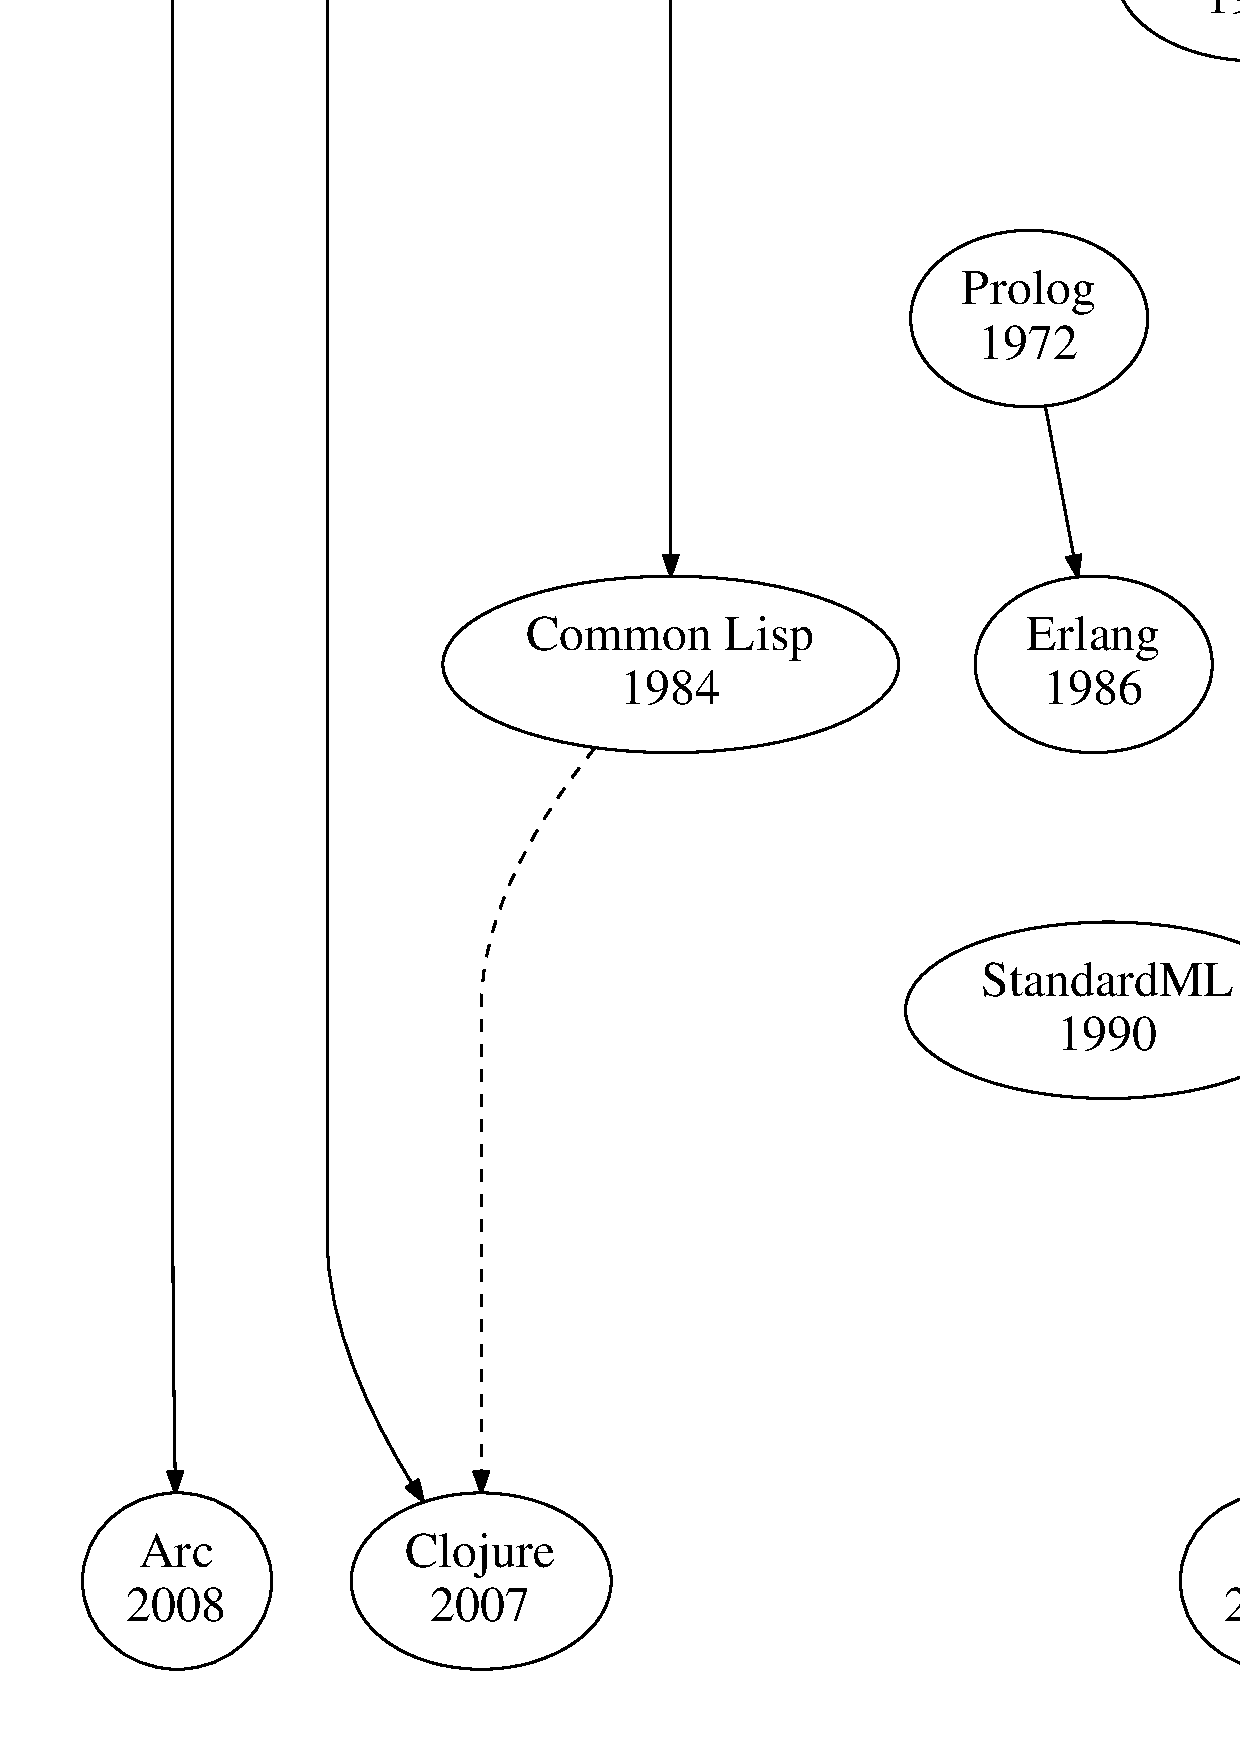
\includegraphics[width=\textwidth]{languages.pdf}
  \else
    \includegraphics[width=\textwidth]{languages.ps}
  \fi
\caption{Родословное древо функциональных языков}
\label{lineage}
\end{figure}

Как уже упоминалось в разделе \ref{benefits}, функциональные языки существуют довольно давно. Первый из них, Лисп, создан в 1958 году, всего на год позже первого императивного языка~--- Фортрана. Ещё один известный функциональный язык, РЕФАЛ, создан В.Ф.Турчиным в 1966 году. Но если РЕФАЛ стал широко известен довольно поздно (возможно, по причинам, далёким от программирования: он был создан в СССР в эпоху Холодной войны, а ФП развивалось в то время в основном по другую сторону Железного занавеса), то распространение Лиспа продолжалось всё время его существования. Уже в двухтысячных годах появились два новых популярных диалекта этого языка: Arc и Clojure.

Наиболее известные диалекты Лиспа~--- Common Lisp и Scheme. Первый чаще других вариантов Лиспа применяется на практике, а вторая используется в основном для обучения программированию. К сожалению, непоследовательная политика стандартизации сильно замедлила распространение Scheme как языка практического программирования.

Изучение Лиспа (скорее всего, Scheme) практически неизбежно для человека, интересущегося функциональным программированием, так как многие важные работы на эту тему используют именно Scheme в качестве языка примеров. Среди возможностей Scheme, отсутствующих в Эрланге, особенно интересны  продолжения (continuations)~--- способ сохранять как значение состояние программы в определённый момент.

Второй после Лиспа по влиятельности и многочисленности <<потомства>> функциональный язык это ML. В нём впервые была реализована очень мощная техника~--- {\em вывод типов}, то есть автоматическое определение компилятором типа выражения по контексту, в котором оно используется. Вывод типов избавляет программиста от целого класса неприятных ошибок. В этой книжке я использовал язык без вывода типов\footnote{На самом деле, похожие инструменты для Эрланга реализованы, но они гораздо слабее своих аналогов из языков-потомков ML.} только потому, что это сильно усложнило и удлинило бы курс.

Наиболее известные потомки ML это OCaml, F\# (построенный на базе OCaml язык для платформы .Net) и Haskell.

Именно Haskell считается <<передним краем>> исследований в области функционального программирования. В практическом программировании он применяется не так часто, возможно, потому, что его авторы очень жёстко отказываются вносить в язык полезные для индустрии, но <<некрасивые>> с точки зрения теории возможности~--- полушутливый девиз Haskell это <<Avoid success at all costs>> (<<Избегать успеха любой ценой>>). Пожалуй, Haskell~--- это второй после Scheme язык, изучения которого интересующемуся ФП человеку вряд ли удастся избежать. Изучить этот язык стоит хотя бы для того, чтобы познакомиться с такими интереснейшими концепциями, как ленивые вычисления или монады.

К сожалению, малопопулярен другой замечательный диалект ML~--- StandardML, очень красивый, гораздо более компактный, чем Haskell (и, на мой взгляд, более логичный синтаксически, чем OCaml и F\#) язык.

Ну и, наконец, не надо забывать, что Эрланг мы тоже изучили не до конца. Если вам понравился Эрланг, стоит всерьёз заняться изучением его возможностей. На самом деле, в этом курсе вообще не используется одно из главных преимуществ Эрланга~--- библиотека OTP, Open Telecom Platform, предоставляющая готовые решения для задач параллельного и распределённого программирования. <<За кадром>> остались также поведения (behaviours), обработка исключительных ситуаций, макросы и многое другое.

\section{Что ещё можно почитать про ФП}

Функциональному программированию посвящено довольно много книг, ресурсов в Интернете и журналов. Хорошей стартовой точкой для дальнейшего знакомства с миром ФП может стать журнал <<Практика функционального программирования>>, свободно доступный на сайте \url{http://fprog.ru/}. Кстати, в первом номере журнала опубликован обзор литературы по функциональному программированию, сделанный Алексеем Оттом~\cite{PFP_Ott}.

Ещё одна хорошая обзорная статья~--- <<Функциональное программирование для всех>> В.Ахмечета~\cite{Akhmechet}, опубликованная в журнале RSDN Magazine.

Среди книг прежде всего надо упомянуть <<Структуру и интерпретацию компьютерных программ>> Х.Абельсона и Дж.Сассмана~\cite{SICP}, которая по праву считается классической. Это учебник по программированию вообще, не только функциональному, но значительная часть материала изложена именно с помощью функциональных решений.

Большинство работ по алгоритмам и структурам данных расчитано на императивные языки. Эту ситуацию пытается исправить Крис Окасаки, автор книги <<Чисто функциональные структуры данных>>~\cite{Okasaki}. Ещё одна серьёзная работа по теоретическим аспектам программирования, ориентированная на ФП~--- <<Типы в языках программирования>> Б.Пирса~\cite{Pierce}.

Очень хороший пример практического программирования на функциональных языках приводится в статье Д.Астапова <<Давно не брал я в руки шашек>>~\cite{PFP_Astapov}. Интересующимся продвинутыми программистскими техниками будет, вероятно, интересно прочитать статьи А.Вознюка о продолжениях~\cite{PFP_Voznyuk} и И.Ключникова о суперкомпиляции~\cite{PFP_Klyuchnikov}. Впрочем, как уже говорилось, журнал <<Практика функционального программирования>>, в котором опубликованы все эти статьи, вообще рекомендуется к ознакомлению при наличии интереса к теме.

Замечательные учебники по языку Scheme и функциональному программированию~--- книги <<Little Schemer>>~\cite{little_schemer} и <<Seasoned Schemer>>~\cite{seasoned_schemer}, к сожалению, в отличие от SICP не переведены на русский язык.

Хороший вводный материал по языку Haskell~--- цикл статей Алексея Бешенова~\cite{Beshenov} и книга <<Изучай Haskell во имя добра!>>~\cite{Lipovacha}, а если говорить об источниках на английском языке~--- <<Real World Haskell>>~\cite{real_world_haskell}. По Стандартному ML на русском издана книга Р.Харпера <<Введение в Стандартный ML>>~\cite{Harper}.

Про возможности OTP, концепцию <<поведений>> (behaviours) можно прочитать в книге \cite{cesarini}. Из важных книг по Эрлангу, пока не переведённых на русский язык, надо упомянуть учебник Дж.Армстронга (создателя языка)~\cite{armstrong} и книгу <<Erlang and OTP in action>>~\cite{OTP_in_action}. Хороший вводный курс, правда, во многом дублирующий уже изложенное здесь~--- <<Learn You Some Erlang for Great Good>>~\cite{LYSE}.

\chapter*{Решения задач}
\addcontentsline{toc}{chapter}{Решения задач}
\markboth{Решения задач}{Азбука ФП}

\section*{Азбука ФП}
\addcontentsline{toc}{section}{Азбука ФП}

\solution{nand}

\lstinputlisting{abc/nand/logic.erl}

Вообще говоря, функцию \lstinline{nand} можно было бы определить гораздо проще:

\begin{lstlisting}
nand(true, true) -> false;
nand(_, _) -> true.
\end{lstlisting}

Но этот вариант функции \lstinline{nand} не будет выдавать ошибку, если передать ему в качестве аргументов что-то помимо атомов\index{Атом} \lstinline{true} и \lstinline{false}, что может затруднить поиск источника проблемы в неправильно написанной программе. Поэтому лучше перечислить все корректные варианты аргументов явно.

Помните, в Эрланге принят подход <<Let it fail>>~--- <<Пусть падает>>.

\solution{myor}

\lstinputlisting{abc/logic.erl}

\solution{author}

\lstinputlisting{abc/author.erl}

\solution{sign}

\lstinputlisting{abc/sign.erl}

\solution{divisor}

\lstinputlisting{abc/divisor.erl}

\solution{summ}

\lstinputlisting{abc/summ.erl}

\solution{divisors}

\lstinputlisting{abc/divisors.erl}

\solution{remainder}

\lstinputlisting{abc/remainder.erl}

\solution{number_sequence}

\lstinputlisting{abc/number_input.erl}

Эту задачу можно решить и иначе~--- например, вот так:

\lstinputlisting{abc/number_input/number_input.erl}

Идея решения та же самая, а как её оформить~--- вопрос вкуса. В таком варианте приодится дублировать оператор ввода, зато вместо \lstinline{case} используется сопоставление с образцом\index{Сопоставление с образцом}, что, по идее, должно делать код более понятным.

\solution{rember}

\lstinputlisting{abc/rember.erl}

\solution{listrev}

\lstinputlisting{abc/listrev.erl}

\solution{slice}

\lstinputlisting[language=erlang]{sugar/slice.erl}

\solution{flatten}

Алгоритм решения этой задачи можно коротко описать так: мы создаём временный список для хранения текущего разбираемого элемента (второй аргумент функции \lstinline{flatten/2}). Поначалу он пуст (это тот второй аргумент, который передаёт функции \lstinline{flatten/2} функция \lstinline{flatten/1}).

Если исходный список тоже пуст, то работа закончена (первый вариант функции).

Если исходный список не пуст, то мы берём его голову и помещаем во временный список для разбора (второе тело функции).

Если текущий разбираемый элемент это тоже список, то мы берём его голову, а хвост возвращаем в исходный список, где он будет дожидаться своей очереди (третье тело функции).

Наконец, если ни одно из предыдущих сопоставлений с образцом\index{Сопоставление с образцом} не увенчалось успехом, надо полагать, что хранилище разбираемых элементов не пусто (иначе бы сработали бы образцы 1 или 2) и то, что в нём лежит~--- не список (иначе сработал бы образец 3). Следовательно, это одиночное значение и мы можем смело помещать его в голову итогового списка.

\lstinputlisting{abc/flatten.erl}

\solution{palindrome}

\lstinputlisting[language=erlang]{best_practices/palindrome.erl}

\solution{perfect}
Функция \lstinline{divisors}, составляющая список делителей числа $N$, лежащих в интервале от 1 до $M$ включительно~--- это попросту индуктивное определение такого списка: если он заканчивается единицей, то только единица в него и войдёт, а если он должен состоять из чисел в интервале от единицы до некоего числа $M$, большего, чем единица, то в него войдут делители числа $N$ в интервале от 1 до $M-1$, а также само $M$, если оно тоже является делителем $N$.

Случай с единицей мы обрабатываем в \lstinline{divisors/1}, чтобы избежать лишнего вызова функции.

Функция \lstinline{lists:sum} из модуля \lstinline{lists}, подсчитывающая сумму списка чисел, ощутимо упрощает решение этой задачи.

Обратите внимание, что функция \lstinline{divisors} небезопасна и будет зацикливаться при значениях $M$ меньше 1. Здесь было разумным пожертвовать безопасностью в ущерб ясности; в реальных программах часто полезно делать наоборот.
\lstinputlisting[language=erlang]{abc/perfect.erl}
\pagebreak

\solution{brackets}
В этой задаче можно представлять строку для разбора либо как обычный эрланговский список, либо как битовую строку. Решение с битовыми строками чуть более громоздко, но в реальной жизни битовые строки гораздо полезнее <<строк>>, хранящихся как списки ASCII-кодов.

Алгоритм же в обоих решениях~--- один и тот же: сделаем стек, в который будем класть все открывающие скобки. Встречая закрывающую скобку, будем выпихивать со стека верхнее значение. Если тип закрывающей скобки из текущей позиции строки и открывающей скобки с вершины стека не совпали (или стек пуст), порядок скобок неправильный. Если после того, как вся строка разобрана, в стеке что-то осталось, порядок скобок тоже неправильный. Если же нам удалось подойти к концу строки с пустым стеком (или строка просто пустая), значит, порядок скобок~--- правильный.

\begin{figure}[!t,bracketspic]
\centerline{
\begin{pspicture}%[showgrid=true]
(10, 11)
\rput(2, 10.5){Входной список}
\rput(6.8, 10.5) {Стек}
\rput(0, 9){
  % Входной список
  \psgrid[gridlabels=0.0pt,subgriddiv=1](0,0)(0,0)(5,1)
  \rput(0.5, 0.5){[}
  \rput(1.5, 0.5){(}
  \rput(2.5, 0.5){<}
  \rput(3.5, 0.5){)}
  \rput(4.5, 0.5){]}
  % Операция
  \psbezier{->}(0.5,0)(0.5,-1)(6.5,0)(6.5,-1)
}
\rput(0, 7) {
  % Входной список
  \psgrid[gridlabels=0.0pt,subgriddiv=1](0,0)(0,0)(4,1)
  \rput(0.5, 0.5){(}
  \rput(1.5, 0.5){<}
  \rput(2.5, 0.5){)}
  \rput(3.5, 0.5){]}
  % Операция
  \psbezier{->}(0.5,0)(0.5,-1)(6.5,0)(6.5,-1)
  % Стек
  \psgrid[gridlabels=0.0pt,subgriddiv=1](0,0)(6,0)(7,1)
  \rput(6.5, 0.5){(}
}
\rput(0, 5) {
  % Входной список
  \psgrid[gridlabels=0.0pt,subgriddiv=1](0,0)(0,0)(3,1)
  \rput(0.5, 0.5){<}
  \rput(1.5, 0.5){)}
  \rput(2.5, 0.5){]}
  % Операция
  \psbezier{->}(0.5,0)(0.5,-1)(6.5,0)(6.5,-1)
  % Стек
  \psgrid[gridlabels=0.0pt,subgriddiv=1](0,0)(6,0)(8,1)
  \rput(6.5, 0.5){(}
  \rput(7.5, 0.5){[}
}
\rput(0, 3) {
  % Входной список
  \psgrid[gridlabels=0.0pt,subgriddiv=1](0,0)(0,0)(2,1)
  \rput(0.5, 0.5){)}
  \rput(1.5, 0.5){]}
  % Операция
  \psbezier{->}(0.5,0.0)(0.5,-1)(0.5,-1)(3.5,-1)
  \psbezier{->}(6.5,0.0)(6.5,-1)(6.5,-1)(4.5,-1)
  \rput(4, -1){\pscirclebox{?}}
  \psline{->}(4,-1.5)(4,-2)
  % Стек
  \psgrid[gridlabels=0.0pt,subgriddiv=1](0,0)(6,0)(9,1)
  \rput(6.5, 0.5){<}
  \rput(7.5, 0.5){(}
  \rput(8.5, 0.5){[}
  % Возвращаемое значение
  \rput(4, -2.5){false}
  \psbezier{->}(4.75,-2.5)(5.5,-3)(5.5,-2)(6.25,-2.5)
  \rput(7, -2.5){false}
}
\end{pspicture}
}
\caption{Функция \lstinline{is_valid_string/2} проверяет скобочную структуру <<[(<)]>> на правильность. Слева~--- входной список (первый аргумент функции), справа~--- стек (второй аргумент функции).}
\label{bracketspic}
\end{figure}

\lstinputlisting[language=erlang]{abc/brackets_str.erl}
\pagebreak
\lstinputlisting[language=erlang]{abc/brackets.erl}
\pagebreak

\solution{queue}

Идея решения вот в чём: реализуем очередь как два списка, входной и выходной. При помещении значения в очередь будем добавлять его в голову входного списка. При извлечении значения из очереди проверим, пуст ли выходной список. Если да, проверим, пуст ли входной. Если пуст и он, очередь пуста (второй вариант тела функции). А если входной список не пуст, развернём его, отдадим голову получившегося списка как выходное значение, а хвост поместим в выходной список (входной список, соответственно, становится пустым). Эти действия описаны в первом варианте тела функции. Ну а если выходной список не пуст, просто отдаём его голову, т.к. значения в нём уже стоят в правильном порядке (третий вариант тела функции).

Работа с организованной таким образом очередью будет выглядеть примерно так.

\begin{figure}[!t,queuepic]
\centerline{
\begin{pspicture}%[showgrid=true]
(9, 21)
\rput(3.0, 20.5){Входной}
\rput(3.0, 19.5){список}
\rput(6.0, 20.5){Выходной}
\rput(6.0, 19.5){список}
\rput(0, 18) {
  \psframe[linestyle=dotted](1.8,-0.2)(7.2, 1.2)
  % Операция
  \rput(0.5, 0.5){1}
  \psline{->}(0.8, 0.5)(1.6, 0.5)
}
\rput(0, 16) {
  \psframe[linestyle=dotted](1.8,-0.2)(7.2, 1.2)
  % Входной список
  \psgrid[gridlabels=0.0pt,subgriddiv=1](0,0)(2,0)(3,1)
  \rput(2.5, 0.5){1}
  % Операция
  \rput(0.5, 0.5){2}
  \psline{->}(0.8, 0.5)(1.6, 0.5)
}
\rput(0, 14) {
  \psframe[linestyle=dotted](1.8,-0.2)(7.2, 1.2)
  % Входной список
  \psgrid[gridlabels=0.0pt,subgriddiv=1](0,0)(2,0)(4,1)
  \rput(2.5, 0.5){2}
  \rput(3.5, 0.5){1}
  % Операция
  \rput(0.5, 0.5){3}
  \psline{->}(0.8, 0.5)(1.6, 0.5)
}
\rput(0, 12) {
  \psframe[linestyle=dotted](1.8,-0.2)(7.2, 1.2)
  % Операция
  \rput(8.5, 0.5){1}
  \psline{->}(7.4, 0.5)(8.2, 0.5)
  % Выходной список
  \psgrid[gridlabels=0.0pt,subgriddiv=1](0,0)(5,0)(7,1)
  \rput(5.5, 0.5){3}
  \rput(6.5, 0.5){2}
}
\rput(0, 10) {
  \psframe[linestyle=dotted](1.8,-0.2)(7.2, 1.2)
  % Операция
  \rput(0.5, 0.5){4}
  \psline{->}(0.8, 0.5)(1.6, 0.5)
  % Выходной список
  \psgrid[gridlabels=0.0pt,subgriddiv=1](0,0)(5,0)(7,1)
  \rput(5.5, 0.5){3}
  \rput(6.5, 0.5){2}
}
\rput(0, 8) {
  \psframe[linestyle=dotted](1.8,-0.2)(7.2, 1.2)
  % Входной список
  \psgrid[gridlabels=0.0pt,subgriddiv=1](0,0)(2,0)(3,1)
  \rput(2.5, 0.5){4}
  % Операция
  \rput(0.5, 0.5){5}
  \psline{->}(0.8, 0.5)(1.6, 0.5)
  % Выходной список
  \psgrid[gridlabels=0.0pt,subgriddiv=1](0,0)(5,0)(7,1)
  \rput(5.5, 0.5){3}
  \rput(6.5, 0.5){2}
}
\rput(0, 6) {
  \psframe[linestyle=dotted](1.8,-0.2)(7.2, 1.2)
  % Входной список
  \psgrid[gridlabels=0.0pt,subgriddiv=1](0,0)(2,0)(4,1)
  \rput(2.5, 0.5){5}
  \rput(3.5, 0.5){4}
  % Операция
  \rput(8.5, 0.5){2}
  \psline{->}(7.4, 0.5)(8.2, 0.5)
  % Выходной список
  \psgrid[gridlabels=0.0pt,subgriddiv=1](0,0)(6,0)(7,1)
  \rput(6.5, 0.5){3}
}
\rput(0, 4) {
  \psframe[linestyle=dotted](1.8,-0.2)(7.2, 1.2)
  % Входной список
  \psgrid[gridlabels=0.0pt,subgriddiv=1](0,0)(2,0)(4,1)
  \rput(2.5, 0.5){5}
  \rput(3.5, 0.5){4}
  % Операция
  \rput(8.5, 0.5){3}
  \psline{->}(7.4, 0.5)(8.2, 0.5)
}
\rput(0, 2) {
  \psframe[linestyle=dotted](1.8,-0.2)(7.2, 1.2)
  % Операция
  \rput(8.5, 0.5){4}
  \psline{->}(7.4, 0.5)(8.2, 0.5)
  % Выходной список
  \psgrid[gridlabels=0.0pt,subgriddiv=1](0,0)(6,0)(7,1)
  \rput(6.5, 0.5){5}
}
\rput(0, 0) {
  \psframe[linestyle=dotted](1.8,-0.2)(7.2, 1.2)
  % Операция
  \rput(8.5, 0.5){5}
  \psline{->}(7.4, 0.5)(8.2, 0.5)
}
\end{pspicture}
}
\caption{Организация очереди из двух списков.}
\label{queuepic}
\end{figure}

Компилируем модуль, загружаем определение записи:
\erlshell{c(listqueue).}{\{ok,listqueue\}}
\erlshell{rr("queue.hrl").}{{[}queue{]}}

Создаём новую очередь:
\erlshell{Q1 = \#queue\{\}.}{\#queue\{in = [],out = []\}}

Помещаем в очередь значение 1:
\erlshell{Q2 = listqueue:enqueue(Q1, 1).}{\#queue\{in = [1],out = []\}}

Помещаем в очередь значение 2:
\erlshell{Q3 = listqueue:enqueue(Q2, 2).}{\#queue\{in = [2,1],out = []\}}

Помещаем в очередь значение 3:
\erlshell{Q4 = listqueue:enqueue(Q3, 3).}{\#queue\{in = [3,2,1],out = []\}}

Извлекаем из очереди первое значение (1)~--- в этот момент входной список будет развёрнут и перемещён в выходной:
\erlshell{\{ok, Out1, Q5\} = listqueue:dequeue(Q4).}{\{ok,1,\#queue\{in = [],out = [2,3]\}\}}
\erlshell{Out1.}{1}

Добавляем в очередь значение 4 (с этого момента формируется новый входной список):
\erlshell{Q6 = listqueue:enqueue(Q5, 4).}{\#queue\{in = [4],out = [2,3]\}}

Добавляем в очередь значение 5:
\erlshell{Q7 = listqueue:enqueue(Q6, 5).}{\#queue\{in = [5,4],out = [2,3]\}}

Извлекаем из очереди второе значение (2):
\erlshell{\{ok, Out2, Q8\} = listqueue:dequeue(Q7).}{\{ok,2,\#queue\{in = [5,4],out = [3]\}\}}

Извлекаем из очереди третье значение (3):
\erlshell{\{ok, Out3, Q9\} = listqueue:dequeue(Q8).}{\{ok,3,\#queue\{in = [5,4],out = []\}\}}

Извлекаем из очереди четвёртое значение (4)~--- выходной список пуст, снова разворачиваем входной список и перемещаем его на место опустевшего выходного:
\erlshell{\{ok, Out4, Q10\} = listqueue:dequeue(Q9).}{\{ok,4,\#queue\{in = [],out = [5]\}\}}

Извлекаем из очереди пятое значение (5):
\erlshell{\{ok, Out5, Q11\} = listqueue:dequeue(Q10).}{\{ok,5,\#queue\{in = [],out = []\}\}}

Очередь пуста, при попытке извлечения дальнейших значений будет возвращена информация об ошибке:
\erlshell{listqueue:dequeue(Q11).}{\{error,"Queue is empty"\}}

Несмотря на наличие в этом алгоритме <<тяжёлой>> операции разворачивания списка, требующей $N$ шагов для списка из $N$ элементов, условиям задачи он отвечает, т.к. каждый проходящий через очередь элемент участвует в этой операции только один раз.

\lstinputlisting[language=erlang]{abc/listqueue.erl}

\solution{node_cut}

Обратите внимание на то, как функции \lstinline{trim/2} и \lstinline{trim/3} рекурсивно вызывают друг друга. Это полезный приём, который позволяет упростить отладку и тестирование, а также улучшить читаемость кода за счёт избавления от громоздких операторов ветвления.

\lstinputlisting[language=erlang]{abc/trimtree.erl}

\solution{node_count}

\lstinputlisting[language=erlang]{abc/treemeter.erl}

\section*{Полезные приёмы}
\addcontentsline{toc}{section}{Полезные приёмы}
\markright{Полезные приёмы}

\solution{already}

Хвостовая рекурсия уже используется в решениях задач \ref{summ}, \ref{divisors}, \ref{remainder}, \ref{listrev}, \ref{brackets}.

\solution{tail}

Функцию \lstinline{rember/2} из задачи \ref{rember} можно переписать следующим образом:

\lstinputlisting[language=erlang]{abc/tailrember.erl}

Проблема в том, что такой способ обработки списка разворачивает его, и нам приходится вызывать \lstinline{lists:reverse}, чтобы вернуть исходный порядок следования элементов. Поэтому применение здесь хвостовой рекурсии не очень оправдано. В решениях других задач применение хвостовой рекурсии принесёт ещё больше сложностей.

Не надо применять хвостовую рекурсию по любому поводу. Во-первых, она не всегда эффективнее обычной, во-вторых, помните: сначала стабильная работа программы, потом оптимизация.

\solution{perfect_list}

\lstinputlisting[language=erlang]{best_practices/perfect.erl}
\pagebreak

\solution{maptree}

\lstinputlisting[language=erlang]{best_practices/maptree.erl}

\solution{length}
\begin{lstlisting}
lists:foldl(fun(_, Length) -> Length + 1 end, 0, L).
\end{lstlisting}

\solution{foldrev}

\lstinputlisting[language=erlang]{best_practices/foldrev.erl}

\solution{mean}

\lstinputlisting[language=erlang]{best_practices/mean.erl}

\solution{foldl1}

\lstinputlisting[language=erlang]{best_practices/mylists.erl}

\solution{foldseq}

\lstinputlisting[language=erlang]{best_practices/myseq.erl}

\solution{ismemberof}

\lstinputlisting[language=erlang]{best_practices/ismemberof.erl}

\section*{Приятные мелочи}
\addcontentsline{toc}{section}{Приятные мелочи}
\markright{Приятные мелочи}

\solution{short_perfect}

\lstinputlisting[language=erlang]{sugar/perfect.erl}

\solution{common}

\lstinputlisting[language=erlang]{sugar/common_members.erl}

\solution{multiplication}

\lstinputlisting[language=erlang]{best_practices/multiplication.erl}

\solution{common_without_member}

\lstinputlisting[language=erlang]{sugar/common2.erl}

\solution{queens}

\lstinputlisting[language=erlang]{sugar/queens.erl}

%% Решение из статьи про задачу в Википедии %% (http://ru.wikipedia.org/wiki/%D0%97%D0%B0%D0%B4%D0%B0%D1%87%D0%B0_%D0%BE_%D0%B2%D0%BE%D1%81%D1%8C%D0%BC%D0%B8_%D1%84%D0%B5%D1%80%D0%B7%D1%8F%D1%85#.D0.A0.D0.B5.D0.B0.D0.BB.D0.B8.D0.B7.D0.B0.D1.86.D0.B8.D1.8F_.D0.BD.D0.B0_Erlang):

%% pmut([])->
%%         [[]];
%% pmut(A) ->
%%         [[H|T] || H <- A, T <- pmut(A--[H])].
 
%% start() ->
%%         N = 8, % size of board / num of queens (N>=4)
%%         ListP = pmut(lists:seq(1,N)),
%%         [Q || Q <- ListP, length(lists:usort([lists:nth(X,Q)+X || X <- %% Q])) == N, 
%%         length(lists:usort([lists:nth(X,Q)-X || X <- Q])) == N]

\solution{foldrrev}

\lstinputlisting[language=erlang]{sugar/foldrrev.erl}

\solution{linearize}

\lstinputlisting[language=erlang]{sugar/trees-linearize/trees.erl}

\solution{hanoi}

Сформулируем принципы перекладывания стопки из $N$ дисков.

Базовый случай в этой задаче~--- $N=0$, т.е. ситуация, когда нам ничего перекладывать не нужно. Большее количество дисков перекладывается по следующему алгоритму (стержень, с которого перемещаем диски, будем называть исходным, стержень, на который перемещаем диски~--- целевым, а третий~--- вспомогательным):

\begin{enumerate}
\item Взять $N-1$ дисков и переместить их с исходного стержня на вспомогательный.
\item Переместить оставшийся на исходном стержне диск на целевой стержень.
\item Переместить $N-1$ дисков со вспомогательного стержня на целевой.
\end{enumerate}

Первый и третий шаги предполагают перекладывание стопки дисков, то есть рекурсивный вызов процедуры перекладывания. Но так как в каждом следующем вызове $N$ гарантированно уменьшается, мы можем быть уверены, что рано или поздно рекурсия закончится.

\lstinputlisting[language=erlang]{sugar/hanoi.erl}

\solution{dropwhile}

Сложность с реализацией \lstinline{dropwhile} в том, что реакция на элемент, для которого переданная функция возвращает \lstinline{true}, должна отличаться в зависимости от того, встретился ли нам уже элемент, для которого эта функция вернула \lstinline{false}. Так как мы имеем дело со свёрткой\index{Свёртка списка}, мы не можем ввести какой-то дополнительный параметр, указывающий, так ли это~--- ведь тогда свёртка вернёт его вместе с итоговым списком, а это не то, что нам нужно.

Но на самом деле при левой свёртке\index{Свёртка списка!левая} таким параметром является сам итоговый список: если он пуст, значит, не отвечающий критерию элемент нам ещё не встречался и мы должны проверить текущий элемент с помощью функции-аргумента. Если список не пуст, мы должны безо всяких проверок поместить в него текущий элемент.

\lstinputlisting[language=erlang]{best_practices/dropwhile.erl}

Реализовать \lstinline{dropwhile} с помощью правой свёртки\index{Свёртка списка!правая}, строго говоря, невозможно~--- правая свёртка начинается с конца списка, что не позволяет нам найти первое с начала списка вхождение элемента с её помощью. Но динамическая типизация Эрланга позволяет нам реализовать обходное решение, жульническое по сути (реальная работа делается вне свёртки), но позволяющее <<обмануть>> функцию \lstinline{foldr}, подсунув ей функцию, которая формально удовлетворяет условиям задачи:

\lstinputlisting[language=erlang]{best_practices/rdropwhile.erl}

Идея этого решения в следующем: мы заранее находим первый элемент в списке, для которого функция \lstinline{F} вернёт \lstinline{false} и запоминаем его позицию (далее будем называть её <<линией отреза>>. После этого мы определяем функцию \lstinline{Trim}, у которой есть два варианта списка аргументов: либо текущий элемент списка и кортеж вида {\em \{Накопленный хвост списка, Позиция текущего элемента, Линия отреза\}}, либо текущий элемент и список.

\lstinline{Trim} будет добавлять к накопленному хвосту списка элемент за элементом, пока позиция текущего элемента не совпадёт с линией отреза. В этот момент она оставит в аргументе-накопителе только список. Следующие вызовы, обнаружив во втором аргументе список вместо кортежа, просто передадут аргумент-накопитель дальше.

Обратите внимание, что ситуация, когда элемент, для которого \lstinline{F} возвращает \lstinline{false}, так и не был найден, требует особой обработки.

Надо ещё раз подчеркнуть, что это решение является хаком в самом плохом смысле этого слова и непереносимо на многие функциональные языки с более строгим контролем типов, вроде Стандартного ML и Haskell (решения, построенные на аналогичной идее, пожалуй, возможны и там, но ценой ещё более уродливых ухищрений).

\solution{permutations}

Идея решения этой задачи вот в чём. В список перестановок списка длины $1$ входит единственный элемент~--- он сам. А перестановки списка большей длины можно получить так: по очереди удалять из списка каждый элемент, получать все перестановки оставшихся и в начало каждой из них подставлять удалённый элемент.

% Я видел где-то лучшее решение с --

\lstinputlisting[language=erlang]{sugar/permutations.erl}

\section*{От функционального программирования к параллельному}
\addcontentsline{toc}{section}{От функционального программирования к параллельному}
\markright{От ФП к ПП}

\solution{approximation}

\lstinputlisting[language=erlang]{parallel/montecarlo.erl}

\solution{fibmem}

\lstinputlisting[language=erlang]{parallel/fibmem.erl}

% Приложение: отладчик, запускающийся по debugger:start()? Трассировщик, если он может быть чем-то полезен? EUnit?

% Приложение: установка Эрланга на разных платформах?

\addcontentsline{toc}{chapter}{Литература}
\begin{thebibliography}{99}
\bibitem[Абельсон 2010]{SICP}
Абельсон Х., Сассман Дж. Дж. Структура и интерпретация компьютерных программ. М.: <<Добросвет>>, <<КДУ>>, 2010.
\bibitem[Астапов 2009]{PFP_Astapov}
Астапов Д. Давно не брал я в руки шашек // Практика функционального программирования, №1, 2009.
\bibitem[Ахмечет 2006]{Akhmechet}
Ахмечет В. Функциональное программирование для всех. // RSDN Magazine, №2, 2006.
\bibitem[Бешенов 2010]{Beshenov}
Бешенов А. Функциональное программирование на Haskell.\\
\href{http://www.ibm.com/developerworks/ru/library/l-haskell/}{Часть 1. Введение.}\\
\href{http://www.ibm.com/developerworks/ru/library/l-haskell2/}{Часть 2.Основные типы и классы.}\\
\href{http://www.ibm.com/developerworks/ru/library/l-haskell3/}{Часть 3. Определение функций.}\\
\href{http://www.ibm.com/developerworks/ru/library/l-haskell4/}{Часть 4. Свертки списков.}
\bibitem[Вознюк 2011]{PFP_Voznyuk}
Вознюк А. Продолжения в практике. // Практика функционального программирования, №7, 2011.
\bibitem[Златопольский 2007]{zlatopolsky}
Златопольский Д.М. Программирование: типовые задачи, алгоритмы, методы. М., 2007.
\bibitem[Ключников 2011]{PFP_Klyuchnikov}
Ключников И. Суперкомпиляция: идеи и методы. // Практика функционального программирования, №7, 2011.
\bibitem[Липовача 2012]{Lipovacha}
Липовача М. Изучай Haskell во имя добра! М.: <<ДМК Пресс>>, 2012.
\bibitem[Отт 2009]{PFP_Ott}
Отт А. Обзор литературы о функциональном программировании. // Практика функционального программирования, №1, 2009.
\bibitem[Пирс 2012]{Pierce}
Пирс Б., Типы в языках программирования. М.: <<Лямбда пресс>>, <<Добросвет>>, 2012.
\bibitem[Харпер 1996]{Harper}
Харпер Р. Введение в Стандартный ML. М., 1996.
\bibitem[Чезарини 2012]{cesarini}
Чезарини Ф., Томпсон С. Программирование в Эрланг. М.: <<ДМК Пресс>>,
2012.
\bibitem[Шень 2004]{shen}
Шень А. Программирование: теоремы и задачи. М.: МЦНМО, 2004.
\bibitem[99 problems]{99problems}
99 Problems на выбранном языке (точно есть для \href{http://www.haskell.org/haskellwiki/99_questions}{Haskell}, \href{http://aperiodic.net/phil/scala/s-99/}{Scala}, \href{https://sites.google.com/site/prologsite/prolog-problems}{Prolog}, \href{http://www.christiankissig.de/cms/index.php/en/programming/28-ocaml/28-99-problems-in-ocaml}{OCaml}, \href{http://www.informatimago.com/develop/lisp/l99/index.html}{Common Lisp}).
\bibitem[Armstrong 2007]{armstrong}
Armstrong J. Programming Erlang: Software for a Concurrent World. Pragmatic Bookshelf, 2007.
\bibitem[Friedman 1996]{little_schemer}
Friedman D.P., Fellsen M. The Little Schemer. MIT Press, 1996.
\bibitem[Friedman 1996,2]{seasoned_schemer}
Friedman D.P., Fellsen M. The Seasoned Schemer. MIT Press, 1996.
\bibitem[LYSE]{LYSE}
Learn You Some Erlang for Great Good, \url{http://learnyousomeerlang.com/}.
\bibitem[Logan 2011]{OTP_in_action}
Logan M., Merritt E., Carlsson R. Erlang and OTP in action. Manning Publications, 2011.
\bibitem[Miller]{miller}
Evan Miller. The Joy of Erlang; Or, How To Ride A Toruk, \url{http://www.evanmiller.org/joy-of-erlang.html}.
\bibitem[Okasaki 1999]{Okasaki}
Okasaki C. Purely Functional Data Structures. Cambridge University Press, 1999.
\bibitem[O'Sullivan 2008]{real_world_haskell}
O'Sullivan B., Goerzen J., D.B. Stewart. Real World Haskell. Code You Can Believe In. O'Reilly, 2008.
\end{thebibliography}

\appendix

\pagebreak
\addcontentsline{toc}{chapter}{Приложения}

\chapter{Краткий справочник по используемым функциям}

\section*{Ввод-вывод}
\addcontentsline{toc}{section}{Ввод-вывод}
\markright{Ввод-вывод}

Здесь приводятся только те функции, которые требуются для той или иной задачи. С полной документацией на упомянутые модули можно ознакомиться на сайте языка: \url{http://erlang.org/doc/}.

\begin{funcdescr}
\funcdoc{io:format/1}{Принимает строку с командами формата и выводит её на экран.}
\funcdoc{io:format/2}{Принимает строку с командами формата и список подставляемых значений; выводит на экран строку, в которую подставлены значения в соответствии с командами формата.}
\funcdoc{io:fread/2}{Принимает подсказку и строку формата; читает со стандартного ввода выражения и пытается привести их к типам, заданным строкой формата; в случае успеха возвращает кортеж из атома \lstinline{ok} и списка прочитанных значений, в случае  ошибки~--- кортеж из атома \lstinline{error} и описания ошибки.}
\funcdoc{io:read/1}{Принимает подсказку для ввода; читает со стандартного ввода выражение Эрланга и возвращает кортеж из атома \lstinline{ok} и прочитанного выражения в случае успеха либо кортеж из атома \lstinline{error} и описания ошибки в случае ошибки.}
\end{funcdescr}

\section*{Математика}
\addcontentsline{toc}{section}{Математика}
\markright{Математика}

\begin{funcdescr}
\funcdoc{abs/1}{Возвращает модуль числа.}
\funcdoc{math:sqrt/1}{Возвращает квадратный корень своего аргумента.}
\funcdoc{random:uniform/0}{Возвращает случайное вещественное число в интервале от 0.0 до 1.0.}
\funcdoc{random:uniform/1}{Возвращает случайное целое число в интервале от 1 до своего аргумента.}
\end{funcdescr}

\section*{Обработка списков}
\addcontentsline{toc}{section}{Обработка списков}
\markright{Обработка списков}

\begin{funcdescr}
\funcdoc{length/1}{Принимает список; возвращает длину этого списка.}
\funcdoc{lists:dropwhile/2}{Принимает функцию-тест и список; возвращает список, из которого выброшены все элементы до первого, для которого функция-тест вернула \lstinline{false}.}
\funcdoc{lists:filter/2}{Принимает функцию-тест и список; возвращает список, в котором оставлены только те элементы, для которых функция-тест вернула \lstinline{true}.}
\funcdoc{lists:foldl/3}{Левая свёртка: принимает функцию, начальное значение накопителя и список. Функция-аргумент должна принимать два параметра: текущее значение накопителя и текущий элемент списка, а возвращать новое значение накопителя. Применяет функцию-аргумент ко всем элементам списка слева направо (от первого до последнего). Возвращает итоговое значение накопителя.}
\funcdoc{lists:foldr/3}{Правая свёртка: принимает функцию, начальное значение накопителя и список. Функция-аргумент должна принимать два параметра: текущее значение накопителя и текущий элемент списка, а возвращать новое значение накопителя. Применяет функцию-аргумент ко всем элементам списка cправа налево (от последнего до первого). Возвращает итоговое значение накопителя.}
\funcdoc{lists:map/2}{Принимает функцию от одного аргумента и список; возвращает список результатов применения переданной функции к элементам списка.}
\funcdoc{lists:max/1}{Принимает список; возвращает самый большой элемент списка.}
\funcdoc{lists:member/2}{Принимает значение и список; возвращает \lstinline{true}, если значение содержится в списке, и \lstinline{false}, если нет.}
\funcdoc{lists:reverse/1}{Принимает список; возвращает список, элементы которого идут в обратном относительно исходного списка порядке.}
\funcdoc{lists:seq/2}{Принимает два целых числа; возвращает идущие подряд целые числа от первого до второго аргумента включительно.}
\funcdoc{lists:sort/1}{Принимает список; возвращает список с элементами исходного списка, отсортированными по возрастанию.}
\funcdoc{lists:sort/2}{Принимает функцию сравнения и список;   возвращает список, отсортированный по возрастанию в соответствии с функцией сравнения. Функция сравнения должна принимать два аргумента и возвращать \lstinline{true}, если первый аргумент меньше второго или равен ему, и \lstinline{false} в противном случае.}
\funcdoc{lists:sum/1}{Принимает список чисел; возвращает сумму его элементов.}
\end{funcdescr}

\section*{Структуры данных}
\addcontentsline{toc}{section}{Структуры данных}
\markright{Структуры данных}

\begin{funcdescr}
\funcdoc{dict:new/0}{Возвращает пустой словарь.}
\funcdoc{dict:append/3}{Принимает ключ, значение и словарь; возвращает новый словарь, в котором к значениям по переданному ключу добавилось переданное значение.}
\funcdoc{dict:find/2}{Принимает ключ и словарь. Если в словаре содержатся значения по этому ключу, возвращает кортеж \lstinline{\{ok, Values\}}, где \lstinline{Values}~--- список найденных значений; в противном случае возвращает атом \lstinline{error}.}
\end{funcdescr}

\section*{Служебные функции Эрланга}
\addcontentsline{toc}{section}{Служебные функции Эрланга}
\markright{Служебные функции Эрланга}

\begin{funcdescr}
\funcdoc{register/2}{Принимает атом и идентификатор процесса; если атом ещё не используется в качестве имени процесса, регистрирует процесс под этим именем и возвращает \lstinline{true}.}
\funcdoc{self/0}{Возвращает идентификатор процесса, из которого вызвана.}
\funcdoc{spawn/1}{Принимает функцию; запускает её в отдельном процессе и возвращает идентификатор этого процесса.}
\funcdoc{timer:tc/3}{Принимает имя модуля, имя функции и список аргументов; возвращает время в микросекундах, затраченное на вычисление переданной функции от переданных аргументов.}
\end{funcdescr}

\chapter{Команды формата}

\section*{Вывод}
\addcontentsline{toc}{section}{Вывод}
\markright{Вывод}

\renewcommand{\arraystretch}{1.5}
\begin{longtabu} to \linewidth {|X|X[2.8]|}
  \hline
  \lstinline{s} & Вывести строку.\\
  \hline
  \lstinline{w} & Вывести выражение Эрланга.\\
  \hline
  \lstinline{p} & Вывести выражение Эрланга с аккуратными переносами длинных строк и отступами. По умолчанию считает строку равной 80 символам. Принимает аргумент, задающий длину строки: так, команда формата <<{\tt \textasciitilde{}62p}>> будет считать длину строки равной 62 символам.\vspace{1ex}\\
  \hline
  \lstinline{B} & Вывести число в заданной системе счисления с основанием от 2 до 36, по умолчанию используется основание 10.\vspace{1ex}\\
  \hline
  \lstinline{n} & Перейти на новую строку.\\
  \hline
\end{longtabu}

\section*{Ввод}
\addcontentsline{toc}{section}{Ввод}
\markright{Ввод}

\begin{longtabu} to \linewidth {|X|X[2.8]|}
  \hline
  \lstinline{d} & Прочитать десятичное целое.\\
  \hline
  \lstinline{f} & Прочитать вещественное число.\\
  \hline
  \lstinline{s} & Прочитать строку. Принимает числовой аргумент~--- ограничение длины строки. Также принимает аргумент \lstinline{t}, включающий поддержку символов Unicode (нужно, если вы собираетесь вводить, например, русские буквы).\vspace{1ex}\\
  \hline
\end{longtabu}

Здесь приведены не все команды формата. Полное описание можно прочитать в документации модуля \lstinline{io} (\url{http://erlang.org/doc/man/io.html}).

% Предметный указатель
\pagebreak % Это хак, не знаю, как ещё его научить ставить правильную страницу.
\addcontentsline{toc}{chapter}{Предметный указатель}
\documentclass[
  paper=a4,
  fontsize=14pt,
  openany,
  appendixprefix=true
]{scrbook}
\usepackage{quicktour}
\author{Ю.А.Широков}
\title{Короткая экскурсия в функциональное программирование}
\begin{document}

\maketitle

\tableofcontents

\chapter*{От автора}
\addcontentsline{toc}{chapter}{От автора}
\markboth{От автора}{От автора}

Эта книга появилась практически случайно. Началось всё с разговоров о функциональном программировании с коллегами. В этих разговорах мне очень не хватало простых и понятных объяснений, в чём именно состоит функциональный подход. После нескольких таких бесед мне показалось, что я научился описывать функциональное программирование просто и при этом достаточно точно. Чтобы не забыть получившиеся формулировки, я решил записать их в виде короткого коспекта.

Конспект получился не таким уж коротким. Когда я его закончил, мне стало обидно, что несколько часов моего времени ушли на текст, который прочитаю только я сам. Поэтому, как только мне предоставился случай, я сказал нескольким знакомым, что с удовольствием бы прочитал вводную лекцию по функциональному программированию каким-нибудь студентам или продвинутым старшим школьникам.

Среди этих нескольких знакомых оказался Александр Трусевич, который предложил мне провести курс по функциональному программированию в физическом отделении Летней Экологической Школы (ЛЭШ). Не представляя себе, во что ввязываюсь, я согласился.

Быстро выяснилось, что конспект, которым я так гордился, никуда не годится~--- он полон непонятных школьникам терминов, зануден и слишком абстрактен. Пришлось писать с нуля новый рассказ о функциональном программировании (ставший в этой книге первой главой). Кроме того, пришлось заняться подбором задач. Эти-то задачи вместе с короткими объяснениями приёмов, применяемых для их решения, и стали в конце концов главным содержанием книги.

Сделать полноценный курс за лето 2012 года я не успел. Впрочем, и на ЛЭШ не попал. А к следующему лету курс увеличился насколько, что вываливать его весь на школьников ЛЭШ за пять дней было бы негуманно. И мне снова пришлось думать, в какой форме организовать свои заметки, чтобы работа не пропала зря.

Я хочу поблагодарить всех причастных к проведению ЛЭШ, её физического отделения и, конечно же, в особенности тех, кто слушал мой курс, а также героическую команду организаторов. Отдельное спасибо Александру Трусевичу, которому принадлежала сама исходная идея курса.

Разумеется, большинство приведённых в книге задач придумал не я. Все задачи, для которых удалось отыскать источник, снабжены ссылками на эти источники. Вклад авторов этих замечательных задач в книгу~--- никак не меньше моего.

Я вряд ли бы взялся оформить свои заметки в виде книги без вдохновляющего примера Георгия Бронникова, переведшего на русский язык три важнейших работы по функциональному программированию (\cite{SICP}, \cite{Pierce}, \cite{Okasaki}). Без книжки Сергея Львовского <<Набор и вёрстка в системе \LaTeX>> я не смог бы эти заметки оформить.

Анна Белякова, Татьяна Трошина и Алексей Туманов протестировали исходный набор задач и нашли в нём огромное количество опечаток, неточностей и ошибок. Кроме того, они указали мне множество плохо изложенных и непонятных мест в исходном варианте текста.

Последнее по порядку, но не по значению: моя жена, Катерина Шананина, проверила (и кое-где подправила) математические и околоматематические рассуждения, протестировала некоторые задачи и указала на множество неудачно сформулированных мест. Кроме того, именно она много лет назад убедила меня попробовать писать на языке LISP, познакомив с функциональным программированием.

Спасибо!

\chapter{Зачем нужно функциональное программирование}

\epigraph{Программы должны писаться для того,чтобы их читали люди, и только во вторую очередь для выполнения машиной.}{Х.Абельсон, Дж.Дж.Сассман}

\section{В погоне за ясностью}

Понимаем ли мы программы, которые пишем?

Если речь о маленьких программах, решающих не слишком сложные задачи, то обычно понимаем, конечно. Чтобы сделать непонятной простую программу, надо специально постараться. Кстати, некоторые и стараются~--- есть даже специальные шуточные языки программирования, на которых самые нехитрые программы тяжело писать и тем более читать. Например, brainfuck, на котором программа, выводящая на экран строку <<Hello, world!>>, выглядит так:
\begin{verbatim}
+++++ +++++
[
    > +++++ ++
    > +++++ +++++
    > +++
    > +
    <<<< -
]
> ++ .
> + .
+++++ ++ .
.
+++ .
> ++ .
<< +++++ +++++ +++++ .
> .
+++ .
----- - .
----- --- .
> + .
> .
\end{verbatim}

Или whitespace, в котором конструкции языка записываются невидимыми символами (пробел, табуляция, перевод строки), а все видимые символы используются только для комментариев.

Но с большими задачами человеку становится уже не до шуток. Грустно, но у нашего мозга много ограничений, здорово мешающих при занятиях математикой и программированием. Например, кратковременная память среднего человека может удерживать только около семи однотипных вещей (психологи называют это ограничение <<кошелёк Миллера>>).

Поэтому большую программу приходится писать по кусочкам. Чем больше эти кусочки, чем сильнее они связаны друг с другом, тем проще запутаться и ошибиться. На самом деле, даже самые лучшие программисты часто делают ошибки в программах, которые они пишут.

Чтобы найти уже существующие ошибки и не наделать новых, дописывая программу, программист должен прочитать её код и понять, что он делает. Потому что даже если он сам писал эту программу, то, как именно устроен каждый её кусок, он довольно быстро забывает. А уж если программу пишут вместе несколько программистов, то каждому обычно приходится сначала довольно долго читать чужой код, и только потом дописывать к нему свой.

Можно, конечно, попробовать упростить будущим читателям программы работу, написав комментарии. Вот только часто, поправив программу, поправить комментарии забывают, и они только сбивают с толку. А ведь ещё бывают случаи, когда комментарий с самого начала был неверен!

Поэтому язык программирования должен быть таким, чтобы программа легко читалась.

\important{Транслятор~--- программа, переводящая текст на языке программирования в машинные команды.}

Люди начали пытаться сделать языки программирования выразительными и простыми для чтения сразу же, как только мощность компьютеров позволила писать трансляторы для таких языков. Ещё в конце 1960-х годов Эдсгер Дейкстра предложил отказаться от оператора GOTO (переход на метку), чтобы сделать структуру программ понятнее.

\begin{figure}[!t,goto]

\includegraphics[width=180mm]{goto_russian.ps}
\caption{Использование GOTO опасно (\url{http://xkcd.com/292/}, русский перевод с \url{http://xkcd.ru/292/}).}
\label{goto}
\end{figure}

Дело в том, что от возможности <<прыгнуть>> в любое место программы из любого другого больше вреда, чем пользы. Пользуясь этой возможностью, можно создать программу, про которую будет очень тяжело понять, как она работает, да и последствия её работы могут быть непредсказуемыми (см. рис. \ref{goto}).

Дейкстра и его единомышленники призывали использовать в программах только последовательное исполнение, циклы (операторы \lstinline{for}, \lstinline{while} и т.п.), ветвление (операторы \lstinline{if}, \lstinline{case}) и вызовы функций. Такой стиль назвали <<структурным программированием>>, потому что он помогал сделать наглядной структуру программы.

Некоторое время даже достаточно большую по тогдашним меркам программу можно было сохранить понятной, соблюдая правила структурного стиля.

Но компьютеры становились мощнее, программы для них~--- больше, и правил структурного программирования стало недостаточно. Тогда программисты начали выдумывать новые способы сохранить программы понятными.

Некоторые из этих способов оказались не слишком удачными, как, например, попытка приблизить язык программирования к человеческому языку. Результат этой попытки, Кобол, оказался многословным и не слишком выразительным. (К сожалению, к моменту, когда это стало всем ясно, на Коболе уже написали огромное количество программ, и некоторые из них используются даже сейчас.)

Другие идеи сработали. Например, идея авторов языков Симула и Smalltalk: разделить код программы на кусочки, работающие с какой-то одной структурой данных, и разрешить этим кусочкам общаться между собой только с помощью чётко оговоренного набора сообщений. Тогда каждый такой кусочек можно переделывать как угодно, не беспокоясь, что сломаешь что-то в других частях программы~--- главное, чтобы его ответы на сообщения снаружи оставались такими же, как были.

% Пришлось изменить tolerance и emergencystretch, иначе LaTeX отказывался разрывать слова в кавычках
{\tolerance=100\emergencystretch=15pt Такие кусочки стали называть <<объектами>>, а стиль программирования, при котором программа так устроена~--- <<объектно-ори\-ен\-ти\-ро\-ван\-ным прог\-рам\-ми\-ро\-ва\-ни\-ем (ООП)>>.

}
Объектно-ориентированное программирование сильно упростило программистам жизнь, и в 1980-е, а особенно~--- в 1990-е годы очень многие программисты перешли на объектно-ориентированные языки. Но со временем стало ясно, что такие языки хорошо подходят не для всех задач. Кроме того, компьютеры стали ещё мощнее, программы~--- ещё больше, и программистам захотелось найти ещё какие-нибудь способы увеличить выразительность языков программирования.

\section{Выгоды функционального программирования}
\label{benefits}

Функциональное программирование (часто для краткости пишут просто ФП)~--- один из способов сделать код коротким и понятным одновременно. Есть у него и другие полезные качества, о которых~--- чуть позже.

Главная идея ФП очень простая: программу будет гораздо проще читать и отлаживать, если вызов функции с одними и теми же аргументами всегда будет возвращать одно и то же значение\footnote{Я совершенно сознательно не даю здесь строгого определения функционального языка; если читателю удобнее сначала ознакомиться с основами теории, а уже потом применять её на практике, он может заглянуть на страницу ~\pageref{definition}.}.

Идея эта довольно старая, и языки, в которых можно писать такие программы, появились довольно давно. Но первые трансляторы этих языков порождали не слишком быстрые и очень жадные до памяти программы, и большинство программистов старалось с ними не связываться. Возились с функциональными языками в основном математики и специалисты по искусственному интеллекту.

Но понемногу ситуация стала меняться. Во-первых, трансляторы функциональных языков становились всё совершеннее и порождали всё более и более компактные и шустрые программы. Во-вторых, мощность компьютеров выросла настолько, что требования этих языков к памяти и процессорному времени стали казаться довольно скромными. Наконец, в-третьих, языки, созданные во времена, когда программисты тряслись над каждой ячейкой памяти и каждым тактом процессора, сами обросли множеством механизмов, жадных до памяти и процессорного времени.

Многие из этих механизмов, кстати, были позаимствованы из функциональных языков. Более того, обнаружили такую закономерность: код большой программы на низкоуровневом языке, которую пишет грамотный программист, со временем начинает всё больше напоминать в одних местах код программы на высокоуровневом языке, а в других~--- транслятор такого языка. Так что довод <<функциональные языки~--- слишком высокоуровневые>> перестал работать.

\important{Любая достаточно сложная программа на Си или Фортране содержит заново написанную, неспецифицированную, глючную и медленную реализацию половины языка Common Lisp.\\
\\
Десятое правило Гринспуна}

Кроме того, появились задачи, которые могут нормально работать только на десятках или даже тысячах процессоров: Интернет-сервисы, расчёт спецэффектов для кино, расчёт поведения сложных органических молекул в биоинформатике. Функциональные языки очень хорошо подходят для таких задач.

Функциональные языки делают невозможными многие типы неприятных ошибок, часто встречающихся в программах на языках вроде C, Java или Python.

Программы на функциональных языках можно оптимизировать методами, которые сложно или даже невозможно использовать в прочих языках программирования.

Наконец, для программы на функциональном языке можно гораздо надёжнее проверить правильность её работы, чем для программ на языках других типов.

Разумеется, за всё приходится платить~--- программы на функциональных языках очень сильно отличаются от программ на привычных большинству программистов языках вроде C, Паскаля и Java. Но, несмотря на это, функциональные языки, такие, как Эрланг, Haskell, F\#, Scala и Clojure, становятся всё популярнее, а в традиционные языки, такие, как Питон, C\#, Ruby, добавляют всё больше элементов функционального программирования.

Разбираться, откуда именно берутся выгоды функционального программирования и так ли странно устроены программы на функциональных языках, лучше всего на практике. Такой практикой я и предлагаю заняться.

Эта книжка предлагает вам примеры приёмов функционального программирования на языке Эрланг с короткими комментариями и несложные задачи, позволяющие опробовать эти приёмы самостоятельно. Воспринимайте её как короткую экскурсию, которая позволит вам составить общее представление о мире ФП и решить, интересно ли вам будет познакомиться с ним поближе.

\chapter{Знакомство с языком Эрланг}

\epigraph{Может показаться, что при разработке языков программирования нужно руководствоваться тем, что машина может сделать. Но если учесть, что язык программирования~--- это мост между пользователем и компьютером, это инструмент пользователя, становится понятно, что не менее важно учитывать, что человек может придумать.}{Э.В.Дейкстра, <<Программирование как вид человеческой деятельности>>}

\section{Почему Эрланг}

Язык Эрланг редко используют для обучения программированию. На фоне стройных и изящных академических языков вроде Scheme и Haskell он выглядит откровенно неказисто. Эрланг~--- <<рабочая лошадка>>. С самого начала его приспосабливали для реальных задач, жертвуя последовательностью и строгостью ради мощи и удобства.

Но именно поэтому он как нельзя лучше подходит для короткой экскурсии вроде нашей. У создателей Эрланга есть воронья привычка тащить в язык все замечательные блестящие штучки из других языков, которые только попадутся им на глаза. Нет, наверное, функционального языка, из которого Эрланг не позаимствовал бы какую-нибудь интересную особенность. Кстати, этим Эрланг похож на другой популярный язык~--- Питон. В результате оба этих языка позволяют просто и естественно выразить почти любую программистскую идею (в том числе и не слишком удачную, что многих раздражает).

Кроме того, Эрланг (в отличие, скажем, от Haskell) прост в изучении. Говорят, что у среднего программиста уходит где-то неделя от момента, когда он впервые видит учебник по Эрлангу, до момента, когда он становится способен использовать этот язык в работе. А нам для целей этой книги понадобится узнать о языке гораздо меньше, чем профессиональному программисту.

\important{
\centerline{
  \ifxetex
    
\includegraphics[width=0.9\textwidth]{Erlang.pdf}
  \else
    
\includegraphics[width=0.9\textwidth]{Erlang.ps}
  \fi
}
Агнер Краруп Эрланг (1878--1929)~--- датский математик, основатель теории массового обслуживания (ТМО). Кроме языка программирования, в его честь названа единица измерения трафика в телекоммуникационных сетях.
}

Да, Эрланг терпим к мелким неряшливостям, незамысловат (а местами, как мы увидим, даже простоват\footnote{Например, проблема обработки строк решена с какой-то совсем уж кавалерийской лихостью.}). Но именно это позволит нам сходу приступить к применению приёмов функционального программирования в собственном коде, не углубляясь в теоретические тонкости.

Если честно, я думаю, что и более плотному знакомству с другими функциональными языками такой подход скорее поспособствует~--- по крайней мере, будет понятно, ради чего стоит эти языки учить.

Ну и, наконец, Эрланг~--- не только функциональный, но и параллельный язык. В этой книжке об этой его стороне говорится совсем немного, но вообще-то именно возможности параллельного программирования считаются главной сильной стороной Эрланга. Задач, в которых не обойтись без параллельных вычислений, с каждым годом всё больше, а Эрланг считается одной из лучших сред для организации таких вычислений, так что знакомство с ним будет полезным почти любому человеку, имеющему дело с программированием.

\section{Диалог с интерпретатором}

В старых учебниках по программированию можно прочитать, что трансляторы языков (то есть программы, которые переводят текст на языке программирования в машинные команды) бывают двух типов: интерпретаторы и компиляторы. Компилятор переводит в машинный язык всю программу целиком, а интерпретатор берёт команды из файла с программой одну за другой и выполняет их <<на ходу>>.

Сейчас чистых интерпретаторов почти не осталось. Программы на современных языках программирования переводятся либо в машинные команды для того компьютера, на котором они будут исполняться (как, скажем, в C++ или Haskell), либо в команды воображаемой <<машины>>, которые на настоящем компьютере будет исполнять специальная программа (как в Python или Java). Её так и называют~--- <<Python-машина>>, <<Java-машина>> и т.д. Транслятор Эрланга устроен точно так же~--- это компилятор, переводящий программы в машинный код виртуальной <<Эрланг-машины>>.

\important{
Результат работы \emph{компилятора}~--- файл с программой на машинном языке, а \emph{интерпретатор} берёт команды из файла с программой одну за другой и выполняет их <<на ходу>>.
}

Но для некоторых языков (в том числе и для Эрланга) написаны специальные программы, в которых можно вводить выражения языка одно за другим и сразу видеть результат их вычисления. Они называются <<интерактивными интерпретаторами>>. Интерактивный интерпретатор~--- один из главных инструментов программиста на Эрланге. Знакомиться с Эрлангом тоже проще всего с помощью этой программы. Если запустить её (в большинстве операционных систем это делается командой <<erl>>), на экране окажется информация о версии и приглашение интерпретатора\footnote{Приглашение приводится и во всех последующих примерах, чтобы удобно было отличать то, что вводит пользователь, от того, что выводит компьютер. Запомните это и не считайте приглашение частью выражения.}:
\begin{verbatim}
1>
\end{verbatim}

Любое выражение в Эрланге должно заканчиваться точкой. Например:
\erlshell{2 + 3.}{5}

Кстати, явных ограничений на размер числа, в отличие от языков вроде C или Java, в Эрланге нет.
\erlshell{100000000000000000000000000000000000000000000000000000000000000
00000000000000000000000000000000000000 * 100500.}{100500000000000000000000000000000000000000000000000000000000000000
0000000000000000000000000000000000000000}

Вещественные числа представляются примерно так же, как в других языках.
\erlshell{2.5 + 2.5.}{5.0}
\erlshell{5 / 2.}{2.5}

Вещественное число можно урезать до ближайшего снизу целого или округлить:
\erlshell{trunc(2.5).}{2}
\erlshell{round(2.5).}{3}

А целое~--- разделить нацело или посчитать остаток от его деления на другое целое:
\erlshell{27 div 5.}{5}
\erlshell{27 rem 5.}{2}

С помощью функций из модуля \lstinline{math} (подробный рассказ о модулях будет ниже) можно возводить числа в степень и извлекать из них квадратный корень:
\erlshell{math:pow(5, 2).}{25.0}
\erlshell{math:sqrt(25).}{5.0}

Как и в большинстве других современных языков программирования, в Эрланге есть логические значения~--- \lstinline{true} (<<истина>>) и \lstinline{false} (<<ложь>>). Это именно логические значения, а не значения логического типа~--- логического типа в Эрланге нет\footnote{Читатель, знакомый с Паскалем или Питоном, знает, что такое значения логического типа~--- это \lstinline{true} и \lstinline{false} в Паскале и \lstinline{True} и \lstinline{False} в Питоне. Читателю, знакомому только с языком С, где логические выражения возвращают 0 или 1, лучше просто попытаться понять приводимые ниже примеры.}. Зато в Эрланге есть атомы\index{Атом}~--- любое слово, начинающееся с маленькой латинской буквы и не являющееся зарезервированным словом Эрланга, можно использовать в коде как оно есть, интерпретатор будет считать его значением типа <<атом>>\index{Атом}. 

Атомы\index{Атом} обычно используют в ситуациях, когда в каких-то данных возможно всего несколько вариантов значений~--- скажем, названия цветов, степени важности сообщения или должности сотрудников. Так, например, в программе, работающей с небольшим набором цветов, мы могли бы определить атомы\index{Атом} \lstinline{red}, \lstinline{orange}, \lstinline{yellow} и т.д. Те из читателей, кто знаком с языком C, возможно, вспомнят перечислимые типы (\lstinline{enum}), которые используются в C для решения похожих задач.
Обратите внимание, что атомы\index{Атом}~--- это именно значения, а не имена; <<присваивать значения>> атомам\index{Атом} нельзя.

Некоторое количество атомов\index{Атом} в Эрланге уже определены, в том числе \lstinline{true} и \lstinline{false}. Именно логические значения получаются в результате операций сравнения\ldots{}
\erlshell{2 > 3.}{false}
\erlshell{2 < 3.}{true}

\ldots{}и проверки на равенство:
\erlshell{2 =:= 3.}{false}
\erlshell{3 =:= 3.}{true}
\erlshell{3 =/= 3.}{false}
\erlshell{2 =/= 3.}{true}

Обратите внимание, что оператор проверки на равенство в Эрланге выглядит как <<\lstinline{=:=}>>. Выглядящий более привычно для знакомых с C, Java или Питоном оператор <<\lstinline{==}>> в Эрланге тоже есть, но наверное, единственное, для чего он применяется~--- сравнение вещественных чисел с целыми:
\erlshell{3 =:= 3.0.}{false}
\erlshell{3 == 3.0.}{true}

Для логических выражений доступен стандартный набор операций~--- \lstinline{not} (отрицание), \lstinline{and} (и), \lstinline{or} (или), \lstinline{xor} (исключающее или).
\erlshell{not false.}{true}
\erlshell{true and false.}{false}
\erlshell{true or false.}{true}
\erlshell{true xor true.}{false}
\erlshell{true xor false.}{true}

\section{Переменные... или не переменные?}

Эрланг считает именами переменных всё, что написано с большой латинской буквы. Присвоить переменной значение можно с помощью оператора <<\lstinline{=}>>:
\erlshell{X = 5.}{5}

После чего переменную можно использовать в эрланговских выражениях:
\erlshell{X.}{5}
\erlshell{X + 2.}{7}
\erlshell{X * X.}{25}

Но если мы попытаемся, например, увеличить значение переменной на 1 привычным нам по другим языкам способом, нас ждёт сюрприз:
\erlshell{X = X + 1.}{** exception error: no match of right hand side value 6}

\label{noAssignment}
Это вступил в действие один из принципов функционального программирования: функциональное программирование не предполагает произвольного изменения значений переменных. После того, как переменная связана со значением (именно так предпочитают говорить об этой операции, избегая термина <<присваивание>>), изменить значение переменной нельзя.

\important{Императивный язык\index{Императивный язык}~--- язык, программа на котором состоит из инструкций по изменению состояния программы. Как структурные (Паскаль, C), так и объ\-ект\-но-ори\-ен\-ти\-ро\-ван\-ные (Питон, C++, Java) языки являются императивными.}

Другими словами, понятие <<переменной>> в Эрланге ближе к математической идее переменной, чем к переменным в традиционных языках программирования: встречая переменную в математическом уравнении, скажем, $x^2 = 2x$, мы предполагаем, что везде, где употребляется $x$, имеется в виду одно и то же значение; привычные нам по императивным языкам $x = x + 1$ и подобные ему выражения в этом смысле абсурдны. Вот и переменной \lstinline{X} соответствует одно и то же значение во всём том фрагменте, в котором она используется.

Важно, однако, понимать, что переменные в функциональных языках~--- это именно переменные, а не константы, как иногда поспешно заключают люди, пытающиеся разобраться с функциональным языком после программирования на языках императивных. Каждый раз, когда исполняется фрагмент кода, содержащий переменную, она может принимать новое значение~--- точно так же, как $x$ в математическом уравнении может обозначать любое из его решений, которых может быть сколько угодно.

\section{Кортежи}

Кортеж, или упорядоченная $n-$ка~--- объединение нескольких значений. Кортеж записывается в фигурных скобках:
\erlshell{Tuple1 = \{1, 2, 3\}.}{\{1,2,3\}}

Нет никаких ограничений на хранение в одном кортеже значений разных типов\ldots{}
\erlshell{Tuple2 = \{1.0, 2, "abc"\}.}{\{1.0,2,"abc"\}}

\ldots{}и на вкладывание кортежей в кортежи:
\erlshell{\{0, Tuple1, Tuple2\}.}{\{0,\{1,2,3\},\{1.0,2,"abc"\}\}}

Среди программистов на Эрланге считается хорошей практикой включать в кортеж первым элементом атом\index{Атом}, описывающий его назначение:
\begin{alltt}\{answer, "life the universe and everything", 42\}.\end{alltt}

\section{Списки}
\label{lists}

Список, как и кортеж~--- это способ объединить несколько значений. Но если для выполнения операций с кортежем мы должны знать длину этого кортежа, то для списков мы можем описать операции, работающие со списком любой конечной длины (некоторые функциональные языки позволяют описать и операции для работы с <<бесконечными>> списками, и эти операции даже бывают иногда удобны и полезны; в Эрланге, правда, такого нет). На практике, конечно, длина списка ограничена объёмом памяти машины, на которой работает наша программа.

\important{Список~--- главная структура данных в большинстве функциональных языков.}

Про список полезно думать как про структуру данных, состоящую обычно из {\em головы} и {\em хвоста}. Голова списка~--- это его первый элемент; хвост~--- все остальные. Список может быть и пустым. У пустого списка хвоста нет. У списка из одного элемента значение головы~--- этот элемент, а значение хвоста~--- пустой список. Вообще, последним элементом любого списка считается пустой список (\lstinline![]!). Основные операции со списком~--- узнать значение головы списка, узнать значение хвоста списка и составить новый список, объявив значения его головы и хвоста.

Вот как это делается в Эрланге.

Самый простой способ записать список~--- перечислить его элементы в квадратных скобках через запятую:
\erlshell{{[}1, 2, 3{]}.}{{[}1,2,3{]}}

Элементами списка могут быть символы\ldots{}
\erlshell{{[}'a', 'b', 'c'{]}.}{{[}a,b,c{]}}

\ldots{}строки\ldots{}
\erlshell{{[}"hello"{}, "world"{]}.}{{[}"hello"{},"world"{]}}

\ldots{}и даже другие списки:
\erlshell{{[}{[}1, 2, 3{]}, {[}4, 5, 6{]}{]}.}{{[}{[}1,2,3{]},[4,5,6{]}{]}}

Элементы списка могут быть разного типа:
\erlshell{{[}1, 2, {[}'a', 3, "hello"{]}{]}.}{{[}1,2,{[}a,3,"hello"{]}{]}}

Прибавить голову к уже существующему списку можно с помощью операции <<\lstinline{|}>>:
\erlshell{L = {[}2, 3{]}.}{{[}2,3{]}}
\erlshell{{[}1|L{]}.}{{[}1,2,3{]}}

Можно приставить голову к пустому списку, получив список из одного элемента:
\erlshell{{[}1|{[}{]}{]}.}{{[}1{]}}

\label{listdef}
Нетрудно видеть, что строгое определение списка можно сформулировать так: список либо пуст, либо состоит из головы и хвоста, причём хвост списка~--- тоже список. То есть запись \lstinline{[1,2,3]}~--- это, на самом деле, сокращение для \lstinline{[1|[2|[3|[]]]]}. Интерпретатор Эрланга позволяет нам убедиться, что это действительно так:
\erlshell{{[}1|{[}2|{[}3|{[}{]}{]}{]}{]}.}{{[}1,2,3{]}}

Это очень важная идея, её необходимо запомнить~--- мы неоднократно будем использовать её в дальнейшем.

\section{Сопоставление с образцом}\index{Сопоставление с образцом}
\label{pattern_matching}

Возможно, читатель заметил, что эрланговский оператор <<\lstinline{=}>> ни разу не был назван оператором присваивания. Это не случайно~--- на операторы <<\lstinline{:=}>> языка Паскаль или <<\lstinline{=}>> Питона, Java или C он похож только на первый взгляд. На самом деле <<\lstinline{=}>> в Эрланге обозначает гораздо более мощную и интересную вещь~--- \textit{сопоставление с образцом}.\index{Сопоставление с образцом}

При выполнении этой операции Эрланг вычисляет выражения по обе стороны от оператора <<\lstinline{=}>>. Если эти выражения состоят только из констант и уже привязанных ко значениям переменных, просто проверяется, что их значения совпадают:
\erlshell{5 = 5.}{5}
\erlshell{5 = 7.}{** exception error: no match of right hand side value 7}

Успешное сопоставление\index{Сопоставление с образцом} вернёт значение, которое вычисляют оба выражения; неудачное приведёт к ошибке.

Если же справа от <<\lstinline{=}>> найдутся несвязанные переменные, Эрланг попробует связать с ними значения из выражения слева от <<\lstinline{=}>> таким образом, чтобы значения выражений совпали. Если это удастся, переменные останутся связанными, если нет, это опять же приведёт к ошибке.

Если справа от оператора <<\lstinline{=}>> указана только одна несвязанная переменная, результат действительно похож на оператор присваивания:
\erlshell{X = 5.}{5}
\erlshell{X.}{5}

Но с помощью сопоставления с образцом\index{Сопоставление с образцом} можно делать и более сложные вещи. Например, <<разобрать на части>> кортеж:
\erlshell{\{flight, From, To\} = \{flight, "Moscow"{}, "New York"\}.}{\{flight,"Moscow"{},"New York"\}}
\erlshell{From.}{"Moscow"}
\erlshell{To.}{"New York"}

Или разделить список на голову и хвост:
\erlshell{{[}Head|Tail{]} = {[}1, 2, 3{]}.}{{[}1,2,3{]}}
\erlshell{Head.}{1}
\erlshell{Tail.}{{[}2,3{]}}

И даже вещи вроде <<запомнить голову списка, если она совпадает с первым элементом хвоста>>:
\erlshell{{[}Y|{[}Y|\_{]}{]} = {[}1, 1, 2{]}.}{{[}1,1,2{]}}
\erlshell{Y.}{1}
\erlshell{{[}Z|[Z|\_]{]} = {[}1, 2, 3{]}.}{** exception error: no match of right hand side value [1,2,3]}
\erlshell{Z.}{* 1: variable 'Z' is unbound}

\label{anonymous}
Обратите внимание на символ \lstinline{_} в этих примерах. Он называется <<анонимной переменной>> и считается совпадающим с любым образцом. Анонимная переменная употребляется там, где мы не собираемся использовать часть значения, которая будет подставлена в неё при сопоставлении.\index{Сопоставление с образцом}
\erlshell{\_ = 5.}{5}
\erlshell{\_ = 7.}{7}
\erlshell{\_ = "hello".}{"hello"}
\erlshell{{[}\_, Second, \_{]} = {[}'a', 'b', 'c'{]}.}{}
\erlshell{Second.}{b}

\section{Строки}
\label{strings}

То, как в Эрланге реализованы строки~--- пожалуй, одна из самых неудачных, если не сказать уродливых, сторон языка. Эрланг считает строками любые списки целых чисел, где все числа попадают в диапазон печатных кодов таблицы символов ASCII:
\erlshell{[104, 101, 108, 108, 111].}{"hello"}

В этом примере все числа являются ASCII-кодами печатных символов, поэтому Эрланг по умолчанию отобразит не сами числа, а символы, кодами которых они являются.

Специальной командой можно заставить Эрланг считать строками списки целых чисел, в которых все числа попадают в диапазон символов Unicode, но и это не делает такие <<строки>> сильно удобнее в использовании.

На практике их применяют мало, стараясь пользоваться вместо них битовым типом, о котором рассказывается ниже.

Зато с эрланговским представлением строк связан удобный, хотя и редко нужный инструмент для работы с текстом~--- оператор <<\lstinline{$}>>, %$ FIXME: CLUDGE for fucking up Ubuntu Emacs LaTeX parser
позволяющий получить код символа:
\erlshell{\$a.}{97}
\erlshell{\$ю.}{192}
\erlshell{\$\#.}{35}

Своеобразие эрланговских <<строк>> заставляет использовать именно получаемые таким образом коды символов в выражениях сопоставления с образцом.\index{Сопоставление с образцом}

\section{Ввод и вывод}

Начнём с традиционного примера вывода строки на экран.

\erlshell{io:format("Hello, world!\textasciitilde{}n").}{Hello, world!\\ok}
\label{simpleformat}

Строка <<\lstinline{Hello, world!}>> выводится на экран как есть, а <<\lstinline{~n}>>~--- обозначение символа перевода строки.

Если нам надо вывести на экран значение переменной или выражения, мы должны передать функции \lstinline{io:format} два аргумента: первый~--- строка, в которой мы оставим места для подстановки значений, а второй~--- список самих значений:

\erlshell{A = "user".}{"user"}
\erlshell{io:format("Hello, \textasciitilde{}s!\textasciitilde{}n"{}, [A]).}{Hello, user!\\ok}

Строка с оставленными <<дырками>> для значений называется {\em строкой формата}\index{Строка формата}. Начинающиеся с тильды (знака <<\lstinline{~}>>) последовательности~--- это {\em команды формата}\index{Команды формата}. Во втором примере мы использовали две команды формата~--- команду <<\lstinline{~s}>>, означающую <<здесь будет выведено значение типа "строка"{}>>, и уже знакомую нам по второму примеру команду <<перевод строки>> (<<\lstinline{~n}>>).

Большинство значений Эрланга выводятся на экран с помощью команды формата\index{Команды формата} <<\lstinline{~w}>> (или <<\lstinline{~p}>>, делающей примерно то же самое, но выводящей длинные значения в несколько строк):

\erlshell{io:format("\textasciitilde{}w + \textasciitilde{}w = \textasciitilde{}w\textasciitilde{}n"{}, [1, 2, 1+2]).}{1 + 2 = 3\\ok}
\erlshell{io:format("This is a list: \textasciitilde{}w\textasciitilde{}n"{}, [[1, 2, 3]]).}{This is a list: [1,2,3]\\ok}

Значения подставляются в строку формата в том порядке, в котором они следуют во втором аргументе функции \lstinline{io:format}: на место первой команды подстановки помещается первый элемент списка, на место второй команды~--- второй элемент и т.д.

Для ввода значений используются функции \lstinline{io:read/1} и \lstinline{io:fread/2}.

Функция \lstinline{io:read/1} принимает текст выводимой для пользователя подсказки и ожидает на вход корректное выражение Эрланга (заканчивающееся точкой). Если выражение введено и синтаксически правильно, она возвращает кортеж \lstinline!{ok, Value}!, где \lstinline{Value}~--- введённое значение; в противном случае~--- кортеж \lstinline!{error, Reason}!, где \lstinline{Reason}~--- причина ошибки:

\erlshell{\{ok, L\} = io:read("Enter a list, please: ").}{Enter a list, please: [1, 2, 3].\\\{ok,[1,2,3]\}}
\erlshell{L.}{{[}1,2,3{]}}
\erlshell{\{ok, \{answer, N\}\} = io:read("What is the answer? ").}{What is the answer? \{answer, 42\}.\\\{ok,\{answer,42\}\}}
\erlshell{N.}{42}
\erlshell{io:read("{}> "{}).}{> \{not a tuple.\\ \{error,\{1,erl\_parse,{[}"{}syntax error before: "{},"{}tuple"{}]\}\}}

Функция \lstinline{io:fread} принимает два аргумента: подсказку и строку формата\index{Строка формата}. В случае, если ей удастся привести введённое значение к типу, указанному строкой формата, она возвращает кортеж \lstinline!{ok, Values}!, где \lstinline{Values}~--- список полученных значений. В случае же ошибки она, как и \lstinline{io:read/1}, возвращает \lstinline!{error, Reason}!, где \lstinline{Reason}~--- причина ошибки:

\erlshell{io:fread("Enter a number: "{}, "\textasciitilde{}d").}{Enter a number: 5\\\{ok,[5]\}}
\erlshell{io:fread("Enter a number: "{}, "\textasciitilde{}s").}{Enter a number: 5\\\{ok,["5"]\}}
\erlshell{io:fread("Enter a number: "{}, "\textasciitilde{}d").}{Enter a number: Foo\\\{error,\{fread,integer\}\}}

Не старайтесь проверять, что вернули функции ввода~--- правильное значение или ошибку. Сразу сопоставляйте их результат с кортежем \lstinline!{ok, Value}!, где \lstinline{Value}~--- необходимое вам значение.

\erlshell{\{ok, [Name]\} = io:fread("Enter your name: "{}, "\textasciitilde{}s").}{Enter your name: Foo\\\{ok,["Foo"]\}}
\erlshell{io:format("Hello, \textasciitilde{}s\textasciitilde{}n"{}, [Name]).}{Hello, Foo\\ok}

С помощью функции \lstinline{io:format} можно делать ещё множество полезных вещей, например, выводить числа в разных системах счисления:
\erlshell{io:format("\textasciitilde.10B\textasciitilde{}n"{}, [10]).}{10\\ok}
\erlshell{io:format("\textasciitilde.2B\textasciitilde{}n"{}, [10]).}{1010\\ok}
\erlshell{io:format("\textasciitilde.16B\textasciitilde{}n"{}, [10]).}{A\\ok}

Это пример команды с аргументом: команда \lstinline{B} выводит число в нужной нам системе счисления~--- мы должны указать \lstinline{.10} для десятичной, \lstinline{.2} для двоичной и \lstinline{.16} для шестнадцатеричной.

\section{Битовые строки}

Битовые строки~--- одна из самых удобных и замечательных возможностей языка Эрланг. Это мощный и красивый инструмент, предназначенный прежде всего для работы с бинарными форматами файлов и сетевых протоколов (<<родина>> Эрланга~--- телекоммуникационная индустрия, где умение работать с такими форматами жизненно важно), но полезный для очень многих задач.

Записываются битовые строки в двойных угловых скобках. Битовая строка может быть либо пустой, либо состоящей из одного или нескольких сегментов, разделённых запятыми.

\erlshell{\lbp\rbp.}{\lbp\rbp}
\erlshell{\lbp1\rbp.}{\lbp1\rbp}
\erlshell{\lbp1, 2, 3\rbp.}{\lbp1,2,3\rbp}

Мы можем указать для сегмента длину и тип, что позволяет очень легко читать и изменять данные в двоичном виде, извлекать из него значения и переводить их обратно в двоичный вид. Например, вот так мы можем с помощью битовых строк разделить одно восьмибитное значение на два куска по четыре бита:

\erlshell{\lbp{}A:4, B:4\rbp{} = \lbp{}2\#10101100\rbp.}{\lbp"$\lnot$"\rbp}
\erlshell{io:format("\textasciitilde.2B\textasciitilde{}n"{}, [A]).}{1010\\ok}
\erlshell{io:format("\textasciitilde.2B\textasciitilde{}n"{}, [B]).}{1100\\ok}

Выражение \lstinline{:4} после имён переменных \lstinline{A} и \lstinline{B} это как раз и есть указание длины (в битах) извлекаемого из битовой строки сегмента.

С помощью конструкции \lstinline{2#} мы указываем, что записываем число в двоичном виде (странный символ, в который это число превращает Эрланг~--- результат обсуждавшейся на стр.\pageref{strings} манеры интерпретатора Эрланга воспринимать небольшие целые числа как коды символов из таблицы ASCII).

Как и в случае со списками, можно с помощью сопоставления с образцом\index{Сопоставление с образцом} разделять битовые строки на <<голову>>, помещаемую в одну переменную, и <<xвост>> неизвестной длины, помещаемый в другую. Мы можем <<откусывать>> от начала битовой строки любое число битов, при условии, что в <<хвосте>> останется целое число байт:
\erlshell{\lbp{}X:2, Y:6, Rest/binary\rbp{} = \lbp{}1, 2, 3, 4, 5\rbp.}{\lbp{}1,2,3,4,5\rbp}
\erlshell{X.}{0}
\erlshell{Y.}{1}
\erlshell{Rest.}{\lbp{}2,3,4,5\rbp}

В этом примере число 1, хранящееся как бинарное значение 00000001, мы разделили на фрагменты длиной два бита (переменная \lstinline{X}) и шесть бит (переменная \lstinline{Y}), а остаток битовой строки разместили в переменной \lstinline{Rest}.

Обратите внимание на то, что <<хвост>> битовой строки надо помечать с помощью конструкции \lstinline{/binary}, чтобы обозначить, что это тоже битовая строка.

\section{Записи}
\index{Записи}

Представим, что нам надо хранить координаты точки на плоскости. Можно, конечно, поместить их в список из двух элементов: \lstinline{[X, Y]}. Но при чтении кода будет трудно понять, где какая координата. Кроме того, велик риск, что функции, работающей с такими списками, по ошибке передадут какой-нибудь другой список, а компилятор никак не поможет нам поймать эту ошибку~--- он ведь ничего не знает о том, что в этом конкретном списке мы храним именно координаты.

Можно хранить координаты в кортеже: \lstinline!{X, Y}!. Тут вероятность спутать такие данные с чем-то ещё немного меньше, но проблема понимания кода остаётся: как, увидев кортеж  \lstinline!{3, 5}!, понять, где какая координата?

Можно добавить к каждому значению атом-аннотацию\index{Атом}: \lstinline!{{x, 3}, {y, 5}}!. Но код, сопоставляющий с образцом\index{Сопоставление с образцом} такие кортежи, будет тяжеловато читать и не слишком интересно писать (особенно если мы описываем не точку на плоскости, а, скажем, персонажа в компьютерной игре, и характеристик, которые мы храним, у нас десятки).

В Эрланге есть более удобный способ хранить такие значения: {\em записи}\index{Записи} (records). Они довольно похожи на записи языка Паскаль или структуры Си.

Записи\index{Записи} нельзя определять в интерпретаторе. Для создания записи\index{Записи} нужно будет создать файл с именем, совпадающим с именем записи\index{Записи}, и расширением \lstinline{.hrl}. Предположим, наша запись\index{Записи}, хранящая координаты точки, будет называться \lstinline{point}. Тогда её определение будет выглядеть так:
\lstinputlisting{abc/point.hrl}
и располагаться в файле \lstinline{point.hrl}. Здесь \lstinline{point}~--- это имя записи\index{Записи}, а \lstinline{x} и \lstinline{y}~--- имена полей, хранящих координаты $X$ и $Y$ соответственно.

Чтобы воспользоваться определением записи\index{Записи} \lstinline{point}, надо дать в интерпретаторе команду \lstinline{rr}, указав в качестве аргумента расположение и имя файла:

\erlshell{rr("point.hrl").}{{[}point{]}}

После этого можно создавать новые значения объявленного типа, указывая после знака \lstinline{#} имя записи\index{Записи}, и, по желанию, значения полей внутри фигурных скобок:

\erlshell{\#point\{x = 3, y = 5\}.}{\#point\{x = 3,y = 5\}}

Порядок следования полей значения не имеет, только имена:

\erlshell{\#point\{y = 5, x = 3\}.}{\#point\{x = 3,y = 5\}}

Если значения полей не указываются, в поле помещается атом\index{Атом} \lstinline{undefined}:

\erlshell{\#point{}.}{\#point\{x = undefined,y = undefined\}}

Но это поведение можно изменить, указав для полей значения по умолчанию:

\lstinputlisting{abc/point/point.hrl}

Если мы после этого перечитаем файл с определением записи:
\erlshell{rr("point.hrl").}{{[}point{]}}
вместо \lstinline{undefined} по умолчанию будут подставляться указанные нами значения:

\erlshell{\#point\{\}.}{\#point\{x = 0,y = 0\}}
\erlshell{\#point\{x = 5\}.}{\#point\{x = 5,y = 0\}}
\erlshell{\#point\{y = 5\}.}{\#point\{x = 0,y = 5\}}

Значения типа <<запись>> можно, естественно, присваивать переменным:

\erlshell{A = \#point\{x = 3, y = 5\}.}{\#point\{x = 3,y = 5\}}
\erlshell{A.}{\#point\{x = 3,y = 5\}}

Извлечь из записи отдельные поля можно с помощью выражения, состоящего из знака \lstinline{#}, имени записи и имени поля:

\erlshell{A\#point.x.}{3}
\erlshell{A\#point.y.}{5}

\section{Комментарии}

Как бы ни был выразителен код, комментарии ему всё равно необходимы. Компилятор Эрланга считает комментарием всё от символа \lstinline{%} до конца строки:
% FIXME: do we need variantion of \erlshell command for this?
\begin{alltt}
\arabic{erlcommand}> math:sqrt(25) \% Это --- комментарий.
\arabic{erlcommand}> .
5.0
\end{alltt}
\addtocounter{erlcommand}{1}
%

\chapter{Азбука ФП}

\epigraph{Чтобы понять рекурсию\index{Рекурсия}, нужно понять рекурсию.}{Народная мудрость}

\section{Функции}

Попробуем определить какую-нибудь функцию. Например, функцию, возводящую число в квадрат. Это очень просто:

\label{square}
\begin{lstlisting}
square(X) -> X * X.
\end{lstlisting}

Определение функции начинается с её имени (наша функция, стало быть, называется \lstinline{square}). Дальше перечисляются аргументы (у этой функции аргумент один, \lstinline{X}). После этого идёт символ <<\lstinline{->}>>, отделяющий объявление функции от её тела, а дальше само тело функции. Здесь это выражение \lstinline{X * X}. Результат его вычисления будет возвращён как значение функции.

Давайте ей воспользуемся. Правда, оболочки интепретатора нам для этого будет уже недостаточно.

Дело вот в чём. Даже в одной программе функций обычно очень много. А большинство программ ещё используют сторонние библиотеки, в каждой из которых тоже огромное количество функций. Если бы Эрланг различал эти функции по только именам, был бы очень велик риск, что имена каких-то функций совпадут. Это было бы похоже на страну, где людей пытаются различать только по именам, без фамилий и прочих дополнительных данных. Поэтому, чтобы использовать определение функции в Эрланге, надо <<дать ей фамилию>>~--- включить в \emph{модуль}.

Модуль~--- это наделённый определённым именем набор функций (на самом деле, не только функций, но это сейчас не так важно), обычно объединённых одной задачей. Каждый модуль описывается в своём файле. Давайте опишем модуль для нашей функции \lstinline{square}.

\begin{lstlisting}
-module(square).
-export([square/1]).

square(X) ->
    X * X.
\end{lstlisting}

Посмотрим, что здесь к чему. Кроме кода функции, в тексте модуля мы видим ещё две строки:

\begin{lstlisting}
-module(square).
-export([square/1]).
\end{lstlisting}

Такие, начинающиеся с дефиса, строки~--- это специальные команды для компилятора Эрланга, они называются \emph{директивами}. Первая из них (\lstinline{module}) задаёт имя модуля (оно такое же, как и имя функции~--- \lstinline{square}), а вторая~--- задаёт список функций, которые можно использовать не только внутри модуля, но и в любой другой программе на Эрланге или в интерактивном интепретаторе (нам сейчас нужно именно это).

Число, написанное после имени функции через косую черту~--- это \emph{арность}\index{Арность} функции, то есть количество аргументов, которые она принимает. В Эрланге можно задавать функции с одним и тем же именем, но разной арностью, поэтому, когда нам нужно точно указать функцию, мы должны указать её арность наряду с именем и модулем.

\important{Арность функции~--- это количество её аргументов. Функции с одинаковым именем, но разной арностью для Эрланга~--- разные.}

Этот код надо разместить в файле \lstinline{square.erl}, расположенном в том же каталоге, в котором вы запускаете оболочку интерпретатора Эрланга. Теперь его необходимо загрузить в систему. Для этого модуль сначала компилируется, то есть переводится в <<машинный код>> Эрланг-машины:
\erlshell{c(square).}{\{ok,square\}}

После этого мы, наконец, можем воспользоваться нашей функцией:
\erlshell{square:square(2).}{4}
\erlshell{square:square(3).}{9}

Обратите внимание, что используется полное имя: имя модуля, потом двоеточие и имя самой функции.

Если в теле функции несколько выражений, они разделяются запятыми. Возвращён будет результат последнего из них. А предыдущие выражения могут использоваться для того, чтобы задать значения дополнительным переменным или выполнить операции, имеющие \emph{побочный эффект}~--- скажем, вывести что-то на экран, прочитать пользовательский ввод или отправить сообщение по сети.

Изменим функцию \lstinline{square} так, чтобы она выводила на экран значение своего аргумента.

\begin{lstlisting}
square(X) ->
    io:format("X=~w~n", [X]),
    X * X.
\end{lstlisting}

Теперь первая строка функции \lstinline{square} выводит на экран содержимое переменной \lstinline{X}.

Если мы перекомпилируем модуль \lstinline{square} и заново загрузим его в память, а потом выполним функцию \lstinline{square}, мы увидим, что её поведение немного изменилось:
\erlshell{square:square(2).}{X=2\\4}
\erlshell{square:square(3).}{X=3\\9}

Мы уже обсуждали на странице \pageref{pattern_matching}, что связывание переменных с их значениями производится в Эрланге с помощью оператора сопоставления с образцом\index{Сопоставление с образцом}. Связывание аргументов функции с их значениями при вызове~--- не исключение, в этой ситуации тоже применяется сопоставление с образцом\index{Сопоставление с образцом}. Причём можно написать несколько вариантов тела функции, из которых выполнится тот, для которого сопоставление с образцом\index{Сопоставление с образцом} пройдёт успешно.

Варианты функции разделяются точками с запятой, в конце последнего ставится точка. Вот, например, функция, принимающая название цвета и возвращающая название дополнительного к нему:
\begin{lstlisting}
complementary(red) -> green;
complementary(orange) -> blue;
complementary(yellow) -> violet;
complementary(green) -> red;
complementary(blue) -> orange;
complementary(violet) -> yellow.
\end{lstlisting}

\important{Выражения внутри функции разделяются запятыми, варианты функции разделяются точкой с запятой. В конце каждой функции ставится точка.}

При вызове этой функции Эрланг будет сопоставлять\index{Сопоставление с образцом} аргумент с атомами\index{Атом} \lstinline{red}, \lstinline{orange}, \lstinline{yellow} и т.д., пока не произойдёт успешного сопоставления\index{Сопоставление с образцом}. После удачного сопоставления с образцом\index{Сопоставление с образцом} будет выполнено соответствующее тело функции, и дальнейшие варианты проверяться не будут.

После того, как мы определили эту функцию и загрузили содержащий её модуль, скажем, \lstinline{colors}, мы сможем использовать её. Сделайте это, чтобы посмотреть, как работает функция, определённая через сопоставление с образцом\index{Сопоставление с образцом}:
\erlshell{colors:complementary(red).}{green}
\erlshell{colors:complementary(yellow).}{violet}
\erlshell{colors:complementary(violet).}{yellow}

В описании функций можно использовать анонимные переменные (начинающиеся с \lstinline{_}; что это такое, объяснялось в разделе~\ref{pattern_matching}, на странице~\pageref{anonymous}). Вот, например, функция, позволяющая не получать ошибки при попытке деления на ноль:
\begin{lstlisting}
safe_division(_, 0) -> undefined;
safe_division(N, M) -> N / M.
\end{lstlisting}
\label{safe_division}

Использовать здесь анонимную переменную не только можно, но и нужно: если бы мы вместо \lstinline{_} использовали бы в первом варианте функции именованную переменную, например, \lstinline{N}, при компиляции такого кода Эрланг выдал бы нам предупреждение:
\begin{lstlisting}
Warning: variable 'N' is unused
\end{lstlisting}

И действительно~--- в случае с делением на 0 нам ведь не важно, \emph{что именно} мы собираемся разделить на 0, результат от этого не зависит. Поэтому связывание неиспользуемого параметра с именем только запутало бы код, от чего Эрланг и пытается нас предостеречь.

Ещё одно замечание по поводу функции \lstinline{safe_division}. Надо предупредить, что в большинстве случаев использование такой функции в реальных вычислениях~--- не самая лучшая идея. Вообще, в сообществе Эрланг-программистов принято руководствоваться принципом <<Let it fail>>~--- <<Пусть падает>>. В отличие, скажем, от программистов на Java, программисты на Эрланг обычно пишут код, который \emph{не} обрабатывает собственные ошибки. Это связано с тем, что они сомневаются в способности программы самостоятельно разобраться с возникшей проблемой. Практика показывает, что так написанные программы оказываются более простыми в отладке и надёжными~--- <<перехват ошибок>> во время исполнения только затрудняет их поиск, потому что некорректное поведение в результате становится заметным сильно позже момента, когда что-то пошло не так. Гораздо удобнее, когда программа падает прямо в момент ошибки (тем более, что в Эрланге программа может упасть \emph{не целиком}, но об этом позже).

Важно ещё запомнить, что порядок, в котором расписаны варианты функции для разных образцов, важен: сначала Эрланг попробует первый образец, потом второй и т.д. Так что начинать описывать варианты надо всегда с самых конкретных. Например, в функции \lstinline{safe_division} образец \lstinline{(N,M)} успешно сопоставится\index{Сопоставление с образцом} во всех случаях, в том числе и тогда, когда M=0. Поэтому чтобы перехватить случай с M=0, мы проверяем его первым.

\begin{problem}\label{nand}
Определите функцию \lstinline{nand} (НЕ-И), таблица истинности для которой приведена ниже, не пользуясь встроенными булевыми функциями Эрланга.

\begin{tabular}{|c|c|c|}
\hline
      & \emph{true}  & \emph{false} \\
\hline
\emph{true}  & false & true  \\
\hline
\emph{false} & true  & true  \\
\hline
\end{tabular}
\end{problem}

\begin{problem}\label{myor}
\complicated Пользуясь только функцией \lstinline{nand} из задачи \ref{nand}, определите собственные аналоги основных логических функций Эрланга~--- \lstinline{and}, \lstinline{or} и \lstinline{not}.
\end{problem}

\section{Ветвление}

Как и в большинстве языков программирования, в Эрланге есть операторы для выражения идеи <<если соблюдается какое-то условие, сделать одно, а в противном случае сделать другое>>~--- операторы ветвления.

Если условие, которое надо проверить~--- это сложное выражение, возвращающее атомы\index{Атом} \lstinline{true} или \lstinline{false}, используют оператор \lstinline{if}. Вот как, например, можно переписать с его помощью функцию \lstinline{safe_division} со страницы \pageref{safe_division}:

\label{if}
\begin{lstlisting}
safe_division(N, M) ->
    if
        M =:= 0 -> undefined;
        true    -> N / M
    end.
\end{lstlisting}

При выполнении оператора \lstinline{if} выражения (которых может быть и больше двух) будут проверяться в том порядке, в котором они записаны, пока не найдётся истинное (то есть возвращающее \lstinline{true}). После этого будет выполнен код, следующий за этим выражением после оператора <<\lstinline{->}>>, и результат его исполнения будет считаться результатом исполнения всего блока \lstinline{if}. Для того, чтобы записать код, который должен быть выполнен, если ни одно из явно выраженных условий не верно, последним выражением в \lstinline{if} записывают \lstinline{true}~--- получается приблизительный аналог \lstinline{else} в Си, Паскале или Питоне.

Если нужно просто проверить значение переменной или выражения, то удобнее оператор \lstinline{case}. Вот так будет выглядеть функция, которая принимает целое число и возвращает строку <<Even>>, если это число~--- чётное, и <<Odd>>~--- если нечётное:
\begin{lstlisting}
oddeven(N) ->
    case N rem 2 of
        0  -> "Even";
        1  -> "Odd";
        -1 -> "Odd"
    end.
\end{lstlisting}

Синтаксис оператора \lstinline{case} такой: ключевое слово \lstinline{case}, потом выражение, которое будет сопоставляться с образцами, потом ключевое слово \lstinline{of}, потом образцы, с которыми будет сопоставляться выражение, и, после <<\lstinline{->}>>, действия, которые надо выполнить после успешного сопоставления. Заканчивается \lstinline{case}, как и \lstinline{if}, ключевым словом \lstinline{end}.

\important{Тело операторов \lstinline{if} и \lstinline{case} должно заканчиваться ключевым словом \lstinline{end} и точкой. Варианты действий разделяются точкой с запятой, после последнего из них точка с запятой не ставится.}

Важное замечание: и в случае с \lstinline{if}, и в случае с \lstinline{case} хотя бы одна ветка должна быть выполнена, иначе выражение завершится с ошибкой! То есть эти операторы гораздо меньше похожи на \lstinline{if} и \lstinline{case} императивных языков, чем может показаться на первый взгляд: у нас нет возможности сказать <<если выполняется такое-то условие, сделай вот это, иначе \emph{не делай ничего}>>. Связано это с тем, что в функциональных языках любое выражение должно возвращать какое-то значение, а ситуация, когда выражение может вернуть значение, а может и не вернуть~--- неправильная (в некоторых функциональных языках, таких как OCaml, Scala и Haskell, есть специальные способы надёжной работы с такими выражениями, но в Эрланге их нет).

Напоследок надо предостеречь от злоупотребления операторами \lstinline{if} и \lstinline{case}. Помните про сопоставление с образцом\index{Сопоставление с образцом} в объявлении функции~--- очень часто оно позволяет решить ту же задачу, что и \lstinline{case}, но код при этом получается короче, элегантнее и понятнее.

\begin{problem}\label{author}
Напишите функцию, которая предлагает пользователю ввести своё имя и в случае, если это ваше имя (учитывая сложные отношения Эрланга с Unicode, используйте транслитерацию) выводит <<Hello, author!>>, а в противном случае выводит <<Hello, Username>>, где Username~--- введённое пользователем имя.
\end{problem}

\begin{problem}\label{sign}
Определите функцию \lstinline{sign}, принимающую число и возвращающую -1 для всех отрицательных чисел, 0 для 0 и 1 для всех положительных чисел. 
\end{problem}

\section{Гварды}
\index{Гварды}
\label{guards}

Гварды (охранные выражения) работают очень просто: код, сопровождаемый гвардом, будет выполнен только в том случае, если охранное выражение истинно (то есть возвращает \lstinline{true}). Они нам, на самом деле, уже встречались: оператор \lstinline{if}, описанный на странице \pageref{if}, представляет собой как раз последовательность гвардов, каждый из которых <<охраняет>> определённое действие. 

Но чаще всего гварды применяются в функциях, определённых через сопоставление с образцом. Использование гвардов позволяет практически не использовать выражения \lstinline{if} и \lstinline{case}, что упрощает чтение кода. Функция с гвардом определяется через ключевое слово \lstinline{when}:

\lstinputlisting{sugar/max.erl}

В этом примере первое сопоставление с образцом будет успешным только если гвард <<\lstinline{X > Y}>> окажется истинным, иначе Эрланг-машина перейдёт к следующему образцу.

Обратите внимание, что во втором варианте функции анонимная переменная записана как <<\lstinline{_X}>>. Для компилятора такая запись ничем не отличается от <<\lstinline{_}>>, но программисту так проще понять, на месте какого параметра в этом варианте стоит анонимная переменная.

По соображениям производительности внутри гвардов запрещено использовать функции, кроме небольшого числа встроенных функций Эрланга (обратите внимание~--- гвардов внутри \lstinline{if} это тоже касается).

Помимо заголовков функций и оператора \lstinline{if}, гварды также можно использовать внутри оператора \lstinline{case}.

\begin{problem}\label{divisor}
Реализуйте функцию, получающую числа $N$ и $M$ и определяющую, является ли $M$ делителем $N$.
\end{problem}

\section{Рекурсия}
\label{recursion}
\index{Рекурсия}

Рекурсивной (как, наверное, большинство читателей знает) называется функция, вызывающая сама себя. Даже некоторые хорошо знакомые с программированием люди считают рекурсию чем-то вроде экзотического программистского трюка. На самом же деле, особенно в функциональных языках, рекурсия~--- простой и естественный способ решения большинства задач. Очень многие алгоритмы проще и понятнее всего записываются в виде рекурсивных функций. Правда, самая простая форма записи~--- не всегда самая эффективная. Часто рекурсивные алгоритмы на сколько-нибудь серьёзных объёмах входных данных потребляют неприлично большое количество памяти. Однако и с этим можно бороться (например, методами, о которых будет рассказано в разделе \ref{tailrecursion}).

Про рекурсивные функции принято рассказывать на примере рекурсивного вычисления степени или факториала. Не будем нарушать эту почтенную традицию.

\lstinputlisting[language=erlang]{abc/power.erl}

Запись функции \lstinline{power} очень проста~--- по сути, это индуктивное определение операции возведения в степень. <<Нулевая степень любого числа это $1$; любая другая степень $m$ чиcла $n$ это $n$ в степени $m-1$, умноженное на $n$>>. А понять, как это работает, можно вот каким образом.

Будем подставлять на место рекурсивного вызова результат его исполнения. Предположим, нам надо вычислить пятую степень числа $2$. <<Раскроем>> рекурсивные вызовы \lstinline{power}, то есть на месте каждого из них запишем те операции, которые он совершит.

\begin{verbatim}
power(2, 5) =
2 * power(2, 4) =
2 * (2 * power(2, 3)) = 
2 * (2 * (2 * power(2, 2))) =
2 * (2 * (2 * (2 * power(2, 1)))) =
2 * (2 * (2 * (2 * (2 * power(2, 0))))) =
2 * (2 * (2 * (2 * (2 * 1)))) =
2 * (2 * (2 * (2 * 2))) =
2 * (2 * (2 * 4)) =
2 * (2 * 8) =
2 * 16 =
32
\end{verbatim}

Ещё более естественной оказывается запись функции, вычисляющей факториал:
\lstinputlisting[language=erlang]{abc/factorial.erl}

Сравните это с формулой вычисления факториала:
$$
n!= \begin{cases}
1,&n = 0,\\
n \cdot (n-1)!,&n > 0.
\end{cases}
$$

Вычисляя эту функцию ото всех аргументов, за исключением $0$, Эрланг будет вызывать её же с аргументом, на единицу меньшим исходного, пока не дойдёт до вызова \lstinline{factorial(0)}. Так как определение \lstinline{factorial(0)} не содержит рекурсивных вызовов, интерпретатор пойдёт от него назад по цепочке, подставляя результат вычисления следующей функции в предыдущую, пока не дойдёт до исходного вызова.

Очевидно, что под каждый новый вызов рекурсивной функции Эрланг выделяет новую память для всех используемых в функции переменных~--- иначе функция просто не смогла бы работать.

Уже видно, что очень многие рекурсивные функции устроены похоже. В них есть описание базового случая, очень простого, и описание того, как свести любой другой случай к базовому. Полезно думать об этом при написании новой рекурсивной функции~--- сначала понять, как она должна вести себя в базовом случае (для натуральных чисел это часто $1$ или $0$, для списков~--- пустой список, для деревьев~--- лист и т.д.), а потом понять, как свести к базовому любой другой случай.

Записывать их нужно именно в этом порядке~--- сначала базовый случай, потом общий. Помните, Эрланг сопоставляет с образцом\index{Сопоставление с образцом} варианты функций в порядке их записи, так что если более общий случай будет записан раньше, до остальных дело просто не дойдёт.

\important{При определении функций через сопоставление с образцом\index{Сопоставление с образцом} сначала записываются частные случаи, потом общий.}

Ту же идею можно применять при отладке программ: если что-то идёт не так, полезно задать себе вопросы: <<Описан ли базовый случай?>>, <<Приближает ли нас каждое выполнение функции для общего случая к базовому?>>, <<В том ли порядке расположены образцы аргументов?>>.

\label{noLoops}
Рекурсией при программировании на Эрланге нам придётся пользоваться часто: дело в том, что алгоритмы, в которых есть повторяющиеся действия, в функциональных языках описываются обычно именно с помощью рекурсивных функций. В Эрланге нет операторов, похожих на \lstinline{for} и \lstinline{while} Си, Паскаля или Питона, потому что нет операции присваивания (изменения значения переменной)~--- а без неё это были бы практически бессмысленные конструкции.

При обучении программированию принято использовать как пример цикла программу, выводящую на экран текст американской народной песни <<99 Bottles of Beer>> (<<99 бутылок пива>>)\footnote{На сайте \url{http://www.99-bottles-of-beer.net/} можно найти примеры такой программы на очень многих языках программирования (на момент написания книги их было полторы тысячи).}:

\label{bottles}
\begin{verse}
\small 99 bottles of beer on the wall, 99 bottles of beer.\\
Take one down and pass it around, 98 bottles of beer on the wall.

98 bottles of beer on the wall, 98 bottles of beer.\\
Take one down and pass it around, 97 bottles of beer on the wall.

\ldots

2 bottles of beer on the wall, 2 bottles of beer.\\
Take one down and pass it around, 1 bottle of beer on the wall.

1 bottle of beer on the wall, 1 bottle of beer.\\
Take one down and pass it around, no more bottles of beer on the wall.

No more bottles of beer on the wall, no more bottles of beer.\\
Go to the store and buy some more, 99 bottles of beer on the wall.
\end{verse}

Вот как будет выглядеть такая программа на Эрланге:

\lstinputlisting[language=erlang]{abc/bottles.erl}

Видно, что для нашей конкретной задачи случаи для 1 и 0 можно было бы и объединить, но в реальной жизни такими <<оптимизациями>> лучше не заниматься, так что не будем это делать и в нашем игрушечном примере.

Обратите внимание, что в этом примере две функции с именем \lstinline{bottles} и разной арностью\index{Арность}: экспортируется функция \lstinline{bottles/0}, но основная работа делается в \lstinline{bottles/1}. Так часто делают в программах на Эрланге.

\begin{problem}\label{summ}
Пользователь вводит с клавиатуры числа; ввод заканчивается нулём. Написать программу, подсчитывающую сумму введёных чисел.
\end{problem}

\begin{problem}\label{divisors}
Написать функцию, которая принимает положительное целое число и выводит на экран список делителей этого числа в порядке возрастания~\cite[10.4]{zlatopolsky}.
\end{problem}

\begin{problem}\label{remainder}
Напишите функцию, вычисляющую остаток от деления (аналог встроенного оператора \lstinline{rem}), используя только операции вычитания и сравнения двух чисел (предполагается, что аргумент~--- натуральное число)~\cite{miller}.
\end{problem}

\begin{problem}\label{number_sequence}
\complicated Пользователь вводит с клавиатуры числа; ввод заканчивается нулём. Составить программу, выводящую на экран все введённые пользователем числа (их количество заранее неизвестно), не пользуясь списками, массивами и подобными им структурами данных. Порядок чисел не важен~\cite[10.3]{zlatopolsky}.
\end{problem}

\section{Игры со списками}
\label{listgames}

На странице \pageref{listdef} уже отмечалось, что определение списка рекурсивно: хвост непустого списка сам представляет собой список. Можно предположить, что такие структуры данных удобно обрабатывать с помощью рекурсивных алгоритмов. Это действительно так. Огромное количество функций в функциональных языках состоит из одних и тех же действий:
\begin{itemize}
\item проверить, не пуст ли переданный в качестве аргумента список; если список пуст, закончить работу;
\item если список не пуст, взять его голову и сделать с ней какое-то действие;
\item вызвать себя же для хвоста списка.\footnote{На самом деле, схема эта встречается настолько часто, что есть способы не расписывать её вручную; про них будет рассказываться в разделе \ref{higher}.}
\end{itemize}

Например, написанная по этой схеме функция вывода на экран элементов списка будет выглядеть так:
\begin{lstlisting}
print_list([]) ->
    io:format("~n");
print_list([Head|Tail]) ->
    io:format("~w ", [Head]),
    print_list(Tail).
\end{lstlisting}

Первый вариант функции разбирается со случаем, когда аргумент~--- пустой список. Это вариант просто выводит символ перевода строки. Во втором варианте ещё в объявлении функции список разбивается на голову (переменая \lstinline{Head}) и хвост (переменная \lstinline{Tail}). Голова выводится на экран, а хвост передаётся дальше: рано или поздно в хвосте останется только пустой список, он успешно сопоставится с первым образцом\index{Сопоставление с образцом} и выполнение функции закончится.

\important{Выражение \lstinline{[H|T] = L} разберёт список \lstinline{L} на голову \lstinline{H} и хвост \lstinline{T}, выражение \lstinline{L = [H|T]} создаст список \lstinline{L} с головой \lstinline{H} и хвостом \lstinline{L}.}

Ещё раз обратите внимание на то, в каком порядке записываются варианты функции: сначала базовый вариант, потом вариант, содержащий рекурсивный вызов.

А вот так будет выглядеть функция, вычисляющая сумму всех элементов списка чисел:

\label{listsumm}
\begin{lstlisting}
summ([]) ->
    0;
summ([Head|Tail]) ->
    Head + summ(Tail).
\end{lstlisting}

Идея здесь та же самая: первый вариант функции обрабатывает пустой список, второй~--- разделяет список на голову и хвост, обрабатывает голову и передаёт хвост дальше.

Как уже говорилось в разделе~\ref{lists}, составляется список с помощью всё того же оператора <<|>>, поэтому типичная функция, формирующая список, обычно содержит операцию составления списка из текущего элемента и рекурсивного вызова. Вот как, например, будет выглядеть функция, считывающая с клавиатуры числа одно за другим (ввод заканчивается нулём) и затем выводящая их список на экран:

\lstinputlisting[language=erlang]{abc/inputlist.erl}

\begin{problem}\label{rember}
Определите функцию, принимающую в качестве аргументов список и значение и возвращающую список, из которого удалены все элементы, равные переданному значению. Т.е. приняв список \lstinline{[1, 2, 3, 4, 5]} и значение \lstinline{2}, эта функция должна возвратить список \lstinline{[1,3,4,5]}, приняв список \lstinline{['a', 'b', 'c', 'a', 'd', 'a']} и значение 'a', возвратить список \lstinline{[b,c,d]} и так далее.\cite[33]{little_schemer}
\end{problem}

\begin{problem}\label{listrev}
Определите функцию, разворачивающую список: получив в качестве аргумента список \lstinline{[1, 2, 3]}, функция должна возвратить список \lstinline{[3, 2, 1]}, получив список \lstinline{['a', 'b', 'c']}, должна возвратить список \lstinline{['c', 'b', 'a']} и т.д.
\end{problem}

\begin{problem}\label{slice}
Напишите функцию, извлекающую из списка фрагмент: она должна принимать список, номер начального элемента фрагмента и номер его конечного элемента, а возвращать вырезанный фрагмент.
\end{problem}

\begin{problem}\label{flatten}
\complicated Определите функцию, которая превращает список, содержащий вложенные списки, в обычный <<плоский>> список. Например, получив список \lstinline{[[1, 2, 3], 4, 5]}, она должна вернуть \lstinline{[1,2,3,4,5]}, получив список \lstinline{[red, [[orange, yellow], green], [[[blue], indigo], violet]]}, должна вернуть список \lstinline{[red,orange,yellow,green,blue,indigo,violet]} и т.д.~\cite[07]{99problems}
\end{problem}

Разумеется, для типовых задач вроде удаления элемента, разворачивания или сортировки в Эрланге существуют встроенные функции. Но было бы глупо отказываться от хороших простых упражнений, позволяющих почувствовать дух Эрланга и ФП вообще, из-за того, что выполняющий похожие задачи код поставляется вместе с языком.

Самые типовые задачи по обработке списков решают функции из модуля \lstinline{lists}. Обсуждение части этих функций мы отложим до главы \ref{useful}, без материала которой будет трудно объяснить, что они делают. Но вот про некоторые есть смысл рассказать прямо сейчас.

Функция \lstinline{lists:member} проверяет, содержится ли в списке заданный элемент:
\erlshell{lists:member(1, {[}1, 2, 3{]}).}{true}
\erlshell{lists:member(100500, {[}1, 2, 3{]}).}{false}

Функция \lstinline{lists:reverse} разворачивает список:
\erlshell{lists:reverse([1, 2, 3]).}{{[}3,2,1{]}}

Функция \lstinline{lists:sum} подсчитывает сумму списка чисел:
\erlshell{lists:sum([1, 2, 3]).}{6}

Функция \lstinline{lists:seq/2} возвращает идущие подряд числа от первого своего аргумента до второго:
\erlshell{lists:seq(1, 10).}{{[}1,2,3,4,5,6,7,8,9,10{]}}

Функция \lstinline{lists:seq/3} возвращает идущие подряд числа от первого своего аргумента до второго с шагом, равным третьему аргументу:
\erlshell{lists:seq(1, 10, 2).}{{[}1,3,5,7,9{]}}

Функция \lstinline{lists:sort} сортирует список:
\erlshell{lists:sort([3, 1, 2]).}{{[}1,2,3{]}}

\begin{problem}\label{palindrome}
Проверить, является ли список палиндромом (то есть читается ли он одинаково слева направо и справа налево) \cite[06]{99problems}. Эту задачу можно (и нужно) решить без использования операторов ветвления (\lstinline{if} и \lstinline{case}).
\end{problem}

\begin{problem}\label{perfect}
Совершенным называется число, которое равно сумме всех своих делителей, включая 1, но исключая само число; например, 6 — совершенное число, так как $6 = 1 + 2 + 3$. Определите функцию \lstinline{is_perfect}, проверяющую, является ли её аргумент совершенным числом \cite[2.5.6]{Harper}.
\end{problem}

\section{Стек}

Напомним, что стек~--- структура данных, работающая по принципу <<последний зашёл~--- первый вышел>> (иногда его ещё обозначают аббревиатурой LIFO, <<Last-In-First-Out>>). По аналогичному принципу работают, например, автоматный рожок или стержни с дисками в головоломке <<Ханойские башни>>. Стеки используются во множестве алгоритмов, но особенно часто нужда в них возникает в задачах, связанных с синтаксическим разбором.

Традиционно стек описывают как тип данных, поддерживающий три операции: положить элемент на вершину стека (\lstinline{push}), снять элемент с вершины стека (\lstinline{pop}) и узнать, что за элемент лежит на вершине стека, не снимая его (\lstinline{top}). Очевидно, что в Эрланге уже есть структура данных, поддерживающая эти операции: это хорошо знакомый нам список. Добавление к списку новой головы с помощью оператора <<\lstinline{|}>> это \lstinline{push}, а разделение списка на голову и хвост с помощью сопоставления с образцом\index{Сопоставление с образцом} даёт нам операции \lstinline{pop} и \lstinline{top}. 

\begin{figure}[!t,polish]
\centerline{
\begin{pspicture}%[showgrid=true]
(10, 12)
\rput(2, 11.5) {Входной список}
\rput(6.8, 11.5) {Стек}
\rput(0, 10) {
  % Входной список
  \psgrid[gridlabels=0.0pt,subgriddiv=1](0,0)(0,0)(5,1)
  \rput(0.5, 0.5){2}
  \rput(1.5, 0.5){3}
  \rput(2.5, 0.5){+}
  \rput(3.5, 0.5){2}
  \rput(4.5, 0.5){*}
  % Операция
  \psbezier{->}(0.5,0)(0.5,-1)(6.5,0)(6.5,-1)
}
\rput(0, 8) {
  % Входной список
  \psgrid[gridlabels=0.0pt,subgriddiv=1](0,0)(0,0)(4,1)
  \rput(0.5, 0.5){3}
  \rput(1.5, 0.5){+}
  \rput(2.5, 0.5){2}
  \rput(3.5, 0.5){*}
  % Операция
  \psbezier{->}(0.5,0)(0.5,-1)(6.5,0)(6.5,-1)
  % Стек
  \psgrid[gridlabels=0.0pt,subgriddiv=1](0,0)(6,0)(7,1)
  \rput(6.5, 0.5){2}
}
\rput(0, 6) {
  % Входной список
  \psgrid[gridlabels=0.0pt,subgriddiv=1](0,0)(0,0)(3,1)
  \rput(0.5, 0.5){+}
  \rput(1.5, 0.5){2}
  \rput(2.5, 0.5){*}
  % Операция
  \psbezier{->}(7.5,0)(7.5,-1)(6.5,-1)(6.5,0)
  \rput(7, -0.3){+}
  % Стек
  \psgrid[gridlabels=0.0pt,subgriddiv=1](0,0)(6,0)(8,1)
  \rput(6.5, 0.5){3}
  \rput(7.5, 0.5){2}
}
\rput(0, 4) {
  % Входной список
  \psgrid[gridlabels=0.0pt,subgriddiv=1](0,0)(0,0)(2,1)
  \rput(0.5, 0.5){2}
  \rput(1.5, 0.5){*}
  % Операция
  \psbezier{->}(0.5,0.0)(0.5,-1)(6.5,0.0)(6.5,-1)
  % Стек
  \psgrid[gridlabels=0.0pt,subgriddiv=1](0,0)(6,0)(7,1)
  \rput(6.5, 0.5){5}
}
\rput(0, 2) {
  % Входной список
  \psgrid[gridlabels=0.0pt,subgriddiv=1](0,0)(0,0)(1,1)
  \rput(0.5, 0.5){*}
  % Операция
  \psbezier{->}(7.5,0)(7.5,-1)(6.5,-1)(6.5,0)
  \rput(7, -0.4){*}
  % Стек
  \psgrid[gridlabels=0.0pt,subgriddiv=1](0,0)(6,0)(8,1)
  \rput(6.5, 0.5){2}
  \rput(7.5, 0.5){5}
}
\rput(0, 0) {
  % Стек
  \psgrid[gridlabels=0.0pt,subgriddiv=1](0,0)(6,0)(7,1)
  \rput(6.5, 0.5){10}
  % Возвращаемое значение
  \psbezier{->}(7.25,0.5)(8.0,0)(8.0,1)(8.75,0.5)
  \rput(9.2, 0.5){10}
}
\end{pspicture}
}
\caption{Функция \lstinline{polish:calculate/2} вычисляет выражение <<2 3 + 2 *>>, соответствующее выражению <<$(2 + 3) * 2$>> в обычной инфиксной записи. Слева~--- входной список (первый аргумент функции), справа~--- стек (второй аргумент функции).}
\label{polish}
\end{figure}

Разберём работу со стеком на примере функции, вычисляющей арифметическое выражение в обратной польcкой записи:
\lstinputlisting[language=erlang]{abc/polish.erl}

Вряд ли этот пример нужно подробно комментировать~--- функция является точным изложением сути алгоритма работы стекового калькулятора: если текущий элемент входной последовательности~--- знак операции, то со стека снимаются её аргументы, с ними выполняется эта операция, и результат кладётся обратно на стек. Все прочие символы считаются числами и сразу кладутся на стек. Когда входная последовательность заканчивается, в стеке должно остаться единственное значение~--- результат вычислений\footnote{Если длина стека по окончании вычислений больше 1, выполнение программы прекратится с ошибкой; это можно было бы предотвратить, изменив образец с \lstinline![Top]! на \lstinline![Top|_]!, но такое <<улучшение>> не даст нам ничего, кроме возможности вычислять значения бессмысленных выражений вроде $3\ 2 + 2 * 1$. Поэтому будем придерживаться принципа <<Let it fail>>.}; он и возвращается функцией (см. рис \ref{polish}).

Обратите внимание, как хорошо подходит для такого рода задач определение функций через сопоставление с образцом\index{Сопоставление с образцом}~--- код получается понятный и при этом довольно короткий.

\begin{problem}\label{brackets}
Дана строка, содержащая три вида скобок: круглые (<<(>>, <<)>>), квадратные (<<[>>, <<]>>) и угловые (<<<>>, <<>{}>>). Назовём правильным порядком скобок такой, при котором:
\begin{itemize}
\item закрывающая скобка встречается только после открывающей скобки того же типа;
\item нет ни одной открывающей скобки, которой не соответствовала бы парная ей закрывающая, и наоборот;
\item скобки не перекрываются (все вложенные скобки закрываются раньше, чем охватывающие).
\end{itemize}

Примеры правильного порядка скобок:
\begin{verbatim}
[]()<>
[(<>)]
<([][][])([][][])([][][])>
[(<[(<[]>)(<[]>)(<[]>)]><[(<[]>)(<[]>)(<[]>)]>)]
\end{verbatim}

Примеры неправильного порядка скобок:

\begin{verbatim}
>()
[(<)]
[(<>)])
<([)][][(])>
\end{verbatim}

Составить программу, которая проверяет правильность порядка скобок в строке.\cite[6.1.1]{shen}
\end{problem}

\begin{problem}\label{queue}
\complicated Стек реализуется с помощью эрланговского списка легко~--- и добавление, и удаление элемента из головы списка требует одного действия. С очередью (структурой, устроеной по принципу FIFO~--- First In, First Out, <<первый зашёл~--- первый вышел>>), всё значительно сложнее.

<<Тупая>> реализация очереди с помощью списка (новые значения помещаем в голову списка, старые забираем из хвоста) потребует $N$ действий для извлечения каждого из элементов, ведь для доступа к последнему элементу списка надо пройти весь список целиком. Следовательно, если через такую очередь будет пропущено $N$ элементов, это потребует $N^2$ действий.

Придумайте алгоритм, позволяющий пропустить через очередь $N$ элементов, затратив на это порядка $N$ действий (количество действий должно линейно зависеть от количества обработанных значений).~\cite[6.2.2]{shen}
\end{problem}

\section{Деревья}

% Не надо ли напомнить, что такое деревья?

\begin{figure}[!t,tree]
\centerline{
  \includegraphics[width=130mm]{tree.ps}
}
\caption{Двоичное дерево целых чисел.}
\label{tree}
\end{figure}

Деревья в Эрланге, в принципе, можно хранить как вложенные списки. Но более традиционный метод~--- определить узел дерева как запись\index{Записи}. Например, узел двоичного дерева можно определить так:

\lstinputlisting[language=erlang]{abc/node.hrl}

Очевидно, что \lstinline{value} здесь~--- значение узла дерева, а \lstinline{left} и \lstinline{right}~--- значения дочерних узлов. Если дочерние узлы не заданы явно, им будет присвоено значение \lstinline{nil}. На самом деле, в Эрланге есть специальный атом\index{Атом} \lstinline{undefined} (<<не определено>>), и при отсутствии явного значения в поля \lstinline{left} и \lstinline{right} был бы подставлен именно он. Но это длинное слово, которое затруднило бы просмотр структур данных на экране или на страницах этой книжки.

Таким образом, дерево с рисунка \ref{tree} в Эрланге будет представлено вот как:
\begin{verbatim}
#node{value = 10,
      left = #node{value = 7,
                   left = #node{value = 5,left = nil,right = nil},
                   right = #node{value = 6,left = nil,right = nil}},
      right = #node{value = 2,
                    left = #node{value = 3,left = nil,right = nil},
                    right = #node{value = 7,left = nil,right = nil}}}
\end{verbatim}

Определим функцию для порождения случайного дерева, она пригодится нам в дальнейшем.

\lstinputlisting[language=erlang]{abc/trees-generate/trees.erl}

Функция \lstinline{uniform/1} из модуля \lstinline{random} выдаёт случайное целое число в интервале от 1 до своего аргумента (есть ещё функция \lstinline{random:uniform/0}, возвращающая случайное вещественное число в интервале от 0 до 1). Сама же функция \lstinline{generate/1} устроена крайне просто. Её аргумент~--- это количество уровней в дереве, которое необходимо создать. Если количество уровней равно нулю, \lstinline{generate/1} возвращает \lstinline{nil}. Если же нет, то она создаёт узел дерева (структуру типа \lstinline{node}), в дочерних узлах которого размещает результаты вызова \lstinline{generate/1} для меньшего на 1 количества уровней:

\begin{verbatim}
3> trees:generate(0).
nil
4> trees:generate(1).
#node{value = 1,left = nil,right = nil}
5> trees:generate(2).
#node{value = 5,
      left = #node{value = 8,left = nil,right = nil},
      right = #node{value = 10,left = nil,right = nil}}
\end{verbatim}
\ldots{}и т.д.

Обход дерева выполняется так же просто. Вот, например, функция, которая выводит на экран значения вершин дерева:

\begin{lstlisting}
print_tree(nil) -> io:format("~n");
print_tree(Node) ->
    print_tree(Node#node.left),
    io:format("~w", [Node#node.value]),
    print_tree(Node#node.right).
\end{lstlisting}

\begin{problem}\label{node_cut}
Написать функцию, которая принимает дерево и возвращает его частичную копию, из которой с заданной вероятностью удалялись случайные поддеревья.
\end{problem}

\begin{problem}\label{node_count}
Написать функцию, которая по заданному n считает число всех вершин высоты n в заданном дереве \cite[7.2.5]{shen}. Для тестирования используйте деревья, пропущенные через функцию из задачи \ref{node_cut}.
\end{problem}

\chapter{Полезные приёмы}
\label{useful}

\epigraph{Радостное возбуждение, сопутствующее компьютерному программированию, происходит из постоянного раскрытия в голове и в компьютере все новых выраженных в виде программ механизмов и из взрыва восприятия, который они порождают.}{А.Дж.Перлис}

\section{Хвостовая рекурсия}
\label{tailrecursion}
\index{Рекурсия!хвостовая}

В разделе \ref{recursion} упоминалось, что циклов в Эрланге нет, и вместо них используется рекурсия. Читатель, понимающий, что именно происходит в памяти компьютера при рекурсивном вызове функции в таких языках, как Си или Паскаль, должен был в этом месте очень сильно удивиться. Действительно, в машинном коде, который порождают компиляторы этих языков, цикл может выполняться сколь угодно долго, а рекурсия довольно быстро приведёт к переполнению стека вызовов и падению программы. И даже если этого не произойдёт, рекурсивная реализация алгоритма будет потреблять значительно больше памяти, чем реализация, использующая цикл.

В функциональных языках, в том числе в Эрланге, эта проблема решена: при соблюдении определённых условий рекурсия может быть очень глубокой, даже бесконечной, и при этом программа будет использовать постоянный объём памяти.

Дело в том, что далеко не всякий рекурсивный алгоритм нуждается в результате рекурсивного вызова. Например, описанная на стр. \pageref{bottles} программа, выводящая текст песни <<99 bottles of beer>>, никак не использует значения, которые возвращают рекурсивные вызовы функции \lstinline{bottles/1}. Значит, нам совершенно незачем выделять новый стековый кадр для каждого вызова \lstinline{bottles/1}.

Правда, функция \lstinline{bottles/1} вообще не возвращает осмысленных значений. Но многие функции, такие значения возвращающие, тоже могут быть переписаны в том же духе. Немного переделаем функцию подсчёта суммы элементов списка, показанную на стр. \pageref{listsumm}:

\label{tailsumm}
\begin{lstlisting}
summ([], Summ) -> Summ;
summ([H|T], Summ) -> summ(T, H+Summ).

summ(L) -> summ(L, 0).
\end{lstlisting}

В этом варианте функции \lstinline{summ} тоже не используются значения рекурсивных вызовов~--- результат накапливается во втором аргументе \lstinline{summ/2}. Иными словами, нам достаточно знать результат вычисления последнего вызова \lstinline{summ/2}, а всё вычисленное в каждом из предыдущих вызовов функции Эрланг-машина может с чистой совестью забыть, как только следующему переданы аргументы.

Именно это она и делает. Рекурсивные функции, в которых не нужно возвращаться к предыдущим вызовам, компилятор Эрланга превращает в код, выполняющий, по сути, обычные циклы. Рекурсия, позволяющая эту оптимизацию, по-русски называется хвостовой рекурсией\footnote{Этот термин воспроизводит английское tail recursion; нехвостовую рекурсию по-английски называют body recursion или~--- по-моему, не слишком удачно, учитывая смысл понятия~--- forward recursion; по-русски аналогичного термина, насколько мне известно, нет.}\index{Рекурсия!хвостовая}

Часто бывает нужно превратить обычную рекурсивную функцию в функцию с хвостовой рекурсией\index{Рекурсия!хвостовая}, чтобы ускорить программу и заставить её использовать меньше памяти. Иногда без хвостовой рекурсии\index{Рекурсия!хвостовая} вообще не обойтись (например, в ситуациях, когда нам нужен бесконечный цикл, как во многих серверных приложениях). Но не надо заранее увлекаться излишней оптимизацией. Правильная последовательность действий~--- сначала добиться стабильной работы программы, и только потом улучшать её производительность.

\begin{problem}\label{already}
Найдите среди решений предыдущих задач те, которые уже содержат хвостовую рекурсию.\index{Рекурсия!хвостовая}
\end{problem}

\begin{problem}\label{tail}
Какие из решений предыдущих задач можно переписать так, чтобы они содержали хвостовую рекурсию\index{Рекурсия!хвостовая}? Попробуйте это сделать.
\end{problem}

\begin{problem}\label{timer}
Часто (хотя и не всегда) функции с хвостовой рекурсией\index{Рекурсия!хвостовая} не только экономнее по потреблению памяти, но и быстрее своих аналогов с обычной рекурсией. Скомпилируйте оба варианта кода, подсчитывающего сумму элементов списка чисел. Измерьте время их выполнения с помощью вызова функции \lstinline{timer:tc(modname, funcname, [lists:seq(1, 1000000)]).}, где \lstinline{modname}~--- имя модуля, в котором определена функция, а \lstinline{funcname}~--- имя самой функции. Этот вызов вернёт кортеж, первый элемент которого~--- время исполнения переданной функции в микросекундах. Что быстрее?
\end{problem}

\section{Ссылки на функции, анонимные функции}
\label{firstClassCitizens}

Про функциональные языки говорят, что функции в них являются <<полноправными гражданами>>, first class citizens. Это значит, что с функцией можно делать те же вещи, что и со строковыми и числовыми значениями: присваивать переменной, создавать во время выполнения программы, передавать другой функции в качестве аргумента или возвращать из неё.

В Эрланге для того, чтобы выполнять действия такого рода, используется оператор \lstinline{fun}. Воспользуемся им, чтобы поместить в переменную функцию \lstinline{summ} со страницы \pageref{listsumm} (я предполагаю, что она находится в модуле \lstinline{listsumm}, доступном интерпретатору Эрланга):

\erlshell{F = fun listsumm:summ/1.}{\#Fun<listsumm.summ.1>}
\erlshell{F([1, 2, 3, 4, 5]).}{15}

Но оператор \lstinline{fun} можно применять не только для получения ссылок на уже существующие функции, но и для создания новых. Помните функцию \lstinline{square} со страницы \pageref{square}? С помощью \lstinline{fun} можно определить такую же функцию, не имеющую имени, и поместить её в переменную:

\erlshell{S = fun(X) -> X * X end.}{\#Fun<erl\_eval.6.82930912>}
\erlshell{S(2).}{4}
\erlshell{S(3).}{9}

В анонимных функциях, как и в обычных, можно определять несколько вариантов тела функции, выбор между которыми будет определяться через сопоставление с образцом\index{Сопоставление с образцом}. Вот, например, функция, делающая ту же работу, что и \lstinline{safe_division} со страницы \pageref{safe_division}:
% FIXME: do we need variantion of \erlshell command for this?
\begin{alltt}
\arabic{erlcommand}> SD = fun(_, 0) -> undefined;
\arabic{erlcommand}>         (N, M) -> N / M
\arabic{erlcommand}>      end.
#Fun<erl_eval.12.82930912>
\end{alltt}
\addtocounter{erlcommand}{1}
%
\erlshell{SD(10,0).}{undefined}
\erlshell{SD(10,2).}{5.0}

\begin{problem}\label{lambdarec}
\complicated Вы не можете вызвать анонимную функцию рекурсивно по имени переменной, в которую её помещаете. Никакого специального синтаксиса для рекурсивных вызовов в анонимных функциях в Эрланге тоже нет. Тем не менее, описывать рекурсивные алгоритмы с помощью анонимных функций можно. Как?
\end{problem}

\section{Функции высшего порядка}
\label{higher}

Функции, возвращающие другие функции или принимающие их в качестве аргументов, называют функциями высшего порядка. Функции высшего порядка позволяют избежать повторяющегося кода благодаря тому, что многие типовые процедуры, в которых от программы к программе различается только конкретное выполняемое действие, выносятся в стандартную библиотеку.

Например, функция \lstinline{lists:map/2} принимает функцию и список, применяет функцию к каждому элементу списка и возвращает список результатов:

\erlshell{L = [1, 2, 3].}{{[}1,2,3{]}}
\erlshell{lists:map(fun(X) -> X+2 end, L).}{{[}3,4,5{]}}

Функция \lstinline{lists:filter/2} принимает функцию и список и возвращает только те элементы списка, для которых функция-аргумент вернула \lstinline{true}:

\erlshell{L = [1, 2, 3, 4, 5].}{{[}1,2,3,4,5{]}}
\erlshell{lists:filter(fun(X) -> X rem 2 =:= 1 end, L).}{{[}1,3,5{]}}

В разделе \ref{listgames} рассказывалось о функции \lstinline{lists:sort/1}, сортирующей список. Но в модуле \lstinline{lists} есть ещё одна функция сортировки, более интересная~--- \lstinline{lists:sort/2}. Функция \lstinline{lists:sort/2} принимает список и функцию сравнения, устроенную следующим образом: если первый аргумент функции сравнения меньше или равен второму, она возвращает \lstinline{true}, иначе~--- \lstinline{false}. Вот как, например, будет выглядеть вызов \lstinline{lists:sort/2}, упорядочивающий список по возрастанию модулей целых чисел:

\erlshell{L=[10, -2, 5, -100500, -1].}{{[}10,-2,5,-100500,-1{]}}
\erlshell{lists:sort(fun(A,B) -> abs(A) =< abs(B) end, L).}{{[}-1,-2,5,10,-100500{]}}

\begin{problem}\label{perfect_list}
Пользуясь функцией \lstinline{is_perfect} из задачи \ref{perfect}, найдите список совершенных чисел в диапазоне от 2 до 1000.
\end{problem}

\begin{problem}\label{maptree}
Реализуйте функцию \lstinline{maptree}, принимающую функцию F и дерево и возвращающую дерево, где на месте каждого значения X расположен результат операции F(X).
\end{problem}

Две функции, о которых надо рассказать особо~--- это функции {\em свёртки списка}\index{Свёртка списка}, \lstinline{foldr} и \lstinline{foldl}. Свёртка списка~--- это преобразование списка в одиночное значение с помощью применения функции к каждому элементу списка. Например, функция \lstinline{summ} со страницы \pageref{listsumm} выполняет свёртку: она начинает с нуля и (если список не пуст) прибавляет к нему первый элемент списка, потом второй и т.д.:
\begin{verbatim}
summ([1, 2, 3]) =
1 + summ([2, 3]) =
1 + (2 + summ([3])) =
1 + (2 + (3 + summ[])) =
1 + (2 + (3 + 0)) =
1 + (2 + 3) =
1 + 5 =
6
\end{verbatim}

Поглядим на вариант функции \lstinline{summ}, использующий хвостовую рекурсию\index{Рекурсия!хвостовая} (мы уже видели его на стр. \pageref{tailsumm}):
\begin{lstlisting}
summ([], Summ) -> Summ;
summ([H|T], Summ) -> summ(T, H+Summ).

summ(L) -> summ(L, 0).
\end{lstlisting}

Она, естественно, тоже выполняет свёртку, хотя процесс вычислений выглядит чуть иначе:

\begin{verbatim}
summ([1, 2, 3]) =
summ([1, 2, 3], 0) =
summ([2, 3], 1 + 0) =
summ([3], 2 + 1) =
summ([], 3 + 3) =
6
\end{verbatim}

То, что делает первая версия функции \lstinline{summ}, называется {\em правой свёрткой}\index{Свёртка списка!правая}. Вторая, хвосторекурсивная\index{Рекурсия!хвостовая} версия функции \lstinline{summ} выполняет {\em левую свёртку}\index{Свёртка списка!левая} списка. Пошагово расписанный процесс вычислений делает заметным преимущество левой свёртки: она использует постоянный объём памяти.

Очевидно, что результаты правой\index{Свёртка списка!правая} и левой\index{Свёртка списка!левая} свёртки будут одинаковыми только для ассоциативных и коммутативных операций. Но если вы используете именно такие операции, рекомендуют использовать левую свёртку\index{Свёртка списка!левая}.

\important{Обычно \lstinline{foldl} эффективнее, чем \lstinline{foldr}}

Перейдём к примерам. Как нетрудно догадаться, функция \lstinline{lists:foldr/3} выполняет правую свёртку\index{Свёртка списка!правая}, а \lstinline{lists:foldl/3} левую\index{Свёртка списка!левая}.

Вот функция, аналогичная эрланговской \lstinline{lists:max/1}, вычисляющая максимальный элемент списка чисел:

\begin{lstlisting}
listmax([H|T]) -> lists:foldl(fun max/2, H, T).
\end{lstlisting}

(здесь мы используем встроенную функцию Эрланга \lstinline{max/2}, возвращающую больший из своих аргументов).

А вот функция, вычисляющая факториал:

\begin{lstlisting}
fac(N) ->
    lists:foldl(fun(A,B) -> A*B end, 1, lists:seq(1, N)).
\end{lstlisting}

И умножение, и определение максимума коммутативны и ассоциативны, поэтому, разумеется, по смыслу в этих функциях подошли бы как правая\index{Свёртка списка!правая}, так и левая\index{Свёртка списка!левая} свёртки.

А вот, например, операция вычисления остатка от деления некоммутативна, поэтому правая\index{Свёртка списка!правая} и левая\index{Свёртка списка!левая} свёртки дадут разные результаты:

\erlshell{lists:foldr(fun(A,B) -> A rem B end, 16, [9, 4, 3]).}{0}
\erlshell{lists:foldl(fun(A,B) -> A rem B end, 16, [9, 4, 3]).}{3}

\begin{problem}\label{length}
Подсчитайте длину списка с помощью любой из функций свёртки\index{Свёртка списка}.
\end{problem}

\begin{problem}\label{foldrev}
Определите функцию, разворачивающую список, с помощью левой свёртки\index{Свёртка списка!левая}.~\cite[2.39]{SICP}
\end{problem}

\begin{problem}\label{mean}
Вычисление среднего арифметического для списка \lstinline{L} нетрудно определить как \lstinline{lists:sum(L) / length(L)}. К сожалению, для определения длины списка его необходимо пройти целиком, т.е. при таком вычислении список проходится дважды. Как подсчитать среднее арифметическое за один проход? Для сокращения записи используйте свёртку\index{Свёртка списка}~\cite{Beshenov}.
\end{problem}

\begin{problem}\label{foldl1}
В библиотеке Data.List языка Haskell есть выполняющие свёртку\index{Свёртка списка} функции foldr1 и foldl1, не принимающие начального значения: вместо него используется последний элемент списка в foldr1 и первый элемент списка в foldl1 (разумеется, передаваемый этим функциям список должен быть непустым). В эрланговском модуле \lstinline{lists} таких функций нет. Реализуйте их самостоятельно, не используя \lstinline{lists:foldr/3} и \lstinline{lists:foldl/3}.
\end{problem}

\begin{problem}\label{foldseq}
Во многих языках, не только функциональных, часто организуют циклы, применяя к списку, порождённому функцией вроде \lstinline{lists:seq}, какое-то действие с помощью функций вроде эрланговских \lstinline{lists:map/2} или \lstinline{lists:foldr/lists:foldl}. Другое дело, что, как правило, в этих языках есть механизмы, позволяющие не размещать используемый таким образом список в памяти целиком: генераторы вроде \lstinline{xrange} в Питоне, ленивые вычисления в Хаскеле и т.д.

Функция \lstinline{lists:seq} размещает список в памяти, и если нам нужна большая, но генерируемая по простым правилам последовательность, это может стать проблемой. Давайте отчасти решим эту проблему, определив функцию \lstinline{foldseq/3}, принимающую начальное и конечное значения последовательности из идущих подряд целых чисел и функцию от двух аргументов F. Функция \lstinline{foldseq/3} должна возвращать свёртку входной последовательности (начальным значением для свёртки будет выступать первый элемент), но порождаться целиком входная последовательность не должна: после вычисления очередного элемента списка-результата интерпретатор должен <<забывать>> её очередной элемент.
\end{problem}

Выше мы обсуждали функции, принимающие другие функции как аргументы. Несколько реже применяемая, но тоже очень полезная разновидность функций высшего порядка~--- функции, возвращающие функции.

Определим функцию \lstinline{addN}, принимающую число и возвращающую функцию, которая прибавляет к своему аргументу это число:

\lstinputlisting{abc/add.erl}

Вот как она работает:

\erlshell{c(add).}{{ok,add}}
\erlshell{Add1 = add:addN(1).}{\#Fun<add.0.129319818>}
\erlshell{Add1(2).}{3}
\erlshell{Add1(10).}{11}
\erlshell{Add5 = add:addN(5).}{\#Fun<add.0.129319818>}
\erlshell{Add5(2).}{7}
\erlshell{Add5(10).}{15}

Этот приём можно применять там, где у нас может возникнуть нужда в функции, поведение которой зависит от какого-то заранее неизвестного параметра. Предположим, мы пишем компьютерную игру, в которой определили для хранения информации об оружии запись\index{Записи} следующего вида:

\lstinputlisting{abc/weapon.hrl}

В поле \lstinline{type} мы будем хранить тип оружия, в поле \lstinline{level}~--- уровень, необходимый персонажу для того, чтобы его использовать, а в поле \lstinline{damage}~--- вред, наносимый оружием за один успешный удар.

Пусть в некоторой ситуации (например, герой зашёл в лавку оружейника или нашёл клад) нам нужно отфильтровать список доступного оружия, оставив только то, которое доступно герою с его текущим уровнем. Доступное оружие хранится в списке \lstinline{Weapons}, примерно вот таком:
\begin{verbatim}
[#weapon{type = "Short Sword",level = 1,damage = 2},
 #weapon{type = "Long Sword",level = 3,damage = 10},
 #weapon{type = "Great Saber",level = 10,damage = 25}]
\end{verbatim}

Функция должна принимать уровень героя и список оружия и работать примерно так:

\erlshell{rpg:availableWeapons(1, Weapons).}{{[}\#weapon\{type = "Short Sword"{},level = 1,damage = 2\}{]}}
\erlshell{rpg:availableWeapons(3, Weapons).}{{[}\#weapon{type = "Short Sword"{},level = 1,damage = 2},\\
 \#weapon{type = "Long Sword"{},level = 3,damage = 10}{]}}
\erlshell{rpg:availableWeapons(10, Weapons).}{{[}\#weapon{type = "Short Sword"{},level = 1,damage = 2},\\
 \#weapon{type = "Long Sword"{},level = 3,damage = 10},\\
 \#weapon{type = "Great Saber"{},level = 10,damage = 25}{]}}

Мы, конечно, можем определить функцию, фильтрующую список оружия для заданного уровня героя, с помощью анонимной функции:

\begin{lstlisting}
availableWeapons(Level, Weapons) ->
    lists:filter(fun(X) -> X#weapon.level =< Level end,
                 Weapons).
\end{lstlisting}

Но такой код не очень хорошо читается (и чем сложнее будет проверка, тем уродливее он будет). Правильнее определить вспомогательную функцию \lstinline{forLevelN}, которая будет возвращать функцию, определяющую, подходит ли оружие для определённого уровня:

\begin{lstlisting}
forLevelN(N) -> fun(X) -> X#weapon.level =< N end.
\end{lstlisting}

Тогда функция \lstinline{availableWeapons} становится гораздо изящнее:

\begin{lstlisting}
availableWeapons(Level, Weapons) ->
    lists:filter(forLevelN(Level), Weapons).
\end{lstlisting}

\begin{problem}\label{ismemberof}
Определите функцию \lstinline{ismemberof}, принимающую список и возвращающую функцию, проверяющую, является ли её аргумент элементом этого списка. Пример работы \lstinline{ismemberof}:

\erlshell{IsDigit = ismemberof:ismemberof(lists:seq(0, 9)).}{\#Fun<ismemberof.0.45327933>}
\erlshell{IsDigit(0).}{true}
\erlshell{IsDigit(5).}{true}
\erlshell{IsDigit(10).}{false}
\erlshell{IsVowel = ismemberof:ismemberof([a, e, i, o, u, y]).}{\#Fun<ismemberof.0.45327933>}
\erlshell{IsVowel(a).}{true}
\erlshell{IsVowel(k).}{false}
\erlshell{IsVowel(z).}{false}

\end{problem}

% Дать задачу на производную для тех, кто знает, что это такое?

\chapter{Приятные мелочи}
\label{sugar}

\epigraph{Низкоуровневым является любой язык, требующий от программиста внимания к несущественному.}{А.Дж.Перлис}

\section{Списковые включения}
\index{Списковые включения}

В общем-то, изложенного в предыдущих разделах синтаксиса достаточно, чтобы решать почти любые задачи, не требующие параллельного программирования. Но мы помним, что хороший язык программирования позволяет не просто решать задачи, а решать их наглядно и элегантно. Надо стремиться к тому, чтобы программа была не только инструкцией по вычислению правильного ответа для машины, но и изложением сути решения для человека.

Достичь этой цели помогает {\em синтаксический сахар}\index{Синтаксический сахар}~--- средства языка, которые не расширяют его возможности, но делают запись ваших решений более короткой и понятной. В этом разделе мы рассмотрим несколько возможностей Эрланга, относящихся к синтаксическому сахару, и начнём со списковых включений\index{Списковые включения}\footnote{Так принято переводить на русский английское list comrehensions.}.

Списковые включения\index{Списковые включения}~--- это способ порождать списки из других списков с помощью конструкций, напоминающих теоретико-множественную запись. Например, множество

$\{x \mid x\in \{1, 100500, 2, -1000, 5\}, x < 3\}$

с помощью списковых включений\index{Списковые включения} может быть описано так:

\lstinline{[X || X <- [1, 100500, 2, -1000, 5], X < 3].}

Разберём синтаксис списковых включений подробнее. Начнём со спискового включения, которое возвращает исходный список:

\erlshell{[X || X <- [1, 2, 3]].}{{[}1,2,3{]}}

Можно сформулировать то, что делает это списковое включение, так: <<для каждого \lstinline{X} из списка \lstinline{[1, 2, 3]} поместить \lstinline{X} в итоговый список>>. Общее правило в том, что справа от символа \lstinline{||} записывается выражение, описывающее элемент списка-результата, а слева~--- правило, по которому извлекаются значения из исходного списка.

Правило извлечения значений из исходного списка имеет такой вид: переменная, в которую помещаются значения, символ \lstinline{<-}, выражение, возвращающее исходный список (его называют {\em генератором}) и (необзяательно) условия, которые должны быть истинными (возвращать \lstinline{true}), чтобы значение было обработано (они называются {\em фильтрами}):

\erlshell{[X || X <- lists:seq(1, 5)].}{{[}1,2,3,4,5{]}}
\erlshell{[X || X <- lists:seq(1, 5), X rem 2 =:= 1].}{{[}1,3,5{]}}

В первом из этих примеров списковое включение извлекает из исходного списка все его элементы, во втором~--- только те, которые проходят фильтр <<остаток от деления элемента на 2 равен 1>>, то есть нечётные.

Выражение слева от \lstinline{||} не обязательно должно содержать переменные. Вот так, например, мы можем получить список из восьми единиц:

\erlshell{[1 || \_ <- lists:seq(1, 8)].}{{[}1,1,1,1,1,1,1,1{]}}

Смысл этой строчки можно выразить так: <<для каждого элемента исходного списка поместить единицу в итоговый список>>. Так как значения исходного списка мы использовать не собираемся, для их обозначения используется анонимная переменная\index{Анонимная переменная} (\lstinline{_}).

Но как правило, конечно, справа от \lstinline{||} используют выражение, содержащее элемент исходного списка. Вот, например, как можно вычислить список квадратов чисел от 1 до 5:

\erlshell{[X*X || X <- lists:seq(1, 5)].}{{[}1,4,9,16,25{]}}

\begin{problem}\label{short_perfect}
Определение функции \lstinline{is_perfect} из задачи \ref{perfect} с помощью списковых включений\index{Списковые включения} можно сделать гораздо короче. Как?
\end{problem}
\begin{problem}\label{common}
Написать функцию, принимающую два списка и возвращающую список их общих элементов (элементов, которые есть и в одном списке, и в другом).
\end{problem}

Генераторов в списковом включении\index{Списковые включения} может быть больше одного. Вот, например, как выглядит функция, ищущая прямоугольные треугольники с целой длиной гипотенузы для заданного диапазона целых длин катетов:
% FIXME: у Армстронга в главе про списковые включения, кажется, есть более изящная реализация
\lstinputlisting[language=erlang]{sugar/triangles.erl}

Функция \lstinline{i_hyp} проверяет, получается ли у треугольника гипотенуза целой длины. Списковое включение\index{Списковые включения} в функции \lstinline{int_triangles} отфильтровывает такие длины катетов, для которых \lstinline{i_hyp} возвращает true.

Обратите внимание, что здесь мы сравниваем целые и вещественные числа, поэтому надо применять оператор <<\lstinline{==}>> вместо обычного <<\lstinline{=:=}>>.

В этом примере используется директива компилятора \lstinline{-import()}; она позволяет вызывать функции из других модулей только по имени, без явного упоминания модуля.

\begin{problem}\label{multiplication}
Напишите программу, выводящую на экран таблицу умножения примерно в таком вот виде:
\begin{verbatim}
2 * 2 = 4
2 * 3 = 6
2 * 4 = 8
2 * 5 = 10
2 * 6 = 12
...
9 * 5 = 45
9 * 6 = 54
9 * 7 = 63
9 * 8 = 72
9 * 9 = 81
\end{verbatim}
\end{problem}

\begin{problem}\label{common_without_member}
\complicated Решить задачу \ref{common}, не используя функцию lists:member или её самодельные аналоги.
\end{problem}

\begin{problem}\label{queens}

\begin{figure}[!t,queenssolution]
\centering
\setchessboard{
  smallboard,
  showmover=false,
  setpieces={qa4, qb2, qc7, qd3, qe6, qf8, qg5, qh1}
}
\newchessgame
\chessboard
\caption{Одно из решений задачи о восьми ферзях.}
\label{queenssolution}
\end{figure}
\complicated <<Задача о восьми ферзях>>~--- классическая задача, сформулированная ещё в 1848 году, а в учебниках по программированию встречающаяся по крайней мере с шестидесятых годов XX века: как расставить на шахматной доске 8 ферзей так, чтобы они не били друг друга (т.е. не имели бы общих вертикалей, горизонталей и диагоналей; одно из решений можно видеть на рисунке \ref{queenssolution}).

Определите функцию, возвращающую все решения задачи о восьми ферзях.
\end{problem}

\section{Операторы \lstinline{++} и \lstinline{--}}

Удобный, хотя и малопроизводительный инструмент~--- операторы работы со списками: конкатенация (<<\lstinline{++}>>) и разность (<<\lstinline{--}>>).

Конкатенация списков действует очень просто: она объединяет списки, переданные ей в качестве аргументов:

\erlshell{[1, 2, 3] ++ [4, 5].}{{[}1,2,3,4,5{]}}
\erlshell{"Hello, "{} ++ "world!".}{"Hello, world!"}

Оператор <<\lstinline{--}>> удаляет из своего левого аргумента элементы, встреченные в правом:

\erlshell{[1, 2, 3, 4, 5] -{}- [1, 2].}{{[}3,4,5{]}}
\erlshell{"sword"{} -{}- "s".}{"word"}

Важная особенность работы оператора <<\lstinline{--}>> в том, что разность списков~--- это не разность множеств: если какой-то элемент встречается в левом списке несколько раз, для того, чтобы полностью удалить его из левого списка, нужно столько же раз упомянуть его в правом:

\erlshell{[1, 1, 1, 2, 2] -{}- [1, 1].}{{[}1,2,2{]}}
\erlshell{"switches"{} -{}- "s".}{"witches"}

Пользоваться операторами <<\lstinline{++}>> и <<\lstinline{--}>> нужно с осторожностью: <<\lstinline{++}>> полностью пробегает свой левый аргумент, так что с длинными списками в левой части будет работать медленно; производительность <<\lstinline{--}>> ещё хуже.

\begin{problem}\label{foldrrev}
Определите функцию, разворачивающую список с помощью правой свёртки (не путайте эту задачу с задачей \ref{foldrev})~\cite[2.39]{SICP}. В решении должна использоваться функция \lstinline{foldr}.
\end{problem}

\begin{problem}\label{linearize}
Написать функцию, превращающую дерево в список, сохраняя порядок следования вершин слева направо. Например, для дерева с рисунка \ref{tree} на стр. \pageref{tree} такая функция должна выдавать список: \lstinline{[5, 7, 6, 10, 3, 2, 7]}.
\end{problem}

\begin{figure}[!t,towers]
\centerline{
\begin{pspicture}%[showgrid=true]
(14, 6)
\def\rod{
   \pspolygon[linestyle=none, fillstyle=solid, fillcolor=darkgray]
     (0,0)
     (0,0.5)
     (1.75,0.5)
     (1.75,5)
     (2.25,5)
     (2.25,0.5)
     (4,0.5)
     (4,0)
}
\multips(0,1)(5,0){3}{\rod}
\rput(2,0.5){1}
\rput(7,0.5){2}
\rput(12,0.5){3}
\rput(0,1) {
    \psframe[framearc=.7,linestyle=none,fillstyle=solid,fillcolor=lightgray]
        (0.5,0.5)(3.5,1.25)
    \psframe[framearc=.7,linestyle=none,fillstyle=solid,fillcolor=lightgray]
        (0.7,1.25)(3.3,2)
    \psframe[framearc=.7,linestyle=none,fillstyle=solid,fillcolor=lightgray]
        (0.9,2)(3.1,2.75)
    \psframe[framearc=.7,linestyle=none,fillstyle=solid,fillcolor=lightgray]
        (1.1,2.75)(2.9,3.5)
    \psframe[framearc=.7,linestyle=none,fillstyle=solid,fillcolor=lightgray]
        (1.3,3.5)(2.7,4.25)
}
\end{pspicture}
}
\caption{Ханойские башни}
\label{towers}
\end{figure}

\begin{problem}\label{hanoi}
Вы, скорее всего, сталкивались со знаменитой головоломкой <<Ханойские башни>> (рис. \ref{towers}), но на всякий случай напомню, как она устроена. Головоломка состоит из трёх стержней и некоторого количества дисков разного размера. Диски уложены друг на друга в порядке убывания диаметра (чем выше, тем меньше) на одном из стержней. Диски можно перемещать только со стержня со стержень и только по одному. Б\'{о}льший диск нельзя класть на меньший. Задача~--- переложить по этим правилам стопку дисков с одного стержня на другой.

Пронумеруем стержни слева направо и будем считать, что диски сложены на левом стержне. Напишите функцию, возвращающую решение головоломки для заданного количества дисков в виде списка кортежей вида \lstinline!{From, To}!, где \lstinline{From}~--- номер стержня, с которого снимается диск, а \lstinline{To}~--- номер стержня, на который диск перемещается: например, для случая одного диска функция должна возвращать \lstinline![{1,3}]!, для двух дисков~--- \lstinline![{1,2},{1,3},{2,3}]! и т.д.
\end{problem}

\begin{problem}\label{dropwhile}
\complicated Функция \lstinline{dropwhile/2} из модуля \lstinline{lists} принимает функцию и список, а возвращает список, из которого выкинуты все элементы до первого, для которого функция-аргумент вернула \lstinline{false}:

\erlshell{lists:dropwhile(fun(X) -> X < 5 end, [1,2,3,5,7,3,5]).}{{[}5,7,3,5{]}}

\erlshell{lists:dropwhile(fun(X) -> X rem 2 =:= 1 end, [7,7,7,8,7,7,7]).}{{[}8,7,7,7{]}}

Реализуйте свою версию функции \lstinline{dropwhile}, используя свёртку списков\index{Свёртка списка}: она, хотя и может содержать дополнительные определения, должна возвращать именно результат вызова функции свёртки\index{Свёртка списка}.

Обе ли функции свёртки\index{Свёртка списка} подходят для реализации \lstinline{dropwhile}? Обоснуйте ответ.
\end{problem}

\begin{problem}\label{permutations}
\complicated Написать функцию,  которая возвращает список всех перестановок чисел 1..n \cite[7.3.2]{shen}.
\end{problem}

\chapter{От функционального программирования к параллельному}

\epigraph{Не стоит изучать язык, который не меняет вашего представления о программировании.}{А.Дж.Перлис}

\section{Азы параллельного программирования}

В этой книжке мы использовали Эрланг как простой в изучении и в то же время богатый функциональный язык. Но, как уже говорилось, известен Эрланг прежде всего своими возможностями по созданию параллельных (то есть состоящих из нескольих одновременно выполняющихся процессов)  и распределённых (то есть выполняющихся на нескольких компьютерах) программ. Было бы глупо совсем не затронуть эти его возможности.

Программа на Эрланге может состоять из нескольких процессов. Этих процессов может быть очень много~--- сотни, тысячи и даже десятки тысяч. Общаются между собой эти процессы с помощью передачи сообщений. У каждого процесса есть <<почтовый ящик>>, в который складываются сообщения от других процессов. В момент, когда процесс готов разобрать поступившие сообщения, он может выбрать из них нужные с помощью сопоставления с образцом, а остальные оставить в почтовом ящике или отбросить.

Для того, чтобы начать создавать параллельные программы, нам нужно узнать не так много. Любой процесс в Эрланге~--- это просто функция. Чтобы разбирать сообщения, она должна использовать конструкцию \lstinline{receive}. Устроена \lstinline{receive} похоже на оператор \lstinline{case} или на определение функции: в ней перечисляются образцы, с которыми сопоставляется выражение, и, после символа <<\lstinline{->}>>, действия, которые надо совершить, если сопоставление с образцом прошло успешно. Образцы проверяются в том порядке, в котором записаны, сверху вниз. Если содержание сообщения нас не интересует, достаточно написать в качестве образца несвязанную переменную, с которой успешно сопоставится любое выражение.

Например, приведённая ниже функция, получив любое сообщение, выводит на экран строку, состояющую из текста <<Received: >> (<<Получено: >>) и содержания сообщения:

\lstinputlisting[language=erlang]{parallel/output.erl}

Обратите внимание на рекурсию\index{Рекурсия} в функции \lstinline{server}. У неё нет никакого <<базового случая>>, и она будет выполняться бесконечно, точнее, до тех пор, пока пользователь не остановит программу. Но это не ошибка: нам как раз и нужно, чтобы процесс, в котором запущена функция \lstinline{server}, постоянно крутился в памяти, ожидая наших сообщений.

\important{Если в момент исполнения конструкции \lstinline{receive} почтовый ящик будет пуст, то процесс приостановится до получения первого сообщения.}

Разумеется, рекурсия, используемая в таких случаях, должна быть хвостовой\index{Рекурсия!хвостовая} (если вы не очень твёрдо помните, что это такое, самое время перечитать раздел \ref{tailrecursion}).

Теперь давайте запустим нашу функцию в отдельном процессе и попробуем передавать ей сообщения.

Новые процессы в Эрланге запускает встроенная функция \lstinline{spawn}. Она принимает ссылку на функцию и возвращает так называемый {\em идентификатор процесса}~--- специальное значение, с помощью которого можно отправлять процессу сообщения:

\erlshell{Pid = spawn(fun output:server/0).}{<0.38.0>}

Традиционно используемое для хранения идентификатора процессора имя переменной \lstinline{Pid}~--- это сокращение от английских слов <<Process identificator>>, <<идентификатор процесса>>.

Сообщения процессам посылаются с помощью оператора <<\lstinline{!}>>:

\erlshell{Pid ! "Hello, parallel world".}{Received: Hello, parallel world\\"Hello, parallel world"}

Строка <<\lstinline{Received: Hello, parallel world}>> выведена сервером, а \lstinline{"Hello, parallel world"}~--- значение, которое возвращает применение оператора <<\lstinline{!}>>. То, что оператор передачи сообщения возвращает содержание сообщения, позволяет отправить сообщение сразу нескольким процессам вот так:\\\\\lstinline{Pid1 ! Pid2 ! Pid3 ! "Hello".}\\\\
(в приведённом примере сообщение \lstinline{"Hello"} отправляется процессам с идентификаторами, хранящимися в переменных \lstinline{Pid1}, \lstinline{Pid2} и \lstinline{Pid3}).

Итак, мы научились передавать сообщения. Но большинство сообщений полезно только в том случае, если мы получаем на них ответ. Как и в обмене почтовыми сообщениями между людьми, чтобы процесс-получатель мог нам ответить, он должен располагать <<обратным адресом>>~--- идентификатором процесса-отправителя.

Рассмотрим, как в Эрланге работают с отправкой ответа, на примере процесса, реализующего простейший калькулятор. Он принимает сообщения вида \lstinline!{Client, {Action, A, B}}!, где \lstinline{Client}~--- идентификатор процесса-отправителя, \lstinline{Action}~--- знак одного из четырёх известных калькулятору арифметических действий (\lstinline{'+'}, \lstinline{'-'}, \lstinline{'/'}, \lstinline{'*'}), а \lstinline{A} и \lstinline{B}~--- числа, с которыми надо совершить это действие:

\label{calcserver}
\begin{lstlisting}
calcserver() ->
    receive
        {Client, {'+', A, B}} ->
            Client ! {ok, A + B},
            calcserver();
        {Client, {'-', A, B}} ->
            Client ! {ok, A - B},
            calcserver();
        {Client, {'*', A, B}} ->
            Client ! {ok, A * B},
            calcserver();
        {Client, {'/', A, B}} ->
            Client ! {ok, A / B},
            calcserver();
        {Client, _} ->
            Client ! {error, "Malformed message"},
            calcserver();
        {BadMessage} ->
            io:format("Error: Malformed message \"~s\"~n",
                      [BadMessage]),
            calcserver()
    end.
\end{lstlisting}

\begin{figure}[!t,calcseq]
  \centering
  \begin{sequencediagram}

    \newthread{c}{client}
    \newinst[5]{s}{calcserver}

    \begin{call}{c}{\footnotesize \{<0.38.0>, \{'+', 2, 3\}\}}{s}{\footnotesize \{ok, 5\}}
    \end{call}

  \end{sequencediagram}
  \caption{Обмен сообщениями между сервером-калькулятором и клиентом.}
  \label{calcseq}
\end{figure}

Если от клиента получено <<неизвестное>> серверу (не заданное явно ни одним из образцов в конструкции \lstinline{receive}) действие, клиенту отправляется ошибка \lstinline!{error, "Malformed message"}!. Если сообщение не содержало даже идентификатора процесса-клиента в оговорённом виде, информация об ошибке отправляется на стандартный вывод.

После отправки сообщения мы не собираемся выполнять никаких действий, кроме ожидания ответа, поэтому разумно объединить отправку сообщения и конструкцию \lstinline{receive} в одну функцию:

\begin{lstlisting}
call(Pid, Command) ->
    Pid ! {self(), Command},
    receive
        Answer -> Answer
    end.
\end{lstlisting}

Протестируем получившуюся связку из <<клиента>> и <<сервера>>:

\erlshell{c(calc).}{\{ok,calc\}}
\erlshell{Pid = spawn(fun calc:calcserver/0).}{<0.38.0>}
\erlshell{calc:call(Pid, \{'+', 2, 3\}).}{\{ok,5\}}
\erlshell{calc:call(Pid, \{'-', 10, 5\}).}{\{ok,5\}}
\erlshell{calc:call(Pid, \{'*', 3, 5\}).}{\{ok,15\}}
\erlshell{calc:call(Pid, \{'/', 15, 4\}).}{\{ok,3.75\}}
\erlshell{calc:call(Pid, \{'\%', 3, 2\}).}{\{error,"Malformed message"\}}
\erlshell{Pid ! \{"Not a message"\}.}{Error: Malformed message "Not a message"\\\{"Not a message"\}}

Если очередь сообщений пуста, процесс останавливается и ждёт, когда в ней окажется хотя бы одно сообщение. Если это не то, чего мы хотим, мы можем задать время в миллисекундах, после которого процесс должен прервать ожидание и выполняться дальше. Это делается с помощью ключевого слова \lstinline{after}. Например, описанную выше функцию отправки сообщения и получения ответа можно модифицировать вот так:

\begin{lstlisting}[language=erlang]
call(Pid, Command) ->
    Pid ! {self(), Command},
    receive
        Answer -> Answer
    after 2000 ->
        io:format("Server error~n")
    end.
\end{lstlisting}

Этот вариант функции, не получив от сервера ответа в течении двух секунд, выведет на экран сообщение <<Server error>>.

\begin{problem}\label{approximation}

\begin{figure}[!t,montecarlo]
\centerline{
\begin{pspicture}%[showgrid=true]
(16, 7)
% Unit circle
\multirput(1.5,3.5)(5.5,0){3} {
  \psscalebox{1.5 1.5}{
    %\psgrid(-2,-2)(2,2)
    \psaxes[labels=none,ticks=all]{->}(0,0)(-1.5,-1.5)(1.5,1.5)
    % Оси координат
    \rput(1.6,0){{\scriptsize $x$}}
    \rput(0,1.6){{\scriptsize $y$}}
    % Метки
    \rput(1.1,0.2){{\scriptsize 1}} % x
    \rput(0.1,1.2){{\scriptsize 1}} % y
    %
    \pscircle(0,0){1}
    \psframe[linestyle=dotted,dotsize=0.3pt,dotsep=0.5pt](-1,-1)(1,1)
  }
}
% Data
\rput(1.5,3.5) {
  \psscalebox{1.5 1.5}{
    \readdata{\first}{first.data}
    \dataplot[plotstyle=dots,dotsize=1.2pt]{\first}
  }
}
\rput(1.5,1) {
  {\small Внутри 7}
}
\rput(1.5,0.5) {
  {\small Снаружи 0}
}
\rput(1.5,0) {
  {\small $\pi \approx 4.0$}
}
\rput(7,3.5) {
  \psscalebox{1.5 1.5}{
    \readdata{\second}{second.data}
    \dataplot[plotstyle=dots,dotsize=1.2pt]{\second}
  }
}
\rput(7,1) {
  {\small Внутри 22}
}
\rput(7,0.5) {
  {\small Снаружи 5}
}
\rput(7,0) {
  {\small $\pi \approx 3.259259259259259$}
}
\rput(12.5,3.5) {
  \psscalebox{1.5 1.5}{
    \readdata{\third}{third.data}
    \dataplot[plotstyle=dots,dotsize=1.2pt]{\third}
  }
}
\rput(12.5,1) {
  {\small Внутри 80}
}
\rput(12.5,0.5) {
  {\small Снаружи 23}
}
\rput(12.5,0) {
  {\small $\pi \approx 3.1067961165048543$}
}
\end{pspicture}
}
\caption{Вычисление приближённого значения числа $\pi$ методом Монте-Карло.}
\label{montecarlo}
\end{figure}

В практическом программировании зачастую быстро полученный приближённый вариант~--- это лучше, чем поздно полученный точный. Параллельное программирование позволяет легко обеспечить доступ к предварительным результатам вычисления, не прерывая подсчёт более точного значения.

В качестве примера ресурсоёмкой задачи воспользуемся задачей вычисления числа $\pi$ методом Монте-Карло\footnote{Монте-Карло~--- это не фамилия автора метода, а название местности в княжестве Монако, в которой расположено множество казино; название подчёркивает роль случайности при расчёте.}. Метод Монте-Карло для приблизительного расчёта площади двумерной фигуры можно реализовать, например, так: заключить фигуру в прямоугольник известной площади, вычислить некоторое количество точек со случайными координатами в пределах этого прямоугольника, а затем  подсчитать, какой процент точек попадает внутрь фигуры. Этот процент будет примерно соответствовать проценту площади нашего прямоугольника, занятой фигурой, причём с ростом количества точек всё лучше (разумеется, асимптотически, из-за случайности вычисляемых координат).

Единичная окружность (то есть окружность с радиусом 1 и центром в начале координат) задаётся уравнением $x^2 + y^2 = 1$. Соответственно, для точки $(X, Y)$, попадающей в очерченный этой окружностью круг, будет верным неравенство $X^2 + Y^2 \leqslant 1$. Этот круг вписан в квадрат с углами в координатах $(-1, -1)$, $(-1, 1)$, $(1, 1)$ и $(1, -1)$, площадью $4$. Площадь самого круга равна $\pi$ по формуле площади круга $S = \pi r^2$. Соответственно, отношение числа попавших внутрь круга точек к общему числу точек даст нам долю площади квадрата, занятой кругом, а умножение этого числа на площадь квадрата даст нам саму площадь круга, то есть как раз число $\pi$ (см. рис. \ref{montecarlo}).

Реализуйте функцию, которая в отдельном процессе будет с помощью бесконечной рекурсии\footnote{Не забывайте, что бесконечная рекурсия может быть только хвостовой\index{Рекурсия!хвостовая}}  вычислять случайные точки по описанным правилам. По сообщению извне вида \lstinline!{Pid, get_current}!, где \lstinline{Pid}~--- идентификатор пославшего сообщение процесса, она должна отправлять ответ вида \lstinline!{Inside, Outside}!, где \lstinline{Inside}~--- число точек, попавших внутрь круга, а \lstinline{Outside}~--- число точек, в круг не попавших. Отправляющую запрос функцию разумно оформить так, чтобы она сразу вычисляла приближённое значение числа $\pi$ по формуле

$$\frac{Inside}{Inside + Outside} \times 4$$

Обратите внимание, что код разбора входящих сообщений в вычисляющей функции должен предусматривать тайм-аут, после которого ожидание сообщений прекращается, иначе следующий шаг вычислений будет происходить не раньше, чем запрошены результаты предыдущего.

\end{problem}

То, что для передачи сообщения надо знать идентификатор процесса\index{Процесс!идентификатор}, который меняется при каждом новом выполнении программы, не всегда удобно: ведь это означает, что при запуске процесса нам надо сохранить его идентификатор и передать этот идентификатор всем процессам, которым в будущем может потребоваться отправить ему сообщения.

Поэтому в Эрланге есть механизм {\em регистрации процессов}\index{Процесс!регистрация}, позволяющий обращаться к процессу по зарезервированному имени. Работает регистрация процессов очень просто: мы вызываем функцию \lstinline{register/2}, которая принимает атом, назначаемый именем, и идентификатор процесса. Если переданное имя ещё не занято, функция регистрирует на него процесс, и дальше мы можем использовать имя процесса вместо его идентификатора; \lstinline{register/2} в этом случае возвращает \lstinline{true}. В случае, если процесс зарегистрировать не получилось, функция \lstinline{register/2} выдаст ошибку.

Зарегистрируем калькулятор со страницы \pageref{calcserver} как процесс с именем \lstinline{calcserver}:

\erlshell{register(calcserver, spawn(fun calc:calcserver/0)).}{true}

Функция \lstinline{spawn} вернула идентификатор запущенного процесса, который был сразу передан функции \lstinline{register/2}. Так как процесса с именем \lstinline{calcserver} в системе зарегистрировано ещё не было, регистрация прошла успешно, о чём свидетельствует возвращённый результат~--- \lstinline{true}.

Проверим возможность обращаться к процессу по имени:

\erlshell{calc:call(calcserver, {'+', 2, 3}).}{\{ok,5\}}

Второй процесс с таким же именем в систем зарегистрировать не удастся:

% FIXME: лучше бы научить команду \erlshell обрабатывать и такие случаи тоже
\begin{alltt}
\arabic{erlcommand}> register(calcserver, spawn(fun calc:calcserver/0)).
** exception error: bad argument
     in function  register/2
        called as register(calcserver,<0.49.0>)
\addtocounter{erlcommand}{1}
\end{alltt}

Узнать, зарегистрирован ли уже процесс с таким именем в системе, можно с помощью функции \lstinline{whereis}:

\erlshell{whereis(calcserver).}{<0.38.0>}

Обсудим случай, когда удобно применять зарегистрированный процесс, а заодно изучим полезную технику ускорения работы программ.

В качестве примера возьмём функцию, возвращающую $n$-ное число Фибоначчи. Напомним, что числа Фибоначчи~--- последовательность, вычисляемая по формуле:

$$
F_n = \begin{cases}
1,&n = 1,\\
1,&n = 2,\\
F_{n-2} + F_{n-1},&n > 2.
\end{cases}
$$

В разделе \ref{recursion} мы научились переводить такие определения в определения функций на Эрланге напрямую. Соответственно, из определения чисел Фибоначчи получится такое определение функции:

\begin{lstlisting}
fib(1) ->
    1;
fib(2) ->
    1;
fib(X) ->
    fib(X - 2) + fib(X - 1).
\end{lstlisting}

Эта функция красиво выглядит и хорошо читается, но, к сожалению, очень неэффективна. Дело в том, что она многократно повторяет одни и те же вычисления.

На рисунке \ref{treerec} изображена схема вычисления 6-го числа Фибоначчи с помощью функции \lstinline{fib}\footnote{Рисунок предоставлен Г.К.Бронниковым, переводчиком <<Структуры и интерпретации компьютерных программ>> на русский язык; я заменил нумерацию с нуля на применяемую в этой книге нумерацию с единицы.}. Можно видеть, что, например, при вызове \lstinline{fib(4)} из тела функции \lstinline{fib(6)} полностью повторяются все действия, выполненные при вызове \lstinline{fib(4)} во время вычисления \lstinline{fib(5)}.

\begin{figure}[!t,treerec]
\centerline{
  \input{fib-from-SICP.eepic}
}
\caption{Вычисление \lstinline{fib(6)} с помощью древовидной рекурсии\index{Рекурсия!древовидная} (иллюстрация из книги <<Структура и интерпретация компьютерных программ>>\cite{SICP}).}
\label{treerec}
\end{figure}

Поэтому с ростом номера числа Фибоначчи количество шагов, совершаемых этой функцией, будет расти очень быстро\footnote{Если быть точным, экспоненциально относительно роста аргумента.}. На самом деле, её производительность настолько плоха, что делает её практически неприменимой (на компьютере, на котором я пишу этот текст, время вычисления 37-го числа Фибоначчи, измеренное с помощью вызова \lstinline{timer:tc(fib, fib, [37]).}, составило почти две секунды, а 42-го~--- уже 21 секунду).

Разумеется, конкретно для вычисления чисел Фибоначчи есть существенно более эффективные алгоритмы. Но существует и общий метод ускорения работы таких алгоритмов, ради которого мы и затеяли этот разговор~--- он называется {\em мемоизацией}\index{Мемоизация}.

\important{Ассоциативный массив (словарь) обеспечивает доступ к своим элементам не по индексам, а по ключам~--- связанным с элементами произвольным значениям. Ключами могут быть строки, числа или, иногда, даже значения более сложных типов.}

Суть этого метода в том, что каждый раз, вычисляя функцию от какого-то аргумента, мы запоминаем полученный результат. В следующий раз, когда нам нужна функция от того же аргумента, мы обнаруживаем, что он уже вычислен, и вместо повторных вычислений используем запомненное значение. Если время на вычисление значения значительно превосходит время извлечения значения из хранилища результатов (а для многих алгоритмов это так, если мы, конечно, выбрали достаточно эффективное хранилище), то выигрыш во времени может быть очень существенным.

Мемоизируем\index{Мемоизация} вычисление чисел Фибоначчи. В качестве хранилища уже вычисленных значений используем словарь (ассоциативный массив). Ключами словаря будут номера чисел Фибоначчи, а значениями~--- сами числа. Испольуем ту реализацию ассоциативных массивов, которую нам предлагает модуль \lstinline{dict} из стандартной библиотеки Эрланга.

Создать такой словарь можно с помощью функции \lstinline{new()}:

% FIXME: лучше бы научить команду \erlshell обрабатывать и такие случаи тоже
\begin{alltt}
\arabic{erlcommand}> D = dict:new().
\{dict,0,16,16,8,80,48,
      \{[],[],[],[],[],[],[],[],[],[],[],[],[],[],[],[]\},
      \{\{[],[],[],[],[],[],[],[],[],[],[],[],[],[],[],[]\}\}\}
\end{alltt}
\addtocounter{erlcommand}{1}

Возвращаемый этой операцией кортеж~--- это внутренняя структура словаря, которую мы сейчас обсуждать не будем.

Поместить значение в словарь можно с помощью функции \lstinline{dict:append/3}, принимающей ключ, значение, которое будет храниться по этому ключу, и имя словаря. Это функция возвращает новый словарь, в который внесены запрошенные изменения:

% FIXME: лучше бы научить команду \erlshell обрабатывать и такие случаи тоже
\begin{alltt}
\arabic{erlcommand}> D2 = dict:append("A", 1, D).
\{dict,1,16,16,8,80,48,
      \{[],[],[],[],[],[],[],[],[],[],[],[],[],[],[],[]\},
      \{\{[],[],[],[],[],[],[],[],[],[],[],[],[["A",1]],[],[],[]\}\}\}
\end{alltt}
\addtocounter{erlcommand}{1}

% FIXME: лучше бы научить команду \erlshell обрабатывать и такие случаи тоже
\begin{alltt}
\arabic{erlcommand}> D3 = dict:append("B", 2, D2).
\{dict,2,16,16,8,80,48,
      \{[],[],[],[],[],[],[],[],[],[],[],[],[],[],[],[]\},
      \{\{[],
        [["B",2]],
        [],[],[],[],[],[],[],[],[],[],
        [["A",1]],
        [],[],[]\}\}\}
\end{alltt}
\addtocounter{erlcommand}{1}

По одному ключу можно хранить более одного значения, но сейчас нам эта возможность не понадобится.

Функция \lstinline{find/2} осуществляет поиск в словаре и возвращает кортеж из атома \lstinline{ok} и списка результатов в случае успеха или атом \lstinline{error} в случае неудачи:

\erlshell{dict:find("A"{}, D3).}{\{ok,[1]\}}

\erlshell{dict:find("C"{}, D3).}{error}

Функция \lstinline{fetch/2} выдаёт список хранящихся по заданному ключу значений; в случае, если такой ключ в словаре отсутствует, она завершается с ошибкой.

\erlshell{dict:fetch("B"{}, D3).}{{[}2{]}}

Мемоизированная с помощью словаря из модуля \lstinline{dict} функция вычисления чисел Фибоначчи будет выглядеть следующим образом:

\begin{lstlisting}
fibmem(1, Cache) ->
    {1, Cache};
fibmem(2, Cache) ->
    {1, Cache};
fibmem(N, Cache) ->
    case dict:find(N, Cache) of
        {ok, [Res]} ->
            {Res, Cache};
        error ->
            {X, TmpCache} = fibmem(N - 2, Cache),
            {Y, _} = fibmem(N - 1, TmpCache),
            Res = X + Y,
            NewCache = dict:append(N, Res, TmpCache),
            {Res, NewCache}
    end.
\end{lstlisting}

Разберём приведённый код.

Функция теперь принимает два аргумента~--- номер вычисляемого числа Фибоначчи и словарь, содержащий уже вычисленные значения. Первое и второе числа Фибоначчи по-прежнему заданы явно. А вот в рекурсивном варианте функции мы теперь первым делом проверяем, не содержится ли уже в словаре число Фибоначчи с заданным номером. В случае, если да (первый образец в операторе \lstinline{case}), мы просто возвращаем результат вместе с текущим состоянием словаря. Если такого числа в словаре ещё нет (второй образец в операторе \lstinline{case}), мы вычисляем это число и помещаем его в словарь, а потом возвращаем вычисленное значение и новое состояние словаря. Обратите внимание на анонимную переменную во втором рекурсивном вызове~--- так как второе используемое число меньше первого, мы знаем, что при его вычислении в словаре не появится новых значений. В других случаях древовидной рекурсии\index{Рекурсия!древовидная} это, разумеется, может быть не так.

Измерим получившийся выигрыш во времени. Всё на том же компьютере, на котором измерялась производительность <<наивной>> реализации, вычисление 37-го числа Фибоначчи с исходно чистым словарём заняло 515 микросекунд, а 42-го~--- 673 микросекунды. Если же при вычислении 42-го числа Фибоначчи использовать словарь, образовавшийся при вычислении 37-го, функция выполняется всего за 71 микросекунду. Повторный вызов с тем же аргументом, использующий уже хранящееся в словаре значение, занял всего 4 микросекунды.

Впечатляющее улучшение! Однако, у мемоизированных таким способом функций есть и недостаток: при их использовании нам всё время придётся помнить о хранилище уже вычисленных результатов~--- передавать его как дополнительный аргумент, запоминать его новое состояние, где-то хранить между вызовами нашей функции и т.д. Это затрудняет чтение кода и является потенциальным источником ошибок, не говоря уже о том, что с такими функциями трудно использовать некоторые удобные возможности языка, например, списковые включения\index{Списковые включения}.

Можно ли сделать мемоизацию незаметной для использующего функцию программиста? Если бы мы могли использовать присваивание, проблема решалась бы глобальной переменной, в которой уже вычисленные значения хранились бы между вызовами функций. В объектном языке ту же переменную можно было бы <<спрятать>> внутри класса.

В Эрланге возможно другое решение: выделить работу с таблицей уже вычисленных значений в отдельный процесс\footnote{В некоторых функциональных языках, скажем, в Haskell, существуют другие решения этой проблемы, позволяющие мемоизировать функцию без нарушения функциональной чистоты. Но в Эрланге нет средств, которые эти решения используют.}. Всю работу по мемоизации мы при этом можем спрятать в определении функции, избавив программиста от необходимости думать об этом при её вызове.

Тут-то нам и пригодится возможность регистрировать процессы: вместо того, чтобы как-то хранить идентификатор процесса, хранящего таблицу вычисленных значений (что приносило бы те же проблемы, что и хранение ссылки на саму таблицу), мы будем обращаться к процессу по заранее известному имени.

\begin{problem}\label{fibmem}
Реализуйте мемоизированную версию функции, вычисляющей числа Фибоначчи. Она должна принимать только один аргумент (номер числа в последовательности), а словарь с вычисленными значениями должен сохраняться между вызовами. Для этого работу с ним выделите в отдельный процесс.
\end{problem}

% Функция Аккермана?

\section{Азы распределённого программирования}

Мы научились передавать сообщения между процессами. Но все эти процессы запускались внутри одного экземпляра Эрланг-машины. Мы знаем, как сократить и упростить текст программы, разбив её на несколько процессов, и, возможно, эти несколько процессов справятся с задачей чуть быстрее, чем один (за счёт исполнения на разных ядрах процессора). Но Эрланг может гораздо больше~--- он позволяет нам писать программы, которые будут работать на многих компьютерах, почти так же легко, как программы из нескольких процессов, работающих на одной машине. Разработчикам языка хотелось, чтобы программы на Эрланге обладали двумя свойствами:

\begin{itemize}
\item {\em масштабируемостью} (чтобы увеличить производительность программы можно было, просто увеличив количество компьютеров, на которых она запущена) и
\item {\em отказоустойчивостью} (чтобы программа продолжала работать, даже если часть компьютеров, на которых она запущена, вышла из строя).
\end{itemize}

Разумеется, Эрланг~--- не единственный язык, на котором можно писать такие программы. Но разработчики сделали всё, чтобы на Эрланге такие программы писались настолько просто и приятно, насколько это вообще возможно. Давайте посмотрим, какие механизмы они для этого предусмотрели.

Распределённая система на Эрланге строится из отдельных экземпляров Эрланг-машины, которые называются узлами. Начнём с того, что запустим два узла на одной и той же машине. Для этого надо дать команду \lstinline{erl} в двух эмуляторах терминала, запущенных, например, в соседних окошках. Чтобы узлы знали, как обращаться друг к другу, надо передать команде {\em имя узла} с помощью ключа \lstinline{-sname}:

\begin{center}
\begin{tabular}{|c|c|}

\hline
Первое окно  & Второе окно \\

\hline
\begin{minipage}[t]{0.35\textwidth}
  \begin{alltt}
    erl -sname hog
  \end{alltt}
\end{minipage}
& 
\begin{minipage}[t]{0.35\textwidth}
  \begin{alltt}
    erl -sname pig
  \end{alltt}
\end{minipage}
\\

\hline
\end{tabular}
\end{center}

В этом примере мы дали запущенному в первом окне узлу имя \lstinline{hog}, а запущенному во втором~--- имя \lstinline{pig}. В результате мы получим знакомое нам приглашение, в котором будет указано имя узла~--- для узла \lstinline{hog} это будет:
\begin{verbatim}
(hog@localhost)1>
\end{verbatim}
а для узла \lstinline{pig}:
\begin{verbatim}
(pig@localhost)1>
\end{verbatim}

Если машине задано сетевое имя, вместо \lstinline{localhost} вы можете увидеть это имя.

Имя узла~--- это атом\index{Атом}, поэтому должно состоять из латинских букв в нижнем регистре или из любых символов, окружённых апострофами.

Для того, чтобы отправить сообщение процессу на другом узле, применяется тот же оператор <<\lstinline{!}>>, только вместо идентификатора или имени процесса указывается кортеж из имени или идентификатора и узла, на котором процесс запущен. Проиллюстрируем это на примере сервера-калькулятора, описанного на странице \pageref{calcserver}.

Запустим сервер (функцию \lstinline{calcserver}) под именем \lstinline{calcserver} на узле \lstinline{hog}:

% FIXME: что делать с нумерацией на разных узлах?
\begin{verbatim}
1> register(calcserver, spawn(fun calc:calcserver/0)).
true
\end{verbatim}

Теперь обратимся к нему с узла \lstinline{pig}:
\erlshell[(pig@localhost)]{calc:call(\{calcserver, hog@localhost\}, \{'+', 2, 3\}).}{\{ok,5\}}

Обращаться можно не только к зарегистрированным процессам~--- идентификаторы безымянных процессов можно передавать между узлами как сообщения. Хотя, конечно, начать обмен идентификаторами без какого-нибудь именованного процесса не получится.

В качестве ещё одного примера обменяемся сообщениями между самими оболочками интерпретаторов на узлах \lstinline{hog} и \lstinline{pig}. Сначала воспользуемся тем, что оболочка~--- такой же процесс Эрланга, как и любой другой, и может быть поименована с помощью команды \lstinline{register}. Перейдём в оболочку узла \lstinline{hog} и выполним команду:

\erlshell[(hog@localhost)]{register(hogshell, self()).}{true}

Теперь прямо из оболочки выполним конструкцию \lstinline{receive}, которая просто вернёт любое полученное сообщение, и запомним результат в переменной \lstinline{Pid}:

% FIXME: нумерация команд в этих примерах совершенно не соответствует логике.

% FIXME: do we need variantion of \erlshell command for this?
\begin{alltt}
(hog@localhost)\arabic{erlcommand}> Pid = receive
(hog@localhost)\arabic{erlcommand}>           X -> X
(hog@localhost)\arabic{erlcommand}>       end.
\end{alltt}
\addtocounter{erlcommand}{1}
%

Оболочка приостановит выполнение до попадания сообщений в почтовый ящик процесса. Теперь перейдём в оболочку узла \lstinline{pig}. Оболочка узла \lstinline{hog} зарегистрирована на своём узле как \lstinline{hogshell}, так что мы можем сразу отправить ей сообщение. Передадим ей идентификатор процесса оболочки узла \lstinline{pig}:

\erlshell[(pig@localhost)]{\{hogshell, hog@pterodactyl\} ! self().}{<0.40.0>}

Перейдём в окно оболочки узла \lstinline{hog} и увидим, что сообщение получено:

% FIXME: do we need variantion of \erlshell command for this?
\begin{alltt}
(hog@localhost)\arabic{erlcommand}> Pid = receive
(hog@localhost)\arabic{erlcommand}>           X -> X
(hog@localhost)\arabic{erlcommand}>       end.
<6832.40.0>
\end{alltt}
\addtocounter{erlcommand}{1}
%

Строковое представление идентификатора процесса отличается на разных узлах, это нормально. Отправим оболочке узла \lstinline{pig} что-нибудь в ответ. Но для этого надо запустить \lstinline{receive} в этой оболочке:

% FIXME: do we need variantion of \erlshell command for this?
\begin{alltt}
(pig@localhost)\arabic{erlcommand}> Answer = receive
(pig@localhost)\arabic{erlcommand}>              X -> X
(pig@localhost)\arabic{erlcommand}>          end.
\end{alltt}
\addtocounter{erlcommand}{1}
%

Вернёмся в оболочку узла \lstinline{hog} и отправим сообщение:

\erlshell[(hog@localhost)]{Pid ! "{}Hello, distributed world!"{}.}{"{}Hello, distributed world!"{}}

Обратите внимание, что если у нас есть идентификатор процесса, запущенного на другом узле, имя узла нам не нужно~--- идентификатор уже содержит эту информацию.

\begin{figure}[!t,hellodistr]
  \centering
  \begin{sequencediagram}

    \newthread{pig}{\{<0.40.0>, pig@localhost\}}
    \newthread{hog}{\{hogshell, hog@localhost\}}

    \mess{pig}{\footnotesize <0.40.0>}{hog}
    \mess{hog}{\footnotesize "{}Hello, distributed world!"{}}{pig}

  \end{sequencediagram}
  \caption{Оболочки на узлах \lstinline{pig@localhost} и \lstinline{hog@localhost} общаются друг с другом.}
  \label{hellodistr}
\end{figure}

Перейдём в оболочку узла \lstinline{pig}  и убедимся, что сообщение принято:

% FIXME: do we need variantion of \erlshell command for this?
\begin{alltt}
(pig@localhost)\arabic{erlcommand}> Answer = receive
(pig@localhost)\arabic{erlcommand}>             X -> X
(pig@localhost)\arabic{erlcommand}>          end.
"Hello, distributed world!"
\end{alltt}
\addtocounter{erlcommand}{1}
%

\erlshell[(pig@localhost)]{Answer.}{"{}Hello, distributed world!"{}}

\begin{problem}\label{check}
Напишите два процесса, отслеживающие состояние друг друга: один из них должен посылать другому сообщение с заданным интервалом, а второй~--- посылать ответ. Если отправитель за минуту не дождался ответа, а получатель уже минуту не получал сообщений, на стандартный вывод должно отправляться сообщение об ошибке. Протестируйте вашу программу на одном узле и на разных.
\end{problem}

\begin{figure}[!t,hellodistr]
  \centering
  \begin{sequencediagram}

    \newthread{A}{\small \{<0.38.0>, Node1\}}
    \newthread{server}{\small \{castserver, Node2\}}
    \newthread{B}{\small \{<0.40.0>, Node2\}}
    \newthread{C}{\small \{<0.38.0>, Node3\}}

    \mess{A}{\footnotesize \{pid, <0.38.0>\}}{server}
    \mess{B}{\footnotesize \{pid, <0.40.0>\}}{server}
    \mess{A}{\footnotesize \{message, "{}Hello"{}\}}{server}
    \mess{server}{\footnotesize \{message, "{}Hello"{}\}}{B}
    \mess{server}{\footnotesize \{message, "{}Hello"{}\}}{A}
    \mess{C}{\footnotesize \{pid, <0.38.0>\}}{server}
    \mess{B}{\footnotesize \{message, "{}Welcome"{}\}}{server}
    \mess{server}{\footnotesize \{message, "{}Welcome"{}\}}{A}
    \mess{server}{\footnotesize \{message, "{}Welcome"{}\}}{B}
    \mess{server}{\footnotesize \{message, "{}Welcome"{}\}}{C}

  \end{sequencediagram}
  \caption{<<Ретранслятор>> из задачи \ref{broadcast} в работе.}
  \label{hellodistr}
\end{figure}

\begin{problem}\label{broadcast}

Напишите сервер-<<ретранслятор>>, умеющий принимать два типа сообщений. Сообщение вида \lstinline!{pid, Pid}!, где \lstinline{Pid}~--- идентификатор процесса, добавляет процесс с таким идентификатором в список получателей. Сообщение вида \lstinline!{message, Message}! приводит к тому, что \lstinline{Message} рассылается всем адресатам из списка.
\end{problem}

\chapter{Что дальше?}

\section{Что мы узнали о функциональном программировании}
\label{definition}

Сформулируем главные черты функциональных языков, которые мы узнали из этого курса.

В разделе \ref{noAssignment} на странице \pageref{noAssignment} мы узнали, что в функциональных языках нет операции присваивания в привычном нам смысле: единожды связав переменную со значением, изменить его мы не можем.

В разделе \ref{noLoops} на странице \pageref{noLoops} выяснилось, как функциональные языки обходятся без циклов типа \lstinline{for} для описания повторяющихся действий: с помощью рекурсивных функций. А в разделе \ref{tailrecursion} мы разобрали, как рекурсия превращается в полноценную замену циклам с помощью оптимизации хвостовых вызовов.

Наконец, в разделах \ref{firstClassCitizens} и \ref{higher} показано свойство функциональных языков, без которого писать на них было бы очень тяжело~--- функции в них это <<полноправные граждане>>, такие же значения, как символы или числа.

Итак, функциональный язык~--- это язык, в котором
\begin{itemize}
\item нет присваивания, то есть возможности изменять значение переменной;
\item есть хвостовая рекурсия;
\item функции являются полноправными значениями.
\end{itemize}

Такие свойства языка обеспечивают множество выгод. Но главная из них~--- возможность создавать короткие и понятные программы, которые легко читать и изменять. Надеюсь, что примеры и задачи вполне убедили в этом читателя.

\section{Какие ещё бывают функциональные языки}

На рис.~\ref{lineage} изображена родословная функциональных языков. Их, конечно, гораздо больше, изображены только те, которые очень популярны или оказали на развитие функционального программирования большое влияние.

\begin{figure}[!t,lineage]
  \ifxetex
    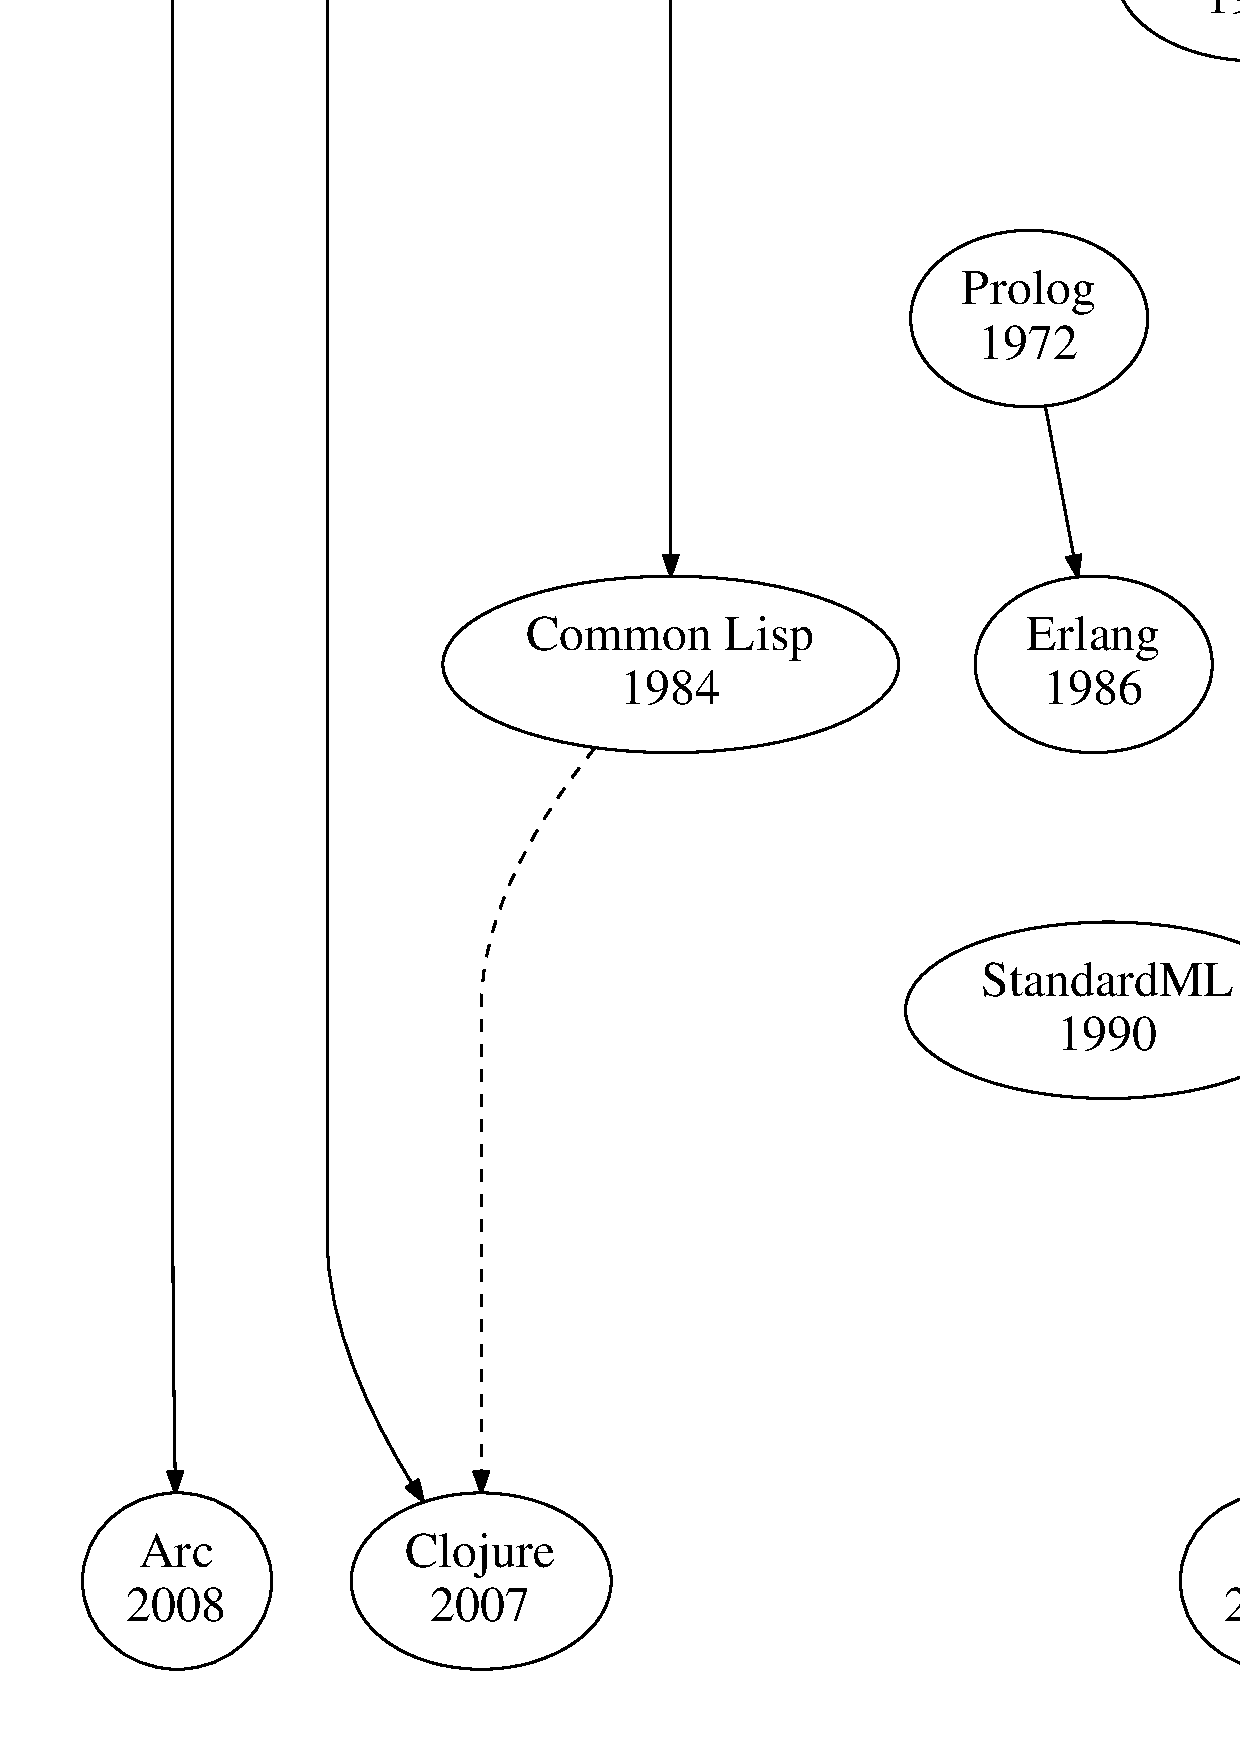
\includegraphics[width=\textwidth]{languages.pdf}
  \else
    \includegraphics[width=\textwidth]{languages.ps}
  \fi
\caption{Родословное древо функциональных языков}
\label{lineage}
\end{figure}

Как уже упоминалось в разделе \ref{benefits}, функциональные языки существуют довольно давно. Первый из них, Лисп, создан в 1958 году, всего на год позже первого императивного языка~--- Фортрана. Ещё один известный функциональный язык, РЕФАЛ, создан В.Ф.Турчиным в 1966 году. Но если РЕФАЛ стал широко известен довольно поздно (возможно, по причинам, далёким от программирования: он был создан в СССР в эпоху Холодной войны, а ФП развивалось в то время в основном по другую сторону Железного занавеса), то распространение Лиспа продолжалось всё время его существования. Уже в двухтысячных годах появились два новых популярных диалекта этого языка: Arc и Clojure.

Наиболее известные диалекты Лиспа~--- Common Lisp и Scheme. Первый чаще других вариантов Лиспа применяется на практике, а вторая используется в основном для обучения программированию. К сожалению, непоследовательная политика стандартизации сильно замедлила распространение Scheme как языка практического программирования.

Изучение Лиспа (скорее всего, Scheme) практически неизбежно для человека, интересущегося функциональным программированием, так как многие важные работы на эту тему используют именно Scheme в качестве языка примеров. Среди возможностей Scheme, отсутствующих в Эрланге, особенно интересны  продолжения (continuations)~--- способ сохранять как значение состояние программы в определённый момент.

Второй после Лиспа по влиятельности и многочисленности <<потомства>> функциональный язык это ML. В нём впервые была реализована очень мощная техника~--- {\em вывод типов}, то есть автоматическое определение компилятором типа выражения по контексту, в котором оно используется. Вывод типов избавляет программиста от целого класса неприятных ошибок. В этой книжке я использовал язык без вывода типов\footnote{На самом деле, похожие инструменты для Эрланга реализованы, но они гораздо слабее своих аналогов из языков-потомков ML.} только потому, что это сильно усложнило и удлинило бы курс.

Наиболее известные потомки ML это OCaml, F\# (построенный на базе OCaml язык для платформы .Net) и Haskell.

Именно Haskell считается <<передним краем>> исследований в области функционального программирования. В практическом программировании он применяется не так часто, возможно, потому, что его авторы очень жёстко отказываются вносить в язык полезные для индустрии, но <<некрасивые>> с точки зрения теории возможности~--- полушутливый девиз Haskell это <<Avoid success at all costs>> (<<Избегать успеха любой ценой>>). Пожалуй, Haskell~--- это второй после Scheme язык, изучения которого интересующемуся ФП человеку вряд ли удастся избежать. Изучить этот язык стоит хотя бы для того, чтобы познакомиться с такими интереснейшими концепциями, как ленивые вычисления или монады.

К сожалению, малопопулярен другой замечательный диалект ML~--- StandardML, очень красивый, гораздо более компактный, чем Haskell (и, на мой взгляд, более логичный синтаксически, чем OCaml и F\#) язык.

Ну и, наконец, не надо забывать, что Эрланг мы тоже изучили не до конца. Если вам понравился Эрланг, стоит всерьёз заняться изучением его возможностей. На самом деле, в этом курсе вообще не используется одно из главных преимуществ Эрланга~--- библиотека OTP, Open Telecom Platform, предоставляющая готовые решения для задач параллельного и распределённого программирования. <<За кадром>> остались также поведения (behaviours), обработка исключительных ситуаций, макросы и многое другое.

\section{Что ещё можно почитать про ФП}

Функциональному программированию посвящено довольно много книг, ресурсов в Интернете и журналов. Хорошей стартовой точкой для дальнейшего знакомства с миром ФП может стать журнал <<Практика функционального программирования>>, свободно доступный на сайте \url{http://fprog.ru/}. Кстати, в первом номере журнала опубликован обзор литературы по функциональному программированию, сделанный Алексеем Оттом~\cite{PFP_Ott}.

Ещё одна хорошая обзорная статья~--- <<Функциональное программирование для всех>> В.Ахмечета~\cite{Akhmechet}, опубликованная в журнале RSDN Magazine.

Среди книг прежде всего надо упомянуть <<Структуру и интерпретацию компьютерных программ>> Х.Абельсона и Дж.Сассмана~\cite{SICP}, которая по праву считается классической. Это учебник по программированию вообще, не только функциональному, но значительная часть материала изложена именно с помощью функциональных решений.

Большинство работ по алгоритмам и структурам данных расчитано на императивные языки. Эту ситуацию пытается исправить Крис Окасаки, автор книги <<Чисто функциональные структуры данных>>~\cite{Okasaki}. Ещё одна серьёзная работа по теоретическим аспектам программирования, ориентированная на ФП~--- <<Типы в языках программирования>> Б.Пирса~\cite{Pierce}.

Очень хороший пример практического программирования на функциональных языках приводится в статье Д.Астапова <<Давно не брал я в руки шашек>>~\cite{PFP_Astapov}. Интересующимся продвинутыми программистскими техниками будет, вероятно, интересно прочитать статьи А.Вознюка о продолжениях~\cite{PFP_Voznyuk} и И.Ключникова о суперкомпиляции~\cite{PFP_Klyuchnikov}. Впрочем, как уже говорилось, журнал <<Практика функционального программирования>>, в котором опубликованы все эти статьи, вообще рекомендуется к ознакомлению при наличии интереса к теме.

Замечательные учебники по языку Scheme и функциональному программированию~--- книги <<Little Schemer>>~\cite{little_schemer} и <<Seasoned Schemer>>~\cite{seasoned_schemer}, к сожалению, в отличие от SICP не переведены на русский язык.

Хороший вводный материал по языку Haskell~--- цикл статей Алексея Бешенова~\cite{Beshenov} и книга <<Изучай Haskell во имя добра!>>~\cite{Lipovacha}, а если говорить об источниках на английском языке~--- <<Real World Haskell>>~\cite{real_world_haskell}. По Стандартному ML на русском издана книга Р.Харпера <<Введение в Стандартный ML>>~\cite{Harper}.

Про возможности OTP, концепцию <<поведений>> (behaviours) можно прочитать в книге \cite{cesarini}. Из важных книг по Эрлангу, пока не переведённых на русский язык, надо упомянуть учебник Дж.Армстронга (создателя языка)~\cite{armstrong} и книгу <<Erlang and OTP in action>>~\cite{OTP_in_action}. Хороший вводный курс, правда, во многом дублирующий уже изложенное здесь~--- <<Learn You Some Erlang for Great Good>>~\cite{LYSE}.

\chapter*{Решения задач}
\addcontentsline{toc}{chapter}{Решения задач}
\markboth{Решения задач}{Азбука ФП}

\section*{Азбука ФП}
\addcontentsline{toc}{section}{Азбука ФП}

\solution{nand}

\lstinputlisting{abc/nand/logic.erl}

Вообще говоря, функцию \lstinline{nand} можно было бы определить гораздо проще:

\begin{lstlisting}
nand(true, true) -> false;
nand(_, _) -> true.
\end{lstlisting}

Но этот вариант функции \lstinline{nand} не будет выдавать ошибку, если передать ему в качестве аргументов что-то помимо атомов\index{Атом} \lstinline{true} и \lstinline{false}, что может затруднить поиск источника проблемы в неправильно написанной программе. Поэтому лучше перечислить все корректные варианты аргументов явно.

Помните, в Эрланге принят подход <<Let it fail>>~--- <<Пусть падает>>.

\solution{myor}

\lstinputlisting{abc/logic.erl}

\solution{author}

\lstinputlisting{abc/author.erl}

\solution{sign}

\lstinputlisting{abc/sign.erl}

\solution{divisor}

\lstinputlisting{abc/divisor.erl}

\solution{summ}

\lstinputlisting{abc/summ.erl}

\solution{divisors}

\lstinputlisting{abc/divisors.erl}

\solution{remainder}

\lstinputlisting{abc/remainder.erl}

\solution{number_sequence}

\lstinputlisting{abc/number_input.erl}

Эту задачу можно решить и иначе~--- например, вот так:

\lstinputlisting{abc/number_input/number_input.erl}

Идея решения та же самая, а как её оформить~--- вопрос вкуса. В таком варианте приодится дублировать оператор ввода, зато вместо \lstinline{case} используется сопоставление с образцом\index{Сопоставление с образцом}, что, по идее, должно делать код более понятным.

\solution{rember}

\lstinputlisting{abc/rember.erl}

\solution{listrev}

\lstinputlisting{abc/listrev.erl}

\solution{slice}

\lstinputlisting[language=erlang]{sugar/slice.erl}

\solution{flatten}

Алгоритм решения этой задачи можно коротко описать так: мы создаём временный список для хранения текущего разбираемого элемента (второй аргумент функции \lstinline{flatten/2}). Поначалу он пуст (это тот второй аргумент, который передаёт функции \lstinline{flatten/2} функция \lstinline{flatten/1}).

Если исходный список тоже пуст, то работа закончена (первый вариант функции).

Если исходный список не пуст, то мы берём его голову и помещаем во временный список для разбора (второе тело функции).

Если текущий разбираемый элемент это тоже список, то мы берём его голову, а хвост возвращаем в исходный список, где он будет дожидаться своей очереди (третье тело функции).

Наконец, если ни одно из предыдущих сопоставлений с образцом\index{Сопоставление с образцом} не увенчалось успехом, надо полагать, что хранилище разбираемых элементов не пусто (иначе бы сработали бы образцы 1 или 2) и то, что в нём лежит~--- не список (иначе сработал бы образец 3). Следовательно, это одиночное значение и мы можем смело помещать его в голову итогового списка.

\lstinputlisting{abc/flatten.erl}

\solution{palindrome}

\lstinputlisting[language=erlang]{best_practices/palindrome.erl}

\solution{perfect}
Функция \lstinline{divisors}, составляющая список делителей числа $N$, лежащих в интервале от 1 до $M$ включительно~--- это попросту индуктивное определение такого списка: если он заканчивается единицей, то только единица в него и войдёт, а если он должен состоять из чисел в интервале от единицы до некоего числа $M$, большего, чем единица, то в него войдут делители числа $N$ в интервале от 1 до $M-1$, а также само $M$, если оно тоже является делителем $N$.

Случай с единицей мы обрабатываем в \lstinline{divisors/1}, чтобы избежать лишнего вызова функции.

Функция \lstinline{lists:sum} из модуля \lstinline{lists}, подсчитывающая сумму списка чисел, ощутимо упрощает решение этой задачи.

Обратите внимание, что функция \lstinline{divisors} небезопасна и будет зацикливаться при значениях $M$ меньше 1. Здесь было разумным пожертвовать безопасностью в ущерб ясности; в реальных программах часто полезно делать наоборот.
\lstinputlisting[language=erlang]{abc/perfect.erl}
\pagebreak

\solution{brackets}
В этой задаче можно представлять строку для разбора либо как обычный эрланговский список, либо как битовую строку. Решение с битовыми строками чуть более громоздко, но в реальной жизни битовые строки гораздо полезнее <<строк>>, хранящихся как списки ASCII-кодов.

Алгоритм же в обоих решениях~--- один и тот же: сделаем стек, в который будем класть все открывающие скобки. Встречая закрывающую скобку, будем выпихивать со стека верхнее значение. Если тип закрывающей скобки из текущей позиции строки и открывающей скобки с вершины стека не совпали (или стек пуст), порядок скобок неправильный. Если после того, как вся строка разобрана, в стеке что-то осталось, порядок скобок тоже неправильный. Если же нам удалось подойти к концу строки с пустым стеком (или строка просто пустая), значит, порядок скобок~--- правильный.

\begin{figure}[!t,bracketspic]
\centerline{
\begin{pspicture}%[showgrid=true]
(10, 11)
\rput(2, 10.5){Входной список}
\rput(6.8, 10.5) {Стек}
\rput(0, 9){
  % Входной список
  \psgrid[gridlabels=0.0pt,subgriddiv=1](0,0)(0,0)(5,1)
  \rput(0.5, 0.5){[}
  \rput(1.5, 0.5){(}
  \rput(2.5, 0.5){<}
  \rput(3.5, 0.5){)}
  \rput(4.5, 0.5){]}
  % Операция
  \psbezier{->}(0.5,0)(0.5,-1)(6.5,0)(6.5,-1)
}
\rput(0, 7) {
  % Входной список
  \psgrid[gridlabels=0.0pt,subgriddiv=1](0,0)(0,0)(4,1)
  \rput(0.5, 0.5){(}
  \rput(1.5, 0.5){<}
  \rput(2.5, 0.5){)}
  \rput(3.5, 0.5){]}
  % Операция
  \psbezier{->}(0.5,0)(0.5,-1)(6.5,0)(6.5,-1)
  % Стек
  \psgrid[gridlabels=0.0pt,subgriddiv=1](0,0)(6,0)(7,1)
  \rput(6.5, 0.5){(}
}
\rput(0, 5) {
  % Входной список
  \psgrid[gridlabels=0.0pt,subgriddiv=1](0,0)(0,0)(3,1)
  \rput(0.5, 0.5){<}
  \rput(1.5, 0.5){)}
  \rput(2.5, 0.5){]}
  % Операция
  \psbezier{->}(0.5,0)(0.5,-1)(6.5,0)(6.5,-1)
  % Стек
  \psgrid[gridlabels=0.0pt,subgriddiv=1](0,0)(6,0)(8,1)
  \rput(6.5, 0.5){(}
  \rput(7.5, 0.5){[}
}
\rput(0, 3) {
  % Входной список
  \psgrid[gridlabels=0.0pt,subgriddiv=1](0,0)(0,0)(2,1)
  \rput(0.5, 0.5){)}
  \rput(1.5, 0.5){]}
  % Операция
  \psbezier{->}(0.5,0.0)(0.5,-1)(0.5,-1)(3.5,-1)
  \psbezier{->}(6.5,0.0)(6.5,-1)(6.5,-1)(4.5,-1)
  \rput(4, -1){\pscirclebox{?}}
  \psline{->}(4,-1.5)(4,-2)
  % Стек
  \psgrid[gridlabels=0.0pt,subgriddiv=1](0,0)(6,0)(9,1)
  \rput(6.5, 0.5){<}
  \rput(7.5, 0.5){(}
  \rput(8.5, 0.5){[}
  % Возвращаемое значение
  \rput(4, -2.5){false}
  \psbezier{->}(4.75,-2.5)(5.5,-3)(5.5,-2)(6.25,-2.5)
  \rput(7, -2.5){false}
}
\end{pspicture}
}
\caption{Функция \lstinline{is_valid_string/2} проверяет скобочную структуру <<[(<)]>> на правильность. Слева~--- входной список (первый аргумент функции), справа~--- стек (второй аргумент функции).}
\label{bracketspic}
\end{figure}

\lstinputlisting[language=erlang]{abc/brackets_str.erl}
\pagebreak
\lstinputlisting[language=erlang]{abc/brackets.erl}
\pagebreak

\solution{queue}

Идея решения вот в чём: реализуем очередь как два списка, входной и выходной. При помещении значения в очередь будем добавлять его в голову входного списка. При извлечении значения из очереди проверим, пуст ли выходной список. Если да, проверим, пуст ли входной. Если пуст и он, очередь пуста (второй вариант тела функции). А если входной список не пуст, развернём его, отдадим голову получившегося списка как выходное значение, а хвост поместим в выходной список (входной список, соответственно, становится пустым). Эти действия описаны в первом варианте тела функции. Ну а если выходной список не пуст, просто отдаём его голову, т.к. значения в нём уже стоят в правильном порядке (третий вариант тела функции).

Работа с организованной таким образом очередью будет выглядеть примерно так.

\begin{figure}[!t,queuepic]
\centerline{
\begin{pspicture}%[showgrid=true]
(9, 21)
\rput(3.0, 20.5){Входной}
\rput(3.0, 19.5){список}
\rput(6.0, 20.5){Выходной}
\rput(6.0, 19.5){список}
\rput(0, 18) {
  \psframe[linestyle=dotted](1.8,-0.2)(7.2, 1.2)
  % Операция
  \rput(0.5, 0.5){1}
  \psline{->}(0.8, 0.5)(1.6, 0.5)
}
\rput(0, 16) {
  \psframe[linestyle=dotted](1.8,-0.2)(7.2, 1.2)
  % Входной список
  \psgrid[gridlabels=0.0pt,subgriddiv=1](0,0)(2,0)(3,1)
  \rput(2.5, 0.5){1}
  % Операция
  \rput(0.5, 0.5){2}
  \psline{->}(0.8, 0.5)(1.6, 0.5)
}
\rput(0, 14) {
  \psframe[linestyle=dotted](1.8,-0.2)(7.2, 1.2)
  % Входной список
  \psgrid[gridlabels=0.0pt,subgriddiv=1](0,0)(2,0)(4,1)
  \rput(2.5, 0.5){2}
  \rput(3.5, 0.5){1}
  % Операция
  \rput(0.5, 0.5){3}
  \psline{->}(0.8, 0.5)(1.6, 0.5)
}
\rput(0, 12) {
  \psframe[linestyle=dotted](1.8,-0.2)(7.2, 1.2)
  % Операция
  \rput(8.5, 0.5){1}
  \psline{->}(7.4, 0.5)(8.2, 0.5)
  % Выходной список
  \psgrid[gridlabels=0.0pt,subgriddiv=1](0,0)(5,0)(7,1)
  \rput(5.5, 0.5){3}
  \rput(6.5, 0.5){2}
}
\rput(0, 10) {
  \psframe[linestyle=dotted](1.8,-0.2)(7.2, 1.2)
  % Операция
  \rput(0.5, 0.5){4}
  \psline{->}(0.8, 0.5)(1.6, 0.5)
  % Выходной список
  \psgrid[gridlabels=0.0pt,subgriddiv=1](0,0)(5,0)(7,1)
  \rput(5.5, 0.5){3}
  \rput(6.5, 0.5){2}
}
\rput(0, 8) {
  \psframe[linestyle=dotted](1.8,-0.2)(7.2, 1.2)
  % Входной список
  \psgrid[gridlabels=0.0pt,subgriddiv=1](0,0)(2,0)(3,1)
  \rput(2.5, 0.5){4}
  % Операция
  \rput(0.5, 0.5){5}
  \psline{->}(0.8, 0.5)(1.6, 0.5)
  % Выходной список
  \psgrid[gridlabels=0.0pt,subgriddiv=1](0,0)(5,0)(7,1)
  \rput(5.5, 0.5){3}
  \rput(6.5, 0.5){2}
}
\rput(0, 6) {
  \psframe[linestyle=dotted](1.8,-0.2)(7.2, 1.2)
  % Входной список
  \psgrid[gridlabels=0.0pt,subgriddiv=1](0,0)(2,0)(4,1)
  \rput(2.5, 0.5){5}
  \rput(3.5, 0.5){4}
  % Операция
  \rput(8.5, 0.5){2}
  \psline{->}(7.4, 0.5)(8.2, 0.5)
  % Выходной список
  \psgrid[gridlabels=0.0pt,subgriddiv=1](0,0)(6,0)(7,1)
  \rput(6.5, 0.5){3}
}
\rput(0, 4) {
  \psframe[linestyle=dotted](1.8,-0.2)(7.2, 1.2)
  % Входной список
  \psgrid[gridlabels=0.0pt,subgriddiv=1](0,0)(2,0)(4,1)
  \rput(2.5, 0.5){5}
  \rput(3.5, 0.5){4}
  % Операция
  \rput(8.5, 0.5){3}
  \psline{->}(7.4, 0.5)(8.2, 0.5)
}
\rput(0, 2) {
  \psframe[linestyle=dotted](1.8,-0.2)(7.2, 1.2)
  % Операция
  \rput(8.5, 0.5){4}
  \psline{->}(7.4, 0.5)(8.2, 0.5)
  % Выходной список
  \psgrid[gridlabels=0.0pt,subgriddiv=1](0,0)(6,0)(7,1)
  \rput(6.5, 0.5){5}
}
\rput(0, 0) {
  \psframe[linestyle=dotted](1.8,-0.2)(7.2, 1.2)
  % Операция
  \rput(8.5, 0.5){5}
  \psline{->}(7.4, 0.5)(8.2, 0.5)
}
\end{pspicture}
}
\caption{Организация очереди из двух списков.}
\label{queuepic}
\end{figure}

Компилируем модуль, загружаем определение записи:
\erlshell{c(listqueue).}{\{ok,listqueue\}}
\erlshell{rr("queue.hrl").}{{[}queue{]}}

Создаём новую очередь:
\erlshell{Q1 = \#queue\{\}.}{\#queue\{in = [],out = []\}}

Помещаем в очередь значение 1:
\erlshell{Q2 = listqueue:enqueue(Q1, 1).}{\#queue\{in = [1],out = []\}}

Помещаем в очередь значение 2:
\erlshell{Q3 = listqueue:enqueue(Q2, 2).}{\#queue\{in = [2,1],out = []\}}

Помещаем в очередь значение 3:
\erlshell{Q4 = listqueue:enqueue(Q3, 3).}{\#queue\{in = [3,2,1],out = []\}}

Извлекаем из очереди первое значение (1)~--- в этот момент входной список будет развёрнут и перемещён в выходной:
\erlshell{\{ok, Out1, Q5\} = listqueue:dequeue(Q4).}{\{ok,1,\#queue\{in = [],out = [2,3]\}\}}
\erlshell{Out1.}{1}

Добавляем в очередь значение 4 (с этого момента формируется новый входной список):
\erlshell{Q6 = listqueue:enqueue(Q5, 4).}{\#queue\{in = [4],out = [2,3]\}}

Добавляем в очередь значение 5:
\erlshell{Q7 = listqueue:enqueue(Q6, 5).}{\#queue\{in = [5,4],out = [2,3]\}}

Извлекаем из очереди второе значение (2):
\erlshell{\{ok, Out2, Q8\} = listqueue:dequeue(Q7).}{\{ok,2,\#queue\{in = [5,4],out = [3]\}\}}

Извлекаем из очереди третье значение (3):
\erlshell{\{ok, Out3, Q9\} = listqueue:dequeue(Q8).}{\{ok,3,\#queue\{in = [5,4],out = []\}\}}

Извлекаем из очереди четвёртое значение (4)~--- выходной список пуст, снова разворачиваем входной список и перемещаем его на место опустевшего выходного:
\erlshell{\{ok, Out4, Q10\} = listqueue:dequeue(Q9).}{\{ok,4,\#queue\{in = [],out = [5]\}\}}

Извлекаем из очереди пятое значение (5):
\erlshell{\{ok, Out5, Q11\} = listqueue:dequeue(Q10).}{\{ok,5,\#queue\{in = [],out = []\}\}}

Очередь пуста, при попытке извлечения дальнейших значений будет возвращена информация об ошибке:
\erlshell{listqueue:dequeue(Q11).}{\{error,"Queue is empty"\}}

Несмотря на наличие в этом алгоритме <<тяжёлой>> операции разворачивания списка, требующей $N$ шагов для списка из $N$ элементов, условиям задачи он отвечает, т.к. каждый проходящий через очередь элемент участвует в этой операции только один раз.

\lstinputlisting[language=erlang]{abc/listqueue.erl}

\solution{node_cut}

Обратите внимание на то, как функции \lstinline{trim/2} и \lstinline{trim/3} рекурсивно вызывают друг друга. Это полезный приём, который позволяет упростить отладку и тестирование, а также улучшить читаемость кода за счёт избавления от громоздких операторов ветвления.

\lstinputlisting[language=erlang]{abc/trimtree.erl}

\solution{node_count}

\lstinputlisting[language=erlang]{abc/treemeter.erl}

\section*{Полезные приёмы}
\addcontentsline{toc}{section}{Полезные приёмы}
\markright{Полезные приёмы}

\solution{already}

Хвостовая рекурсия уже используется в решениях задач \ref{summ}, \ref{divisors}, \ref{remainder}, \ref{listrev}, \ref{brackets}.

\solution{tail}

Функцию \lstinline{rember/2} из задачи \ref{rember} можно переписать следующим образом:

\lstinputlisting[language=erlang]{abc/tailrember.erl}

Проблема в том, что такой способ обработки списка разворачивает его, и нам приходится вызывать \lstinline{lists:reverse}, чтобы вернуть исходный порядок следования элементов. Поэтому применение здесь хвостовой рекурсии не очень оправдано. В решениях других задач применение хвостовой рекурсии принесёт ещё больше сложностей.

Не надо применять хвостовую рекурсию по любому поводу. Во-первых, она не всегда эффективнее обычной, во-вторых, помните: сначала стабильная работа программы, потом оптимизация.

\solution{perfect_list}

\lstinputlisting[language=erlang]{best_practices/perfect.erl}
\pagebreak

\solution{maptree}

\lstinputlisting[language=erlang]{best_practices/maptree.erl}

\solution{length}
\begin{lstlisting}
lists:foldl(fun(_, Length) -> Length + 1 end, 0, L).
\end{lstlisting}

\solution{foldrev}

\lstinputlisting[language=erlang]{best_practices/foldrev.erl}

\solution{mean}

\lstinputlisting[language=erlang]{best_practices/mean.erl}

\solution{foldl1}

\lstinputlisting[language=erlang]{best_practices/mylists.erl}

\solution{foldseq}

\lstinputlisting[language=erlang]{best_practices/myseq.erl}

\solution{ismemberof}

\lstinputlisting[language=erlang]{best_practices/ismemberof.erl}

\section*{Приятные мелочи}
\addcontentsline{toc}{section}{Приятные мелочи}
\markright{Приятные мелочи}

\solution{short_perfect}

\lstinputlisting[language=erlang]{sugar/perfect.erl}

\solution{common}

\lstinputlisting[language=erlang]{sugar/common_members.erl}

\solution{multiplication}

\lstinputlisting[language=erlang]{best_practices/multiplication.erl}

\solution{common_without_member}

\lstinputlisting[language=erlang]{sugar/common2.erl}

\solution{queens}

\lstinputlisting[language=erlang]{sugar/queens.erl}

%% Решение из статьи про задачу в Википедии %% (http://ru.wikipedia.org/wiki/%D0%97%D0%B0%D0%B4%D0%B0%D1%87%D0%B0_%D0%BE_%D0%B2%D0%BE%D1%81%D1%8C%D0%BC%D0%B8_%D1%84%D0%B5%D1%80%D0%B7%D1%8F%D1%85#.D0.A0.D0.B5.D0.B0.D0.BB.D0.B8.D0.B7.D0.B0.D1.86.D0.B8.D1.8F_.D0.BD.D0.B0_Erlang):

%% pmut([])->
%%         [[]];
%% pmut(A) ->
%%         [[H|T] || H <- A, T <- pmut(A--[H])].
 
%% start() ->
%%         N = 8, % size of board / num of queens (N>=4)
%%         ListP = pmut(lists:seq(1,N)),
%%         [Q || Q <- ListP, length(lists:usort([lists:nth(X,Q)+X || X <- %% Q])) == N, 
%%         length(lists:usort([lists:nth(X,Q)-X || X <- Q])) == N]

\solution{foldrrev}

\lstinputlisting[language=erlang]{sugar/foldrrev.erl}

\solution{linearize}

\lstinputlisting[language=erlang]{sugar/trees-linearize/trees.erl}

\solution{hanoi}

Сформулируем принципы перекладывания стопки из $N$ дисков.

Базовый случай в этой задаче~--- $N=0$, т.е. ситуация, когда нам ничего перекладывать не нужно. Большее количество дисков перекладывается по следующему алгоритму (стержень, с которого перемещаем диски, будем называть исходным, стержень, на который перемещаем диски~--- целевым, а третий~--- вспомогательным):

\begin{enumerate}
\item Взять $N-1$ дисков и переместить их с исходного стержня на вспомогательный.
\item Переместить оставшийся на исходном стержне диск на целевой стержень.
\item Переместить $N-1$ дисков со вспомогательного стержня на целевой.
\end{enumerate}

Первый и третий шаги предполагают перекладывание стопки дисков, то есть рекурсивный вызов процедуры перекладывания. Но так как в каждом следующем вызове $N$ гарантированно уменьшается, мы можем быть уверены, что рано или поздно рекурсия закончится.

\lstinputlisting[language=erlang]{sugar/hanoi.erl}

\solution{dropwhile}

Сложность с реализацией \lstinline{dropwhile} в том, что реакция на элемент, для которого переданная функция возвращает \lstinline{true}, должна отличаться в зависимости от того, встретился ли нам уже элемент, для которого эта функция вернула \lstinline{false}. Так как мы имеем дело со свёрткой\index{Свёртка списка}, мы не можем ввести какой-то дополнительный параметр, указывающий, так ли это~--- ведь тогда свёртка вернёт его вместе с итоговым списком, а это не то, что нам нужно.

Но на самом деле при левой свёртке\index{Свёртка списка!левая} таким параметром является сам итоговый список: если он пуст, значит, не отвечающий критерию элемент нам ещё не встречался и мы должны проверить текущий элемент с помощью функции-аргумента. Если список не пуст, мы должны безо всяких проверок поместить в него текущий элемент.

\lstinputlisting[language=erlang]{best_practices/dropwhile.erl}

Реализовать \lstinline{dropwhile} с помощью правой свёртки\index{Свёртка списка!правая}, строго говоря, невозможно~--- правая свёртка начинается с конца списка, что не позволяет нам найти первое с начала списка вхождение элемента с её помощью. Но динамическая типизация Эрланга позволяет нам реализовать обходное решение, жульническое по сути (реальная работа делается вне свёртки), но позволяющее <<обмануть>> функцию \lstinline{foldr}, подсунув ей функцию, которая формально удовлетворяет условиям задачи:

\lstinputlisting[language=erlang]{best_practices/rdropwhile.erl}

Идея этого решения в следующем: мы заранее находим первый элемент в списке, для которого функция \lstinline{F} вернёт \lstinline{false} и запоминаем его позицию (далее будем называть её <<линией отреза>>. После этого мы определяем функцию \lstinline{Trim}, у которой есть два варианта списка аргументов: либо текущий элемент списка и кортеж вида {\em \{Накопленный хвост списка, Позиция текущего элемента, Линия отреза\}}, либо текущий элемент и список.

\lstinline{Trim} будет добавлять к накопленному хвосту списка элемент за элементом, пока позиция текущего элемента не совпадёт с линией отреза. В этот момент она оставит в аргументе-накопителе только список. Следующие вызовы, обнаружив во втором аргументе список вместо кортежа, просто передадут аргумент-накопитель дальше.

Обратите внимание, что ситуация, когда элемент, для которого \lstinline{F} возвращает \lstinline{false}, так и не был найден, требует особой обработки.

Надо ещё раз подчеркнуть, что это решение является хаком в самом плохом смысле этого слова и непереносимо на многие функциональные языки с более строгим контролем типов, вроде Стандартного ML и Haskell (решения, построенные на аналогичной идее, пожалуй, возможны и там, но ценой ещё более уродливых ухищрений).

\solution{permutations}

Идея решения этой задачи вот в чём. В список перестановок списка длины $1$ входит единственный элемент~--- он сам. А перестановки списка большей длины можно получить так: по очереди удалять из списка каждый элемент, получать все перестановки оставшихся и в начало каждой из них подставлять удалённый элемент.

% Я видел где-то лучшее решение с --

\lstinputlisting[language=erlang]{sugar/permutations.erl}

\section*{От функционального программирования к параллельному}
\addcontentsline{toc}{section}{От функционального программирования к параллельному}
\markright{От ФП к ПП}

\solution{approximation}

\lstinputlisting[language=erlang]{parallel/montecarlo.erl}

\solution{fibmem}

\lstinputlisting[language=erlang]{parallel/fibmem.erl}

% Приложение: отладчик, запускающийся по debugger:start()? Трассировщик, если он может быть чем-то полезен? EUnit?

% Приложение: установка Эрланга на разных платформах?

\addcontentsline{toc}{chapter}{Литература}
\begin{thebibliography}{99}
\bibitem[Абельсон 2010]{SICP}
Абельсон Х., Сассман Дж. Дж. Структура и интерпретация компьютерных программ. М.: <<Добросвет>>, <<КДУ>>, 2010.
\bibitem[Астапов 2009]{PFP_Astapov}
Астапов Д. Давно не брал я в руки шашек // Практика функционального программирования, №1, 2009.
\bibitem[Ахмечет 2006]{Akhmechet}
Ахмечет В. Функциональное программирование для всех. // RSDN Magazine, №2, 2006.
\bibitem[Бешенов 2010]{Beshenov}
Бешенов А. Функциональное программирование на Haskell.\\
\href{http://www.ibm.com/developerworks/ru/library/l-haskell/}{Часть 1. Введение.}\\
\href{http://www.ibm.com/developerworks/ru/library/l-haskell2/}{Часть 2.Основные типы и классы.}\\
\href{http://www.ibm.com/developerworks/ru/library/l-haskell3/}{Часть 3. Определение функций.}\\
\href{http://www.ibm.com/developerworks/ru/library/l-haskell4/}{Часть 4. Свертки списков.}
\bibitem[Вознюк 2011]{PFP_Voznyuk}
Вознюк А. Продолжения в практике. // Практика функционального программирования, №7, 2011.
\bibitem[Златопольский 2007]{zlatopolsky}
Златопольский Д.М. Программирование: типовые задачи, алгоритмы, методы. М., 2007.
\bibitem[Ключников 2011]{PFP_Klyuchnikov}
Ключников И. Суперкомпиляция: идеи и методы. // Практика функционального программирования, №7, 2011.
\bibitem[Липовача 2012]{Lipovacha}
Липовача М. Изучай Haskell во имя добра! М.: <<ДМК Пресс>>, 2012.
\bibitem[Отт 2009]{PFP_Ott}
Отт А. Обзор литературы о функциональном программировании. // Практика функционального программирования, №1, 2009.
\bibitem[Пирс 2012]{Pierce}
Пирс Б., Типы в языках программирования. М.: <<Лямбда пресс>>, <<Добросвет>>, 2012.
\bibitem[Харпер 1996]{Harper}
Харпер Р. Введение в Стандартный ML. М., 1996.
\bibitem[Чезарини 2012]{cesarini}
Чезарини Ф., Томпсон С. Программирование в Эрланг. М.: <<ДМК Пресс>>,
2012.
\bibitem[Шень 2004]{shen}
Шень А. Программирование: теоремы и задачи. М.: МЦНМО, 2004.
\bibitem[99 problems]{99problems}
99 Problems на выбранном языке (точно есть для \href{http://www.haskell.org/haskellwiki/99_questions}{Haskell}, \href{http://aperiodic.net/phil/scala/s-99/}{Scala}, \href{https://sites.google.com/site/prologsite/prolog-problems}{Prolog}, \href{http://www.christiankissig.de/cms/index.php/en/programming/28-ocaml/28-99-problems-in-ocaml}{OCaml}, \href{http://www.informatimago.com/develop/lisp/l99/index.html}{Common Lisp}).
\bibitem[Armstrong 2007]{armstrong}
Armstrong J. Programming Erlang: Software for a Concurrent World. Pragmatic Bookshelf, 2007.
\bibitem[Friedman 1996]{little_schemer}
Friedman D.P., Fellsen M. The Little Schemer. MIT Press, 1996.
\bibitem[Friedman 1996,2]{seasoned_schemer}
Friedman D.P., Fellsen M. The Seasoned Schemer. MIT Press, 1996.
\bibitem[LYSE]{LYSE}
Learn You Some Erlang for Great Good, \url{http://learnyousomeerlang.com/}.
\bibitem[Logan 2011]{OTP_in_action}
Logan M., Merritt E., Carlsson R. Erlang and OTP in action. Manning Publications, 2011.
\bibitem[Miller]{miller}
Evan Miller. The Joy of Erlang; Or, How To Ride A Toruk, \url{http://www.evanmiller.org/joy-of-erlang.html}.
\bibitem[Okasaki 1999]{Okasaki}
Okasaki C. Purely Functional Data Structures. Cambridge University Press, 1999.
\bibitem[O'Sullivan 2008]{real_world_haskell}
O'Sullivan B., Goerzen J., D.B. Stewart. Real World Haskell. Code You Can Believe In. O'Reilly, 2008.
\end{thebibliography}

\appendix

\pagebreak
\addcontentsline{toc}{chapter}{Приложения}

\chapter{Краткий справочник по используемым функциям}

\section*{Ввод-вывод}
\addcontentsline{toc}{section}{Ввод-вывод}
\markright{Ввод-вывод}

Здесь приводятся только те функции, которые требуются для той или иной задачи. С полной документацией на упомянутые модули можно ознакомиться на сайте языка: \url{http://erlang.org/doc/}.

\begin{funcdescr}
\funcdoc{io:format/1}{Принимает строку с командами формата и выводит её на экран.}
\funcdoc{io:format/2}{Принимает строку с командами формата и список подставляемых значений; выводит на экран строку, в которую подставлены значения в соответствии с командами формата.}
\funcdoc{io:fread/2}{Принимает подсказку и строку формата; читает со стандартного ввода выражения и пытается привести их к типам, заданным строкой формата; в случае успеха возвращает кортеж из атома \lstinline{ok} и списка прочитанных значений, в случае  ошибки~--- кортеж из атома \lstinline{error} и описания ошибки.}
\funcdoc{io:read/1}{Принимает подсказку для ввода; читает со стандартного ввода выражение Эрланга и возвращает кортеж из атома \lstinline{ok} и прочитанного выражения в случае успеха либо кортеж из атома \lstinline{error} и описания ошибки в случае ошибки.}
\end{funcdescr}

\section*{Математика}
\addcontentsline{toc}{section}{Математика}
\markright{Математика}

\begin{funcdescr}
\funcdoc{abs/1}{Возвращает модуль числа.}
\funcdoc{math:sqrt/1}{Возвращает квадратный корень своего аргумента.}
\funcdoc{random:uniform/0}{Возвращает случайное вещественное число в интервале от 0.0 до 1.0.}
\funcdoc{random:uniform/1}{Возвращает случайное целое число в интервале от 1 до своего аргумента.}
\end{funcdescr}

\section*{Обработка списков}
\addcontentsline{toc}{section}{Обработка списков}
\markright{Обработка списков}

\begin{funcdescr}
\funcdoc{length/1}{Принимает список; возвращает длину этого списка.}
\funcdoc{lists:dropwhile/2}{Принимает функцию-тест и список; возвращает список, из которого выброшены все элементы до первого, для которого функция-тест вернула \lstinline{false}.}
\funcdoc{lists:filter/2}{Принимает функцию-тест и список; возвращает список, в котором оставлены только те элементы, для которых функция-тест вернула \lstinline{true}.}
\funcdoc{lists:foldl/3}{Левая свёртка: принимает функцию, начальное значение накопителя и список. Функция-аргумент должна принимать два параметра: текущее значение накопителя и текущий элемент списка, а возвращать новое значение накопителя. Применяет функцию-аргумент ко всем элементам списка слева направо (от первого до последнего). Возвращает итоговое значение накопителя.}
\funcdoc{lists:foldr/3}{Правая свёртка: принимает функцию, начальное значение накопителя и список. Функция-аргумент должна принимать два параметра: текущее значение накопителя и текущий элемент списка, а возвращать новое значение накопителя. Применяет функцию-аргумент ко всем элементам списка cправа налево (от последнего до первого). Возвращает итоговое значение накопителя.}
\funcdoc{lists:map/2}{Принимает функцию от одного аргумента и список; возвращает список результатов применения переданной функции к элементам списка.}
\funcdoc{lists:max/1}{Принимает список; возвращает самый большой элемент списка.}
\funcdoc{lists:member/2}{Принимает значение и список; возвращает \lstinline{true}, если значение содержится в списке, и \lstinline{false}, если нет.}
\funcdoc{lists:reverse/1}{Принимает список; возвращает список, элементы которого идут в обратном относительно исходного списка порядке.}
\funcdoc{lists:seq/2}{Принимает два целых числа; возвращает идущие подряд целые числа от первого до второго аргумента включительно.}
\funcdoc{lists:sort/1}{Принимает список; возвращает список с элементами исходного списка, отсортированными по возрастанию.}
\funcdoc{lists:sort/2}{Принимает функцию сравнения и список;   возвращает список, отсортированный по возрастанию в соответствии с функцией сравнения. Функция сравнения должна принимать два аргумента и возвращать \lstinline{true}, если первый аргумент меньше второго или равен ему, и \lstinline{false} в противном случае.}
\funcdoc{lists:sum/1}{Принимает список чисел; возвращает сумму его элементов.}
\end{funcdescr}

\section*{Структуры данных}
\addcontentsline{toc}{section}{Структуры данных}
\markright{Структуры данных}

\begin{funcdescr}
\funcdoc{dict:new/0}{Возвращает пустой словарь.}
\funcdoc{dict:append/3}{Принимает ключ, значение и словарь; возвращает новый словарь, в котором к значениям по переданному ключу добавилось переданное значение.}
\funcdoc{dict:find/2}{Принимает ключ и словарь. Если в словаре содержатся значения по этому ключу, возвращает кортеж \lstinline{\{ok, Values\}}, где \lstinline{Values}~--- список найденных значений; в противном случае возвращает атом \lstinline{error}.}
\end{funcdescr}

\section*{Служебные функции Эрланга}
\addcontentsline{toc}{section}{Служебные функции Эрланга}
\markright{Служебные функции Эрланга}

\begin{funcdescr}
\funcdoc{register/2}{Принимает атом и идентификатор процесса; если атом ещё не используется в качестве имени процесса, регистрирует процесс под этим именем и возвращает \lstinline{true}.}
\funcdoc{self/0}{Возвращает идентификатор процесса, из которого вызвана.}
\funcdoc{spawn/1}{Принимает функцию; запускает её в отдельном процессе и возвращает идентификатор этого процесса.}
\funcdoc{timer:tc/3}{Принимает имя модуля, имя функции и список аргументов; возвращает время в микросекундах, затраченное на вычисление переданной функции от переданных аргументов.}
\end{funcdescr}

\chapter{Команды формата}

\section*{Вывод}
\addcontentsline{toc}{section}{Вывод}
\markright{Вывод}

\renewcommand{\arraystretch}{1.5}
\begin{longtabu} to \linewidth {|X|X[2.8]|}
  \hline
  \lstinline{s} & Вывести строку.\\
  \hline
  \lstinline{w} & Вывести выражение Эрланга.\\
  \hline
  \lstinline{p} & Вывести выражение Эрланга с аккуратными переносами длинных строк и отступами. По умолчанию считает строку равной 80 символам. Принимает аргумент, задающий длину строки: так, команда формата <<{\tt \textasciitilde{}62p}>> будет считать длину строки равной 62 символам.\vspace{1ex}\\
  \hline
  \lstinline{B} & Вывести число в заданной системе счисления с основанием от 2 до 36, по умолчанию используется основание 10.\vspace{1ex}\\
  \hline
  \lstinline{n} & Перейти на новую строку.\\
  \hline
\end{longtabu}

\section*{Ввод}
\addcontentsline{toc}{section}{Ввод}
\markright{Ввод}

\begin{longtabu} to \linewidth {|X|X[2.8]|}
  \hline
  \lstinline{d} & Прочитать десятичное целое.\\
  \hline
  \lstinline{f} & Прочитать вещественное число.\\
  \hline
  \lstinline{s} & Прочитать строку. Принимает числовой аргумент~--- ограничение длины строки. Также принимает аргумент \lstinline{t}, включающий поддержку символов Unicode (нужно, если вы собираетесь вводить, например, русские буквы).\vspace{1ex}\\
  \hline
\end{longtabu}

Здесь приведены не все команды формата. Полное описание можно прочитать в документации модуля \lstinline{io} (\url{http://erlang.org/doc/man/io.html}).

% Предметный указатель
\pagebreak % Это хак, не знаю, как ещё его научить ставить правильную страницу.
\addcontentsline{toc}{chapter}{Предметный указатель}
\documentclass[
  paper=a4,
  fontsize=14pt,
  openany,
  appendixprefix=true
]{scrbook}
\usepackage{quicktour}
\author{Ю.А.Широков}
\title{Короткая экскурсия в функциональное программирование}
\begin{document}

\maketitle

\tableofcontents

\chapter*{От автора}
\addcontentsline{toc}{chapter}{От автора}
\markboth{От автора}{От автора}

Эта книга появилась практически случайно. Началось всё с разговоров о функциональном программировании с коллегами. В этих разговорах мне очень не хватало простых и понятных объяснений, в чём именно состоит функциональный подход. После нескольких таких бесед мне показалось, что я научился описывать функциональное программирование просто и при этом достаточно точно. Чтобы не забыть получившиеся формулировки, я решил записать их в виде короткого коспекта.

Конспект получился не таким уж коротким. Когда я его закончил, мне стало обидно, что несколько часов моего времени ушли на текст, который прочитаю только я сам. Поэтому, как только мне предоставился случай, я сказал нескольким знакомым, что с удовольствием бы прочитал вводную лекцию по функциональному программированию каким-нибудь студентам или продвинутым старшим школьникам.

Среди этих нескольких знакомых оказался Александр Трусевич, который предложил мне провести курс по функциональному программированию в физическом отделении Летней Экологической Школы (ЛЭШ). Не представляя себе, во что ввязываюсь, я согласился.

Быстро выяснилось, что конспект, которым я так гордился, никуда не годится~--- он полон непонятных школьникам терминов, зануден и слишком абстрактен. Пришлось писать с нуля новый рассказ о функциональном программировании (ставший в этой книге первой главой). Кроме того, пришлось заняться подбором задач. Эти-то задачи вместе с короткими объяснениями приёмов, применяемых для их решения, и стали в конце концов главным содержанием книги.

Сделать полноценный курс за лето 2012 года я не успел. Впрочем, и на ЛЭШ не попал. А к следующему лету курс увеличился насколько, что вываливать его весь на школьников ЛЭШ за пять дней было бы негуманно. И мне снова пришлось думать, в какой форме организовать свои заметки, чтобы работа не пропала зря.

Я хочу поблагодарить всех причастных к проведению ЛЭШ, её физического отделения и, конечно же, в особенности тех, кто слушал мой курс, а также героическую команду организаторов. Отдельное спасибо Александру Трусевичу, которому принадлежала сама исходная идея курса.

Разумеется, большинство приведённых в книге задач придумал не я. Все задачи, для которых удалось отыскать источник, снабжены ссылками на эти источники. Вклад авторов этих замечательных задач в книгу~--- никак не меньше моего.

Я вряд ли бы взялся оформить свои заметки в виде книги без вдохновляющего примера Георгия Бронникова, переведшего на русский язык три важнейших работы по функциональному программированию (\cite{SICP}, \cite{Pierce}, \cite{Okasaki}). Без книжки Сергея Львовского <<Набор и вёрстка в системе \LaTeX>> я не смог бы эти заметки оформить.

Анна Белякова, Татьяна Трошина и Алексей Туманов протестировали исходный набор задач и нашли в нём огромное количество опечаток, неточностей и ошибок. Кроме того, они указали мне множество плохо изложенных и непонятных мест в исходном варианте текста.

Последнее по порядку, но не по значению: моя жена, Катерина Шананина, проверила (и кое-где подправила) математические и околоматематические рассуждения, протестировала некоторые задачи и указала на множество неудачно сформулированных мест. Кроме того, именно она много лет назад убедила меня попробовать писать на языке LISP, познакомив с функциональным программированием.

Спасибо!

\chapter{Зачем нужно функциональное программирование}

\epigraph{Программы должны писаться для того,чтобы их читали люди, и только во вторую очередь для выполнения машиной.}{Х.Абельсон, Дж.Дж.Сассман}

\section{В погоне за ясностью}

Понимаем ли мы программы, которые пишем?

Если речь о маленьких программах, решающих не слишком сложные задачи, то обычно понимаем, конечно. Чтобы сделать непонятной простую программу, надо специально постараться. Кстати, некоторые и стараются~--- есть даже специальные шуточные языки программирования, на которых самые нехитрые программы тяжело писать и тем более читать. Например, brainfuck, на котором программа, выводящая на экран строку <<Hello, world!>>, выглядит так:
\begin{verbatim}
+++++ +++++
[
    > +++++ ++
    > +++++ +++++
    > +++
    > +
    <<<< -
]
> ++ .
> + .
+++++ ++ .
.
+++ .
> ++ .
<< +++++ +++++ +++++ .
> .
+++ .
----- - .
----- --- .
> + .
> .
\end{verbatim}

Или whitespace, в котором конструкции языка записываются невидимыми символами (пробел, табуляция, перевод строки), а все видимые символы используются только для комментариев.

Но с большими задачами человеку становится уже не до шуток. Грустно, но у нашего мозга много ограничений, здорово мешающих при занятиях математикой и программированием. Например, кратковременная память среднего человека может удерживать только около семи однотипных вещей (психологи называют это ограничение <<кошелёк Миллера>>).

Поэтому большую программу приходится писать по кусочкам. Чем больше эти кусочки, чем сильнее они связаны друг с другом, тем проще запутаться и ошибиться. На самом деле, даже самые лучшие программисты часто делают ошибки в программах, которые они пишут.

Чтобы найти уже существующие ошибки и не наделать новых, дописывая программу, программист должен прочитать её код и понять, что он делает. Потому что даже если он сам писал эту программу, то, как именно устроен каждый её кусок, он довольно быстро забывает. А уж если программу пишут вместе несколько программистов, то каждому обычно приходится сначала довольно долго читать чужой код, и только потом дописывать к нему свой.

Можно, конечно, попробовать упростить будущим читателям программы работу, написав комментарии. Вот только часто, поправив программу, поправить комментарии забывают, и они только сбивают с толку. А ведь ещё бывают случаи, когда комментарий с самого начала был неверен!

Поэтому язык программирования должен быть таким, чтобы программа легко читалась.

\important{Транслятор~--- программа, переводящая текст на языке программирования в машинные команды.}

Люди начали пытаться сделать языки программирования выразительными и простыми для чтения сразу же, как только мощность компьютеров позволила писать трансляторы для таких языков. Ещё в конце 1960-х годов Эдсгер Дейкстра предложил отказаться от оператора GOTO (переход на метку), чтобы сделать структуру программ понятнее.

\begin{figure}[!t,goto]

\includegraphics[width=180mm]{goto_russian.ps}
\caption{Использование GOTO опасно (\url{http://xkcd.com/292/}, русский перевод с \url{http://xkcd.ru/292/}).}
\label{goto}
\end{figure}

Дело в том, что от возможности <<прыгнуть>> в любое место программы из любого другого больше вреда, чем пользы. Пользуясь этой возможностью, можно создать программу, про которую будет очень тяжело понять, как она работает, да и последствия её работы могут быть непредсказуемыми (см. рис. \ref{goto}).

Дейкстра и его единомышленники призывали использовать в программах только последовательное исполнение, циклы (операторы \lstinline{for}, \lstinline{while} и т.п.), ветвление (операторы \lstinline{if}, \lstinline{case}) и вызовы функций. Такой стиль назвали <<структурным программированием>>, потому что он помогал сделать наглядной структуру программы.

Некоторое время даже достаточно большую по тогдашним меркам программу можно было сохранить понятной, соблюдая правила структурного стиля.

Но компьютеры становились мощнее, программы для них~--- больше, и правил структурного программирования стало недостаточно. Тогда программисты начали выдумывать новые способы сохранить программы понятными.

Некоторые из этих способов оказались не слишком удачными, как, например, попытка приблизить язык программирования к человеческому языку. Результат этой попытки, Кобол, оказался многословным и не слишком выразительным. (К сожалению, к моменту, когда это стало всем ясно, на Коболе уже написали огромное количество программ, и некоторые из них используются даже сейчас.)

Другие идеи сработали. Например, идея авторов языков Симула и Smalltalk: разделить код программы на кусочки, работающие с какой-то одной структурой данных, и разрешить этим кусочкам общаться между собой только с помощью чётко оговоренного набора сообщений. Тогда каждый такой кусочек можно переделывать как угодно, не беспокоясь, что сломаешь что-то в других частях программы~--- главное, чтобы его ответы на сообщения снаружи оставались такими же, как были.

% Пришлось изменить tolerance и emergencystretch, иначе LaTeX отказывался разрывать слова в кавычках
{\tolerance=100\emergencystretch=15pt Такие кусочки стали называть <<объектами>>, а стиль программирования, при котором программа так устроена~--- <<объектно-ори\-ен\-ти\-ро\-ван\-ным прог\-рам\-ми\-ро\-ва\-ни\-ем (ООП)>>.

}
Объектно-ориентированное программирование сильно упростило программистам жизнь, и в 1980-е, а особенно~--- в 1990-е годы очень многие программисты перешли на объектно-ориентированные языки. Но со временем стало ясно, что такие языки хорошо подходят не для всех задач. Кроме того, компьютеры стали ещё мощнее, программы~--- ещё больше, и программистам захотелось найти ещё какие-нибудь способы увеличить выразительность языков программирования.

\section{Выгоды функционального программирования}
\label{benefits}

Функциональное программирование (часто для краткости пишут просто ФП)~--- один из способов сделать код коротким и понятным одновременно. Есть у него и другие полезные качества, о которых~--- чуть позже.

Главная идея ФП очень простая: программу будет гораздо проще читать и отлаживать, если вызов функции с одними и теми же аргументами всегда будет возвращать одно и то же значение\footnote{Я совершенно сознательно не даю здесь строгого определения функционального языка; если читателю удобнее сначала ознакомиться с основами теории, а уже потом применять её на практике, он может заглянуть на страницу ~\pageref{definition}.}.

Идея эта довольно старая, и языки, в которых можно писать такие программы, появились довольно давно. Но первые трансляторы этих языков порождали не слишком быстрые и очень жадные до памяти программы, и большинство программистов старалось с ними не связываться. Возились с функциональными языками в основном математики и специалисты по искусственному интеллекту.

Но понемногу ситуация стала меняться. Во-первых, трансляторы функциональных языков становились всё совершеннее и порождали всё более и более компактные и шустрые программы. Во-вторых, мощность компьютеров выросла настолько, что требования этих языков к памяти и процессорному времени стали казаться довольно скромными. Наконец, в-третьих, языки, созданные во времена, когда программисты тряслись над каждой ячейкой памяти и каждым тактом процессора, сами обросли множеством механизмов, жадных до памяти и процессорного времени.

Многие из этих механизмов, кстати, были позаимствованы из функциональных языков. Более того, обнаружили такую закономерность: код большой программы на низкоуровневом языке, которую пишет грамотный программист, со временем начинает всё больше напоминать в одних местах код программы на высокоуровневом языке, а в других~--- транслятор такого языка. Так что довод <<функциональные языки~--- слишком высокоуровневые>> перестал работать.

\important{Любая достаточно сложная программа на Си или Фортране содержит заново написанную, неспецифицированную, глючную и медленную реализацию половины языка Common Lisp.\\
\\
Десятое правило Гринспуна}

Кроме того, появились задачи, которые могут нормально работать только на десятках или даже тысячах процессоров: Интернет-сервисы, расчёт спецэффектов для кино, расчёт поведения сложных органических молекул в биоинформатике. Функциональные языки очень хорошо подходят для таких задач.

Функциональные языки делают невозможными многие типы неприятных ошибок, часто встречающихся в программах на языках вроде C, Java или Python.

Программы на функциональных языках можно оптимизировать методами, которые сложно или даже невозможно использовать в прочих языках программирования.

Наконец, для программы на функциональном языке можно гораздо надёжнее проверить правильность её работы, чем для программ на языках других типов.

Разумеется, за всё приходится платить~--- программы на функциональных языках очень сильно отличаются от программ на привычных большинству программистов языках вроде C, Паскаля и Java. Но, несмотря на это, функциональные языки, такие, как Эрланг, Haskell, F\#, Scala и Clojure, становятся всё популярнее, а в традиционные языки, такие, как Питон, C\#, Ruby, добавляют всё больше элементов функционального программирования.

Разбираться, откуда именно берутся выгоды функционального программирования и так ли странно устроены программы на функциональных языках, лучше всего на практике. Такой практикой я и предлагаю заняться.

Эта книжка предлагает вам примеры приёмов функционального программирования на языке Эрланг с короткими комментариями и несложные задачи, позволяющие опробовать эти приёмы самостоятельно. Воспринимайте её как короткую экскурсию, которая позволит вам составить общее представление о мире ФП и решить, интересно ли вам будет познакомиться с ним поближе.

\chapter{Знакомство с языком Эрланг}

\epigraph{Может показаться, что при разработке языков программирования нужно руководствоваться тем, что машина может сделать. Но если учесть, что язык программирования~--- это мост между пользователем и компьютером, это инструмент пользователя, становится понятно, что не менее важно учитывать, что человек может придумать.}{Э.В.Дейкстра, <<Программирование как вид человеческой деятельности>>}

\section{Почему Эрланг}

Язык Эрланг редко используют для обучения программированию. На фоне стройных и изящных академических языков вроде Scheme и Haskell он выглядит откровенно неказисто. Эрланг~--- <<рабочая лошадка>>. С самого начала его приспосабливали для реальных задач, жертвуя последовательностью и строгостью ради мощи и удобства.

Но именно поэтому он как нельзя лучше подходит для короткой экскурсии вроде нашей. У создателей Эрланга есть воронья привычка тащить в язык все замечательные блестящие штучки из других языков, которые только попадутся им на глаза. Нет, наверное, функционального языка, из которого Эрланг не позаимствовал бы какую-нибудь интересную особенность. Кстати, этим Эрланг похож на другой популярный язык~--- Питон. В результате оба этих языка позволяют просто и естественно выразить почти любую программистскую идею (в том числе и не слишком удачную, что многих раздражает).

Кроме того, Эрланг (в отличие, скажем, от Haskell) прост в изучении. Говорят, что у среднего программиста уходит где-то неделя от момента, когда он впервые видит учебник по Эрлангу, до момента, когда он становится способен использовать этот язык в работе. А нам для целей этой книги понадобится узнать о языке гораздо меньше, чем профессиональному программисту.

\important{
\centerline{
  \ifxetex
    
\includegraphics[width=0.9\textwidth]{Erlang.pdf}
  \else
    
\includegraphics[width=0.9\textwidth]{Erlang.ps}
  \fi
}
Агнер Краруп Эрланг (1878--1929)~--- датский математик, основатель теории массового обслуживания (ТМО). Кроме языка программирования, в его честь названа единица измерения трафика в телекоммуникационных сетях.
}

Да, Эрланг терпим к мелким неряшливостям, незамысловат (а местами, как мы увидим, даже простоват\footnote{Например, проблема обработки строк решена с какой-то совсем уж кавалерийской лихостью.}). Но именно это позволит нам сходу приступить к применению приёмов функционального программирования в собственном коде, не углубляясь в теоретические тонкости.

Если честно, я думаю, что и более плотному знакомству с другими функциональными языками такой подход скорее поспособствует~--- по крайней мере, будет понятно, ради чего стоит эти языки учить.

Ну и, наконец, Эрланг~--- не только функциональный, но и параллельный язык. В этой книжке об этой его стороне говорится совсем немного, но вообще-то именно возможности параллельного программирования считаются главной сильной стороной Эрланга. Задач, в которых не обойтись без параллельных вычислений, с каждым годом всё больше, а Эрланг считается одной из лучших сред для организации таких вычислений, так что знакомство с ним будет полезным почти любому человеку, имеющему дело с программированием.

\section{Диалог с интерпретатором}

В старых учебниках по программированию можно прочитать, что трансляторы языков (то есть программы, которые переводят текст на языке программирования в машинные команды) бывают двух типов: интерпретаторы и компиляторы. Компилятор переводит в машинный язык всю программу целиком, а интерпретатор берёт команды из файла с программой одну за другой и выполняет их <<на ходу>>.

Сейчас чистых интерпретаторов почти не осталось. Программы на современных языках программирования переводятся либо в машинные команды для того компьютера, на котором они будут исполняться (как, скажем, в C++ или Haskell), либо в команды воображаемой <<машины>>, которые на настоящем компьютере будет исполнять специальная программа (как в Python или Java). Её так и называют~--- <<Python-машина>>, <<Java-машина>> и т.д. Транслятор Эрланга устроен точно так же~--- это компилятор, переводящий программы в машинный код виртуальной <<Эрланг-машины>>.

\important{
Результат работы \emph{компилятора}~--- файл с программой на машинном языке, а \emph{интерпретатор} берёт команды из файла с программой одну за другой и выполняет их <<на ходу>>.
}

Но для некоторых языков (в том числе и для Эрланга) написаны специальные программы, в которых можно вводить выражения языка одно за другим и сразу видеть результат их вычисления. Они называются <<интерактивными интерпретаторами>>. Интерактивный интерпретатор~--- один из главных инструментов программиста на Эрланге. Знакомиться с Эрлангом тоже проще всего с помощью этой программы. Если запустить её (в большинстве операционных систем это делается командой <<erl>>), на экране окажется информация о версии и приглашение интерпретатора\footnote{Приглашение приводится и во всех последующих примерах, чтобы удобно было отличать то, что вводит пользователь, от того, что выводит компьютер. Запомните это и не считайте приглашение частью выражения.}:
\begin{verbatim}
1>
\end{verbatim}

Любое выражение в Эрланге должно заканчиваться точкой. Например:
\erlshell{2 + 3.}{5}

Кстати, явных ограничений на размер числа, в отличие от языков вроде C или Java, в Эрланге нет.
\erlshell{100000000000000000000000000000000000000000000000000000000000000
00000000000000000000000000000000000000 * 100500.}{100500000000000000000000000000000000000000000000000000000000000000
0000000000000000000000000000000000000000}

Вещественные числа представляются примерно так же, как в других языках.
\erlshell{2.5 + 2.5.}{5.0}
\erlshell{5 / 2.}{2.5}

Вещественное число можно урезать до ближайшего снизу целого или округлить:
\erlshell{trunc(2.5).}{2}
\erlshell{round(2.5).}{3}

А целое~--- разделить нацело или посчитать остаток от его деления на другое целое:
\erlshell{27 div 5.}{5}
\erlshell{27 rem 5.}{2}

С помощью функций из модуля \lstinline{math} (подробный рассказ о модулях будет ниже) можно возводить числа в степень и извлекать из них квадратный корень:
\erlshell{math:pow(5, 2).}{25.0}
\erlshell{math:sqrt(25).}{5.0}

Как и в большинстве других современных языков программирования, в Эрланге есть логические значения~--- \lstinline{true} (<<истина>>) и \lstinline{false} (<<ложь>>). Это именно логические значения, а не значения логического типа~--- логического типа в Эрланге нет\footnote{Читатель, знакомый с Паскалем или Питоном, знает, что такое значения логического типа~--- это \lstinline{true} и \lstinline{false} в Паскале и \lstinline{True} и \lstinline{False} в Питоне. Читателю, знакомому только с языком С, где логические выражения возвращают 0 или 1, лучше просто попытаться понять приводимые ниже примеры.}. Зато в Эрланге есть атомы\index{Атом}~--- любое слово, начинающееся с маленькой латинской буквы и не являющееся зарезервированным словом Эрланга, можно использовать в коде как оно есть, интерпретатор будет считать его значением типа <<атом>>\index{Атом}. 

Атомы\index{Атом} обычно используют в ситуациях, когда в каких-то данных возможно всего несколько вариантов значений~--- скажем, названия цветов, степени важности сообщения или должности сотрудников. Так, например, в программе, работающей с небольшим набором цветов, мы могли бы определить атомы\index{Атом} \lstinline{red}, \lstinline{orange}, \lstinline{yellow} и т.д. Те из читателей, кто знаком с языком C, возможно, вспомнят перечислимые типы (\lstinline{enum}), которые используются в C для решения похожих задач.
Обратите внимание, что атомы\index{Атом}~--- это именно значения, а не имена; <<присваивать значения>> атомам\index{Атом} нельзя.

Некоторое количество атомов\index{Атом} в Эрланге уже определены, в том числе \lstinline{true} и \lstinline{false}. Именно логические значения получаются в результате операций сравнения\ldots{}
\erlshell{2 > 3.}{false}
\erlshell{2 < 3.}{true}

\ldots{}и проверки на равенство:
\erlshell{2 =:= 3.}{false}
\erlshell{3 =:= 3.}{true}
\erlshell{3 =/= 3.}{false}
\erlshell{2 =/= 3.}{true}

Обратите внимание, что оператор проверки на равенство в Эрланге выглядит как <<\lstinline{=:=}>>. Выглядящий более привычно для знакомых с C, Java или Питоном оператор <<\lstinline{==}>> в Эрланге тоже есть, но наверное, единственное, для чего он применяется~--- сравнение вещественных чисел с целыми:
\erlshell{3 =:= 3.0.}{false}
\erlshell{3 == 3.0.}{true}

Для логических выражений доступен стандартный набор операций~--- \lstinline{not} (отрицание), \lstinline{and} (и), \lstinline{or} (или), \lstinline{xor} (исключающее или).
\erlshell{not false.}{true}
\erlshell{true and false.}{false}
\erlshell{true or false.}{true}
\erlshell{true xor true.}{false}
\erlshell{true xor false.}{true}

\section{Переменные... или не переменные?}

Эрланг считает именами переменных всё, что написано с большой латинской буквы. Присвоить переменной значение можно с помощью оператора <<\lstinline{=}>>:
\erlshell{X = 5.}{5}

После чего переменную можно использовать в эрланговских выражениях:
\erlshell{X.}{5}
\erlshell{X + 2.}{7}
\erlshell{X * X.}{25}

Но если мы попытаемся, например, увеличить значение переменной на 1 привычным нам по другим языкам способом, нас ждёт сюрприз:
\erlshell{X = X + 1.}{** exception error: no match of right hand side value 6}

\label{noAssignment}
Это вступил в действие один из принципов функционального программирования: функциональное программирование не предполагает произвольного изменения значений переменных. После того, как переменная связана со значением (именно так предпочитают говорить об этой операции, избегая термина <<присваивание>>), изменить значение переменной нельзя.

\important{Императивный язык\index{Императивный язык}~--- язык, программа на котором состоит из инструкций по изменению состояния программы. Как структурные (Паскаль, C), так и объ\-ект\-но-ори\-ен\-ти\-ро\-ван\-ные (Питон, C++, Java) языки являются императивными.}

Другими словами, понятие <<переменной>> в Эрланге ближе к математической идее переменной, чем к переменным в традиционных языках программирования: встречая переменную в математическом уравнении, скажем, $x^2 = 2x$, мы предполагаем, что везде, где употребляется $x$, имеется в виду одно и то же значение; привычные нам по императивным языкам $x = x + 1$ и подобные ему выражения в этом смысле абсурдны. Вот и переменной \lstinline{X} соответствует одно и то же значение во всём том фрагменте, в котором она используется.

Важно, однако, понимать, что переменные в функциональных языках~--- это именно переменные, а не константы, как иногда поспешно заключают люди, пытающиеся разобраться с функциональным языком после программирования на языках императивных. Каждый раз, когда исполняется фрагмент кода, содержащий переменную, она может принимать новое значение~--- точно так же, как $x$ в математическом уравнении может обозначать любое из его решений, которых может быть сколько угодно.

\section{Кортежи}

Кортеж, или упорядоченная $n-$ка~--- объединение нескольких значений. Кортеж записывается в фигурных скобках:
\erlshell{Tuple1 = \{1, 2, 3\}.}{\{1,2,3\}}

Нет никаких ограничений на хранение в одном кортеже значений разных типов\ldots{}
\erlshell{Tuple2 = \{1.0, 2, "abc"\}.}{\{1.0,2,"abc"\}}

\ldots{}и на вкладывание кортежей в кортежи:
\erlshell{\{0, Tuple1, Tuple2\}.}{\{0,\{1,2,3\},\{1.0,2,"abc"\}\}}

Среди программистов на Эрланге считается хорошей практикой включать в кортеж первым элементом атом\index{Атом}, описывающий его назначение:
\begin{alltt}\{answer, "life the universe and everything", 42\}.\end{alltt}

\section{Списки}
\label{lists}

Список, как и кортеж~--- это способ объединить несколько значений. Но если для выполнения операций с кортежем мы должны знать длину этого кортежа, то для списков мы можем описать операции, работающие со списком любой конечной длины (некоторые функциональные языки позволяют описать и операции для работы с <<бесконечными>> списками, и эти операции даже бывают иногда удобны и полезны; в Эрланге, правда, такого нет). На практике, конечно, длина списка ограничена объёмом памяти машины, на которой работает наша программа.

\important{Список~--- главная структура данных в большинстве функциональных языков.}

Про список полезно думать как про структуру данных, состоящую обычно из {\em головы} и {\em хвоста}. Голова списка~--- это его первый элемент; хвост~--- все остальные. Список может быть и пустым. У пустого списка хвоста нет. У списка из одного элемента значение головы~--- этот элемент, а значение хвоста~--- пустой список. Вообще, последним элементом любого списка считается пустой список (\lstinline![]!). Основные операции со списком~--- узнать значение головы списка, узнать значение хвоста списка и составить новый список, объявив значения его головы и хвоста.

Вот как это делается в Эрланге.

Самый простой способ записать список~--- перечислить его элементы в квадратных скобках через запятую:
\erlshell{{[}1, 2, 3{]}.}{{[}1,2,3{]}}

Элементами списка могут быть символы\ldots{}
\erlshell{{[}'a', 'b', 'c'{]}.}{{[}a,b,c{]}}

\ldots{}строки\ldots{}
\erlshell{{[}"hello"{}, "world"{]}.}{{[}"hello"{},"world"{]}}

\ldots{}и даже другие списки:
\erlshell{{[}{[}1, 2, 3{]}, {[}4, 5, 6{]}{]}.}{{[}{[}1,2,3{]},[4,5,6{]}{]}}

Элементы списка могут быть разного типа:
\erlshell{{[}1, 2, {[}'a', 3, "hello"{]}{]}.}{{[}1,2,{[}a,3,"hello"{]}{]}}

Прибавить голову к уже существующему списку можно с помощью операции <<\lstinline{|}>>:
\erlshell{L = {[}2, 3{]}.}{{[}2,3{]}}
\erlshell{{[}1|L{]}.}{{[}1,2,3{]}}

Можно приставить голову к пустому списку, получив список из одного элемента:
\erlshell{{[}1|{[}{]}{]}.}{{[}1{]}}

\label{listdef}
Нетрудно видеть, что строгое определение списка можно сформулировать так: список либо пуст, либо состоит из головы и хвоста, причём хвост списка~--- тоже список. То есть запись \lstinline{[1,2,3]}~--- это, на самом деле, сокращение для \lstinline{[1|[2|[3|[]]]]}. Интерпретатор Эрланга позволяет нам убедиться, что это действительно так:
\erlshell{{[}1|{[}2|{[}3|{[}{]}{]}{]}{]}.}{{[}1,2,3{]}}

Это очень важная идея, её необходимо запомнить~--- мы неоднократно будем использовать её в дальнейшем.

\section{Сопоставление с образцом}\index{Сопоставление с образцом}
\label{pattern_matching}

Возможно, читатель заметил, что эрланговский оператор <<\lstinline{=}>> ни разу не был назван оператором присваивания. Это не случайно~--- на операторы <<\lstinline{:=}>> языка Паскаль или <<\lstinline{=}>> Питона, Java или C он похож только на первый взгляд. На самом деле <<\lstinline{=}>> в Эрланге обозначает гораздо более мощную и интересную вещь~--- \textit{сопоставление с образцом}.\index{Сопоставление с образцом}

При выполнении этой операции Эрланг вычисляет выражения по обе стороны от оператора <<\lstinline{=}>>. Если эти выражения состоят только из констант и уже привязанных ко значениям переменных, просто проверяется, что их значения совпадают:
\erlshell{5 = 5.}{5}
\erlshell{5 = 7.}{** exception error: no match of right hand side value 7}

Успешное сопоставление\index{Сопоставление с образцом} вернёт значение, которое вычисляют оба выражения; неудачное приведёт к ошибке.

Если же справа от <<\lstinline{=}>> найдутся несвязанные переменные, Эрланг попробует связать с ними значения из выражения слева от <<\lstinline{=}>> таким образом, чтобы значения выражений совпали. Если это удастся, переменные останутся связанными, если нет, это опять же приведёт к ошибке.

Если справа от оператора <<\lstinline{=}>> указана только одна несвязанная переменная, результат действительно похож на оператор присваивания:
\erlshell{X = 5.}{5}
\erlshell{X.}{5}

Но с помощью сопоставления с образцом\index{Сопоставление с образцом} можно делать и более сложные вещи. Например, <<разобрать на части>> кортеж:
\erlshell{\{flight, From, To\} = \{flight, "Moscow"{}, "New York"\}.}{\{flight,"Moscow"{},"New York"\}}
\erlshell{From.}{"Moscow"}
\erlshell{To.}{"New York"}

Или разделить список на голову и хвост:
\erlshell{{[}Head|Tail{]} = {[}1, 2, 3{]}.}{{[}1,2,3{]}}
\erlshell{Head.}{1}
\erlshell{Tail.}{{[}2,3{]}}

И даже вещи вроде <<запомнить голову списка, если она совпадает с первым элементом хвоста>>:
\erlshell{{[}Y|{[}Y|\_{]}{]} = {[}1, 1, 2{]}.}{{[}1,1,2{]}}
\erlshell{Y.}{1}
\erlshell{{[}Z|[Z|\_]{]} = {[}1, 2, 3{]}.}{** exception error: no match of right hand side value [1,2,3]}
\erlshell{Z.}{* 1: variable 'Z' is unbound}

\label{anonymous}
Обратите внимание на символ \lstinline{_} в этих примерах. Он называется <<анонимной переменной>> и считается совпадающим с любым образцом. Анонимная переменная употребляется там, где мы не собираемся использовать часть значения, которая будет подставлена в неё при сопоставлении.\index{Сопоставление с образцом}
\erlshell{\_ = 5.}{5}
\erlshell{\_ = 7.}{7}
\erlshell{\_ = "hello".}{"hello"}
\erlshell{{[}\_, Second, \_{]} = {[}'a', 'b', 'c'{]}.}{}
\erlshell{Second.}{b}

\section{Строки}
\label{strings}

То, как в Эрланге реализованы строки~--- пожалуй, одна из самых неудачных, если не сказать уродливых, сторон языка. Эрланг считает строками любые списки целых чисел, где все числа попадают в диапазон печатных кодов таблицы символов ASCII:
\erlshell{[104, 101, 108, 108, 111].}{"hello"}

В этом примере все числа являются ASCII-кодами печатных символов, поэтому Эрланг по умолчанию отобразит не сами числа, а символы, кодами которых они являются.

Специальной командой можно заставить Эрланг считать строками списки целых чисел, в которых все числа попадают в диапазон символов Unicode, но и это не делает такие <<строки>> сильно удобнее в использовании.

На практике их применяют мало, стараясь пользоваться вместо них битовым типом, о котором рассказывается ниже.

Зато с эрланговским представлением строк связан удобный, хотя и редко нужный инструмент для работы с текстом~--- оператор <<\lstinline{$}>>, %$ FIXME: CLUDGE for fucking up Ubuntu Emacs LaTeX parser
позволяющий получить код символа:
\erlshell{\$a.}{97}
\erlshell{\$ю.}{192}
\erlshell{\$\#.}{35}

Своеобразие эрланговских <<строк>> заставляет использовать именно получаемые таким образом коды символов в выражениях сопоставления с образцом.\index{Сопоставление с образцом}

\section{Ввод и вывод}

Начнём с традиционного примера вывода строки на экран.

\erlshell{io:format("Hello, world!\textasciitilde{}n").}{Hello, world!\\ok}
\label{simpleformat}

Строка <<\lstinline{Hello, world!}>> выводится на экран как есть, а <<\lstinline{~n}>>~--- обозначение символа перевода строки.

Если нам надо вывести на экран значение переменной или выражения, мы должны передать функции \lstinline{io:format} два аргумента: первый~--- строка, в которой мы оставим места для подстановки значений, а второй~--- список самих значений:

\erlshell{A = "user".}{"user"}
\erlshell{io:format("Hello, \textasciitilde{}s!\textasciitilde{}n"{}, [A]).}{Hello, user!\\ok}

Строка с оставленными <<дырками>> для значений называется {\em строкой формата}\index{Строка формата}. Начинающиеся с тильды (знака <<\lstinline{~}>>) последовательности~--- это {\em команды формата}\index{Команды формата}. Во втором примере мы использовали две команды формата~--- команду <<\lstinline{~s}>>, означающую <<здесь будет выведено значение типа "строка"{}>>, и уже знакомую нам по второму примеру команду <<перевод строки>> (<<\lstinline{~n}>>).

Большинство значений Эрланга выводятся на экран с помощью команды формата\index{Команды формата} <<\lstinline{~w}>> (или <<\lstinline{~p}>>, делающей примерно то же самое, но выводящей длинные значения в несколько строк):

\erlshell{io:format("\textasciitilde{}w + \textasciitilde{}w = \textasciitilde{}w\textasciitilde{}n"{}, [1, 2, 1+2]).}{1 + 2 = 3\\ok}
\erlshell{io:format("This is a list: \textasciitilde{}w\textasciitilde{}n"{}, [[1, 2, 3]]).}{This is a list: [1,2,3]\\ok}

Значения подставляются в строку формата в том порядке, в котором они следуют во втором аргументе функции \lstinline{io:format}: на место первой команды подстановки помещается первый элемент списка, на место второй команды~--- второй элемент и т.д.

Для ввода значений используются функции \lstinline{io:read/1} и \lstinline{io:fread/2}.

Функция \lstinline{io:read/1} принимает текст выводимой для пользователя подсказки и ожидает на вход корректное выражение Эрланга (заканчивающееся точкой). Если выражение введено и синтаксически правильно, она возвращает кортеж \lstinline!{ok, Value}!, где \lstinline{Value}~--- введённое значение; в противном случае~--- кортеж \lstinline!{error, Reason}!, где \lstinline{Reason}~--- причина ошибки:

\erlshell{\{ok, L\} = io:read("Enter a list, please: ").}{Enter a list, please: [1, 2, 3].\\\{ok,[1,2,3]\}}
\erlshell{L.}{{[}1,2,3{]}}
\erlshell{\{ok, \{answer, N\}\} = io:read("What is the answer? ").}{What is the answer? \{answer, 42\}.\\\{ok,\{answer,42\}\}}
\erlshell{N.}{42}
\erlshell{io:read("{}> "{}).}{> \{not a tuple.\\ \{error,\{1,erl\_parse,{[}"{}syntax error before: "{},"{}tuple"{}]\}\}}

Функция \lstinline{io:fread} принимает два аргумента: подсказку и строку формата\index{Строка формата}. В случае, если ей удастся привести введённое значение к типу, указанному строкой формата, она возвращает кортеж \lstinline!{ok, Values}!, где \lstinline{Values}~--- список полученных значений. В случае же ошибки она, как и \lstinline{io:read/1}, возвращает \lstinline!{error, Reason}!, где \lstinline{Reason}~--- причина ошибки:

\erlshell{io:fread("Enter a number: "{}, "\textasciitilde{}d").}{Enter a number: 5\\\{ok,[5]\}}
\erlshell{io:fread("Enter a number: "{}, "\textasciitilde{}s").}{Enter a number: 5\\\{ok,["5"]\}}
\erlshell{io:fread("Enter a number: "{}, "\textasciitilde{}d").}{Enter a number: Foo\\\{error,\{fread,integer\}\}}

Не старайтесь проверять, что вернули функции ввода~--- правильное значение или ошибку. Сразу сопоставляйте их результат с кортежем \lstinline!{ok, Value}!, где \lstinline{Value}~--- необходимое вам значение.

\erlshell{\{ok, [Name]\} = io:fread("Enter your name: "{}, "\textasciitilde{}s").}{Enter your name: Foo\\\{ok,["Foo"]\}}
\erlshell{io:format("Hello, \textasciitilde{}s\textasciitilde{}n"{}, [Name]).}{Hello, Foo\\ok}

С помощью функции \lstinline{io:format} можно делать ещё множество полезных вещей, например, выводить числа в разных системах счисления:
\erlshell{io:format("\textasciitilde.10B\textasciitilde{}n"{}, [10]).}{10\\ok}
\erlshell{io:format("\textasciitilde.2B\textasciitilde{}n"{}, [10]).}{1010\\ok}
\erlshell{io:format("\textasciitilde.16B\textasciitilde{}n"{}, [10]).}{A\\ok}

Это пример команды с аргументом: команда \lstinline{B} выводит число в нужной нам системе счисления~--- мы должны указать \lstinline{.10} для десятичной, \lstinline{.2} для двоичной и \lstinline{.16} для шестнадцатеричной.

\section{Битовые строки}

Битовые строки~--- одна из самых удобных и замечательных возможностей языка Эрланг. Это мощный и красивый инструмент, предназначенный прежде всего для работы с бинарными форматами файлов и сетевых протоколов (<<родина>> Эрланга~--- телекоммуникационная индустрия, где умение работать с такими форматами жизненно важно), но полезный для очень многих задач.

Записываются битовые строки в двойных угловых скобках. Битовая строка может быть либо пустой, либо состоящей из одного или нескольких сегментов, разделённых запятыми.

\erlshell{\lbp\rbp.}{\lbp\rbp}
\erlshell{\lbp1\rbp.}{\lbp1\rbp}
\erlshell{\lbp1, 2, 3\rbp.}{\lbp1,2,3\rbp}

Мы можем указать для сегмента длину и тип, что позволяет очень легко читать и изменять данные в двоичном виде, извлекать из него значения и переводить их обратно в двоичный вид. Например, вот так мы можем с помощью битовых строк разделить одно восьмибитное значение на два куска по четыре бита:

\erlshell{\lbp{}A:4, B:4\rbp{} = \lbp{}2\#10101100\rbp.}{\lbp"$\lnot$"\rbp}
\erlshell{io:format("\textasciitilde.2B\textasciitilde{}n"{}, [A]).}{1010\\ok}
\erlshell{io:format("\textasciitilde.2B\textasciitilde{}n"{}, [B]).}{1100\\ok}

Выражение \lstinline{:4} после имён переменных \lstinline{A} и \lstinline{B} это как раз и есть указание длины (в битах) извлекаемого из битовой строки сегмента.

С помощью конструкции \lstinline{2#} мы указываем, что записываем число в двоичном виде (странный символ, в который это число превращает Эрланг~--- результат обсуждавшейся на стр.\pageref{strings} манеры интерпретатора Эрланга воспринимать небольшие целые числа как коды символов из таблицы ASCII).

Как и в случае со списками, можно с помощью сопоставления с образцом\index{Сопоставление с образцом} разделять битовые строки на <<голову>>, помещаемую в одну переменную, и <<xвост>> неизвестной длины, помещаемый в другую. Мы можем <<откусывать>> от начала битовой строки любое число битов, при условии, что в <<хвосте>> останется целое число байт:
\erlshell{\lbp{}X:2, Y:6, Rest/binary\rbp{} = \lbp{}1, 2, 3, 4, 5\rbp.}{\lbp{}1,2,3,4,5\rbp}
\erlshell{X.}{0}
\erlshell{Y.}{1}
\erlshell{Rest.}{\lbp{}2,3,4,5\rbp}

В этом примере число 1, хранящееся как бинарное значение 00000001, мы разделили на фрагменты длиной два бита (переменная \lstinline{X}) и шесть бит (переменная \lstinline{Y}), а остаток битовой строки разместили в переменной \lstinline{Rest}.

Обратите внимание на то, что <<хвост>> битовой строки надо помечать с помощью конструкции \lstinline{/binary}, чтобы обозначить, что это тоже битовая строка.

\section{Записи}
\index{Записи}

Представим, что нам надо хранить координаты точки на плоскости. Можно, конечно, поместить их в список из двух элементов: \lstinline{[X, Y]}. Но при чтении кода будет трудно понять, где какая координата. Кроме того, велик риск, что функции, работающей с такими списками, по ошибке передадут какой-нибудь другой список, а компилятор никак не поможет нам поймать эту ошибку~--- он ведь ничего не знает о том, что в этом конкретном списке мы храним именно координаты.

Можно хранить координаты в кортеже: \lstinline!{X, Y}!. Тут вероятность спутать такие данные с чем-то ещё немного меньше, но проблема понимания кода остаётся: как, увидев кортеж  \lstinline!{3, 5}!, понять, где какая координата?

Можно добавить к каждому значению атом-аннотацию\index{Атом}: \lstinline!{{x, 3}, {y, 5}}!. Но код, сопоставляющий с образцом\index{Сопоставление с образцом} такие кортежи, будет тяжеловато читать и не слишком интересно писать (особенно если мы описываем не точку на плоскости, а, скажем, персонажа в компьютерной игре, и характеристик, которые мы храним, у нас десятки).

В Эрланге есть более удобный способ хранить такие значения: {\em записи}\index{Записи} (records). Они довольно похожи на записи языка Паскаль или структуры Си.

Записи\index{Записи} нельзя определять в интерпретаторе. Для создания записи\index{Записи} нужно будет создать файл с именем, совпадающим с именем записи\index{Записи}, и расширением \lstinline{.hrl}. Предположим, наша запись\index{Записи}, хранящая координаты точки, будет называться \lstinline{point}. Тогда её определение будет выглядеть так:
\lstinputlisting{abc/point.hrl}
и располагаться в файле \lstinline{point.hrl}. Здесь \lstinline{point}~--- это имя записи\index{Записи}, а \lstinline{x} и \lstinline{y}~--- имена полей, хранящих координаты $X$ и $Y$ соответственно.

Чтобы воспользоваться определением записи\index{Записи} \lstinline{point}, надо дать в интерпретаторе команду \lstinline{rr}, указав в качестве аргумента расположение и имя файла:

\erlshell{rr("point.hrl").}{{[}point{]}}

После этого можно создавать новые значения объявленного типа, указывая после знака \lstinline{#} имя записи\index{Записи}, и, по желанию, значения полей внутри фигурных скобок:

\erlshell{\#point\{x = 3, y = 5\}.}{\#point\{x = 3,y = 5\}}

Порядок следования полей значения не имеет, только имена:

\erlshell{\#point\{y = 5, x = 3\}.}{\#point\{x = 3,y = 5\}}

Если значения полей не указываются, в поле помещается атом\index{Атом} \lstinline{undefined}:

\erlshell{\#point{}.}{\#point\{x = undefined,y = undefined\}}

Но это поведение можно изменить, указав для полей значения по умолчанию:

\lstinputlisting{abc/point/point.hrl}

Если мы после этого перечитаем файл с определением записи:
\erlshell{rr("point.hrl").}{{[}point{]}}
вместо \lstinline{undefined} по умолчанию будут подставляться указанные нами значения:

\erlshell{\#point\{\}.}{\#point\{x = 0,y = 0\}}
\erlshell{\#point\{x = 5\}.}{\#point\{x = 5,y = 0\}}
\erlshell{\#point\{y = 5\}.}{\#point\{x = 0,y = 5\}}

Значения типа <<запись>> можно, естественно, присваивать переменным:

\erlshell{A = \#point\{x = 3, y = 5\}.}{\#point\{x = 3,y = 5\}}
\erlshell{A.}{\#point\{x = 3,y = 5\}}

Извлечь из записи отдельные поля можно с помощью выражения, состоящего из знака \lstinline{#}, имени записи и имени поля:

\erlshell{A\#point.x.}{3}
\erlshell{A\#point.y.}{5}

\section{Комментарии}

Как бы ни был выразителен код, комментарии ему всё равно необходимы. Компилятор Эрланга считает комментарием всё от символа \lstinline{%} до конца строки:
% FIXME: do we need variantion of \erlshell command for this?
\begin{alltt}
\arabic{erlcommand}> math:sqrt(25) \% Это --- комментарий.
\arabic{erlcommand}> .
5.0
\end{alltt}
\addtocounter{erlcommand}{1}
%

\chapter{Азбука ФП}

\epigraph{Чтобы понять рекурсию\index{Рекурсия}, нужно понять рекурсию.}{Народная мудрость}

\section{Функции}

Попробуем определить какую-нибудь функцию. Например, функцию, возводящую число в квадрат. Это очень просто:

\label{square}
\begin{lstlisting}
square(X) -> X * X.
\end{lstlisting}

Определение функции начинается с её имени (наша функция, стало быть, называется \lstinline{square}). Дальше перечисляются аргументы (у этой функции аргумент один, \lstinline{X}). После этого идёт символ <<\lstinline{->}>>, отделяющий объявление функции от её тела, а дальше само тело функции. Здесь это выражение \lstinline{X * X}. Результат его вычисления будет возвращён как значение функции.

Давайте ей воспользуемся. Правда, оболочки интепретатора нам для этого будет уже недостаточно.

Дело вот в чём. Даже в одной программе функций обычно очень много. А большинство программ ещё используют сторонние библиотеки, в каждой из которых тоже огромное количество функций. Если бы Эрланг различал эти функции по только именам, был бы очень велик риск, что имена каких-то функций совпадут. Это было бы похоже на страну, где людей пытаются различать только по именам, без фамилий и прочих дополнительных данных. Поэтому, чтобы использовать определение функции в Эрланге, надо <<дать ей фамилию>>~--- включить в \emph{модуль}.

Модуль~--- это наделённый определённым именем набор функций (на самом деле, не только функций, но это сейчас не так важно), обычно объединённых одной задачей. Каждый модуль описывается в своём файле. Давайте опишем модуль для нашей функции \lstinline{square}.

\begin{lstlisting}
-module(square).
-export([square/1]).

square(X) ->
    X * X.
\end{lstlisting}

Посмотрим, что здесь к чему. Кроме кода функции, в тексте модуля мы видим ещё две строки:

\begin{lstlisting}
-module(square).
-export([square/1]).
\end{lstlisting}

Такие, начинающиеся с дефиса, строки~--- это специальные команды для компилятора Эрланга, они называются \emph{директивами}. Первая из них (\lstinline{module}) задаёт имя модуля (оно такое же, как и имя функции~--- \lstinline{square}), а вторая~--- задаёт список функций, которые можно использовать не только внутри модуля, но и в любой другой программе на Эрланге или в интерактивном интепретаторе (нам сейчас нужно именно это).

Число, написанное после имени функции через косую черту~--- это \emph{арность}\index{Арность} функции, то есть количество аргументов, которые она принимает. В Эрланге можно задавать функции с одним и тем же именем, но разной арностью, поэтому, когда нам нужно точно указать функцию, мы должны указать её арность наряду с именем и модулем.

\important{Арность функции~--- это количество её аргументов. Функции с одинаковым именем, но разной арностью для Эрланга~--- разные.}

Этот код надо разместить в файле \lstinline{square.erl}, расположенном в том же каталоге, в котором вы запускаете оболочку интерпретатора Эрланга. Теперь его необходимо загрузить в систему. Для этого модуль сначала компилируется, то есть переводится в <<машинный код>> Эрланг-машины:
\erlshell{c(square).}{\{ok,square\}}

После этого мы, наконец, можем воспользоваться нашей функцией:
\erlshell{square:square(2).}{4}
\erlshell{square:square(3).}{9}

Обратите внимание, что используется полное имя: имя модуля, потом двоеточие и имя самой функции.

Если в теле функции несколько выражений, они разделяются запятыми. Возвращён будет результат последнего из них. А предыдущие выражения могут использоваться для того, чтобы задать значения дополнительным переменным или выполнить операции, имеющие \emph{побочный эффект}~--- скажем, вывести что-то на экран, прочитать пользовательский ввод или отправить сообщение по сети.

Изменим функцию \lstinline{square} так, чтобы она выводила на экран значение своего аргумента.

\begin{lstlisting}
square(X) ->
    io:format("X=~w~n", [X]),
    X * X.
\end{lstlisting}

Теперь первая строка функции \lstinline{square} выводит на экран содержимое переменной \lstinline{X}.

Если мы перекомпилируем модуль \lstinline{square} и заново загрузим его в память, а потом выполним функцию \lstinline{square}, мы увидим, что её поведение немного изменилось:
\erlshell{square:square(2).}{X=2\\4}
\erlshell{square:square(3).}{X=3\\9}

Мы уже обсуждали на странице \pageref{pattern_matching}, что связывание переменных с их значениями производится в Эрланге с помощью оператора сопоставления с образцом\index{Сопоставление с образцом}. Связывание аргументов функции с их значениями при вызове~--- не исключение, в этой ситуации тоже применяется сопоставление с образцом\index{Сопоставление с образцом}. Причём можно написать несколько вариантов тела функции, из которых выполнится тот, для которого сопоставление с образцом\index{Сопоставление с образцом} пройдёт успешно.

Варианты функции разделяются точками с запятой, в конце последнего ставится точка. Вот, например, функция, принимающая название цвета и возвращающая название дополнительного к нему:
\begin{lstlisting}
complementary(red) -> green;
complementary(orange) -> blue;
complementary(yellow) -> violet;
complementary(green) -> red;
complementary(blue) -> orange;
complementary(violet) -> yellow.
\end{lstlisting}

\important{Выражения внутри функции разделяются запятыми, варианты функции разделяются точкой с запятой. В конце каждой функции ставится точка.}

При вызове этой функции Эрланг будет сопоставлять\index{Сопоставление с образцом} аргумент с атомами\index{Атом} \lstinline{red}, \lstinline{orange}, \lstinline{yellow} и т.д., пока не произойдёт успешного сопоставления\index{Сопоставление с образцом}. После удачного сопоставления с образцом\index{Сопоставление с образцом} будет выполнено соответствующее тело функции, и дальнейшие варианты проверяться не будут.

После того, как мы определили эту функцию и загрузили содержащий её модуль, скажем, \lstinline{colors}, мы сможем использовать её. Сделайте это, чтобы посмотреть, как работает функция, определённая через сопоставление с образцом\index{Сопоставление с образцом}:
\erlshell{colors:complementary(red).}{green}
\erlshell{colors:complementary(yellow).}{violet}
\erlshell{colors:complementary(violet).}{yellow}

В описании функций можно использовать анонимные переменные (начинающиеся с \lstinline{_}; что это такое, объяснялось в разделе~\ref{pattern_matching}, на странице~\pageref{anonymous}). Вот, например, функция, позволяющая не получать ошибки при попытке деления на ноль:
\begin{lstlisting}
safe_division(_, 0) -> undefined;
safe_division(N, M) -> N / M.
\end{lstlisting}
\label{safe_division}

Использовать здесь анонимную переменную не только можно, но и нужно: если бы мы вместо \lstinline{_} использовали бы в первом варианте функции именованную переменную, например, \lstinline{N}, при компиляции такого кода Эрланг выдал бы нам предупреждение:
\begin{lstlisting}
Warning: variable 'N' is unused
\end{lstlisting}

И действительно~--- в случае с делением на 0 нам ведь не важно, \emph{что именно} мы собираемся разделить на 0, результат от этого не зависит. Поэтому связывание неиспользуемого параметра с именем только запутало бы код, от чего Эрланг и пытается нас предостеречь.

Ещё одно замечание по поводу функции \lstinline{safe_division}. Надо предупредить, что в большинстве случаев использование такой функции в реальных вычислениях~--- не самая лучшая идея. Вообще, в сообществе Эрланг-программистов принято руководствоваться принципом <<Let it fail>>~--- <<Пусть падает>>. В отличие, скажем, от программистов на Java, программисты на Эрланг обычно пишут код, который \emph{не} обрабатывает собственные ошибки. Это связано с тем, что они сомневаются в способности программы самостоятельно разобраться с возникшей проблемой. Практика показывает, что так написанные программы оказываются более простыми в отладке и надёжными~--- <<перехват ошибок>> во время исполнения только затрудняет их поиск, потому что некорректное поведение в результате становится заметным сильно позже момента, когда что-то пошло не так. Гораздо удобнее, когда программа падает прямо в момент ошибки (тем более, что в Эрланге программа может упасть \emph{не целиком}, но об этом позже).

Важно ещё запомнить, что порядок, в котором расписаны варианты функции для разных образцов, важен: сначала Эрланг попробует первый образец, потом второй и т.д. Так что начинать описывать варианты надо всегда с самых конкретных. Например, в функции \lstinline{safe_division} образец \lstinline{(N,M)} успешно сопоставится\index{Сопоставление с образцом} во всех случаях, в том числе и тогда, когда M=0. Поэтому чтобы перехватить случай с M=0, мы проверяем его первым.

\begin{problem}\label{nand}
Определите функцию \lstinline{nand} (НЕ-И), таблица истинности для которой приведена ниже, не пользуясь встроенными булевыми функциями Эрланга.

\begin{tabular}{|c|c|c|}
\hline
      & \emph{true}  & \emph{false} \\
\hline
\emph{true}  & false & true  \\
\hline
\emph{false} & true  & true  \\
\hline
\end{tabular}
\end{problem}

\begin{problem}\label{myor}
\complicated Пользуясь только функцией \lstinline{nand} из задачи \ref{nand}, определите собственные аналоги основных логических функций Эрланга~--- \lstinline{and}, \lstinline{or} и \lstinline{not}.
\end{problem}

\section{Ветвление}

Как и в большинстве языков программирования, в Эрланге есть операторы для выражения идеи <<если соблюдается какое-то условие, сделать одно, а в противном случае сделать другое>>~--- операторы ветвления.

Если условие, которое надо проверить~--- это сложное выражение, возвращающее атомы\index{Атом} \lstinline{true} или \lstinline{false}, используют оператор \lstinline{if}. Вот как, например, можно переписать с его помощью функцию \lstinline{safe_division} со страницы \pageref{safe_division}:

\label{if}
\begin{lstlisting}
safe_division(N, M) ->
    if
        M =:= 0 -> undefined;
        true    -> N / M
    end.
\end{lstlisting}

При выполнении оператора \lstinline{if} выражения (которых может быть и больше двух) будут проверяться в том порядке, в котором они записаны, пока не найдётся истинное (то есть возвращающее \lstinline{true}). После этого будет выполнен код, следующий за этим выражением после оператора <<\lstinline{->}>>, и результат его исполнения будет считаться результатом исполнения всего блока \lstinline{if}. Для того, чтобы записать код, который должен быть выполнен, если ни одно из явно выраженных условий не верно, последним выражением в \lstinline{if} записывают \lstinline{true}~--- получается приблизительный аналог \lstinline{else} в Си, Паскале или Питоне.

Если нужно просто проверить значение переменной или выражения, то удобнее оператор \lstinline{case}. Вот так будет выглядеть функция, которая принимает целое число и возвращает строку <<Even>>, если это число~--- чётное, и <<Odd>>~--- если нечётное:
\begin{lstlisting}
oddeven(N) ->
    case N rem 2 of
        0  -> "Even";
        1  -> "Odd";
        -1 -> "Odd"
    end.
\end{lstlisting}

Синтаксис оператора \lstinline{case} такой: ключевое слово \lstinline{case}, потом выражение, которое будет сопоставляться с образцами, потом ключевое слово \lstinline{of}, потом образцы, с которыми будет сопоставляться выражение, и, после <<\lstinline{->}>>, действия, которые надо выполнить после успешного сопоставления. Заканчивается \lstinline{case}, как и \lstinline{if}, ключевым словом \lstinline{end}.

\important{Тело операторов \lstinline{if} и \lstinline{case} должно заканчиваться ключевым словом \lstinline{end} и точкой. Варианты действий разделяются точкой с запятой, после последнего из них точка с запятой не ставится.}

Важное замечание: и в случае с \lstinline{if}, и в случае с \lstinline{case} хотя бы одна ветка должна быть выполнена, иначе выражение завершится с ошибкой! То есть эти операторы гораздо меньше похожи на \lstinline{if} и \lstinline{case} императивных языков, чем может показаться на первый взгляд: у нас нет возможности сказать <<если выполняется такое-то условие, сделай вот это, иначе \emph{не делай ничего}>>. Связано это с тем, что в функциональных языках любое выражение должно возвращать какое-то значение, а ситуация, когда выражение может вернуть значение, а может и не вернуть~--- неправильная (в некоторых функциональных языках, таких как OCaml, Scala и Haskell, есть специальные способы надёжной работы с такими выражениями, но в Эрланге их нет).

Напоследок надо предостеречь от злоупотребления операторами \lstinline{if} и \lstinline{case}. Помните про сопоставление с образцом\index{Сопоставление с образцом} в объявлении функции~--- очень часто оно позволяет решить ту же задачу, что и \lstinline{case}, но код при этом получается короче, элегантнее и понятнее.

\begin{problem}\label{author}
Напишите функцию, которая предлагает пользователю ввести своё имя и в случае, если это ваше имя (учитывая сложные отношения Эрланга с Unicode, используйте транслитерацию) выводит <<Hello, author!>>, а в противном случае выводит <<Hello, Username>>, где Username~--- введённое пользователем имя.
\end{problem}

\begin{problem}\label{sign}
Определите функцию \lstinline{sign}, принимающую число и возвращающую -1 для всех отрицательных чисел, 0 для 0 и 1 для всех положительных чисел. 
\end{problem}

\section{Гварды}
\index{Гварды}
\label{guards}

Гварды (охранные выражения) работают очень просто: код, сопровождаемый гвардом, будет выполнен только в том случае, если охранное выражение истинно (то есть возвращает \lstinline{true}). Они нам, на самом деле, уже встречались: оператор \lstinline{if}, описанный на странице \pageref{if}, представляет собой как раз последовательность гвардов, каждый из которых <<охраняет>> определённое действие. 

Но чаще всего гварды применяются в функциях, определённых через сопоставление с образцом. Использование гвардов позволяет практически не использовать выражения \lstinline{if} и \lstinline{case}, что упрощает чтение кода. Функция с гвардом определяется через ключевое слово \lstinline{when}:

\lstinputlisting{sugar/max.erl}

В этом примере первое сопоставление с образцом будет успешным только если гвард <<\lstinline{X > Y}>> окажется истинным, иначе Эрланг-машина перейдёт к следующему образцу.

Обратите внимание, что во втором варианте функции анонимная переменная записана как <<\lstinline{_X}>>. Для компилятора такая запись ничем не отличается от <<\lstinline{_}>>, но программисту так проще понять, на месте какого параметра в этом варианте стоит анонимная переменная.

По соображениям производительности внутри гвардов запрещено использовать функции, кроме небольшого числа встроенных функций Эрланга (обратите внимание~--- гвардов внутри \lstinline{if} это тоже касается).

Помимо заголовков функций и оператора \lstinline{if}, гварды также можно использовать внутри оператора \lstinline{case}.

\begin{problem}\label{divisor}
Реализуйте функцию, получающую числа $N$ и $M$ и определяющую, является ли $M$ делителем $N$.
\end{problem}

\section{Рекурсия}
\label{recursion}
\index{Рекурсия}

Рекурсивной (как, наверное, большинство читателей знает) называется функция, вызывающая сама себя. Даже некоторые хорошо знакомые с программированием люди считают рекурсию чем-то вроде экзотического программистского трюка. На самом же деле, особенно в функциональных языках, рекурсия~--- простой и естественный способ решения большинства задач. Очень многие алгоритмы проще и понятнее всего записываются в виде рекурсивных функций. Правда, самая простая форма записи~--- не всегда самая эффективная. Часто рекурсивные алгоритмы на сколько-нибудь серьёзных объёмах входных данных потребляют неприлично большое количество памяти. Однако и с этим можно бороться (например, методами, о которых будет рассказано в разделе \ref{tailrecursion}).

Про рекурсивные функции принято рассказывать на примере рекурсивного вычисления степени или факториала. Не будем нарушать эту почтенную традицию.

\lstinputlisting[language=erlang]{abc/power.erl}

Запись функции \lstinline{power} очень проста~--- по сути, это индуктивное определение операции возведения в степень. <<Нулевая степень любого числа это $1$; любая другая степень $m$ чиcла $n$ это $n$ в степени $m-1$, умноженное на $n$>>. А понять, как это работает, можно вот каким образом.

Будем подставлять на место рекурсивного вызова результат его исполнения. Предположим, нам надо вычислить пятую степень числа $2$. <<Раскроем>> рекурсивные вызовы \lstinline{power}, то есть на месте каждого из них запишем те операции, которые он совершит.

\begin{verbatim}
power(2, 5) =
2 * power(2, 4) =
2 * (2 * power(2, 3)) = 
2 * (2 * (2 * power(2, 2))) =
2 * (2 * (2 * (2 * power(2, 1)))) =
2 * (2 * (2 * (2 * (2 * power(2, 0))))) =
2 * (2 * (2 * (2 * (2 * 1)))) =
2 * (2 * (2 * (2 * 2))) =
2 * (2 * (2 * 4)) =
2 * (2 * 8) =
2 * 16 =
32
\end{verbatim}

Ещё более естественной оказывается запись функции, вычисляющей факториал:
\lstinputlisting[language=erlang]{abc/factorial.erl}

Сравните это с формулой вычисления факториала:
$$
n!= \begin{cases}
1,&n = 0,\\
n \cdot (n-1)!,&n > 0.
\end{cases}
$$

Вычисляя эту функцию ото всех аргументов, за исключением $0$, Эрланг будет вызывать её же с аргументом, на единицу меньшим исходного, пока не дойдёт до вызова \lstinline{factorial(0)}. Так как определение \lstinline{factorial(0)} не содержит рекурсивных вызовов, интерпретатор пойдёт от него назад по цепочке, подставляя результат вычисления следующей функции в предыдущую, пока не дойдёт до исходного вызова.

Очевидно, что под каждый новый вызов рекурсивной функции Эрланг выделяет новую память для всех используемых в функции переменных~--- иначе функция просто не смогла бы работать.

Уже видно, что очень многие рекурсивные функции устроены похоже. В них есть описание базового случая, очень простого, и описание того, как свести любой другой случай к базовому. Полезно думать об этом при написании новой рекурсивной функции~--- сначала понять, как она должна вести себя в базовом случае (для натуральных чисел это часто $1$ или $0$, для списков~--- пустой список, для деревьев~--- лист и т.д.), а потом понять, как свести к базовому любой другой случай.

Записывать их нужно именно в этом порядке~--- сначала базовый случай, потом общий. Помните, Эрланг сопоставляет с образцом\index{Сопоставление с образцом} варианты функций в порядке их записи, так что если более общий случай будет записан раньше, до остальных дело просто не дойдёт.

\important{При определении функций через сопоставление с образцом\index{Сопоставление с образцом} сначала записываются частные случаи, потом общий.}

Ту же идею можно применять при отладке программ: если что-то идёт не так, полезно задать себе вопросы: <<Описан ли базовый случай?>>, <<Приближает ли нас каждое выполнение функции для общего случая к базовому?>>, <<В том ли порядке расположены образцы аргументов?>>.

\label{noLoops}
Рекурсией при программировании на Эрланге нам придётся пользоваться часто: дело в том, что алгоритмы, в которых есть повторяющиеся действия, в функциональных языках описываются обычно именно с помощью рекурсивных функций. В Эрланге нет операторов, похожих на \lstinline{for} и \lstinline{while} Си, Паскаля или Питона, потому что нет операции присваивания (изменения значения переменной)~--- а без неё это были бы практически бессмысленные конструкции.

При обучении программированию принято использовать как пример цикла программу, выводящую на экран текст американской народной песни <<99 Bottles of Beer>> (<<99 бутылок пива>>)\footnote{На сайте \url{http://www.99-bottles-of-beer.net/} можно найти примеры такой программы на очень многих языках программирования (на момент написания книги их было полторы тысячи).}:

\label{bottles}
\begin{verse}
\small 99 bottles of beer on the wall, 99 bottles of beer.\\
Take one down and pass it around, 98 bottles of beer on the wall.

98 bottles of beer on the wall, 98 bottles of beer.\\
Take one down and pass it around, 97 bottles of beer on the wall.

\ldots

2 bottles of beer on the wall, 2 bottles of beer.\\
Take one down and pass it around, 1 bottle of beer on the wall.

1 bottle of beer on the wall, 1 bottle of beer.\\
Take one down and pass it around, no more bottles of beer on the wall.

No more bottles of beer on the wall, no more bottles of beer.\\
Go to the store and buy some more, 99 bottles of beer on the wall.
\end{verse}

Вот как будет выглядеть такая программа на Эрланге:

\lstinputlisting[language=erlang]{abc/bottles.erl}

Видно, что для нашей конкретной задачи случаи для 1 и 0 можно было бы и объединить, но в реальной жизни такими <<оптимизациями>> лучше не заниматься, так что не будем это делать и в нашем игрушечном примере.

Обратите внимание, что в этом примере две функции с именем \lstinline{bottles} и разной арностью\index{Арность}: экспортируется функция \lstinline{bottles/0}, но основная работа делается в \lstinline{bottles/1}. Так часто делают в программах на Эрланге.

\begin{problem}\label{summ}
Пользователь вводит с клавиатуры числа; ввод заканчивается нулём. Написать программу, подсчитывающую сумму введёных чисел.
\end{problem}

\begin{problem}\label{divisors}
Написать функцию, которая принимает положительное целое число и выводит на экран список делителей этого числа в порядке возрастания~\cite[10.4]{zlatopolsky}.
\end{problem}

\begin{problem}\label{remainder}
Напишите функцию, вычисляющую остаток от деления (аналог встроенного оператора \lstinline{rem}), используя только операции вычитания и сравнения двух чисел (предполагается, что аргумент~--- натуральное число)~\cite{miller}.
\end{problem}

\begin{problem}\label{number_sequence}
\complicated Пользователь вводит с клавиатуры числа; ввод заканчивается нулём. Составить программу, выводящую на экран все введённые пользователем числа (их количество заранее неизвестно), не пользуясь списками, массивами и подобными им структурами данных. Порядок чисел не важен~\cite[10.3]{zlatopolsky}.
\end{problem}

\section{Игры со списками}
\label{listgames}

На странице \pageref{listdef} уже отмечалось, что определение списка рекурсивно: хвост непустого списка сам представляет собой список. Можно предположить, что такие структуры данных удобно обрабатывать с помощью рекурсивных алгоритмов. Это действительно так. Огромное количество функций в функциональных языках состоит из одних и тех же действий:
\begin{itemize}
\item проверить, не пуст ли переданный в качестве аргумента список; если список пуст, закончить работу;
\item если список не пуст, взять его голову и сделать с ней какое-то действие;
\item вызвать себя же для хвоста списка.\footnote{На самом деле, схема эта встречается настолько часто, что есть способы не расписывать её вручную; про них будет рассказываться в разделе \ref{higher}.}
\end{itemize}

Например, написанная по этой схеме функция вывода на экран элементов списка будет выглядеть так:
\begin{lstlisting}
print_list([]) ->
    io:format("~n");
print_list([Head|Tail]) ->
    io:format("~w ", [Head]),
    print_list(Tail).
\end{lstlisting}

Первый вариант функции разбирается со случаем, когда аргумент~--- пустой список. Это вариант просто выводит символ перевода строки. Во втором варианте ещё в объявлении функции список разбивается на голову (переменая \lstinline{Head}) и хвост (переменная \lstinline{Tail}). Голова выводится на экран, а хвост передаётся дальше: рано или поздно в хвосте останется только пустой список, он успешно сопоставится с первым образцом\index{Сопоставление с образцом} и выполнение функции закончится.

\important{Выражение \lstinline{[H|T] = L} разберёт список \lstinline{L} на голову \lstinline{H} и хвост \lstinline{T}, выражение \lstinline{L = [H|T]} создаст список \lstinline{L} с головой \lstinline{H} и хвостом \lstinline{L}.}

Ещё раз обратите внимание на то, в каком порядке записываются варианты функции: сначала базовый вариант, потом вариант, содержащий рекурсивный вызов.

А вот так будет выглядеть функция, вычисляющая сумму всех элементов списка чисел:

\label{listsumm}
\begin{lstlisting}
summ([]) ->
    0;
summ([Head|Tail]) ->
    Head + summ(Tail).
\end{lstlisting}

Идея здесь та же самая: первый вариант функции обрабатывает пустой список, второй~--- разделяет список на голову и хвост, обрабатывает голову и передаёт хвост дальше.

Как уже говорилось в разделе~\ref{lists}, составляется список с помощью всё того же оператора <<|>>, поэтому типичная функция, формирующая список, обычно содержит операцию составления списка из текущего элемента и рекурсивного вызова. Вот как, например, будет выглядеть функция, считывающая с клавиатуры числа одно за другим (ввод заканчивается нулём) и затем выводящая их список на экран:

\lstinputlisting[language=erlang]{abc/inputlist.erl}

\begin{problem}\label{rember}
Определите функцию, принимающую в качестве аргументов список и значение и возвращающую список, из которого удалены все элементы, равные переданному значению. Т.е. приняв список \lstinline{[1, 2, 3, 4, 5]} и значение \lstinline{2}, эта функция должна возвратить список \lstinline{[1,3,4,5]}, приняв список \lstinline{['a', 'b', 'c', 'a', 'd', 'a']} и значение 'a', возвратить список \lstinline{[b,c,d]} и так далее.\cite[33]{little_schemer}
\end{problem}

\begin{problem}\label{listrev}
Определите функцию, разворачивающую список: получив в качестве аргумента список \lstinline{[1, 2, 3]}, функция должна возвратить список \lstinline{[3, 2, 1]}, получив список \lstinline{['a', 'b', 'c']}, должна возвратить список \lstinline{['c', 'b', 'a']} и т.д.
\end{problem}

\begin{problem}\label{slice}
Напишите функцию, извлекающую из списка фрагмент: она должна принимать список, номер начального элемента фрагмента и номер его конечного элемента, а возвращать вырезанный фрагмент.
\end{problem}

\begin{problem}\label{flatten}
\complicated Определите функцию, которая превращает список, содержащий вложенные списки, в обычный <<плоский>> список. Например, получив список \lstinline{[[1, 2, 3], 4, 5]}, она должна вернуть \lstinline{[1,2,3,4,5]}, получив список \lstinline{[red, [[orange, yellow], green], [[[blue], indigo], violet]]}, должна вернуть список \lstinline{[red,orange,yellow,green,blue,indigo,violet]} и т.д.~\cite[07]{99problems}
\end{problem}

Разумеется, для типовых задач вроде удаления элемента, разворачивания или сортировки в Эрланге существуют встроенные функции. Но было бы глупо отказываться от хороших простых упражнений, позволяющих почувствовать дух Эрланга и ФП вообще, из-за того, что выполняющий похожие задачи код поставляется вместе с языком.

Самые типовые задачи по обработке списков решают функции из модуля \lstinline{lists}. Обсуждение части этих функций мы отложим до главы \ref{useful}, без материала которой будет трудно объяснить, что они делают. Но вот про некоторые есть смысл рассказать прямо сейчас.

Функция \lstinline{lists:member} проверяет, содержится ли в списке заданный элемент:
\erlshell{lists:member(1, {[}1, 2, 3{]}).}{true}
\erlshell{lists:member(100500, {[}1, 2, 3{]}).}{false}

Функция \lstinline{lists:reverse} разворачивает список:
\erlshell{lists:reverse([1, 2, 3]).}{{[}3,2,1{]}}

Функция \lstinline{lists:sum} подсчитывает сумму списка чисел:
\erlshell{lists:sum([1, 2, 3]).}{6}

Функция \lstinline{lists:seq/2} возвращает идущие подряд числа от первого своего аргумента до второго:
\erlshell{lists:seq(1, 10).}{{[}1,2,3,4,5,6,7,8,9,10{]}}

Функция \lstinline{lists:seq/3} возвращает идущие подряд числа от первого своего аргумента до второго с шагом, равным третьему аргументу:
\erlshell{lists:seq(1, 10, 2).}{{[}1,3,5,7,9{]}}

Функция \lstinline{lists:sort} сортирует список:
\erlshell{lists:sort([3, 1, 2]).}{{[}1,2,3{]}}

\begin{problem}\label{palindrome}
Проверить, является ли список палиндромом (то есть читается ли он одинаково слева направо и справа налево) \cite[06]{99problems}. Эту задачу можно (и нужно) решить без использования операторов ветвления (\lstinline{if} и \lstinline{case}).
\end{problem}

\begin{problem}\label{perfect}
Совершенным называется число, которое равно сумме всех своих делителей, включая 1, но исключая само число; например, 6 — совершенное число, так как $6 = 1 + 2 + 3$. Определите функцию \lstinline{is_perfect}, проверяющую, является ли её аргумент совершенным числом \cite[2.5.6]{Harper}.
\end{problem}

\section{Стек}

Напомним, что стек~--- структура данных, работающая по принципу <<последний зашёл~--- первый вышел>> (иногда его ещё обозначают аббревиатурой LIFO, <<Last-In-First-Out>>). По аналогичному принципу работают, например, автоматный рожок или стержни с дисками в головоломке <<Ханойские башни>>. Стеки используются во множестве алгоритмов, но особенно часто нужда в них возникает в задачах, связанных с синтаксическим разбором.

Традиционно стек описывают как тип данных, поддерживающий три операции: положить элемент на вершину стека (\lstinline{push}), снять элемент с вершины стека (\lstinline{pop}) и узнать, что за элемент лежит на вершине стека, не снимая его (\lstinline{top}). Очевидно, что в Эрланге уже есть структура данных, поддерживающая эти операции: это хорошо знакомый нам список. Добавление к списку новой головы с помощью оператора <<\lstinline{|}>> это \lstinline{push}, а разделение списка на голову и хвост с помощью сопоставления с образцом\index{Сопоставление с образцом} даёт нам операции \lstinline{pop} и \lstinline{top}. 

\begin{figure}[!t,polish]
\centerline{
\begin{pspicture}%[showgrid=true]
(10, 12)
\rput(2, 11.5) {Входной список}
\rput(6.8, 11.5) {Стек}
\rput(0, 10) {
  % Входной список
  \psgrid[gridlabels=0.0pt,subgriddiv=1](0,0)(0,0)(5,1)
  \rput(0.5, 0.5){2}
  \rput(1.5, 0.5){3}
  \rput(2.5, 0.5){+}
  \rput(3.5, 0.5){2}
  \rput(4.5, 0.5){*}
  % Операция
  \psbezier{->}(0.5,0)(0.5,-1)(6.5,0)(6.5,-1)
}
\rput(0, 8) {
  % Входной список
  \psgrid[gridlabels=0.0pt,subgriddiv=1](0,0)(0,0)(4,1)
  \rput(0.5, 0.5){3}
  \rput(1.5, 0.5){+}
  \rput(2.5, 0.5){2}
  \rput(3.5, 0.5){*}
  % Операция
  \psbezier{->}(0.5,0)(0.5,-1)(6.5,0)(6.5,-1)
  % Стек
  \psgrid[gridlabels=0.0pt,subgriddiv=1](0,0)(6,0)(7,1)
  \rput(6.5, 0.5){2}
}
\rput(0, 6) {
  % Входной список
  \psgrid[gridlabels=0.0pt,subgriddiv=1](0,0)(0,0)(3,1)
  \rput(0.5, 0.5){+}
  \rput(1.5, 0.5){2}
  \rput(2.5, 0.5){*}
  % Операция
  \psbezier{->}(7.5,0)(7.5,-1)(6.5,-1)(6.5,0)
  \rput(7, -0.3){+}
  % Стек
  \psgrid[gridlabels=0.0pt,subgriddiv=1](0,0)(6,0)(8,1)
  \rput(6.5, 0.5){3}
  \rput(7.5, 0.5){2}
}
\rput(0, 4) {
  % Входной список
  \psgrid[gridlabels=0.0pt,subgriddiv=1](0,0)(0,0)(2,1)
  \rput(0.5, 0.5){2}
  \rput(1.5, 0.5){*}
  % Операция
  \psbezier{->}(0.5,0.0)(0.5,-1)(6.5,0.0)(6.5,-1)
  % Стек
  \psgrid[gridlabels=0.0pt,subgriddiv=1](0,0)(6,0)(7,1)
  \rput(6.5, 0.5){5}
}
\rput(0, 2) {
  % Входной список
  \psgrid[gridlabels=0.0pt,subgriddiv=1](0,0)(0,0)(1,1)
  \rput(0.5, 0.5){*}
  % Операция
  \psbezier{->}(7.5,0)(7.5,-1)(6.5,-1)(6.5,0)
  \rput(7, -0.4){*}
  % Стек
  \psgrid[gridlabels=0.0pt,subgriddiv=1](0,0)(6,0)(8,1)
  \rput(6.5, 0.5){2}
  \rput(7.5, 0.5){5}
}
\rput(0, 0) {
  % Стек
  \psgrid[gridlabels=0.0pt,subgriddiv=1](0,0)(6,0)(7,1)
  \rput(6.5, 0.5){10}
  % Возвращаемое значение
  \psbezier{->}(7.25,0.5)(8.0,0)(8.0,1)(8.75,0.5)
  \rput(9.2, 0.5){10}
}
\end{pspicture}
}
\caption{Функция \lstinline{polish:calculate/2} вычисляет выражение <<2 3 + 2 *>>, соответствующее выражению <<$(2 + 3) * 2$>> в обычной инфиксной записи. Слева~--- входной список (первый аргумент функции), справа~--- стек (второй аргумент функции).}
\label{polish}
\end{figure}

Разберём работу со стеком на примере функции, вычисляющей арифметическое выражение в обратной польcкой записи:
\lstinputlisting[language=erlang]{abc/polish.erl}

Вряд ли этот пример нужно подробно комментировать~--- функция является точным изложением сути алгоритма работы стекового калькулятора: если текущий элемент входной последовательности~--- знак операции, то со стека снимаются её аргументы, с ними выполняется эта операция, и результат кладётся обратно на стек. Все прочие символы считаются числами и сразу кладутся на стек. Когда входная последовательность заканчивается, в стеке должно остаться единственное значение~--- результат вычислений\footnote{Если длина стека по окончании вычислений больше 1, выполнение программы прекратится с ошибкой; это можно было бы предотвратить, изменив образец с \lstinline![Top]! на \lstinline![Top|_]!, но такое <<улучшение>> не даст нам ничего, кроме возможности вычислять значения бессмысленных выражений вроде $3\ 2 + 2 * 1$. Поэтому будем придерживаться принципа <<Let it fail>>.}; он и возвращается функцией (см. рис \ref{polish}).

Обратите внимание, как хорошо подходит для такого рода задач определение функций через сопоставление с образцом\index{Сопоставление с образцом}~--- код получается понятный и при этом довольно короткий.

\begin{problem}\label{brackets}
Дана строка, содержащая три вида скобок: круглые (<<(>>, <<)>>), квадратные (<<[>>, <<]>>) и угловые (<<<>>, <<>{}>>). Назовём правильным порядком скобок такой, при котором:
\begin{itemize}
\item закрывающая скобка встречается только после открывающей скобки того же типа;
\item нет ни одной открывающей скобки, которой не соответствовала бы парная ей закрывающая, и наоборот;
\item скобки не перекрываются (все вложенные скобки закрываются раньше, чем охватывающие).
\end{itemize}

Примеры правильного порядка скобок:
\begin{verbatim}
[]()<>
[(<>)]
<([][][])([][][])([][][])>
[(<[(<[]>)(<[]>)(<[]>)]><[(<[]>)(<[]>)(<[]>)]>)]
\end{verbatim}

Примеры неправильного порядка скобок:

\begin{verbatim}
>()
[(<)]
[(<>)])
<([)][][(])>
\end{verbatim}

Составить программу, которая проверяет правильность порядка скобок в строке.\cite[6.1.1]{shen}
\end{problem}

\begin{problem}\label{queue}
\complicated Стек реализуется с помощью эрланговского списка легко~--- и добавление, и удаление элемента из головы списка требует одного действия. С очередью (структурой, устроеной по принципу FIFO~--- First In, First Out, <<первый зашёл~--- первый вышел>>), всё значительно сложнее.

<<Тупая>> реализация очереди с помощью списка (новые значения помещаем в голову списка, старые забираем из хвоста) потребует $N$ действий для извлечения каждого из элементов, ведь для доступа к последнему элементу списка надо пройти весь список целиком. Следовательно, если через такую очередь будет пропущено $N$ элементов, это потребует $N^2$ действий.

Придумайте алгоритм, позволяющий пропустить через очередь $N$ элементов, затратив на это порядка $N$ действий (количество действий должно линейно зависеть от количества обработанных значений).~\cite[6.2.2]{shen}
\end{problem}

\section{Деревья}

% Не надо ли напомнить, что такое деревья?

\begin{figure}[!t,tree]
\centerline{
  \includegraphics[width=130mm]{tree.ps}
}
\caption{Двоичное дерево целых чисел.}
\label{tree}
\end{figure}

Деревья в Эрланге, в принципе, можно хранить как вложенные списки. Но более традиционный метод~--- определить узел дерева как запись\index{Записи}. Например, узел двоичного дерева можно определить так:

\lstinputlisting[language=erlang]{abc/node.hrl}

Очевидно, что \lstinline{value} здесь~--- значение узла дерева, а \lstinline{left} и \lstinline{right}~--- значения дочерних узлов. Если дочерние узлы не заданы явно, им будет присвоено значение \lstinline{nil}. На самом деле, в Эрланге есть специальный атом\index{Атом} \lstinline{undefined} (<<не определено>>), и при отсутствии явного значения в поля \lstinline{left} и \lstinline{right} был бы подставлен именно он. Но это длинное слово, которое затруднило бы просмотр структур данных на экране или на страницах этой книжки.

Таким образом, дерево с рисунка \ref{tree} в Эрланге будет представлено вот как:
\begin{verbatim}
#node{value = 10,
      left = #node{value = 7,
                   left = #node{value = 5,left = nil,right = nil},
                   right = #node{value = 6,left = nil,right = nil}},
      right = #node{value = 2,
                    left = #node{value = 3,left = nil,right = nil},
                    right = #node{value = 7,left = nil,right = nil}}}
\end{verbatim}

Определим функцию для порождения случайного дерева, она пригодится нам в дальнейшем.

\lstinputlisting[language=erlang]{abc/trees-generate/trees.erl}

Функция \lstinline{uniform/1} из модуля \lstinline{random} выдаёт случайное целое число в интервале от 1 до своего аргумента (есть ещё функция \lstinline{random:uniform/0}, возвращающая случайное вещественное число в интервале от 0 до 1). Сама же функция \lstinline{generate/1} устроена крайне просто. Её аргумент~--- это количество уровней в дереве, которое необходимо создать. Если количество уровней равно нулю, \lstinline{generate/1} возвращает \lstinline{nil}. Если же нет, то она создаёт узел дерева (структуру типа \lstinline{node}), в дочерних узлах которого размещает результаты вызова \lstinline{generate/1} для меньшего на 1 количества уровней:

\begin{verbatim}
3> trees:generate(0).
nil
4> trees:generate(1).
#node{value = 1,left = nil,right = nil}
5> trees:generate(2).
#node{value = 5,
      left = #node{value = 8,left = nil,right = nil},
      right = #node{value = 10,left = nil,right = nil}}
\end{verbatim}
\ldots{}и т.д.

Обход дерева выполняется так же просто. Вот, например, функция, которая выводит на экран значения вершин дерева:

\begin{lstlisting}
print_tree(nil) -> io:format("~n");
print_tree(Node) ->
    print_tree(Node#node.left),
    io:format("~w", [Node#node.value]),
    print_tree(Node#node.right).
\end{lstlisting}

\begin{problem}\label{node_cut}
Написать функцию, которая принимает дерево и возвращает его частичную копию, из которой с заданной вероятностью удалялись случайные поддеревья.
\end{problem}

\begin{problem}\label{node_count}
Написать функцию, которая по заданному n считает число всех вершин высоты n в заданном дереве \cite[7.2.5]{shen}. Для тестирования используйте деревья, пропущенные через функцию из задачи \ref{node_cut}.
\end{problem}

\chapter{Полезные приёмы}
\label{useful}

\epigraph{Радостное возбуждение, сопутствующее компьютерному программированию, происходит из постоянного раскрытия в голове и в компьютере все новых выраженных в виде программ механизмов и из взрыва восприятия, который они порождают.}{А.Дж.Перлис}

\section{Хвостовая рекурсия}
\label{tailrecursion}
\index{Рекурсия!хвостовая}

В разделе \ref{recursion} упоминалось, что циклов в Эрланге нет, и вместо них используется рекурсия. Читатель, понимающий, что именно происходит в памяти компьютера при рекурсивном вызове функции в таких языках, как Си или Паскаль, должен был в этом месте очень сильно удивиться. Действительно, в машинном коде, который порождают компиляторы этих языков, цикл может выполняться сколь угодно долго, а рекурсия довольно быстро приведёт к переполнению стека вызовов и падению программы. И даже если этого не произойдёт, рекурсивная реализация алгоритма будет потреблять значительно больше памяти, чем реализация, использующая цикл.

В функциональных языках, в том числе в Эрланге, эта проблема решена: при соблюдении определённых условий рекурсия может быть очень глубокой, даже бесконечной, и при этом программа будет использовать постоянный объём памяти.

Дело в том, что далеко не всякий рекурсивный алгоритм нуждается в результате рекурсивного вызова. Например, описанная на стр. \pageref{bottles} программа, выводящая текст песни <<99 bottles of beer>>, никак не использует значения, которые возвращают рекурсивные вызовы функции \lstinline{bottles/1}. Значит, нам совершенно незачем выделять новый стековый кадр для каждого вызова \lstinline{bottles/1}.

Правда, функция \lstinline{bottles/1} вообще не возвращает осмысленных значений. Но многие функции, такие значения возвращающие, тоже могут быть переписаны в том же духе. Немного переделаем функцию подсчёта суммы элементов списка, показанную на стр. \pageref{listsumm}:

\label{tailsumm}
\begin{lstlisting}
summ([], Summ) -> Summ;
summ([H|T], Summ) -> summ(T, H+Summ).

summ(L) -> summ(L, 0).
\end{lstlisting}

В этом варианте функции \lstinline{summ} тоже не используются значения рекурсивных вызовов~--- результат накапливается во втором аргументе \lstinline{summ/2}. Иными словами, нам достаточно знать результат вычисления последнего вызова \lstinline{summ/2}, а всё вычисленное в каждом из предыдущих вызовов функции Эрланг-машина может с чистой совестью забыть, как только следующему переданы аргументы.

Именно это она и делает. Рекурсивные функции, в которых не нужно возвращаться к предыдущим вызовам, компилятор Эрланга превращает в код, выполняющий, по сути, обычные циклы. Рекурсия, позволяющая эту оптимизацию, по-русски называется хвостовой рекурсией\footnote{Этот термин воспроизводит английское tail recursion; нехвостовую рекурсию по-английски называют body recursion или~--- по-моему, не слишком удачно, учитывая смысл понятия~--- forward recursion; по-русски аналогичного термина, насколько мне известно, нет.}\index{Рекурсия!хвостовая}

Часто бывает нужно превратить обычную рекурсивную функцию в функцию с хвостовой рекурсией\index{Рекурсия!хвостовая}, чтобы ускорить программу и заставить её использовать меньше памяти. Иногда без хвостовой рекурсии\index{Рекурсия!хвостовая} вообще не обойтись (например, в ситуациях, когда нам нужен бесконечный цикл, как во многих серверных приложениях). Но не надо заранее увлекаться излишней оптимизацией. Правильная последовательность действий~--- сначала добиться стабильной работы программы, и только потом улучшать её производительность.

\begin{problem}\label{already}
Найдите среди решений предыдущих задач те, которые уже содержат хвостовую рекурсию.\index{Рекурсия!хвостовая}
\end{problem}

\begin{problem}\label{tail}
Какие из решений предыдущих задач можно переписать так, чтобы они содержали хвостовую рекурсию\index{Рекурсия!хвостовая}? Попробуйте это сделать.
\end{problem}

\begin{problem}\label{timer}
Часто (хотя и не всегда) функции с хвостовой рекурсией\index{Рекурсия!хвостовая} не только экономнее по потреблению памяти, но и быстрее своих аналогов с обычной рекурсией. Скомпилируйте оба варианта кода, подсчитывающего сумму элементов списка чисел. Измерьте время их выполнения с помощью вызова функции \lstinline{timer:tc(modname, funcname, [lists:seq(1, 1000000)]).}, где \lstinline{modname}~--- имя модуля, в котором определена функция, а \lstinline{funcname}~--- имя самой функции. Этот вызов вернёт кортеж, первый элемент которого~--- время исполнения переданной функции в микросекундах. Что быстрее?
\end{problem}

\section{Ссылки на функции, анонимные функции}
\label{firstClassCitizens}

Про функциональные языки говорят, что функции в них являются <<полноправными гражданами>>, first class citizens. Это значит, что с функцией можно делать те же вещи, что и со строковыми и числовыми значениями: присваивать переменной, создавать во время выполнения программы, передавать другой функции в качестве аргумента или возвращать из неё.

В Эрланге для того, чтобы выполнять действия такого рода, используется оператор \lstinline{fun}. Воспользуемся им, чтобы поместить в переменную функцию \lstinline{summ} со страницы \pageref{listsumm} (я предполагаю, что она находится в модуле \lstinline{listsumm}, доступном интерпретатору Эрланга):

\erlshell{F = fun listsumm:summ/1.}{\#Fun<listsumm.summ.1>}
\erlshell{F([1, 2, 3, 4, 5]).}{15}

Но оператор \lstinline{fun} можно применять не только для получения ссылок на уже существующие функции, но и для создания новых. Помните функцию \lstinline{square} со страницы \pageref{square}? С помощью \lstinline{fun} можно определить такую же функцию, не имеющую имени, и поместить её в переменную:

\erlshell{S = fun(X) -> X * X end.}{\#Fun<erl\_eval.6.82930912>}
\erlshell{S(2).}{4}
\erlshell{S(3).}{9}

В анонимных функциях, как и в обычных, можно определять несколько вариантов тела функции, выбор между которыми будет определяться через сопоставление с образцом\index{Сопоставление с образцом}. Вот, например, функция, делающая ту же работу, что и \lstinline{safe_division} со страницы \pageref{safe_division}:
% FIXME: do we need variantion of \erlshell command for this?
\begin{alltt}
\arabic{erlcommand}> SD = fun(_, 0) -> undefined;
\arabic{erlcommand}>         (N, M) -> N / M
\arabic{erlcommand}>      end.
#Fun<erl_eval.12.82930912>
\end{alltt}
\addtocounter{erlcommand}{1}
%
\erlshell{SD(10,0).}{undefined}
\erlshell{SD(10,2).}{5.0}

\begin{problem}\label{lambdarec}
\complicated Вы не можете вызвать анонимную функцию рекурсивно по имени переменной, в которую её помещаете. Никакого специального синтаксиса для рекурсивных вызовов в анонимных функциях в Эрланге тоже нет. Тем не менее, описывать рекурсивные алгоритмы с помощью анонимных функций можно. Как?
\end{problem}

\section{Функции высшего порядка}
\label{higher}

Функции, возвращающие другие функции или принимающие их в качестве аргументов, называют функциями высшего порядка. Функции высшего порядка позволяют избежать повторяющегося кода благодаря тому, что многие типовые процедуры, в которых от программы к программе различается только конкретное выполняемое действие, выносятся в стандартную библиотеку.

Например, функция \lstinline{lists:map/2} принимает функцию и список, применяет функцию к каждому элементу списка и возвращает список результатов:

\erlshell{L = [1, 2, 3].}{{[}1,2,3{]}}
\erlshell{lists:map(fun(X) -> X+2 end, L).}{{[}3,4,5{]}}

Функция \lstinline{lists:filter/2} принимает функцию и список и возвращает только те элементы списка, для которых функция-аргумент вернула \lstinline{true}:

\erlshell{L = [1, 2, 3, 4, 5].}{{[}1,2,3,4,5{]}}
\erlshell{lists:filter(fun(X) -> X rem 2 =:= 1 end, L).}{{[}1,3,5{]}}

В разделе \ref{listgames} рассказывалось о функции \lstinline{lists:sort/1}, сортирующей список. Но в модуле \lstinline{lists} есть ещё одна функция сортировки, более интересная~--- \lstinline{lists:sort/2}. Функция \lstinline{lists:sort/2} принимает список и функцию сравнения, устроенную следующим образом: если первый аргумент функции сравнения меньше или равен второму, она возвращает \lstinline{true}, иначе~--- \lstinline{false}. Вот как, например, будет выглядеть вызов \lstinline{lists:sort/2}, упорядочивающий список по возрастанию модулей целых чисел:

\erlshell{L=[10, -2, 5, -100500, -1].}{{[}10,-2,5,-100500,-1{]}}
\erlshell{lists:sort(fun(A,B) -> abs(A) =< abs(B) end, L).}{{[}-1,-2,5,10,-100500{]}}

\begin{problem}\label{perfect_list}
Пользуясь функцией \lstinline{is_perfect} из задачи \ref{perfect}, найдите список совершенных чисел в диапазоне от 2 до 1000.
\end{problem}

\begin{problem}\label{maptree}
Реализуйте функцию \lstinline{maptree}, принимающую функцию F и дерево и возвращающую дерево, где на месте каждого значения X расположен результат операции F(X).
\end{problem}

Две функции, о которых надо рассказать особо~--- это функции {\em свёртки списка}\index{Свёртка списка}, \lstinline{foldr} и \lstinline{foldl}. Свёртка списка~--- это преобразование списка в одиночное значение с помощью применения функции к каждому элементу списка. Например, функция \lstinline{summ} со страницы \pageref{listsumm} выполняет свёртку: она начинает с нуля и (если список не пуст) прибавляет к нему первый элемент списка, потом второй и т.д.:
\begin{verbatim}
summ([1, 2, 3]) =
1 + summ([2, 3]) =
1 + (2 + summ([3])) =
1 + (2 + (3 + summ[])) =
1 + (2 + (3 + 0)) =
1 + (2 + 3) =
1 + 5 =
6
\end{verbatim}

Поглядим на вариант функции \lstinline{summ}, использующий хвостовую рекурсию\index{Рекурсия!хвостовая} (мы уже видели его на стр. \pageref{tailsumm}):
\begin{lstlisting}
summ([], Summ) -> Summ;
summ([H|T], Summ) -> summ(T, H+Summ).

summ(L) -> summ(L, 0).
\end{lstlisting}

Она, естественно, тоже выполняет свёртку, хотя процесс вычислений выглядит чуть иначе:

\begin{verbatim}
summ([1, 2, 3]) =
summ([1, 2, 3], 0) =
summ([2, 3], 1 + 0) =
summ([3], 2 + 1) =
summ([], 3 + 3) =
6
\end{verbatim}

То, что делает первая версия функции \lstinline{summ}, называется {\em правой свёрткой}\index{Свёртка списка!правая}. Вторая, хвосторекурсивная\index{Рекурсия!хвостовая} версия функции \lstinline{summ} выполняет {\em левую свёртку}\index{Свёртка списка!левая} списка. Пошагово расписанный процесс вычислений делает заметным преимущество левой свёртки: она использует постоянный объём памяти.

Очевидно, что результаты правой\index{Свёртка списка!правая} и левой\index{Свёртка списка!левая} свёртки будут одинаковыми только для ассоциативных и коммутативных операций. Но если вы используете именно такие операции, рекомендуют использовать левую свёртку\index{Свёртка списка!левая}.

\important{Обычно \lstinline{foldl} эффективнее, чем \lstinline{foldr}}

Перейдём к примерам. Как нетрудно догадаться, функция \lstinline{lists:foldr/3} выполняет правую свёртку\index{Свёртка списка!правая}, а \lstinline{lists:foldl/3} левую\index{Свёртка списка!левая}.

Вот функция, аналогичная эрланговской \lstinline{lists:max/1}, вычисляющая максимальный элемент списка чисел:

\begin{lstlisting}
listmax([H|T]) -> lists:foldl(fun max/2, H, T).
\end{lstlisting}

(здесь мы используем встроенную функцию Эрланга \lstinline{max/2}, возвращающую больший из своих аргументов).

А вот функция, вычисляющая факториал:

\begin{lstlisting}
fac(N) ->
    lists:foldl(fun(A,B) -> A*B end, 1, lists:seq(1, N)).
\end{lstlisting}

И умножение, и определение максимума коммутативны и ассоциативны, поэтому, разумеется, по смыслу в этих функциях подошли бы как правая\index{Свёртка списка!правая}, так и левая\index{Свёртка списка!левая} свёртки.

А вот, например, операция вычисления остатка от деления некоммутативна, поэтому правая\index{Свёртка списка!правая} и левая\index{Свёртка списка!левая} свёртки дадут разные результаты:

\erlshell{lists:foldr(fun(A,B) -> A rem B end, 16, [9, 4, 3]).}{0}
\erlshell{lists:foldl(fun(A,B) -> A rem B end, 16, [9, 4, 3]).}{3}

\begin{problem}\label{length}
Подсчитайте длину списка с помощью любой из функций свёртки\index{Свёртка списка}.
\end{problem}

\begin{problem}\label{foldrev}
Определите функцию, разворачивающую список, с помощью левой свёртки\index{Свёртка списка!левая}.~\cite[2.39]{SICP}
\end{problem}

\begin{problem}\label{mean}
Вычисление среднего арифметического для списка \lstinline{L} нетрудно определить как \lstinline{lists:sum(L) / length(L)}. К сожалению, для определения длины списка его необходимо пройти целиком, т.е. при таком вычислении список проходится дважды. Как подсчитать среднее арифметическое за один проход? Для сокращения записи используйте свёртку\index{Свёртка списка}~\cite{Beshenov}.
\end{problem}

\begin{problem}\label{foldl1}
В библиотеке Data.List языка Haskell есть выполняющие свёртку\index{Свёртка списка} функции foldr1 и foldl1, не принимающие начального значения: вместо него используется последний элемент списка в foldr1 и первый элемент списка в foldl1 (разумеется, передаваемый этим функциям список должен быть непустым). В эрланговском модуле \lstinline{lists} таких функций нет. Реализуйте их самостоятельно, не используя \lstinline{lists:foldr/3} и \lstinline{lists:foldl/3}.
\end{problem}

\begin{problem}\label{foldseq}
Во многих языках, не только функциональных, часто организуют циклы, применяя к списку, порождённому функцией вроде \lstinline{lists:seq}, какое-то действие с помощью функций вроде эрланговских \lstinline{lists:map/2} или \lstinline{lists:foldr/lists:foldl}. Другое дело, что, как правило, в этих языках есть механизмы, позволяющие не размещать используемый таким образом список в памяти целиком: генераторы вроде \lstinline{xrange} в Питоне, ленивые вычисления в Хаскеле и т.д.

Функция \lstinline{lists:seq} размещает список в памяти, и если нам нужна большая, но генерируемая по простым правилам последовательность, это может стать проблемой. Давайте отчасти решим эту проблему, определив функцию \lstinline{foldseq/3}, принимающую начальное и конечное значения последовательности из идущих подряд целых чисел и функцию от двух аргументов F. Функция \lstinline{foldseq/3} должна возвращать свёртку входной последовательности (начальным значением для свёртки будет выступать первый элемент), но порождаться целиком входная последовательность не должна: после вычисления очередного элемента списка-результата интерпретатор должен <<забывать>> её очередной элемент.
\end{problem}

Выше мы обсуждали функции, принимающие другие функции как аргументы. Несколько реже применяемая, но тоже очень полезная разновидность функций высшего порядка~--- функции, возвращающие функции.

Определим функцию \lstinline{addN}, принимающую число и возвращающую функцию, которая прибавляет к своему аргументу это число:

\lstinputlisting{abc/add.erl}

Вот как она работает:

\erlshell{c(add).}{{ok,add}}
\erlshell{Add1 = add:addN(1).}{\#Fun<add.0.129319818>}
\erlshell{Add1(2).}{3}
\erlshell{Add1(10).}{11}
\erlshell{Add5 = add:addN(5).}{\#Fun<add.0.129319818>}
\erlshell{Add5(2).}{7}
\erlshell{Add5(10).}{15}

Этот приём можно применять там, где у нас может возникнуть нужда в функции, поведение которой зависит от какого-то заранее неизвестного параметра. Предположим, мы пишем компьютерную игру, в которой определили для хранения информации об оружии запись\index{Записи} следующего вида:

\lstinputlisting{abc/weapon.hrl}

В поле \lstinline{type} мы будем хранить тип оружия, в поле \lstinline{level}~--- уровень, необходимый персонажу для того, чтобы его использовать, а в поле \lstinline{damage}~--- вред, наносимый оружием за один успешный удар.

Пусть в некоторой ситуации (например, герой зашёл в лавку оружейника или нашёл клад) нам нужно отфильтровать список доступного оружия, оставив только то, которое доступно герою с его текущим уровнем. Доступное оружие хранится в списке \lstinline{Weapons}, примерно вот таком:
\begin{verbatim}
[#weapon{type = "Short Sword",level = 1,damage = 2},
 #weapon{type = "Long Sword",level = 3,damage = 10},
 #weapon{type = "Great Saber",level = 10,damage = 25}]
\end{verbatim}

Функция должна принимать уровень героя и список оружия и работать примерно так:

\erlshell{rpg:availableWeapons(1, Weapons).}{{[}\#weapon\{type = "Short Sword"{},level = 1,damage = 2\}{]}}
\erlshell{rpg:availableWeapons(3, Weapons).}{{[}\#weapon{type = "Short Sword"{},level = 1,damage = 2},\\
 \#weapon{type = "Long Sword"{},level = 3,damage = 10}{]}}
\erlshell{rpg:availableWeapons(10, Weapons).}{{[}\#weapon{type = "Short Sword"{},level = 1,damage = 2},\\
 \#weapon{type = "Long Sword"{},level = 3,damage = 10},\\
 \#weapon{type = "Great Saber"{},level = 10,damage = 25}{]}}

Мы, конечно, можем определить функцию, фильтрующую список оружия для заданного уровня героя, с помощью анонимной функции:

\begin{lstlisting}
availableWeapons(Level, Weapons) ->
    lists:filter(fun(X) -> X#weapon.level =< Level end,
                 Weapons).
\end{lstlisting}

Но такой код не очень хорошо читается (и чем сложнее будет проверка, тем уродливее он будет). Правильнее определить вспомогательную функцию \lstinline{forLevelN}, которая будет возвращать функцию, определяющую, подходит ли оружие для определённого уровня:

\begin{lstlisting}
forLevelN(N) -> fun(X) -> X#weapon.level =< N end.
\end{lstlisting}

Тогда функция \lstinline{availableWeapons} становится гораздо изящнее:

\begin{lstlisting}
availableWeapons(Level, Weapons) ->
    lists:filter(forLevelN(Level), Weapons).
\end{lstlisting}

\begin{problem}\label{ismemberof}
Определите функцию \lstinline{ismemberof}, принимающую список и возвращающую функцию, проверяющую, является ли её аргумент элементом этого списка. Пример работы \lstinline{ismemberof}:

\erlshell{IsDigit = ismemberof:ismemberof(lists:seq(0, 9)).}{\#Fun<ismemberof.0.45327933>}
\erlshell{IsDigit(0).}{true}
\erlshell{IsDigit(5).}{true}
\erlshell{IsDigit(10).}{false}
\erlshell{IsVowel = ismemberof:ismemberof([a, e, i, o, u, y]).}{\#Fun<ismemberof.0.45327933>}
\erlshell{IsVowel(a).}{true}
\erlshell{IsVowel(k).}{false}
\erlshell{IsVowel(z).}{false}

\end{problem}

% Дать задачу на производную для тех, кто знает, что это такое?

\chapter{Приятные мелочи}
\label{sugar}

\epigraph{Низкоуровневым является любой язык, требующий от программиста внимания к несущественному.}{А.Дж.Перлис}

\section{Списковые включения}
\index{Списковые включения}

В общем-то, изложенного в предыдущих разделах синтаксиса достаточно, чтобы решать почти любые задачи, не требующие параллельного программирования. Но мы помним, что хороший язык программирования позволяет не просто решать задачи, а решать их наглядно и элегантно. Надо стремиться к тому, чтобы программа была не только инструкцией по вычислению правильного ответа для машины, но и изложением сути решения для человека.

Достичь этой цели помогает {\em синтаксический сахар}\index{Синтаксический сахар}~--- средства языка, которые не расширяют его возможности, но делают запись ваших решений более короткой и понятной. В этом разделе мы рассмотрим несколько возможностей Эрланга, относящихся к синтаксическому сахару, и начнём со списковых включений\index{Списковые включения}\footnote{Так принято переводить на русский английское list comrehensions.}.

Списковые включения\index{Списковые включения}~--- это способ порождать списки из других списков с помощью конструкций, напоминающих теоретико-множественную запись. Например, множество

$\{x \mid x\in \{1, 100500, 2, -1000, 5\}, x < 3\}$

с помощью списковых включений\index{Списковые включения} может быть описано так:

\lstinline{[X || X <- [1, 100500, 2, -1000, 5], X < 3].}

Разберём синтаксис списковых включений подробнее. Начнём со спискового включения, которое возвращает исходный список:

\erlshell{[X || X <- [1, 2, 3]].}{{[}1,2,3{]}}

Можно сформулировать то, что делает это списковое включение, так: <<для каждого \lstinline{X} из списка \lstinline{[1, 2, 3]} поместить \lstinline{X} в итоговый список>>. Общее правило в том, что справа от символа \lstinline{||} записывается выражение, описывающее элемент списка-результата, а слева~--- правило, по которому извлекаются значения из исходного списка.

Правило извлечения значений из исходного списка имеет такой вид: переменная, в которую помещаются значения, символ \lstinline{<-}, выражение, возвращающее исходный список (его называют {\em генератором}) и (необзяательно) условия, которые должны быть истинными (возвращать \lstinline{true}), чтобы значение было обработано (они называются {\em фильтрами}):

\erlshell{[X || X <- lists:seq(1, 5)].}{{[}1,2,3,4,5{]}}
\erlshell{[X || X <- lists:seq(1, 5), X rem 2 =:= 1].}{{[}1,3,5{]}}

В первом из этих примеров списковое включение извлекает из исходного списка все его элементы, во втором~--- только те, которые проходят фильтр <<остаток от деления элемента на 2 равен 1>>, то есть нечётные.

Выражение слева от \lstinline{||} не обязательно должно содержать переменные. Вот так, например, мы можем получить список из восьми единиц:

\erlshell{[1 || \_ <- lists:seq(1, 8)].}{{[}1,1,1,1,1,1,1,1{]}}

Смысл этой строчки можно выразить так: <<для каждого элемента исходного списка поместить единицу в итоговый список>>. Так как значения исходного списка мы использовать не собираемся, для их обозначения используется анонимная переменная\index{Анонимная переменная} (\lstinline{_}).

Но как правило, конечно, справа от \lstinline{||} используют выражение, содержащее элемент исходного списка. Вот, например, как можно вычислить список квадратов чисел от 1 до 5:

\erlshell{[X*X || X <- lists:seq(1, 5)].}{{[}1,4,9,16,25{]}}

\begin{problem}\label{short_perfect}
Определение функции \lstinline{is_perfect} из задачи \ref{perfect} с помощью списковых включений\index{Списковые включения} можно сделать гораздо короче. Как?
\end{problem}
\begin{problem}\label{common}
Написать функцию, принимающую два списка и возвращающую список их общих элементов (элементов, которые есть и в одном списке, и в другом).
\end{problem}

Генераторов в списковом включении\index{Списковые включения} может быть больше одного. Вот, например, как выглядит функция, ищущая прямоугольные треугольники с целой длиной гипотенузы для заданного диапазона целых длин катетов:
% FIXME: у Армстронга в главе про списковые включения, кажется, есть более изящная реализация
\lstinputlisting[language=erlang]{sugar/triangles.erl}

Функция \lstinline{i_hyp} проверяет, получается ли у треугольника гипотенуза целой длины. Списковое включение\index{Списковые включения} в функции \lstinline{int_triangles} отфильтровывает такие длины катетов, для которых \lstinline{i_hyp} возвращает true.

Обратите внимание, что здесь мы сравниваем целые и вещественные числа, поэтому надо применять оператор <<\lstinline{==}>> вместо обычного <<\lstinline{=:=}>>.

В этом примере используется директива компилятора \lstinline{-import()}; она позволяет вызывать функции из других модулей только по имени, без явного упоминания модуля.

\begin{problem}\label{multiplication}
Напишите программу, выводящую на экран таблицу умножения примерно в таком вот виде:
\begin{verbatim}
2 * 2 = 4
2 * 3 = 6
2 * 4 = 8
2 * 5 = 10
2 * 6 = 12
...
9 * 5 = 45
9 * 6 = 54
9 * 7 = 63
9 * 8 = 72
9 * 9 = 81
\end{verbatim}
\end{problem}

\begin{problem}\label{common_without_member}
\complicated Решить задачу \ref{common}, не используя функцию lists:member или её самодельные аналоги.
\end{problem}

\begin{problem}\label{queens}

\begin{figure}[!t,queenssolution]
\centering
\setchessboard{
  smallboard,
  showmover=false,
  setpieces={qa4, qb2, qc7, qd3, qe6, qf8, qg5, qh1}
}
\newchessgame
\chessboard
\caption{Одно из решений задачи о восьми ферзях.}
\label{queenssolution}
\end{figure}
\complicated <<Задача о восьми ферзях>>~--- классическая задача, сформулированная ещё в 1848 году, а в учебниках по программированию встречающаяся по крайней мере с шестидесятых годов XX века: как расставить на шахматной доске 8 ферзей так, чтобы они не били друг друга (т.е. не имели бы общих вертикалей, горизонталей и диагоналей; одно из решений можно видеть на рисунке \ref{queenssolution}).

Определите функцию, возвращающую все решения задачи о восьми ферзях.
\end{problem}

\section{Операторы \lstinline{++} и \lstinline{--}}

Удобный, хотя и малопроизводительный инструмент~--- операторы работы со списками: конкатенация (<<\lstinline{++}>>) и разность (<<\lstinline{--}>>).

Конкатенация списков действует очень просто: она объединяет списки, переданные ей в качестве аргументов:

\erlshell{[1, 2, 3] ++ [4, 5].}{{[}1,2,3,4,5{]}}
\erlshell{"Hello, "{} ++ "world!".}{"Hello, world!"}

Оператор <<\lstinline{--}>> удаляет из своего левого аргумента элементы, встреченные в правом:

\erlshell{[1, 2, 3, 4, 5] -{}- [1, 2].}{{[}3,4,5{]}}
\erlshell{"sword"{} -{}- "s".}{"word"}

Важная особенность работы оператора <<\lstinline{--}>> в том, что разность списков~--- это не разность множеств: если какой-то элемент встречается в левом списке несколько раз, для того, чтобы полностью удалить его из левого списка, нужно столько же раз упомянуть его в правом:

\erlshell{[1, 1, 1, 2, 2] -{}- [1, 1].}{{[}1,2,2{]}}
\erlshell{"switches"{} -{}- "s".}{"witches"}

Пользоваться операторами <<\lstinline{++}>> и <<\lstinline{--}>> нужно с осторожностью: <<\lstinline{++}>> полностью пробегает свой левый аргумент, так что с длинными списками в левой части будет работать медленно; производительность <<\lstinline{--}>> ещё хуже.

\begin{problem}\label{foldrrev}
Определите функцию, разворачивающую список с помощью правой свёртки (не путайте эту задачу с задачей \ref{foldrev})~\cite[2.39]{SICP}. В решении должна использоваться функция \lstinline{foldr}.
\end{problem}

\begin{problem}\label{linearize}
Написать функцию, превращающую дерево в список, сохраняя порядок следования вершин слева направо. Например, для дерева с рисунка \ref{tree} на стр. \pageref{tree} такая функция должна выдавать список: \lstinline{[5, 7, 6, 10, 3, 2, 7]}.
\end{problem}

\begin{figure}[!t,towers]
\centerline{
\begin{pspicture}%[showgrid=true]
(14, 6)
\def\rod{
   \pspolygon[linestyle=none, fillstyle=solid, fillcolor=darkgray]
     (0,0)
     (0,0.5)
     (1.75,0.5)
     (1.75,5)
     (2.25,5)
     (2.25,0.5)
     (4,0.5)
     (4,0)
}
\multips(0,1)(5,0){3}{\rod}
\rput(2,0.5){1}
\rput(7,0.5){2}
\rput(12,0.5){3}
\rput(0,1) {
    \psframe[framearc=.7,linestyle=none,fillstyle=solid,fillcolor=lightgray]
        (0.5,0.5)(3.5,1.25)
    \psframe[framearc=.7,linestyle=none,fillstyle=solid,fillcolor=lightgray]
        (0.7,1.25)(3.3,2)
    \psframe[framearc=.7,linestyle=none,fillstyle=solid,fillcolor=lightgray]
        (0.9,2)(3.1,2.75)
    \psframe[framearc=.7,linestyle=none,fillstyle=solid,fillcolor=lightgray]
        (1.1,2.75)(2.9,3.5)
    \psframe[framearc=.7,linestyle=none,fillstyle=solid,fillcolor=lightgray]
        (1.3,3.5)(2.7,4.25)
}
\end{pspicture}
}
\caption{Ханойские башни}
\label{towers}
\end{figure}

\begin{problem}\label{hanoi}
Вы, скорее всего, сталкивались со знаменитой головоломкой <<Ханойские башни>> (рис. \ref{towers}), но на всякий случай напомню, как она устроена. Головоломка состоит из трёх стержней и некоторого количества дисков разного размера. Диски уложены друг на друга в порядке убывания диаметра (чем выше, тем меньше) на одном из стержней. Диски можно перемещать только со стержня со стержень и только по одному. Б\'{о}льший диск нельзя класть на меньший. Задача~--- переложить по этим правилам стопку дисков с одного стержня на другой.

Пронумеруем стержни слева направо и будем считать, что диски сложены на левом стержне. Напишите функцию, возвращающую решение головоломки для заданного количества дисков в виде списка кортежей вида \lstinline!{From, To}!, где \lstinline{From}~--- номер стержня, с которого снимается диск, а \lstinline{To}~--- номер стержня, на который диск перемещается: например, для случая одного диска функция должна возвращать \lstinline![{1,3}]!, для двух дисков~--- \lstinline![{1,2},{1,3},{2,3}]! и т.д.
\end{problem}

\begin{problem}\label{dropwhile}
\complicated Функция \lstinline{dropwhile/2} из модуля \lstinline{lists} принимает функцию и список, а возвращает список, из которого выкинуты все элементы до первого, для которого функция-аргумент вернула \lstinline{false}:

\erlshell{lists:dropwhile(fun(X) -> X < 5 end, [1,2,3,5,7,3,5]).}{{[}5,7,3,5{]}}

\erlshell{lists:dropwhile(fun(X) -> X rem 2 =:= 1 end, [7,7,7,8,7,7,7]).}{{[}8,7,7,7{]}}

Реализуйте свою версию функции \lstinline{dropwhile}, используя свёртку списков\index{Свёртка списка}: она, хотя и может содержать дополнительные определения, должна возвращать именно результат вызова функции свёртки\index{Свёртка списка}.

Обе ли функции свёртки\index{Свёртка списка} подходят для реализации \lstinline{dropwhile}? Обоснуйте ответ.
\end{problem}

\begin{problem}\label{permutations}
\complicated Написать функцию,  которая возвращает список всех перестановок чисел 1..n \cite[7.3.2]{shen}.
\end{problem}

\chapter{От функционального программирования к параллельному}

\epigraph{Не стоит изучать язык, который не меняет вашего представления о программировании.}{А.Дж.Перлис}

\section{Азы параллельного программирования}

В этой книжке мы использовали Эрланг как простой в изучении и в то же время богатый функциональный язык. Но, как уже говорилось, известен Эрланг прежде всего своими возможностями по созданию параллельных (то есть состоящих из нескольих одновременно выполняющихся процессов)  и распределённых (то есть выполняющихся на нескольких компьютерах) программ. Было бы глупо совсем не затронуть эти его возможности.

Программа на Эрланге может состоять из нескольких процессов. Этих процессов может быть очень много~--- сотни, тысячи и даже десятки тысяч. Общаются между собой эти процессы с помощью передачи сообщений. У каждого процесса есть <<почтовый ящик>>, в который складываются сообщения от других процессов. В момент, когда процесс готов разобрать поступившие сообщения, он может выбрать из них нужные с помощью сопоставления с образцом, а остальные оставить в почтовом ящике или отбросить.

Для того, чтобы начать создавать параллельные программы, нам нужно узнать не так много. Любой процесс в Эрланге~--- это просто функция. Чтобы разбирать сообщения, она должна использовать конструкцию \lstinline{receive}. Устроена \lstinline{receive} похоже на оператор \lstinline{case} или на определение функции: в ней перечисляются образцы, с которыми сопоставляется выражение, и, после символа <<\lstinline{->}>>, действия, которые надо совершить, если сопоставление с образцом прошло успешно. Образцы проверяются в том порядке, в котором записаны, сверху вниз. Если содержание сообщения нас не интересует, достаточно написать в качестве образца несвязанную переменную, с которой успешно сопоставится любое выражение.

Например, приведённая ниже функция, получив любое сообщение, выводит на экран строку, состояющую из текста <<Received: >> (<<Получено: >>) и содержания сообщения:

\lstinputlisting[language=erlang]{parallel/output.erl}

Обратите внимание на рекурсию\index{Рекурсия} в функции \lstinline{server}. У неё нет никакого <<базового случая>>, и она будет выполняться бесконечно, точнее, до тех пор, пока пользователь не остановит программу. Но это не ошибка: нам как раз и нужно, чтобы процесс, в котором запущена функция \lstinline{server}, постоянно крутился в памяти, ожидая наших сообщений.

\important{Если в момент исполнения конструкции \lstinline{receive} почтовый ящик будет пуст, то процесс приостановится до получения первого сообщения.}

Разумеется, рекурсия, используемая в таких случаях, должна быть хвостовой\index{Рекурсия!хвостовая} (если вы не очень твёрдо помните, что это такое, самое время перечитать раздел \ref{tailrecursion}).

Теперь давайте запустим нашу функцию в отдельном процессе и попробуем передавать ей сообщения.

Новые процессы в Эрланге запускает встроенная функция \lstinline{spawn}. Она принимает ссылку на функцию и возвращает так называемый {\em идентификатор процесса}~--- специальное значение, с помощью которого можно отправлять процессу сообщения:

\erlshell{Pid = spawn(fun output:server/0).}{<0.38.0>}

Традиционно используемое для хранения идентификатора процессора имя переменной \lstinline{Pid}~--- это сокращение от английских слов <<Process identificator>>, <<идентификатор процесса>>.

Сообщения процессам посылаются с помощью оператора <<\lstinline{!}>>:

\erlshell{Pid ! "Hello, parallel world".}{Received: Hello, parallel world\\"Hello, parallel world"}

Строка <<\lstinline{Received: Hello, parallel world}>> выведена сервером, а \lstinline{"Hello, parallel world"}~--- значение, которое возвращает применение оператора <<\lstinline{!}>>. То, что оператор передачи сообщения возвращает содержание сообщения, позволяет отправить сообщение сразу нескольким процессам вот так:\\\\\lstinline{Pid1 ! Pid2 ! Pid3 ! "Hello".}\\\\
(в приведённом примере сообщение \lstinline{"Hello"} отправляется процессам с идентификаторами, хранящимися в переменных \lstinline{Pid1}, \lstinline{Pid2} и \lstinline{Pid3}).

Итак, мы научились передавать сообщения. Но большинство сообщений полезно только в том случае, если мы получаем на них ответ. Как и в обмене почтовыми сообщениями между людьми, чтобы процесс-получатель мог нам ответить, он должен располагать <<обратным адресом>>~--- идентификатором процесса-отправителя.

Рассмотрим, как в Эрланге работают с отправкой ответа, на примере процесса, реализующего простейший калькулятор. Он принимает сообщения вида \lstinline!{Client, {Action, A, B}}!, где \lstinline{Client}~--- идентификатор процесса-отправителя, \lstinline{Action}~--- знак одного из четырёх известных калькулятору арифметических действий (\lstinline{'+'}, \lstinline{'-'}, \lstinline{'/'}, \lstinline{'*'}), а \lstinline{A} и \lstinline{B}~--- числа, с которыми надо совершить это действие:

\label{calcserver}
\begin{lstlisting}
calcserver() ->
    receive
        {Client, {'+', A, B}} ->
            Client ! {ok, A + B},
            calcserver();
        {Client, {'-', A, B}} ->
            Client ! {ok, A - B},
            calcserver();
        {Client, {'*', A, B}} ->
            Client ! {ok, A * B},
            calcserver();
        {Client, {'/', A, B}} ->
            Client ! {ok, A / B},
            calcserver();
        {Client, _} ->
            Client ! {error, "Malformed message"},
            calcserver();
        {BadMessage} ->
            io:format("Error: Malformed message \"~s\"~n",
                      [BadMessage]),
            calcserver()
    end.
\end{lstlisting}

\begin{figure}[!t,calcseq]
  \centering
  \begin{sequencediagram}

    \newthread{c}{client}
    \newinst[5]{s}{calcserver}

    \begin{call}{c}{\footnotesize \{<0.38.0>, \{'+', 2, 3\}\}}{s}{\footnotesize \{ok, 5\}}
    \end{call}

  \end{sequencediagram}
  \caption{Обмен сообщениями между сервером-калькулятором и клиентом.}
  \label{calcseq}
\end{figure}

Если от клиента получено <<неизвестное>> серверу (не заданное явно ни одним из образцов в конструкции \lstinline{receive}) действие, клиенту отправляется ошибка \lstinline!{error, "Malformed message"}!. Если сообщение не содержало даже идентификатора процесса-клиента в оговорённом виде, информация об ошибке отправляется на стандартный вывод.

После отправки сообщения мы не собираемся выполнять никаких действий, кроме ожидания ответа, поэтому разумно объединить отправку сообщения и конструкцию \lstinline{receive} в одну функцию:

\begin{lstlisting}
call(Pid, Command) ->
    Pid ! {self(), Command},
    receive
        Answer -> Answer
    end.
\end{lstlisting}

Протестируем получившуюся связку из <<клиента>> и <<сервера>>:

\erlshell{c(calc).}{\{ok,calc\}}
\erlshell{Pid = spawn(fun calc:calcserver/0).}{<0.38.0>}
\erlshell{calc:call(Pid, \{'+', 2, 3\}).}{\{ok,5\}}
\erlshell{calc:call(Pid, \{'-', 10, 5\}).}{\{ok,5\}}
\erlshell{calc:call(Pid, \{'*', 3, 5\}).}{\{ok,15\}}
\erlshell{calc:call(Pid, \{'/', 15, 4\}).}{\{ok,3.75\}}
\erlshell{calc:call(Pid, \{'\%', 3, 2\}).}{\{error,"Malformed message"\}}
\erlshell{Pid ! \{"Not a message"\}.}{Error: Malformed message "Not a message"\\\{"Not a message"\}}

Если очередь сообщений пуста, процесс останавливается и ждёт, когда в ней окажется хотя бы одно сообщение. Если это не то, чего мы хотим, мы можем задать время в миллисекундах, после которого процесс должен прервать ожидание и выполняться дальше. Это делается с помощью ключевого слова \lstinline{after}. Например, описанную выше функцию отправки сообщения и получения ответа можно модифицировать вот так:

\begin{lstlisting}[language=erlang]
call(Pid, Command) ->
    Pid ! {self(), Command},
    receive
        Answer -> Answer
    after 2000 ->
        io:format("Server error~n")
    end.
\end{lstlisting}

Этот вариант функции, не получив от сервера ответа в течении двух секунд, выведет на экран сообщение <<Server error>>.

\begin{problem}\label{approximation}

\begin{figure}[!t,montecarlo]
\centerline{
\begin{pspicture}%[showgrid=true]
(16, 7)
% Unit circle
\multirput(1.5,3.5)(5.5,0){3} {
  \psscalebox{1.5 1.5}{
    %\psgrid(-2,-2)(2,2)
    \psaxes[labels=none,ticks=all]{->}(0,0)(-1.5,-1.5)(1.5,1.5)
    % Оси координат
    \rput(1.6,0){{\scriptsize $x$}}
    \rput(0,1.6){{\scriptsize $y$}}
    % Метки
    \rput(1.1,0.2){{\scriptsize 1}} % x
    \rput(0.1,1.2){{\scriptsize 1}} % y
    %
    \pscircle(0,0){1}
    \psframe[linestyle=dotted,dotsize=0.3pt,dotsep=0.5pt](-1,-1)(1,1)
  }
}
% Data
\rput(1.5,3.5) {
  \psscalebox{1.5 1.5}{
    \readdata{\first}{first.data}
    \dataplot[plotstyle=dots,dotsize=1.2pt]{\first}
  }
}
\rput(1.5,1) {
  {\small Внутри 7}
}
\rput(1.5,0.5) {
  {\small Снаружи 0}
}
\rput(1.5,0) {
  {\small $\pi \approx 4.0$}
}
\rput(7,3.5) {
  \psscalebox{1.5 1.5}{
    \readdata{\second}{second.data}
    \dataplot[plotstyle=dots,dotsize=1.2pt]{\second}
  }
}
\rput(7,1) {
  {\small Внутри 22}
}
\rput(7,0.5) {
  {\small Снаружи 5}
}
\rput(7,0) {
  {\small $\pi \approx 3.259259259259259$}
}
\rput(12.5,3.5) {
  \psscalebox{1.5 1.5}{
    \readdata{\third}{third.data}
    \dataplot[plotstyle=dots,dotsize=1.2pt]{\third}
  }
}
\rput(12.5,1) {
  {\small Внутри 80}
}
\rput(12.5,0.5) {
  {\small Снаружи 23}
}
\rput(12.5,0) {
  {\small $\pi \approx 3.1067961165048543$}
}
\end{pspicture}
}
\caption{Вычисление приближённого значения числа $\pi$ методом Монте-Карло.}
\label{montecarlo}
\end{figure}

В практическом программировании зачастую быстро полученный приближённый вариант~--- это лучше, чем поздно полученный точный. Параллельное программирование позволяет легко обеспечить доступ к предварительным результатам вычисления, не прерывая подсчёт более точного значения.

В качестве примера ресурсоёмкой задачи воспользуемся задачей вычисления числа $\pi$ методом Монте-Карло\footnote{Монте-Карло~--- это не фамилия автора метода, а название местности в княжестве Монако, в которой расположено множество казино; название подчёркивает роль случайности при расчёте.}. Метод Монте-Карло для приблизительного расчёта площади двумерной фигуры можно реализовать, например, так: заключить фигуру в прямоугольник известной площади, вычислить некоторое количество точек со случайными координатами в пределах этого прямоугольника, а затем  подсчитать, какой процент точек попадает внутрь фигуры. Этот процент будет примерно соответствовать проценту площади нашего прямоугольника, занятой фигурой, причём с ростом количества точек всё лучше (разумеется, асимптотически, из-за случайности вычисляемых координат).

Единичная окружность (то есть окружность с радиусом 1 и центром в начале координат) задаётся уравнением $x^2 + y^2 = 1$. Соответственно, для точки $(X, Y)$, попадающей в очерченный этой окружностью круг, будет верным неравенство $X^2 + Y^2 \leqslant 1$. Этот круг вписан в квадрат с углами в координатах $(-1, -1)$, $(-1, 1)$, $(1, 1)$ и $(1, -1)$, площадью $4$. Площадь самого круга равна $\pi$ по формуле площади круга $S = \pi r^2$. Соответственно, отношение числа попавших внутрь круга точек к общему числу точек даст нам долю площади квадрата, занятой кругом, а умножение этого числа на площадь квадрата даст нам саму площадь круга, то есть как раз число $\pi$ (см. рис. \ref{montecarlo}).

Реализуйте функцию, которая в отдельном процессе будет с помощью бесконечной рекурсии\footnote{Не забывайте, что бесконечная рекурсия может быть только хвостовой\index{Рекурсия!хвостовая}}  вычислять случайные точки по описанным правилам. По сообщению извне вида \lstinline!{Pid, get_current}!, где \lstinline{Pid}~--- идентификатор пославшего сообщение процесса, она должна отправлять ответ вида \lstinline!{Inside, Outside}!, где \lstinline{Inside}~--- число точек, попавших внутрь круга, а \lstinline{Outside}~--- число точек, в круг не попавших. Отправляющую запрос функцию разумно оформить так, чтобы она сразу вычисляла приближённое значение числа $\pi$ по формуле

$$\frac{Inside}{Inside + Outside} \times 4$$

Обратите внимание, что код разбора входящих сообщений в вычисляющей функции должен предусматривать тайм-аут, после которого ожидание сообщений прекращается, иначе следующий шаг вычислений будет происходить не раньше, чем запрошены результаты предыдущего.

\end{problem}

То, что для передачи сообщения надо знать идентификатор процесса\index{Процесс!идентификатор}, который меняется при каждом новом выполнении программы, не всегда удобно: ведь это означает, что при запуске процесса нам надо сохранить его идентификатор и передать этот идентификатор всем процессам, которым в будущем может потребоваться отправить ему сообщения.

Поэтому в Эрланге есть механизм {\em регистрации процессов}\index{Процесс!регистрация}, позволяющий обращаться к процессу по зарезервированному имени. Работает регистрация процессов очень просто: мы вызываем функцию \lstinline{register/2}, которая принимает атом, назначаемый именем, и идентификатор процесса. Если переданное имя ещё не занято, функция регистрирует на него процесс, и дальше мы можем использовать имя процесса вместо его идентификатора; \lstinline{register/2} в этом случае возвращает \lstinline{true}. В случае, если процесс зарегистрировать не получилось, функция \lstinline{register/2} выдаст ошибку.

Зарегистрируем калькулятор со страницы \pageref{calcserver} как процесс с именем \lstinline{calcserver}:

\erlshell{register(calcserver, spawn(fun calc:calcserver/0)).}{true}

Функция \lstinline{spawn} вернула идентификатор запущенного процесса, который был сразу передан функции \lstinline{register/2}. Так как процесса с именем \lstinline{calcserver} в системе зарегистрировано ещё не было, регистрация прошла успешно, о чём свидетельствует возвращённый результат~--- \lstinline{true}.

Проверим возможность обращаться к процессу по имени:

\erlshell{calc:call(calcserver, {'+', 2, 3}).}{\{ok,5\}}

Второй процесс с таким же именем в систем зарегистрировать не удастся:

% FIXME: лучше бы научить команду \erlshell обрабатывать и такие случаи тоже
\begin{alltt}
\arabic{erlcommand}> register(calcserver, spawn(fun calc:calcserver/0)).
** exception error: bad argument
     in function  register/2
        called as register(calcserver,<0.49.0>)
\addtocounter{erlcommand}{1}
\end{alltt}

Узнать, зарегистрирован ли уже процесс с таким именем в системе, можно с помощью функции \lstinline{whereis}:

\erlshell{whereis(calcserver).}{<0.38.0>}

Обсудим случай, когда удобно применять зарегистрированный процесс, а заодно изучим полезную технику ускорения работы программ.

В качестве примера возьмём функцию, возвращающую $n$-ное число Фибоначчи. Напомним, что числа Фибоначчи~--- последовательность, вычисляемая по формуле:

$$
F_n = \begin{cases}
1,&n = 1,\\
1,&n = 2,\\
F_{n-2} + F_{n-1},&n > 2.
\end{cases}
$$

В разделе \ref{recursion} мы научились переводить такие определения в определения функций на Эрланге напрямую. Соответственно, из определения чисел Фибоначчи получится такое определение функции:

\begin{lstlisting}
fib(1) ->
    1;
fib(2) ->
    1;
fib(X) ->
    fib(X - 2) + fib(X - 1).
\end{lstlisting}

Эта функция красиво выглядит и хорошо читается, но, к сожалению, очень неэффективна. Дело в том, что она многократно повторяет одни и те же вычисления.

На рисунке \ref{treerec} изображена схема вычисления 6-го числа Фибоначчи с помощью функции \lstinline{fib}\footnote{Рисунок предоставлен Г.К.Бронниковым, переводчиком <<Структуры и интерпретации компьютерных программ>> на русский язык; я заменил нумерацию с нуля на применяемую в этой книге нумерацию с единицы.}. Можно видеть, что, например, при вызове \lstinline{fib(4)} из тела функции \lstinline{fib(6)} полностью повторяются все действия, выполненные при вызове \lstinline{fib(4)} во время вычисления \lstinline{fib(5)}.

\begin{figure}[!t,treerec]
\centerline{
  \input{fib-from-SICP.eepic}
}
\caption{Вычисление \lstinline{fib(6)} с помощью древовидной рекурсии\index{Рекурсия!древовидная} (иллюстрация из книги <<Структура и интерпретация компьютерных программ>>\cite{SICP}).}
\label{treerec}
\end{figure}

Поэтому с ростом номера числа Фибоначчи количество шагов, совершаемых этой функцией, будет расти очень быстро\footnote{Если быть точным, экспоненциально относительно роста аргумента.}. На самом деле, её производительность настолько плоха, что делает её практически неприменимой (на компьютере, на котором я пишу этот текст, время вычисления 37-го числа Фибоначчи, измеренное с помощью вызова \lstinline{timer:tc(fib, fib, [37]).}, составило почти две секунды, а 42-го~--- уже 21 секунду).

Разумеется, конкретно для вычисления чисел Фибоначчи есть существенно более эффективные алгоритмы. Но существует и общий метод ускорения работы таких алгоритмов, ради которого мы и затеяли этот разговор~--- он называется {\em мемоизацией}\index{Мемоизация}.

\important{Ассоциативный массив (словарь) обеспечивает доступ к своим элементам не по индексам, а по ключам~--- связанным с элементами произвольным значениям. Ключами могут быть строки, числа или, иногда, даже значения более сложных типов.}

Суть этого метода в том, что каждый раз, вычисляя функцию от какого-то аргумента, мы запоминаем полученный результат. В следующий раз, когда нам нужна функция от того же аргумента, мы обнаруживаем, что он уже вычислен, и вместо повторных вычислений используем запомненное значение. Если время на вычисление значения значительно превосходит время извлечения значения из хранилища результатов (а для многих алгоритмов это так, если мы, конечно, выбрали достаточно эффективное хранилище), то выигрыш во времени может быть очень существенным.

Мемоизируем\index{Мемоизация} вычисление чисел Фибоначчи. В качестве хранилища уже вычисленных значений используем словарь (ассоциативный массив). Ключами словаря будут номера чисел Фибоначчи, а значениями~--- сами числа. Испольуем ту реализацию ассоциативных массивов, которую нам предлагает модуль \lstinline{dict} из стандартной библиотеки Эрланга.

Создать такой словарь можно с помощью функции \lstinline{new()}:

% FIXME: лучше бы научить команду \erlshell обрабатывать и такие случаи тоже
\begin{alltt}
\arabic{erlcommand}> D = dict:new().
\{dict,0,16,16,8,80,48,
      \{[],[],[],[],[],[],[],[],[],[],[],[],[],[],[],[]\},
      \{\{[],[],[],[],[],[],[],[],[],[],[],[],[],[],[],[]\}\}\}
\end{alltt}
\addtocounter{erlcommand}{1}

Возвращаемый этой операцией кортеж~--- это внутренняя структура словаря, которую мы сейчас обсуждать не будем.

Поместить значение в словарь можно с помощью функции \lstinline{dict:append/3}, принимающей ключ, значение, которое будет храниться по этому ключу, и имя словаря. Это функция возвращает новый словарь, в который внесены запрошенные изменения:

% FIXME: лучше бы научить команду \erlshell обрабатывать и такие случаи тоже
\begin{alltt}
\arabic{erlcommand}> D2 = dict:append("A", 1, D).
\{dict,1,16,16,8,80,48,
      \{[],[],[],[],[],[],[],[],[],[],[],[],[],[],[],[]\},
      \{\{[],[],[],[],[],[],[],[],[],[],[],[],[["A",1]],[],[],[]\}\}\}
\end{alltt}
\addtocounter{erlcommand}{1}

% FIXME: лучше бы научить команду \erlshell обрабатывать и такие случаи тоже
\begin{alltt}
\arabic{erlcommand}> D3 = dict:append("B", 2, D2).
\{dict,2,16,16,8,80,48,
      \{[],[],[],[],[],[],[],[],[],[],[],[],[],[],[],[]\},
      \{\{[],
        [["B",2]],
        [],[],[],[],[],[],[],[],[],[],
        [["A",1]],
        [],[],[]\}\}\}
\end{alltt}
\addtocounter{erlcommand}{1}

По одному ключу можно хранить более одного значения, но сейчас нам эта возможность не понадобится.

Функция \lstinline{find/2} осуществляет поиск в словаре и возвращает кортеж из атома \lstinline{ok} и списка результатов в случае успеха или атом \lstinline{error} в случае неудачи:

\erlshell{dict:find("A"{}, D3).}{\{ok,[1]\}}

\erlshell{dict:find("C"{}, D3).}{error}

Функция \lstinline{fetch/2} выдаёт список хранящихся по заданному ключу значений; в случае, если такой ключ в словаре отсутствует, она завершается с ошибкой.

\erlshell{dict:fetch("B"{}, D3).}{{[}2{]}}

Мемоизированная с помощью словаря из модуля \lstinline{dict} функция вычисления чисел Фибоначчи будет выглядеть следующим образом:

\begin{lstlisting}
fibmem(1, Cache) ->
    {1, Cache};
fibmem(2, Cache) ->
    {1, Cache};
fibmem(N, Cache) ->
    case dict:find(N, Cache) of
        {ok, [Res]} ->
            {Res, Cache};
        error ->
            {X, TmpCache} = fibmem(N - 2, Cache),
            {Y, _} = fibmem(N - 1, TmpCache),
            Res = X + Y,
            NewCache = dict:append(N, Res, TmpCache),
            {Res, NewCache}
    end.
\end{lstlisting}

Разберём приведённый код.

Функция теперь принимает два аргумента~--- номер вычисляемого числа Фибоначчи и словарь, содержащий уже вычисленные значения. Первое и второе числа Фибоначчи по-прежнему заданы явно. А вот в рекурсивном варианте функции мы теперь первым делом проверяем, не содержится ли уже в словаре число Фибоначчи с заданным номером. В случае, если да (первый образец в операторе \lstinline{case}), мы просто возвращаем результат вместе с текущим состоянием словаря. Если такого числа в словаре ещё нет (второй образец в операторе \lstinline{case}), мы вычисляем это число и помещаем его в словарь, а потом возвращаем вычисленное значение и новое состояние словаря. Обратите внимание на анонимную переменную во втором рекурсивном вызове~--- так как второе используемое число меньше первого, мы знаем, что при его вычислении в словаре не появится новых значений. В других случаях древовидной рекурсии\index{Рекурсия!древовидная} это, разумеется, может быть не так.

Измерим получившийся выигрыш во времени. Всё на том же компьютере, на котором измерялась производительность <<наивной>> реализации, вычисление 37-го числа Фибоначчи с исходно чистым словарём заняло 515 микросекунд, а 42-го~--- 673 микросекунды. Если же при вычислении 42-го числа Фибоначчи использовать словарь, образовавшийся при вычислении 37-го, функция выполняется всего за 71 микросекунду. Повторный вызов с тем же аргументом, использующий уже хранящееся в словаре значение, занял всего 4 микросекунды.

Впечатляющее улучшение! Однако, у мемоизированных таким способом функций есть и недостаток: при их использовании нам всё время придётся помнить о хранилище уже вычисленных результатов~--- передавать его как дополнительный аргумент, запоминать его новое состояние, где-то хранить между вызовами нашей функции и т.д. Это затрудняет чтение кода и является потенциальным источником ошибок, не говоря уже о том, что с такими функциями трудно использовать некоторые удобные возможности языка, например, списковые включения\index{Списковые включения}.

Можно ли сделать мемоизацию незаметной для использующего функцию программиста? Если бы мы могли использовать присваивание, проблема решалась бы глобальной переменной, в которой уже вычисленные значения хранились бы между вызовами функций. В объектном языке ту же переменную можно было бы <<спрятать>> внутри класса.

В Эрланге возможно другое решение: выделить работу с таблицей уже вычисленных значений в отдельный процесс\footnote{В некоторых функциональных языках, скажем, в Haskell, существуют другие решения этой проблемы, позволяющие мемоизировать функцию без нарушения функциональной чистоты. Но в Эрланге нет средств, которые эти решения используют.}. Всю работу по мемоизации мы при этом можем спрятать в определении функции, избавив программиста от необходимости думать об этом при её вызове.

Тут-то нам и пригодится возможность регистрировать процессы: вместо того, чтобы как-то хранить идентификатор процесса, хранящего таблицу вычисленных значений (что приносило бы те же проблемы, что и хранение ссылки на саму таблицу), мы будем обращаться к процессу по заранее известному имени.

\begin{problem}\label{fibmem}
Реализуйте мемоизированную версию функции, вычисляющей числа Фибоначчи. Она должна принимать только один аргумент (номер числа в последовательности), а словарь с вычисленными значениями должен сохраняться между вызовами. Для этого работу с ним выделите в отдельный процесс.
\end{problem}

% Функция Аккермана?

\section{Азы распределённого программирования}

Мы научились передавать сообщения между процессами. Но все эти процессы запускались внутри одного экземпляра Эрланг-машины. Мы знаем, как сократить и упростить текст программы, разбив её на несколько процессов, и, возможно, эти несколько процессов справятся с задачей чуть быстрее, чем один (за счёт исполнения на разных ядрах процессора). Но Эрланг может гораздо больше~--- он позволяет нам писать программы, которые будут работать на многих компьютерах, почти так же легко, как программы из нескольких процессов, работающих на одной машине. Разработчикам языка хотелось, чтобы программы на Эрланге обладали двумя свойствами:

\begin{itemize}
\item {\em масштабируемостью} (чтобы увеличить производительность программы можно было, просто увеличив количество компьютеров, на которых она запущена) и
\item {\em отказоустойчивостью} (чтобы программа продолжала работать, даже если часть компьютеров, на которых она запущена, вышла из строя).
\end{itemize}

Разумеется, Эрланг~--- не единственный язык, на котором можно писать такие программы. Но разработчики сделали всё, чтобы на Эрланге такие программы писались настолько просто и приятно, насколько это вообще возможно. Давайте посмотрим, какие механизмы они для этого предусмотрели.

Распределённая система на Эрланге строится из отдельных экземпляров Эрланг-машины, которые называются узлами. Начнём с того, что запустим два узла на одной и той же машине. Для этого надо дать команду \lstinline{erl} в двух эмуляторах терминала, запущенных, например, в соседних окошках. Чтобы узлы знали, как обращаться друг к другу, надо передать команде {\em имя узла} с помощью ключа \lstinline{-sname}:

\begin{center}
\begin{tabular}{|c|c|}

\hline
Первое окно  & Второе окно \\

\hline
\begin{minipage}[t]{0.35\textwidth}
  \begin{alltt}
    erl -sname hog
  \end{alltt}
\end{minipage}
& 
\begin{minipage}[t]{0.35\textwidth}
  \begin{alltt}
    erl -sname pig
  \end{alltt}
\end{minipage}
\\

\hline
\end{tabular}
\end{center}

В этом примере мы дали запущенному в первом окне узлу имя \lstinline{hog}, а запущенному во втором~--- имя \lstinline{pig}. В результате мы получим знакомое нам приглашение, в котором будет указано имя узла~--- для узла \lstinline{hog} это будет:
\begin{verbatim}
(hog@localhost)1>
\end{verbatim}
а для узла \lstinline{pig}:
\begin{verbatim}
(pig@localhost)1>
\end{verbatim}

Если машине задано сетевое имя, вместо \lstinline{localhost} вы можете увидеть это имя.

Имя узла~--- это атом\index{Атом}, поэтому должно состоять из латинских букв в нижнем регистре или из любых символов, окружённых апострофами.

Для того, чтобы отправить сообщение процессу на другом узле, применяется тот же оператор <<\lstinline{!}>>, только вместо идентификатора или имени процесса указывается кортеж из имени или идентификатора и узла, на котором процесс запущен. Проиллюстрируем это на примере сервера-калькулятора, описанного на странице \pageref{calcserver}.

Запустим сервер (функцию \lstinline{calcserver}) под именем \lstinline{calcserver} на узле \lstinline{hog}:

% FIXME: что делать с нумерацией на разных узлах?
\begin{verbatim}
1> register(calcserver, spawn(fun calc:calcserver/0)).
true
\end{verbatim}

Теперь обратимся к нему с узла \lstinline{pig}:
\erlshell[(pig@localhost)]{calc:call(\{calcserver, hog@localhost\}, \{'+', 2, 3\}).}{\{ok,5\}}

Обращаться можно не только к зарегистрированным процессам~--- идентификаторы безымянных процессов можно передавать между узлами как сообщения. Хотя, конечно, начать обмен идентификаторами без какого-нибудь именованного процесса не получится.

В качестве ещё одного примера обменяемся сообщениями между самими оболочками интерпретаторов на узлах \lstinline{hog} и \lstinline{pig}. Сначала воспользуемся тем, что оболочка~--- такой же процесс Эрланга, как и любой другой, и может быть поименована с помощью команды \lstinline{register}. Перейдём в оболочку узла \lstinline{hog} и выполним команду:

\erlshell[(hog@localhost)]{register(hogshell, self()).}{true}

Теперь прямо из оболочки выполним конструкцию \lstinline{receive}, которая просто вернёт любое полученное сообщение, и запомним результат в переменной \lstinline{Pid}:

% FIXME: нумерация команд в этих примерах совершенно не соответствует логике.

% FIXME: do we need variantion of \erlshell command for this?
\begin{alltt}
(hog@localhost)\arabic{erlcommand}> Pid = receive
(hog@localhost)\arabic{erlcommand}>           X -> X
(hog@localhost)\arabic{erlcommand}>       end.
\end{alltt}
\addtocounter{erlcommand}{1}
%

Оболочка приостановит выполнение до попадания сообщений в почтовый ящик процесса. Теперь перейдём в оболочку узла \lstinline{pig}. Оболочка узла \lstinline{hog} зарегистрирована на своём узле как \lstinline{hogshell}, так что мы можем сразу отправить ей сообщение. Передадим ей идентификатор процесса оболочки узла \lstinline{pig}:

\erlshell[(pig@localhost)]{\{hogshell, hog@pterodactyl\} ! self().}{<0.40.0>}

Перейдём в окно оболочки узла \lstinline{hog} и увидим, что сообщение получено:

% FIXME: do we need variantion of \erlshell command for this?
\begin{alltt}
(hog@localhost)\arabic{erlcommand}> Pid = receive
(hog@localhost)\arabic{erlcommand}>           X -> X
(hog@localhost)\arabic{erlcommand}>       end.
<6832.40.0>
\end{alltt}
\addtocounter{erlcommand}{1}
%

Строковое представление идентификатора процесса отличается на разных узлах, это нормально. Отправим оболочке узла \lstinline{pig} что-нибудь в ответ. Но для этого надо запустить \lstinline{receive} в этой оболочке:

% FIXME: do we need variantion of \erlshell command for this?
\begin{alltt}
(pig@localhost)\arabic{erlcommand}> Answer = receive
(pig@localhost)\arabic{erlcommand}>              X -> X
(pig@localhost)\arabic{erlcommand}>          end.
\end{alltt}
\addtocounter{erlcommand}{1}
%

Вернёмся в оболочку узла \lstinline{hog} и отправим сообщение:

\erlshell[(hog@localhost)]{Pid ! "{}Hello, distributed world!"{}.}{"{}Hello, distributed world!"{}}

Обратите внимание, что если у нас есть идентификатор процесса, запущенного на другом узле, имя узла нам не нужно~--- идентификатор уже содержит эту информацию.

\begin{figure}[!t,hellodistr]
  \centering
  \begin{sequencediagram}

    \newthread{pig}{\{<0.40.0>, pig@localhost\}}
    \newthread{hog}{\{hogshell, hog@localhost\}}

    \mess{pig}{\footnotesize <0.40.0>}{hog}
    \mess{hog}{\footnotesize "{}Hello, distributed world!"{}}{pig}

  \end{sequencediagram}
  \caption{Оболочки на узлах \lstinline{pig@localhost} и \lstinline{hog@localhost} общаются друг с другом.}
  \label{hellodistr}
\end{figure}

Перейдём в оболочку узла \lstinline{pig}  и убедимся, что сообщение принято:

% FIXME: do we need variantion of \erlshell command for this?
\begin{alltt}
(pig@localhost)\arabic{erlcommand}> Answer = receive
(pig@localhost)\arabic{erlcommand}>             X -> X
(pig@localhost)\arabic{erlcommand}>          end.
"Hello, distributed world!"
\end{alltt}
\addtocounter{erlcommand}{1}
%

\erlshell[(pig@localhost)]{Answer.}{"{}Hello, distributed world!"{}}

\begin{problem}\label{check}
Напишите два процесса, отслеживающие состояние друг друга: один из них должен посылать другому сообщение с заданным интервалом, а второй~--- посылать ответ. Если отправитель за минуту не дождался ответа, а получатель уже минуту не получал сообщений, на стандартный вывод должно отправляться сообщение об ошибке. Протестируйте вашу программу на одном узле и на разных.
\end{problem}

\begin{figure}[!t,hellodistr]
  \centering
  \begin{sequencediagram}

    \newthread{A}{\small \{<0.38.0>, Node1\}}
    \newthread{server}{\small \{castserver, Node2\}}
    \newthread{B}{\small \{<0.40.0>, Node2\}}
    \newthread{C}{\small \{<0.38.0>, Node3\}}

    \mess{A}{\footnotesize \{pid, <0.38.0>\}}{server}
    \mess{B}{\footnotesize \{pid, <0.40.0>\}}{server}
    \mess{A}{\footnotesize \{message, "{}Hello"{}\}}{server}
    \mess{server}{\footnotesize \{message, "{}Hello"{}\}}{B}
    \mess{server}{\footnotesize \{message, "{}Hello"{}\}}{A}
    \mess{C}{\footnotesize \{pid, <0.38.0>\}}{server}
    \mess{B}{\footnotesize \{message, "{}Welcome"{}\}}{server}
    \mess{server}{\footnotesize \{message, "{}Welcome"{}\}}{A}
    \mess{server}{\footnotesize \{message, "{}Welcome"{}\}}{B}
    \mess{server}{\footnotesize \{message, "{}Welcome"{}\}}{C}

  \end{sequencediagram}
  \caption{<<Ретранслятор>> из задачи \ref{broadcast} в работе.}
  \label{hellodistr}
\end{figure}

\begin{problem}\label{broadcast}

Напишите сервер-<<ретранслятор>>, умеющий принимать два типа сообщений. Сообщение вида \lstinline!{pid, Pid}!, где \lstinline{Pid}~--- идентификатор процесса, добавляет процесс с таким идентификатором в список получателей. Сообщение вида \lstinline!{message, Message}! приводит к тому, что \lstinline{Message} рассылается всем адресатам из списка.
\end{problem}

\chapter{Что дальше?}

\section{Что мы узнали о функциональном программировании}
\label{definition}

Сформулируем главные черты функциональных языков, которые мы узнали из этого курса.

В разделе \ref{noAssignment} на странице \pageref{noAssignment} мы узнали, что в функциональных языках нет операции присваивания в привычном нам смысле: единожды связав переменную со значением, изменить его мы не можем.

В разделе \ref{noLoops} на странице \pageref{noLoops} выяснилось, как функциональные языки обходятся без циклов типа \lstinline{for} для описания повторяющихся действий: с помощью рекурсивных функций. А в разделе \ref{tailrecursion} мы разобрали, как рекурсия превращается в полноценную замену циклам с помощью оптимизации хвостовых вызовов.

Наконец, в разделах \ref{firstClassCitizens} и \ref{higher} показано свойство функциональных языков, без которого писать на них было бы очень тяжело~--- функции в них это <<полноправные граждане>>, такие же значения, как символы или числа.

Итак, функциональный язык~--- это язык, в котором
\begin{itemize}
\item нет присваивания, то есть возможности изменять значение переменной;
\item есть хвостовая рекурсия;
\item функции являются полноправными значениями.
\end{itemize}

Такие свойства языка обеспечивают множество выгод. Но главная из них~--- возможность создавать короткие и понятные программы, которые легко читать и изменять. Надеюсь, что примеры и задачи вполне убедили в этом читателя.

\section{Какие ещё бывают функциональные языки}

На рис.~\ref{lineage} изображена родословная функциональных языков. Их, конечно, гораздо больше, изображены только те, которые очень популярны или оказали на развитие функционального программирования большое влияние.

\begin{figure}[!t,lineage]
  \ifxetex
    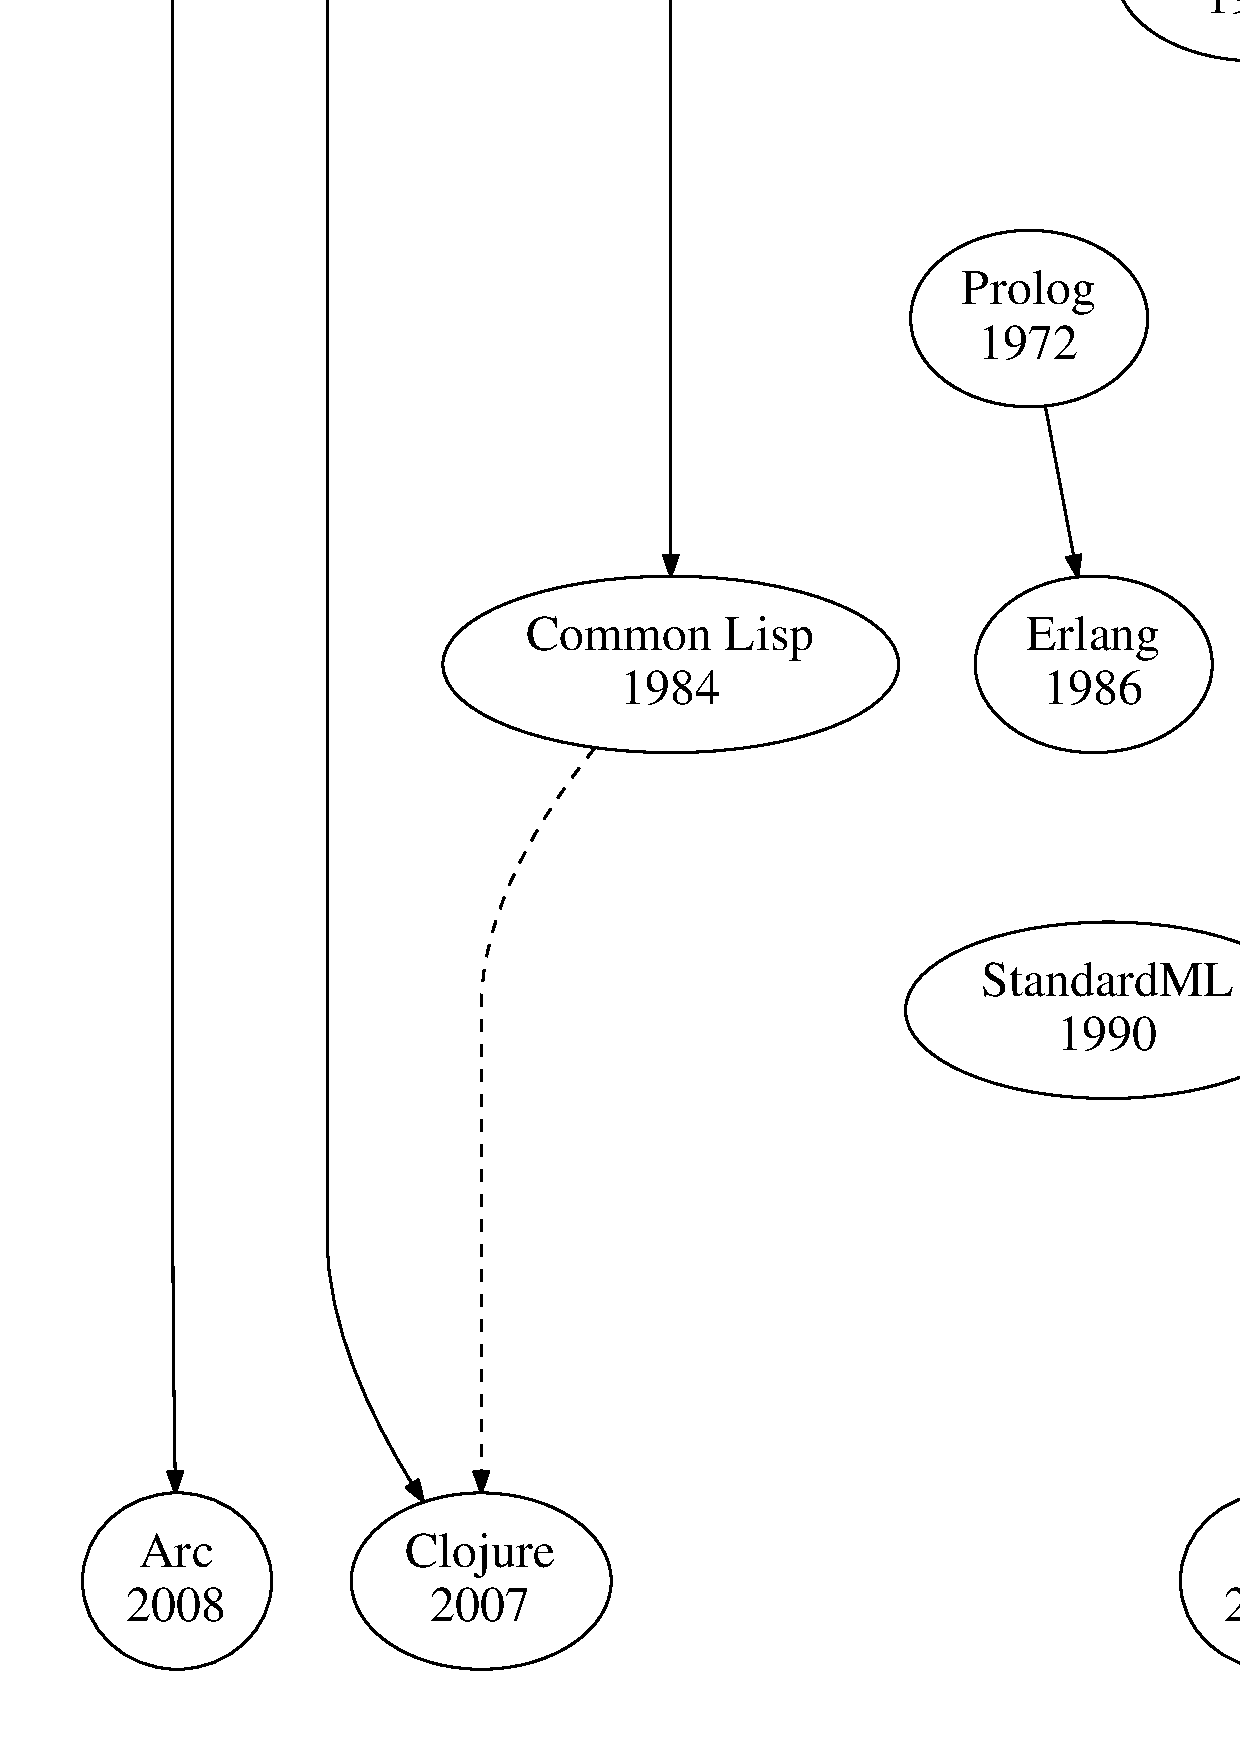
\includegraphics[width=\textwidth]{languages.pdf}
  \else
    \includegraphics[width=\textwidth]{languages.ps}
  \fi
\caption{Родословное древо функциональных языков}
\label{lineage}
\end{figure}

Как уже упоминалось в разделе \ref{benefits}, функциональные языки существуют довольно давно. Первый из них, Лисп, создан в 1958 году, всего на год позже первого императивного языка~--- Фортрана. Ещё один известный функциональный язык, РЕФАЛ, создан В.Ф.Турчиным в 1966 году. Но если РЕФАЛ стал широко известен довольно поздно (возможно, по причинам, далёким от программирования: он был создан в СССР в эпоху Холодной войны, а ФП развивалось в то время в основном по другую сторону Железного занавеса), то распространение Лиспа продолжалось всё время его существования. Уже в двухтысячных годах появились два новых популярных диалекта этого языка: Arc и Clojure.

Наиболее известные диалекты Лиспа~--- Common Lisp и Scheme. Первый чаще других вариантов Лиспа применяется на практике, а вторая используется в основном для обучения программированию. К сожалению, непоследовательная политика стандартизации сильно замедлила распространение Scheme как языка практического программирования.

Изучение Лиспа (скорее всего, Scheme) практически неизбежно для человека, интересущегося функциональным программированием, так как многие важные работы на эту тему используют именно Scheme в качестве языка примеров. Среди возможностей Scheme, отсутствующих в Эрланге, особенно интересны  продолжения (continuations)~--- способ сохранять как значение состояние программы в определённый момент.

Второй после Лиспа по влиятельности и многочисленности <<потомства>> функциональный язык это ML. В нём впервые была реализована очень мощная техника~--- {\em вывод типов}, то есть автоматическое определение компилятором типа выражения по контексту, в котором оно используется. Вывод типов избавляет программиста от целого класса неприятных ошибок. В этой книжке я использовал язык без вывода типов\footnote{На самом деле, похожие инструменты для Эрланга реализованы, но они гораздо слабее своих аналогов из языков-потомков ML.} только потому, что это сильно усложнило и удлинило бы курс.

Наиболее известные потомки ML это OCaml, F\# (построенный на базе OCaml язык для платформы .Net) и Haskell.

Именно Haskell считается <<передним краем>> исследований в области функционального программирования. В практическом программировании он применяется не так часто, возможно, потому, что его авторы очень жёстко отказываются вносить в язык полезные для индустрии, но <<некрасивые>> с точки зрения теории возможности~--- полушутливый девиз Haskell это <<Avoid success at all costs>> (<<Избегать успеха любой ценой>>). Пожалуй, Haskell~--- это второй после Scheme язык, изучения которого интересующемуся ФП человеку вряд ли удастся избежать. Изучить этот язык стоит хотя бы для того, чтобы познакомиться с такими интереснейшими концепциями, как ленивые вычисления или монады.

К сожалению, малопопулярен другой замечательный диалект ML~--- StandardML, очень красивый, гораздо более компактный, чем Haskell (и, на мой взгляд, более логичный синтаксически, чем OCaml и F\#) язык.

Ну и, наконец, не надо забывать, что Эрланг мы тоже изучили не до конца. Если вам понравился Эрланг, стоит всерьёз заняться изучением его возможностей. На самом деле, в этом курсе вообще не используется одно из главных преимуществ Эрланга~--- библиотека OTP, Open Telecom Platform, предоставляющая готовые решения для задач параллельного и распределённого программирования. <<За кадром>> остались также поведения (behaviours), обработка исключительных ситуаций, макросы и многое другое.

\section{Что ещё можно почитать про ФП}

Функциональному программированию посвящено довольно много книг, ресурсов в Интернете и журналов. Хорошей стартовой точкой для дальнейшего знакомства с миром ФП может стать журнал <<Практика функционального программирования>>, свободно доступный на сайте \url{http://fprog.ru/}. Кстати, в первом номере журнала опубликован обзор литературы по функциональному программированию, сделанный Алексеем Оттом~\cite{PFP_Ott}.

Ещё одна хорошая обзорная статья~--- <<Функциональное программирование для всех>> В.Ахмечета~\cite{Akhmechet}, опубликованная в журнале RSDN Magazine.

Среди книг прежде всего надо упомянуть <<Структуру и интерпретацию компьютерных программ>> Х.Абельсона и Дж.Сассмана~\cite{SICP}, которая по праву считается классической. Это учебник по программированию вообще, не только функциональному, но значительная часть материала изложена именно с помощью функциональных решений.

Большинство работ по алгоритмам и структурам данных расчитано на императивные языки. Эту ситуацию пытается исправить Крис Окасаки, автор книги <<Чисто функциональные структуры данных>>~\cite{Okasaki}. Ещё одна серьёзная работа по теоретическим аспектам программирования, ориентированная на ФП~--- <<Типы в языках программирования>> Б.Пирса~\cite{Pierce}.

Очень хороший пример практического программирования на функциональных языках приводится в статье Д.Астапова <<Давно не брал я в руки шашек>>~\cite{PFP_Astapov}. Интересующимся продвинутыми программистскими техниками будет, вероятно, интересно прочитать статьи А.Вознюка о продолжениях~\cite{PFP_Voznyuk} и И.Ключникова о суперкомпиляции~\cite{PFP_Klyuchnikov}. Впрочем, как уже говорилось, журнал <<Практика функционального программирования>>, в котором опубликованы все эти статьи, вообще рекомендуется к ознакомлению при наличии интереса к теме.

Замечательные учебники по языку Scheme и функциональному программированию~--- книги <<Little Schemer>>~\cite{little_schemer} и <<Seasoned Schemer>>~\cite{seasoned_schemer}, к сожалению, в отличие от SICP не переведены на русский язык.

Хороший вводный материал по языку Haskell~--- цикл статей Алексея Бешенова~\cite{Beshenov} и книга <<Изучай Haskell во имя добра!>>~\cite{Lipovacha}, а если говорить об источниках на английском языке~--- <<Real World Haskell>>~\cite{real_world_haskell}. По Стандартному ML на русском издана книга Р.Харпера <<Введение в Стандартный ML>>~\cite{Harper}.

Про возможности OTP, концепцию <<поведений>> (behaviours) можно прочитать в книге \cite{cesarini}. Из важных книг по Эрлангу, пока не переведённых на русский язык, надо упомянуть учебник Дж.Армстронга (создателя языка)~\cite{armstrong} и книгу <<Erlang and OTP in action>>~\cite{OTP_in_action}. Хороший вводный курс, правда, во многом дублирующий уже изложенное здесь~--- <<Learn You Some Erlang for Great Good>>~\cite{LYSE}.

\chapter*{Решения задач}
\addcontentsline{toc}{chapter}{Решения задач}
\markboth{Решения задач}{Азбука ФП}

\section*{Азбука ФП}
\addcontentsline{toc}{section}{Азбука ФП}

\solution{nand}

\lstinputlisting{abc/nand/logic.erl}

Вообще говоря, функцию \lstinline{nand} можно было бы определить гораздо проще:

\begin{lstlisting}
nand(true, true) -> false;
nand(_, _) -> true.
\end{lstlisting}

Но этот вариант функции \lstinline{nand} не будет выдавать ошибку, если передать ему в качестве аргументов что-то помимо атомов\index{Атом} \lstinline{true} и \lstinline{false}, что может затруднить поиск источника проблемы в неправильно написанной программе. Поэтому лучше перечислить все корректные варианты аргументов явно.

Помните, в Эрланге принят подход <<Let it fail>>~--- <<Пусть падает>>.

\solution{myor}

\lstinputlisting{abc/logic.erl}

\solution{author}

\lstinputlisting{abc/author.erl}

\solution{sign}

\lstinputlisting{abc/sign.erl}

\solution{divisor}

\lstinputlisting{abc/divisor.erl}

\solution{summ}

\lstinputlisting{abc/summ.erl}

\solution{divisors}

\lstinputlisting{abc/divisors.erl}

\solution{remainder}

\lstinputlisting{abc/remainder.erl}

\solution{number_sequence}

\lstinputlisting{abc/number_input.erl}

Эту задачу можно решить и иначе~--- например, вот так:

\lstinputlisting{abc/number_input/number_input.erl}

Идея решения та же самая, а как её оформить~--- вопрос вкуса. В таком варианте приодится дублировать оператор ввода, зато вместо \lstinline{case} используется сопоставление с образцом\index{Сопоставление с образцом}, что, по идее, должно делать код более понятным.

\solution{rember}

\lstinputlisting{abc/rember.erl}

\solution{listrev}

\lstinputlisting{abc/listrev.erl}

\solution{slice}

\lstinputlisting[language=erlang]{sugar/slice.erl}

\solution{flatten}

Алгоритм решения этой задачи можно коротко описать так: мы создаём временный список для хранения текущего разбираемого элемента (второй аргумент функции \lstinline{flatten/2}). Поначалу он пуст (это тот второй аргумент, который передаёт функции \lstinline{flatten/2} функция \lstinline{flatten/1}).

Если исходный список тоже пуст, то работа закончена (первый вариант функции).

Если исходный список не пуст, то мы берём его голову и помещаем во временный список для разбора (второе тело функции).

Если текущий разбираемый элемент это тоже список, то мы берём его голову, а хвост возвращаем в исходный список, где он будет дожидаться своей очереди (третье тело функции).

Наконец, если ни одно из предыдущих сопоставлений с образцом\index{Сопоставление с образцом} не увенчалось успехом, надо полагать, что хранилище разбираемых элементов не пусто (иначе бы сработали бы образцы 1 или 2) и то, что в нём лежит~--- не список (иначе сработал бы образец 3). Следовательно, это одиночное значение и мы можем смело помещать его в голову итогового списка.

\lstinputlisting{abc/flatten.erl}

\solution{palindrome}

\lstinputlisting[language=erlang]{best_practices/palindrome.erl}

\solution{perfect}
Функция \lstinline{divisors}, составляющая список делителей числа $N$, лежащих в интервале от 1 до $M$ включительно~--- это попросту индуктивное определение такого списка: если он заканчивается единицей, то только единица в него и войдёт, а если он должен состоять из чисел в интервале от единицы до некоего числа $M$, большего, чем единица, то в него войдут делители числа $N$ в интервале от 1 до $M-1$, а также само $M$, если оно тоже является делителем $N$.

Случай с единицей мы обрабатываем в \lstinline{divisors/1}, чтобы избежать лишнего вызова функции.

Функция \lstinline{lists:sum} из модуля \lstinline{lists}, подсчитывающая сумму списка чисел, ощутимо упрощает решение этой задачи.

Обратите внимание, что функция \lstinline{divisors} небезопасна и будет зацикливаться при значениях $M$ меньше 1. Здесь было разумным пожертвовать безопасностью в ущерб ясности; в реальных программах часто полезно делать наоборот.
\lstinputlisting[language=erlang]{abc/perfect.erl}
\pagebreak

\solution{brackets}
В этой задаче можно представлять строку для разбора либо как обычный эрланговский список, либо как битовую строку. Решение с битовыми строками чуть более громоздко, но в реальной жизни битовые строки гораздо полезнее <<строк>>, хранящихся как списки ASCII-кодов.

Алгоритм же в обоих решениях~--- один и тот же: сделаем стек, в который будем класть все открывающие скобки. Встречая закрывающую скобку, будем выпихивать со стека верхнее значение. Если тип закрывающей скобки из текущей позиции строки и открывающей скобки с вершины стека не совпали (или стек пуст), порядок скобок неправильный. Если после того, как вся строка разобрана, в стеке что-то осталось, порядок скобок тоже неправильный. Если же нам удалось подойти к концу строки с пустым стеком (или строка просто пустая), значит, порядок скобок~--- правильный.

\begin{figure}[!t,bracketspic]
\centerline{
\begin{pspicture}%[showgrid=true]
(10, 11)
\rput(2, 10.5){Входной список}
\rput(6.8, 10.5) {Стек}
\rput(0, 9){
  % Входной список
  \psgrid[gridlabels=0.0pt,subgriddiv=1](0,0)(0,0)(5,1)
  \rput(0.5, 0.5){[}
  \rput(1.5, 0.5){(}
  \rput(2.5, 0.5){<}
  \rput(3.5, 0.5){)}
  \rput(4.5, 0.5){]}
  % Операция
  \psbezier{->}(0.5,0)(0.5,-1)(6.5,0)(6.5,-1)
}
\rput(0, 7) {
  % Входной список
  \psgrid[gridlabels=0.0pt,subgriddiv=1](0,0)(0,0)(4,1)
  \rput(0.5, 0.5){(}
  \rput(1.5, 0.5){<}
  \rput(2.5, 0.5){)}
  \rput(3.5, 0.5){]}
  % Операция
  \psbezier{->}(0.5,0)(0.5,-1)(6.5,0)(6.5,-1)
  % Стек
  \psgrid[gridlabels=0.0pt,subgriddiv=1](0,0)(6,0)(7,1)
  \rput(6.5, 0.5){(}
}
\rput(0, 5) {
  % Входной список
  \psgrid[gridlabels=0.0pt,subgriddiv=1](0,0)(0,0)(3,1)
  \rput(0.5, 0.5){<}
  \rput(1.5, 0.5){)}
  \rput(2.5, 0.5){]}
  % Операция
  \psbezier{->}(0.5,0)(0.5,-1)(6.5,0)(6.5,-1)
  % Стек
  \psgrid[gridlabels=0.0pt,subgriddiv=1](0,0)(6,0)(8,1)
  \rput(6.5, 0.5){(}
  \rput(7.5, 0.5){[}
}
\rput(0, 3) {
  % Входной список
  \psgrid[gridlabels=0.0pt,subgriddiv=1](0,0)(0,0)(2,1)
  \rput(0.5, 0.5){)}
  \rput(1.5, 0.5){]}
  % Операция
  \psbezier{->}(0.5,0.0)(0.5,-1)(0.5,-1)(3.5,-1)
  \psbezier{->}(6.5,0.0)(6.5,-1)(6.5,-1)(4.5,-1)
  \rput(4, -1){\pscirclebox{?}}
  \psline{->}(4,-1.5)(4,-2)
  % Стек
  \psgrid[gridlabels=0.0pt,subgriddiv=1](0,0)(6,0)(9,1)
  \rput(6.5, 0.5){<}
  \rput(7.5, 0.5){(}
  \rput(8.5, 0.5){[}
  % Возвращаемое значение
  \rput(4, -2.5){false}
  \psbezier{->}(4.75,-2.5)(5.5,-3)(5.5,-2)(6.25,-2.5)
  \rput(7, -2.5){false}
}
\end{pspicture}
}
\caption{Функция \lstinline{is_valid_string/2} проверяет скобочную структуру <<[(<)]>> на правильность. Слева~--- входной список (первый аргумент функции), справа~--- стек (второй аргумент функции).}
\label{bracketspic}
\end{figure}

\lstinputlisting[language=erlang]{abc/brackets_str.erl}
\pagebreak
\lstinputlisting[language=erlang]{abc/brackets.erl}
\pagebreak

\solution{queue}

Идея решения вот в чём: реализуем очередь как два списка, входной и выходной. При помещении значения в очередь будем добавлять его в голову входного списка. При извлечении значения из очереди проверим, пуст ли выходной список. Если да, проверим, пуст ли входной. Если пуст и он, очередь пуста (второй вариант тела функции). А если входной список не пуст, развернём его, отдадим голову получившегося списка как выходное значение, а хвост поместим в выходной список (входной список, соответственно, становится пустым). Эти действия описаны в первом варианте тела функции. Ну а если выходной список не пуст, просто отдаём его голову, т.к. значения в нём уже стоят в правильном порядке (третий вариант тела функции).

Работа с организованной таким образом очередью будет выглядеть примерно так.

\begin{figure}[!t,queuepic]
\centerline{
\begin{pspicture}%[showgrid=true]
(9, 21)
\rput(3.0, 20.5){Входной}
\rput(3.0, 19.5){список}
\rput(6.0, 20.5){Выходной}
\rput(6.0, 19.5){список}
\rput(0, 18) {
  \psframe[linestyle=dotted](1.8,-0.2)(7.2, 1.2)
  % Операция
  \rput(0.5, 0.5){1}
  \psline{->}(0.8, 0.5)(1.6, 0.5)
}
\rput(0, 16) {
  \psframe[linestyle=dotted](1.8,-0.2)(7.2, 1.2)
  % Входной список
  \psgrid[gridlabels=0.0pt,subgriddiv=1](0,0)(2,0)(3,1)
  \rput(2.5, 0.5){1}
  % Операция
  \rput(0.5, 0.5){2}
  \psline{->}(0.8, 0.5)(1.6, 0.5)
}
\rput(0, 14) {
  \psframe[linestyle=dotted](1.8,-0.2)(7.2, 1.2)
  % Входной список
  \psgrid[gridlabels=0.0pt,subgriddiv=1](0,0)(2,0)(4,1)
  \rput(2.5, 0.5){2}
  \rput(3.5, 0.5){1}
  % Операция
  \rput(0.5, 0.5){3}
  \psline{->}(0.8, 0.5)(1.6, 0.5)
}
\rput(0, 12) {
  \psframe[linestyle=dotted](1.8,-0.2)(7.2, 1.2)
  % Операция
  \rput(8.5, 0.5){1}
  \psline{->}(7.4, 0.5)(8.2, 0.5)
  % Выходной список
  \psgrid[gridlabels=0.0pt,subgriddiv=1](0,0)(5,0)(7,1)
  \rput(5.5, 0.5){3}
  \rput(6.5, 0.5){2}
}
\rput(0, 10) {
  \psframe[linestyle=dotted](1.8,-0.2)(7.2, 1.2)
  % Операция
  \rput(0.5, 0.5){4}
  \psline{->}(0.8, 0.5)(1.6, 0.5)
  % Выходной список
  \psgrid[gridlabels=0.0pt,subgriddiv=1](0,0)(5,0)(7,1)
  \rput(5.5, 0.5){3}
  \rput(6.5, 0.5){2}
}
\rput(0, 8) {
  \psframe[linestyle=dotted](1.8,-0.2)(7.2, 1.2)
  % Входной список
  \psgrid[gridlabels=0.0pt,subgriddiv=1](0,0)(2,0)(3,1)
  \rput(2.5, 0.5){4}
  % Операция
  \rput(0.5, 0.5){5}
  \psline{->}(0.8, 0.5)(1.6, 0.5)
  % Выходной список
  \psgrid[gridlabels=0.0pt,subgriddiv=1](0,0)(5,0)(7,1)
  \rput(5.5, 0.5){3}
  \rput(6.5, 0.5){2}
}
\rput(0, 6) {
  \psframe[linestyle=dotted](1.8,-0.2)(7.2, 1.2)
  % Входной список
  \psgrid[gridlabels=0.0pt,subgriddiv=1](0,0)(2,0)(4,1)
  \rput(2.5, 0.5){5}
  \rput(3.5, 0.5){4}
  % Операция
  \rput(8.5, 0.5){2}
  \psline{->}(7.4, 0.5)(8.2, 0.5)
  % Выходной список
  \psgrid[gridlabels=0.0pt,subgriddiv=1](0,0)(6,0)(7,1)
  \rput(6.5, 0.5){3}
}
\rput(0, 4) {
  \psframe[linestyle=dotted](1.8,-0.2)(7.2, 1.2)
  % Входной список
  \psgrid[gridlabels=0.0pt,subgriddiv=1](0,0)(2,0)(4,1)
  \rput(2.5, 0.5){5}
  \rput(3.5, 0.5){4}
  % Операция
  \rput(8.5, 0.5){3}
  \psline{->}(7.4, 0.5)(8.2, 0.5)
}
\rput(0, 2) {
  \psframe[linestyle=dotted](1.8,-0.2)(7.2, 1.2)
  % Операция
  \rput(8.5, 0.5){4}
  \psline{->}(7.4, 0.5)(8.2, 0.5)
  % Выходной список
  \psgrid[gridlabels=0.0pt,subgriddiv=1](0,0)(6,0)(7,1)
  \rput(6.5, 0.5){5}
}
\rput(0, 0) {
  \psframe[linestyle=dotted](1.8,-0.2)(7.2, 1.2)
  % Операция
  \rput(8.5, 0.5){5}
  \psline{->}(7.4, 0.5)(8.2, 0.5)
}
\end{pspicture}
}
\caption{Организация очереди из двух списков.}
\label{queuepic}
\end{figure}

Компилируем модуль, загружаем определение записи:
\erlshell{c(listqueue).}{\{ok,listqueue\}}
\erlshell{rr("queue.hrl").}{{[}queue{]}}

Создаём новую очередь:
\erlshell{Q1 = \#queue\{\}.}{\#queue\{in = [],out = []\}}

Помещаем в очередь значение 1:
\erlshell{Q2 = listqueue:enqueue(Q1, 1).}{\#queue\{in = [1],out = []\}}

Помещаем в очередь значение 2:
\erlshell{Q3 = listqueue:enqueue(Q2, 2).}{\#queue\{in = [2,1],out = []\}}

Помещаем в очередь значение 3:
\erlshell{Q4 = listqueue:enqueue(Q3, 3).}{\#queue\{in = [3,2,1],out = []\}}

Извлекаем из очереди первое значение (1)~--- в этот момент входной список будет развёрнут и перемещён в выходной:
\erlshell{\{ok, Out1, Q5\} = listqueue:dequeue(Q4).}{\{ok,1,\#queue\{in = [],out = [2,3]\}\}}
\erlshell{Out1.}{1}

Добавляем в очередь значение 4 (с этого момента формируется новый входной список):
\erlshell{Q6 = listqueue:enqueue(Q5, 4).}{\#queue\{in = [4],out = [2,3]\}}

Добавляем в очередь значение 5:
\erlshell{Q7 = listqueue:enqueue(Q6, 5).}{\#queue\{in = [5,4],out = [2,3]\}}

Извлекаем из очереди второе значение (2):
\erlshell{\{ok, Out2, Q8\} = listqueue:dequeue(Q7).}{\{ok,2,\#queue\{in = [5,4],out = [3]\}\}}

Извлекаем из очереди третье значение (3):
\erlshell{\{ok, Out3, Q9\} = listqueue:dequeue(Q8).}{\{ok,3,\#queue\{in = [5,4],out = []\}\}}

Извлекаем из очереди четвёртое значение (4)~--- выходной список пуст, снова разворачиваем входной список и перемещаем его на место опустевшего выходного:
\erlshell{\{ok, Out4, Q10\} = listqueue:dequeue(Q9).}{\{ok,4,\#queue\{in = [],out = [5]\}\}}

Извлекаем из очереди пятое значение (5):
\erlshell{\{ok, Out5, Q11\} = listqueue:dequeue(Q10).}{\{ok,5,\#queue\{in = [],out = []\}\}}

Очередь пуста, при попытке извлечения дальнейших значений будет возвращена информация об ошибке:
\erlshell{listqueue:dequeue(Q11).}{\{error,"Queue is empty"\}}

Несмотря на наличие в этом алгоритме <<тяжёлой>> операции разворачивания списка, требующей $N$ шагов для списка из $N$ элементов, условиям задачи он отвечает, т.к. каждый проходящий через очередь элемент участвует в этой операции только один раз.

\lstinputlisting[language=erlang]{abc/listqueue.erl}

\solution{node_cut}

Обратите внимание на то, как функции \lstinline{trim/2} и \lstinline{trim/3} рекурсивно вызывают друг друга. Это полезный приём, который позволяет упростить отладку и тестирование, а также улучшить читаемость кода за счёт избавления от громоздких операторов ветвления.

\lstinputlisting[language=erlang]{abc/trimtree.erl}

\solution{node_count}

\lstinputlisting[language=erlang]{abc/treemeter.erl}

\section*{Полезные приёмы}
\addcontentsline{toc}{section}{Полезные приёмы}
\markright{Полезные приёмы}

\solution{already}

Хвостовая рекурсия уже используется в решениях задач \ref{summ}, \ref{divisors}, \ref{remainder}, \ref{listrev}, \ref{brackets}.

\solution{tail}

Функцию \lstinline{rember/2} из задачи \ref{rember} можно переписать следующим образом:

\lstinputlisting[language=erlang]{abc/tailrember.erl}

Проблема в том, что такой способ обработки списка разворачивает его, и нам приходится вызывать \lstinline{lists:reverse}, чтобы вернуть исходный порядок следования элементов. Поэтому применение здесь хвостовой рекурсии не очень оправдано. В решениях других задач применение хвостовой рекурсии принесёт ещё больше сложностей.

Не надо применять хвостовую рекурсию по любому поводу. Во-первых, она не всегда эффективнее обычной, во-вторых, помните: сначала стабильная работа программы, потом оптимизация.

\solution{perfect_list}

\lstinputlisting[language=erlang]{best_practices/perfect.erl}
\pagebreak

\solution{maptree}

\lstinputlisting[language=erlang]{best_practices/maptree.erl}

\solution{length}
\begin{lstlisting}
lists:foldl(fun(_, Length) -> Length + 1 end, 0, L).
\end{lstlisting}

\solution{foldrev}

\lstinputlisting[language=erlang]{best_practices/foldrev.erl}

\solution{mean}

\lstinputlisting[language=erlang]{best_practices/mean.erl}

\solution{foldl1}

\lstinputlisting[language=erlang]{best_practices/mylists.erl}

\solution{foldseq}

\lstinputlisting[language=erlang]{best_practices/myseq.erl}

\solution{ismemberof}

\lstinputlisting[language=erlang]{best_practices/ismemberof.erl}

\section*{Приятные мелочи}
\addcontentsline{toc}{section}{Приятные мелочи}
\markright{Приятные мелочи}

\solution{short_perfect}

\lstinputlisting[language=erlang]{sugar/perfect.erl}

\solution{common}

\lstinputlisting[language=erlang]{sugar/common_members.erl}

\solution{multiplication}

\lstinputlisting[language=erlang]{best_practices/multiplication.erl}

\solution{common_without_member}

\lstinputlisting[language=erlang]{sugar/common2.erl}

\solution{queens}

\lstinputlisting[language=erlang]{sugar/queens.erl}

%% Решение из статьи про задачу в Википедии %% (http://ru.wikipedia.org/wiki/%D0%97%D0%B0%D0%B4%D0%B0%D1%87%D0%B0_%D0%BE_%D0%B2%D0%BE%D1%81%D1%8C%D0%BC%D0%B8_%D1%84%D0%B5%D1%80%D0%B7%D1%8F%D1%85#.D0.A0.D0.B5.D0.B0.D0.BB.D0.B8.D0.B7.D0.B0.D1.86.D0.B8.D1.8F_.D0.BD.D0.B0_Erlang):

%% pmut([])->
%%         [[]];
%% pmut(A) ->
%%         [[H|T] || H <- A, T <- pmut(A--[H])].
 
%% start() ->
%%         N = 8, % size of board / num of queens (N>=4)
%%         ListP = pmut(lists:seq(1,N)),
%%         [Q || Q <- ListP, length(lists:usort([lists:nth(X,Q)+X || X <- %% Q])) == N, 
%%         length(lists:usort([lists:nth(X,Q)-X || X <- Q])) == N]

\solution{foldrrev}

\lstinputlisting[language=erlang]{sugar/foldrrev.erl}

\solution{linearize}

\lstinputlisting[language=erlang]{sugar/trees-linearize/trees.erl}

\solution{hanoi}

Сформулируем принципы перекладывания стопки из $N$ дисков.

Базовый случай в этой задаче~--- $N=0$, т.е. ситуация, когда нам ничего перекладывать не нужно. Большее количество дисков перекладывается по следующему алгоритму (стержень, с которого перемещаем диски, будем называть исходным, стержень, на который перемещаем диски~--- целевым, а третий~--- вспомогательным):

\begin{enumerate}
\item Взять $N-1$ дисков и переместить их с исходного стержня на вспомогательный.
\item Переместить оставшийся на исходном стержне диск на целевой стержень.
\item Переместить $N-1$ дисков со вспомогательного стержня на целевой.
\end{enumerate}

Первый и третий шаги предполагают перекладывание стопки дисков, то есть рекурсивный вызов процедуры перекладывания. Но так как в каждом следующем вызове $N$ гарантированно уменьшается, мы можем быть уверены, что рано или поздно рекурсия закончится.

\lstinputlisting[language=erlang]{sugar/hanoi.erl}

\solution{dropwhile}

Сложность с реализацией \lstinline{dropwhile} в том, что реакция на элемент, для которого переданная функция возвращает \lstinline{true}, должна отличаться в зависимости от того, встретился ли нам уже элемент, для которого эта функция вернула \lstinline{false}. Так как мы имеем дело со свёрткой\index{Свёртка списка}, мы не можем ввести какой-то дополнительный параметр, указывающий, так ли это~--- ведь тогда свёртка вернёт его вместе с итоговым списком, а это не то, что нам нужно.

Но на самом деле при левой свёртке\index{Свёртка списка!левая} таким параметром является сам итоговый список: если он пуст, значит, не отвечающий критерию элемент нам ещё не встречался и мы должны проверить текущий элемент с помощью функции-аргумента. Если список не пуст, мы должны безо всяких проверок поместить в него текущий элемент.

\lstinputlisting[language=erlang]{best_practices/dropwhile.erl}

Реализовать \lstinline{dropwhile} с помощью правой свёртки\index{Свёртка списка!правая}, строго говоря, невозможно~--- правая свёртка начинается с конца списка, что не позволяет нам найти первое с начала списка вхождение элемента с её помощью. Но динамическая типизация Эрланга позволяет нам реализовать обходное решение, жульническое по сути (реальная работа делается вне свёртки), но позволяющее <<обмануть>> функцию \lstinline{foldr}, подсунув ей функцию, которая формально удовлетворяет условиям задачи:

\lstinputlisting[language=erlang]{best_practices/rdropwhile.erl}

Идея этого решения в следующем: мы заранее находим первый элемент в списке, для которого функция \lstinline{F} вернёт \lstinline{false} и запоминаем его позицию (далее будем называть её <<линией отреза>>. После этого мы определяем функцию \lstinline{Trim}, у которой есть два варианта списка аргументов: либо текущий элемент списка и кортеж вида {\em \{Накопленный хвост списка, Позиция текущего элемента, Линия отреза\}}, либо текущий элемент и список.

\lstinline{Trim} будет добавлять к накопленному хвосту списка элемент за элементом, пока позиция текущего элемента не совпадёт с линией отреза. В этот момент она оставит в аргументе-накопителе только список. Следующие вызовы, обнаружив во втором аргументе список вместо кортежа, просто передадут аргумент-накопитель дальше.

Обратите внимание, что ситуация, когда элемент, для которого \lstinline{F} возвращает \lstinline{false}, так и не был найден, требует особой обработки.

Надо ещё раз подчеркнуть, что это решение является хаком в самом плохом смысле этого слова и непереносимо на многие функциональные языки с более строгим контролем типов, вроде Стандартного ML и Haskell (решения, построенные на аналогичной идее, пожалуй, возможны и там, но ценой ещё более уродливых ухищрений).

\solution{permutations}

Идея решения этой задачи вот в чём. В список перестановок списка длины $1$ входит единственный элемент~--- он сам. А перестановки списка большей длины можно получить так: по очереди удалять из списка каждый элемент, получать все перестановки оставшихся и в начало каждой из них подставлять удалённый элемент.

% Я видел где-то лучшее решение с --

\lstinputlisting[language=erlang]{sugar/permutations.erl}

\section*{От функционального программирования к параллельному}
\addcontentsline{toc}{section}{От функционального программирования к параллельному}
\markright{От ФП к ПП}

\solution{approximation}

\lstinputlisting[language=erlang]{parallel/montecarlo.erl}

\solution{fibmem}

\lstinputlisting[language=erlang]{parallel/fibmem.erl}

% Приложение: отладчик, запускающийся по debugger:start()? Трассировщик, если он может быть чем-то полезен? EUnit?

% Приложение: установка Эрланга на разных платформах?

\addcontentsline{toc}{chapter}{Литература}
\begin{thebibliography}{99}
\bibitem[Абельсон 2010]{SICP}
Абельсон Х., Сассман Дж. Дж. Структура и интерпретация компьютерных программ. М.: <<Добросвет>>, <<КДУ>>, 2010.
\bibitem[Астапов 2009]{PFP_Astapov}
Астапов Д. Давно не брал я в руки шашек // Практика функционального программирования, №1, 2009.
\bibitem[Ахмечет 2006]{Akhmechet}
Ахмечет В. Функциональное программирование для всех. // RSDN Magazine, №2, 2006.
\bibitem[Бешенов 2010]{Beshenov}
Бешенов А. Функциональное программирование на Haskell.\\
\href{http://www.ibm.com/developerworks/ru/library/l-haskell/}{Часть 1. Введение.}\\
\href{http://www.ibm.com/developerworks/ru/library/l-haskell2/}{Часть 2.Основные типы и классы.}\\
\href{http://www.ibm.com/developerworks/ru/library/l-haskell3/}{Часть 3. Определение функций.}\\
\href{http://www.ibm.com/developerworks/ru/library/l-haskell4/}{Часть 4. Свертки списков.}
\bibitem[Вознюк 2011]{PFP_Voznyuk}
Вознюк А. Продолжения в практике. // Практика функционального программирования, №7, 2011.
\bibitem[Златопольский 2007]{zlatopolsky}
Златопольский Д.М. Программирование: типовые задачи, алгоритмы, методы. М., 2007.
\bibitem[Ключников 2011]{PFP_Klyuchnikov}
Ключников И. Суперкомпиляция: идеи и методы. // Практика функционального программирования, №7, 2011.
\bibitem[Липовача 2012]{Lipovacha}
Липовача М. Изучай Haskell во имя добра! М.: <<ДМК Пресс>>, 2012.
\bibitem[Отт 2009]{PFP_Ott}
Отт А. Обзор литературы о функциональном программировании. // Практика функционального программирования, №1, 2009.
\bibitem[Пирс 2012]{Pierce}
Пирс Б., Типы в языках программирования. М.: <<Лямбда пресс>>, <<Добросвет>>, 2012.
\bibitem[Харпер 1996]{Harper}
Харпер Р. Введение в Стандартный ML. М., 1996.
\bibitem[Чезарини 2012]{cesarini}
Чезарини Ф., Томпсон С. Программирование в Эрланг. М.: <<ДМК Пресс>>,
2012.
\bibitem[Шень 2004]{shen}
Шень А. Программирование: теоремы и задачи. М.: МЦНМО, 2004.
\bibitem[99 problems]{99problems}
99 Problems на выбранном языке (точно есть для \href{http://www.haskell.org/haskellwiki/99_questions}{Haskell}, \href{http://aperiodic.net/phil/scala/s-99/}{Scala}, \href{https://sites.google.com/site/prologsite/prolog-problems}{Prolog}, \href{http://www.christiankissig.de/cms/index.php/en/programming/28-ocaml/28-99-problems-in-ocaml}{OCaml}, \href{http://www.informatimago.com/develop/lisp/l99/index.html}{Common Lisp}).
\bibitem[Armstrong 2007]{armstrong}
Armstrong J. Programming Erlang: Software for a Concurrent World. Pragmatic Bookshelf, 2007.
\bibitem[Friedman 1996]{little_schemer}
Friedman D.P., Fellsen M. The Little Schemer. MIT Press, 1996.
\bibitem[Friedman 1996,2]{seasoned_schemer}
Friedman D.P., Fellsen M. The Seasoned Schemer. MIT Press, 1996.
\bibitem[LYSE]{LYSE}
Learn You Some Erlang for Great Good, \url{http://learnyousomeerlang.com/}.
\bibitem[Logan 2011]{OTP_in_action}
Logan M., Merritt E., Carlsson R. Erlang and OTP in action. Manning Publications, 2011.
\bibitem[Miller]{miller}
Evan Miller. The Joy of Erlang; Or, How To Ride A Toruk, \url{http://www.evanmiller.org/joy-of-erlang.html}.
\bibitem[Okasaki 1999]{Okasaki}
Okasaki C. Purely Functional Data Structures. Cambridge University Press, 1999.
\bibitem[O'Sullivan 2008]{real_world_haskell}
O'Sullivan B., Goerzen J., D.B. Stewart. Real World Haskell. Code You Can Believe In. O'Reilly, 2008.
\end{thebibliography}

\appendix

\pagebreak
\addcontentsline{toc}{chapter}{Приложения}

\chapter{Краткий справочник по используемым функциям}

\section*{Ввод-вывод}
\addcontentsline{toc}{section}{Ввод-вывод}
\markright{Ввод-вывод}

Здесь приводятся только те функции, которые требуются для той или иной задачи. С полной документацией на упомянутые модули можно ознакомиться на сайте языка: \url{http://erlang.org/doc/}.

\begin{funcdescr}
\funcdoc{io:format/1}{Принимает строку с командами формата и выводит её на экран.}
\funcdoc{io:format/2}{Принимает строку с командами формата и список подставляемых значений; выводит на экран строку, в которую подставлены значения в соответствии с командами формата.}
\funcdoc{io:fread/2}{Принимает подсказку и строку формата; читает со стандартного ввода выражения и пытается привести их к типам, заданным строкой формата; в случае успеха возвращает кортеж из атома \lstinline{ok} и списка прочитанных значений, в случае  ошибки~--- кортеж из атома \lstinline{error} и описания ошибки.}
\funcdoc{io:read/1}{Принимает подсказку для ввода; читает со стандартного ввода выражение Эрланга и возвращает кортеж из атома \lstinline{ok} и прочитанного выражения в случае успеха либо кортеж из атома \lstinline{error} и описания ошибки в случае ошибки.}
\end{funcdescr}

\section*{Математика}
\addcontentsline{toc}{section}{Математика}
\markright{Математика}

\begin{funcdescr}
\funcdoc{abs/1}{Возвращает модуль числа.}
\funcdoc{math:sqrt/1}{Возвращает квадратный корень своего аргумента.}
\funcdoc{random:uniform/0}{Возвращает случайное вещественное число в интервале от 0.0 до 1.0.}
\funcdoc{random:uniform/1}{Возвращает случайное целое число в интервале от 1 до своего аргумента.}
\end{funcdescr}

\section*{Обработка списков}
\addcontentsline{toc}{section}{Обработка списков}
\markright{Обработка списков}

\begin{funcdescr}
\funcdoc{length/1}{Принимает список; возвращает длину этого списка.}
\funcdoc{lists:dropwhile/2}{Принимает функцию-тест и список; возвращает список, из которого выброшены все элементы до первого, для которого функция-тест вернула \lstinline{false}.}
\funcdoc{lists:filter/2}{Принимает функцию-тест и список; возвращает список, в котором оставлены только те элементы, для которых функция-тест вернула \lstinline{true}.}
\funcdoc{lists:foldl/3}{Левая свёртка: принимает функцию, начальное значение накопителя и список. Функция-аргумент должна принимать два параметра: текущее значение накопителя и текущий элемент списка, а возвращать новое значение накопителя. Применяет функцию-аргумент ко всем элементам списка слева направо (от первого до последнего). Возвращает итоговое значение накопителя.}
\funcdoc{lists:foldr/3}{Правая свёртка: принимает функцию, начальное значение накопителя и список. Функция-аргумент должна принимать два параметра: текущее значение накопителя и текущий элемент списка, а возвращать новое значение накопителя. Применяет функцию-аргумент ко всем элементам списка cправа налево (от последнего до первого). Возвращает итоговое значение накопителя.}
\funcdoc{lists:map/2}{Принимает функцию от одного аргумента и список; возвращает список результатов применения переданной функции к элементам списка.}
\funcdoc{lists:max/1}{Принимает список; возвращает самый большой элемент списка.}
\funcdoc{lists:member/2}{Принимает значение и список; возвращает \lstinline{true}, если значение содержится в списке, и \lstinline{false}, если нет.}
\funcdoc{lists:reverse/1}{Принимает список; возвращает список, элементы которого идут в обратном относительно исходного списка порядке.}
\funcdoc{lists:seq/2}{Принимает два целых числа; возвращает идущие подряд целые числа от первого до второго аргумента включительно.}
\funcdoc{lists:sort/1}{Принимает список; возвращает список с элементами исходного списка, отсортированными по возрастанию.}
\funcdoc{lists:sort/2}{Принимает функцию сравнения и список;   возвращает список, отсортированный по возрастанию в соответствии с функцией сравнения. Функция сравнения должна принимать два аргумента и возвращать \lstinline{true}, если первый аргумент меньше второго или равен ему, и \lstinline{false} в противном случае.}
\funcdoc{lists:sum/1}{Принимает список чисел; возвращает сумму его элементов.}
\end{funcdescr}

\section*{Структуры данных}
\addcontentsline{toc}{section}{Структуры данных}
\markright{Структуры данных}

\begin{funcdescr}
\funcdoc{dict:new/0}{Возвращает пустой словарь.}
\funcdoc{dict:append/3}{Принимает ключ, значение и словарь; возвращает новый словарь, в котором к значениям по переданному ключу добавилось переданное значение.}
\funcdoc{dict:find/2}{Принимает ключ и словарь. Если в словаре содержатся значения по этому ключу, возвращает кортеж \lstinline{\{ok, Values\}}, где \lstinline{Values}~--- список найденных значений; в противном случае возвращает атом \lstinline{error}.}
\end{funcdescr}

\section*{Служебные функции Эрланга}
\addcontentsline{toc}{section}{Служебные функции Эрланга}
\markright{Служебные функции Эрланга}

\begin{funcdescr}
\funcdoc{register/2}{Принимает атом и идентификатор процесса; если атом ещё не используется в качестве имени процесса, регистрирует процесс под этим именем и возвращает \lstinline{true}.}
\funcdoc{self/0}{Возвращает идентификатор процесса, из которого вызвана.}
\funcdoc{spawn/1}{Принимает функцию; запускает её в отдельном процессе и возвращает идентификатор этого процесса.}
\funcdoc{timer:tc/3}{Принимает имя модуля, имя функции и список аргументов; возвращает время в микросекундах, затраченное на вычисление переданной функции от переданных аргументов.}
\end{funcdescr}

\chapter{Команды формата}

\section*{Вывод}
\addcontentsline{toc}{section}{Вывод}
\markright{Вывод}

\renewcommand{\arraystretch}{1.5}
\begin{longtabu} to \linewidth {|X|X[2.8]|}
  \hline
  \lstinline{s} & Вывести строку.\\
  \hline
  \lstinline{w} & Вывести выражение Эрланга.\\
  \hline
  \lstinline{p} & Вывести выражение Эрланга с аккуратными переносами длинных строк и отступами. По умолчанию считает строку равной 80 символам. Принимает аргумент, задающий длину строки: так, команда формата <<{\tt \textasciitilde{}62p}>> будет считать длину строки равной 62 символам.\vspace{1ex}\\
  \hline
  \lstinline{B} & Вывести число в заданной системе счисления с основанием от 2 до 36, по умолчанию используется основание 10.\vspace{1ex}\\
  \hline
  \lstinline{n} & Перейти на новую строку.\\
  \hline
\end{longtabu}

\section*{Ввод}
\addcontentsline{toc}{section}{Ввод}
\markright{Ввод}

\begin{longtabu} to \linewidth {|X|X[2.8]|}
  \hline
  \lstinline{d} & Прочитать десятичное целое.\\
  \hline
  \lstinline{f} & Прочитать вещественное число.\\
  \hline
  \lstinline{s} & Прочитать строку. Принимает числовой аргумент~--- ограничение длины строки. Также принимает аргумент \lstinline{t}, включающий поддержку символов Unicode (нужно, если вы собираетесь вводить, например, русские буквы).\vspace{1ex}\\
  \hline
\end{longtabu}

Здесь приведены не все команды формата. Полное описание можно прочитать в документации модуля \lstinline{io} (\url{http://erlang.org/doc/man/io.html}).

% Предметный указатель
\pagebreak % Это хак, не знаю, как ещё его научить ставить правильную страницу.
\addcontentsline{toc}{chapter}{Предметный указатель}
\documentclass[
  paper=a4,
  fontsize=14pt,
  openany,
  appendixprefix=true
]{scrbook}
\usepackage{quicktour}
\author{Ю.А.Широков}
\title{Короткая экскурсия в функциональное программирование}
\begin{document}

\maketitle

\tableofcontents

\chapter*{От автора}
\addcontentsline{toc}{chapter}{От автора}
\markboth{От автора}{От автора}

Эта книга появилась практически случайно. Началось всё с разговоров о функциональном программировании с коллегами. В этих разговорах мне очень не хватало простых и понятных объяснений, в чём именно состоит функциональный подход. После нескольких таких бесед мне показалось, что я научился описывать функциональное программирование просто и при этом достаточно точно. Чтобы не забыть получившиеся формулировки, я решил записать их в виде короткого коспекта.

Конспект получился не таким уж коротким. Когда я его закончил, мне стало обидно, что несколько часов моего времени ушли на текст, который прочитаю только я сам. Поэтому, как только мне предоставился случай, я сказал нескольким знакомым, что с удовольствием бы прочитал вводную лекцию по функциональному программированию каким-нибудь студентам или продвинутым старшим школьникам.

Среди этих нескольких знакомых оказался Александр Трусевич, который предложил мне провести курс по функциональному программированию в физическом отделении Летней Экологической Школы (ЛЭШ). Не представляя себе, во что ввязываюсь, я согласился.

Быстро выяснилось, что конспект, которым я так гордился, никуда не годится~--- он полон непонятных школьникам терминов, зануден и слишком абстрактен. Пришлось писать с нуля новый рассказ о функциональном программировании (ставший в этой книге первой главой). Кроме того, пришлось заняться подбором задач. Эти-то задачи вместе с короткими объяснениями приёмов, применяемых для их решения, и стали в конце концов главным содержанием книги.

Сделать полноценный курс за лето 2012 года я не успел. Впрочем, и на ЛЭШ не попал. А к следующему лету курс увеличился насколько, что вываливать его весь на школьников ЛЭШ за пять дней было бы негуманно. И мне снова пришлось думать, в какой форме организовать свои заметки, чтобы работа не пропала зря.

Я хочу поблагодарить всех причастных к проведению ЛЭШ, её физического отделения и, конечно же, в особенности тех, кто слушал мой курс, а также героическую команду организаторов. Отдельное спасибо Александру Трусевичу, которому принадлежала сама исходная идея курса.

Разумеется, большинство приведённых в книге задач придумал не я. Все задачи, для которых удалось отыскать источник, снабжены ссылками на эти источники. Вклад авторов этих замечательных задач в книгу~--- никак не меньше моего.

Я вряд ли бы взялся оформить свои заметки в виде книги без вдохновляющего примера Георгия Бронникова, переведшего на русский язык три важнейших работы по функциональному программированию (\cite{SICP}, \cite{Pierce}, \cite{Okasaki}). Без книжки Сергея Львовского <<Набор и вёрстка в системе \LaTeX>> я не смог бы эти заметки оформить.

Анна Белякова, Татьяна Трошина и Алексей Туманов протестировали исходный набор задач и нашли в нём огромное количество опечаток, неточностей и ошибок. Кроме того, они указали мне множество плохо изложенных и непонятных мест в исходном варианте текста.

Последнее по порядку, но не по значению: моя жена, Катерина Шананина, проверила (и кое-где подправила) математические и околоматематические рассуждения, протестировала некоторые задачи и указала на множество неудачно сформулированных мест. Кроме того, именно она много лет назад убедила меня попробовать писать на языке LISP, познакомив с функциональным программированием.

Спасибо!

\chapter{Зачем нужно функциональное программирование}

\epigraph{Программы должны писаться для того,чтобы их читали люди, и только во вторую очередь для выполнения машиной.}{Х.Абельсон, Дж.Дж.Сассман}

\section{В погоне за ясностью}

Понимаем ли мы программы, которые пишем?

Если речь о маленьких программах, решающих не слишком сложные задачи, то обычно понимаем, конечно. Чтобы сделать непонятной простую программу, надо специально постараться. Кстати, некоторые и стараются~--- есть даже специальные шуточные языки программирования, на которых самые нехитрые программы тяжело писать и тем более читать. Например, brainfuck, на котором программа, выводящая на экран строку <<Hello, world!>>, выглядит так:
\begin{verbatim}
+++++ +++++
[
    > +++++ ++
    > +++++ +++++
    > +++
    > +
    <<<< -
]
> ++ .
> + .
+++++ ++ .
.
+++ .
> ++ .
<< +++++ +++++ +++++ .
> .
+++ .
----- - .
----- --- .
> + .
> .
\end{verbatim}

Или whitespace, в котором конструкции языка записываются невидимыми символами (пробел, табуляция, перевод строки), а все видимые символы используются только для комментариев.

Но с большими задачами человеку становится уже не до шуток. Грустно, но у нашего мозга много ограничений, здорово мешающих при занятиях математикой и программированием. Например, кратковременная память среднего человека может удерживать только около семи однотипных вещей (психологи называют это ограничение <<кошелёк Миллера>>).

Поэтому большую программу приходится писать по кусочкам. Чем больше эти кусочки, чем сильнее они связаны друг с другом, тем проще запутаться и ошибиться. На самом деле, даже самые лучшие программисты часто делают ошибки в программах, которые они пишут.

Чтобы найти уже существующие ошибки и не наделать новых, дописывая программу, программист должен прочитать её код и понять, что он делает. Потому что даже если он сам писал эту программу, то, как именно устроен каждый её кусок, он довольно быстро забывает. А уж если программу пишут вместе несколько программистов, то каждому обычно приходится сначала довольно долго читать чужой код, и только потом дописывать к нему свой.

Можно, конечно, попробовать упростить будущим читателям программы работу, написав комментарии. Вот только часто, поправив программу, поправить комментарии забывают, и они только сбивают с толку. А ведь ещё бывают случаи, когда комментарий с самого начала был неверен!

Поэтому язык программирования должен быть таким, чтобы программа легко читалась.

\important{Транслятор~--- программа, переводящая текст на языке программирования в машинные команды.}

Люди начали пытаться сделать языки программирования выразительными и простыми для чтения сразу же, как только мощность компьютеров позволила писать трансляторы для таких языков. Ещё в конце 1960-х годов Эдсгер Дейкстра предложил отказаться от оператора GOTO (переход на метку), чтобы сделать структуру программ понятнее.

\begin{figure}[!t,goto]

\includegraphics[width=180mm]{goto_russian.ps}
\caption{Использование GOTO опасно (\url{http://xkcd.com/292/}, русский перевод с \url{http://xkcd.ru/292/}).}
\label{goto}
\end{figure}

Дело в том, что от возможности <<прыгнуть>> в любое место программы из любого другого больше вреда, чем пользы. Пользуясь этой возможностью, можно создать программу, про которую будет очень тяжело понять, как она работает, да и последствия её работы могут быть непредсказуемыми (см. рис. \ref{goto}).

Дейкстра и его единомышленники призывали использовать в программах только последовательное исполнение, циклы (операторы \lstinline{for}, \lstinline{while} и т.п.), ветвление (операторы \lstinline{if}, \lstinline{case}) и вызовы функций. Такой стиль назвали <<структурным программированием>>, потому что он помогал сделать наглядной структуру программы.

Некоторое время даже достаточно большую по тогдашним меркам программу можно было сохранить понятной, соблюдая правила структурного стиля.

Но компьютеры становились мощнее, программы для них~--- больше, и правил структурного программирования стало недостаточно. Тогда программисты начали выдумывать новые способы сохранить программы понятными.

Некоторые из этих способов оказались не слишком удачными, как, например, попытка приблизить язык программирования к человеческому языку. Результат этой попытки, Кобол, оказался многословным и не слишком выразительным. (К сожалению, к моменту, когда это стало всем ясно, на Коболе уже написали огромное количество программ, и некоторые из них используются даже сейчас.)

Другие идеи сработали. Например, идея авторов языков Симула и Smalltalk: разделить код программы на кусочки, работающие с какой-то одной структурой данных, и разрешить этим кусочкам общаться между собой только с помощью чётко оговоренного набора сообщений. Тогда каждый такой кусочек можно переделывать как угодно, не беспокоясь, что сломаешь что-то в других частях программы~--- главное, чтобы его ответы на сообщения снаружи оставались такими же, как были.

% Пришлось изменить tolerance и emergencystretch, иначе LaTeX отказывался разрывать слова в кавычках
{\tolerance=100\emergencystretch=15pt Такие кусочки стали называть <<объектами>>, а стиль программирования, при котором программа так устроена~--- <<объектно-ори\-ен\-ти\-ро\-ван\-ным прог\-рам\-ми\-ро\-ва\-ни\-ем (ООП)>>.

}
Объектно-ориентированное программирование сильно упростило программистам жизнь, и в 1980-е, а особенно~--- в 1990-е годы очень многие программисты перешли на объектно-ориентированные языки. Но со временем стало ясно, что такие языки хорошо подходят не для всех задач. Кроме того, компьютеры стали ещё мощнее, программы~--- ещё больше, и программистам захотелось найти ещё какие-нибудь способы увеличить выразительность языков программирования.

\section{Выгоды функционального программирования}
\label{benefits}

Функциональное программирование (часто для краткости пишут просто ФП)~--- один из способов сделать код коротким и понятным одновременно. Есть у него и другие полезные качества, о которых~--- чуть позже.

Главная идея ФП очень простая: программу будет гораздо проще читать и отлаживать, если вызов функции с одними и теми же аргументами всегда будет возвращать одно и то же значение\footnote{Я совершенно сознательно не даю здесь строгого определения функционального языка; если читателю удобнее сначала ознакомиться с основами теории, а уже потом применять её на практике, он может заглянуть на страницу ~\pageref{definition}.}.

Идея эта довольно старая, и языки, в которых можно писать такие программы, появились довольно давно. Но первые трансляторы этих языков порождали не слишком быстрые и очень жадные до памяти программы, и большинство программистов старалось с ними не связываться. Возились с функциональными языками в основном математики и специалисты по искусственному интеллекту.

Но понемногу ситуация стала меняться. Во-первых, трансляторы функциональных языков становились всё совершеннее и порождали всё более и более компактные и шустрые программы. Во-вторых, мощность компьютеров выросла настолько, что требования этих языков к памяти и процессорному времени стали казаться довольно скромными. Наконец, в-третьих, языки, созданные во времена, когда программисты тряслись над каждой ячейкой памяти и каждым тактом процессора, сами обросли множеством механизмов, жадных до памяти и процессорного времени.

Многие из этих механизмов, кстати, были позаимствованы из функциональных языков. Более того, обнаружили такую закономерность: код большой программы на низкоуровневом языке, которую пишет грамотный программист, со временем начинает всё больше напоминать в одних местах код программы на высокоуровневом языке, а в других~--- транслятор такого языка. Так что довод <<функциональные языки~--- слишком высокоуровневые>> перестал работать.

\important{Любая достаточно сложная программа на Си или Фортране содержит заново написанную, неспецифицированную, глючную и медленную реализацию половины языка Common Lisp.\\
\\
Десятое правило Гринспуна}

Кроме того, появились задачи, которые могут нормально работать только на десятках или даже тысячах процессоров: Интернет-сервисы, расчёт спецэффектов для кино, расчёт поведения сложных органических молекул в биоинформатике. Функциональные языки очень хорошо подходят для таких задач.

Функциональные языки делают невозможными многие типы неприятных ошибок, часто встречающихся в программах на языках вроде C, Java или Python.

Программы на функциональных языках можно оптимизировать методами, которые сложно или даже невозможно использовать в прочих языках программирования.

Наконец, для программы на функциональном языке можно гораздо надёжнее проверить правильность её работы, чем для программ на языках других типов.

Разумеется, за всё приходится платить~--- программы на функциональных языках очень сильно отличаются от программ на привычных большинству программистов языках вроде C, Паскаля и Java. Но, несмотря на это, функциональные языки, такие, как Эрланг, Haskell, F\#, Scala и Clojure, становятся всё популярнее, а в традиционные языки, такие, как Питон, C\#, Ruby, добавляют всё больше элементов функционального программирования.

Разбираться, откуда именно берутся выгоды функционального программирования и так ли странно устроены программы на функциональных языках, лучше всего на практике. Такой практикой я и предлагаю заняться.

Эта книжка предлагает вам примеры приёмов функционального программирования на языке Эрланг с короткими комментариями и несложные задачи, позволяющие опробовать эти приёмы самостоятельно. Воспринимайте её как короткую экскурсию, которая позволит вам составить общее представление о мире ФП и решить, интересно ли вам будет познакомиться с ним поближе.

\chapter{Знакомство с языком Эрланг}

\epigraph{Может показаться, что при разработке языков программирования нужно руководствоваться тем, что машина может сделать. Но если учесть, что язык программирования~--- это мост между пользователем и компьютером, это инструмент пользователя, становится понятно, что не менее важно учитывать, что человек может придумать.}{Э.В.Дейкстра, <<Программирование как вид человеческой деятельности>>}

\section{Почему Эрланг}

Язык Эрланг редко используют для обучения программированию. На фоне стройных и изящных академических языков вроде Scheme и Haskell он выглядит откровенно неказисто. Эрланг~--- <<рабочая лошадка>>. С самого начала его приспосабливали для реальных задач, жертвуя последовательностью и строгостью ради мощи и удобства.

Но именно поэтому он как нельзя лучше подходит для короткой экскурсии вроде нашей. У создателей Эрланга есть воронья привычка тащить в язык все замечательные блестящие штучки из других языков, которые только попадутся им на глаза. Нет, наверное, функционального языка, из которого Эрланг не позаимствовал бы какую-нибудь интересную особенность. Кстати, этим Эрланг похож на другой популярный язык~--- Питон. В результате оба этих языка позволяют просто и естественно выразить почти любую программистскую идею (в том числе и не слишком удачную, что многих раздражает).

Кроме того, Эрланг (в отличие, скажем, от Haskell) прост в изучении. Говорят, что у среднего программиста уходит где-то неделя от момента, когда он впервые видит учебник по Эрлангу, до момента, когда он становится способен использовать этот язык в работе. А нам для целей этой книги понадобится узнать о языке гораздо меньше, чем профессиональному программисту.

\important{
\centerline{
  \ifxetex
    
\includegraphics[width=0.9\textwidth]{Erlang.pdf}
  \else
    
\includegraphics[width=0.9\textwidth]{Erlang.ps}
  \fi
}
Агнер Краруп Эрланг (1878--1929)~--- датский математик, основатель теории массового обслуживания (ТМО). Кроме языка программирования, в его честь названа единица измерения трафика в телекоммуникационных сетях.
}

Да, Эрланг терпим к мелким неряшливостям, незамысловат (а местами, как мы увидим, даже простоват\footnote{Например, проблема обработки строк решена с какой-то совсем уж кавалерийской лихостью.}). Но именно это позволит нам сходу приступить к применению приёмов функционального программирования в собственном коде, не углубляясь в теоретические тонкости.

Если честно, я думаю, что и более плотному знакомству с другими функциональными языками такой подход скорее поспособствует~--- по крайней мере, будет понятно, ради чего стоит эти языки учить.

Ну и, наконец, Эрланг~--- не только функциональный, но и параллельный язык. В этой книжке об этой его стороне говорится совсем немного, но вообще-то именно возможности параллельного программирования считаются главной сильной стороной Эрланга. Задач, в которых не обойтись без параллельных вычислений, с каждым годом всё больше, а Эрланг считается одной из лучших сред для организации таких вычислений, так что знакомство с ним будет полезным почти любому человеку, имеющему дело с программированием.

\section{Диалог с интерпретатором}

В старых учебниках по программированию можно прочитать, что трансляторы языков (то есть программы, которые переводят текст на языке программирования в машинные команды) бывают двух типов: интерпретаторы и компиляторы. Компилятор переводит в машинный язык всю программу целиком, а интерпретатор берёт команды из файла с программой одну за другой и выполняет их <<на ходу>>.

Сейчас чистых интерпретаторов почти не осталось. Программы на современных языках программирования переводятся либо в машинные команды для того компьютера, на котором они будут исполняться (как, скажем, в C++ или Haskell), либо в команды воображаемой <<машины>>, которые на настоящем компьютере будет исполнять специальная программа (как в Python или Java). Её так и называют~--- <<Python-машина>>, <<Java-машина>> и т.д. Транслятор Эрланга устроен точно так же~--- это компилятор, переводящий программы в машинный код виртуальной <<Эрланг-машины>>.

\important{
Результат работы \emph{компилятора}~--- файл с программой на машинном языке, а \emph{интерпретатор} берёт команды из файла с программой одну за другой и выполняет их <<на ходу>>.
}

Но для некоторых языков (в том числе и для Эрланга) написаны специальные программы, в которых можно вводить выражения языка одно за другим и сразу видеть результат их вычисления. Они называются <<интерактивными интерпретаторами>>. Интерактивный интерпретатор~--- один из главных инструментов программиста на Эрланге. Знакомиться с Эрлангом тоже проще всего с помощью этой программы. Если запустить её (в большинстве операционных систем это делается командой <<erl>>), на экране окажется информация о версии и приглашение интерпретатора\footnote{Приглашение приводится и во всех последующих примерах, чтобы удобно было отличать то, что вводит пользователь, от того, что выводит компьютер. Запомните это и не считайте приглашение частью выражения.}:
\begin{verbatim}
1>
\end{verbatim}

Любое выражение в Эрланге должно заканчиваться точкой. Например:
\erlshell{2 + 3.}{5}

Кстати, явных ограничений на размер числа, в отличие от языков вроде C или Java, в Эрланге нет.
\erlshell{100000000000000000000000000000000000000000000000000000000000000
00000000000000000000000000000000000000 * 100500.}{100500000000000000000000000000000000000000000000000000000000000000
0000000000000000000000000000000000000000}

Вещественные числа представляются примерно так же, как в других языках.
\erlshell{2.5 + 2.5.}{5.0}
\erlshell{5 / 2.}{2.5}

Вещественное число можно урезать до ближайшего снизу целого или округлить:
\erlshell{trunc(2.5).}{2}
\erlshell{round(2.5).}{3}

А целое~--- разделить нацело или посчитать остаток от его деления на другое целое:
\erlshell{27 div 5.}{5}
\erlshell{27 rem 5.}{2}

С помощью функций из модуля \lstinline{math} (подробный рассказ о модулях будет ниже) можно возводить числа в степень и извлекать из них квадратный корень:
\erlshell{math:pow(5, 2).}{25.0}
\erlshell{math:sqrt(25).}{5.0}

Как и в большинстве других современных языков программирования, в Эрланге есть логические значения~--- \lstinline{true} (<<истина>>) и \lstinline{false} (<<ложь>>). Это именно логические значения, а не значения логического типа~--- логического типа в Эрланге нет\footnote{Читатель, знакомый с Паскалем или Питоном, знает, что такое значения логического типа~--- это \lstinline{true} и \lstinline{false} в Паскале и \lstinline{True} и \lstinline{False} в Питоне. Читателю, знакомому только с языком С, где логические выражения возвращают 0 или 1, лучше просто попытаться понять приводимые ниже примеры.}. Зато в Эрланге есть атомы\index{Атом}~--- любое слово, начинающееся с маленькой латинской буквы и не являющееся зарезервированным словом Эрланга, можно использовать в коде как оно есть, интерпретатор будет считать его значением типа <<атом>>\index{Атом}. 

Атомы\index{Атом} обычно используют в ситуациях, когда в каких-то данных возможно всего несколько вариантов значений~--- скажем, названия цветов, степени важности сообщения или должности сотрудников. Так, например, в программе, работающей с небольшим набором цветов, мы могли бы определить атомы\index{Атом} \lstinline{red}, \lstinline{orange}, \lstinline{yellow} и т.д. Те из читателей, кто знаком с языком C, возможно, вспомнят перечислимые типы (\lstinline{enum}), которые используются в C для решения похожих задач.
Обратите внимание, что атомы\index{Атом}~--- это именно значения, а не имена; <<присваивать значения>> атомам\index{Атом} нельзя.

Некоторое количество атомов\index{Атом} в Эрланге уже определены, в том числе \lstinline{true} и \lstinline{false}. Именно логические значения получаются в результате операций сравнения\ldots{}
\erlshell{2 > 3.}{false}
\erlshell{2 < 3.}{true}

\ldots{}и проверки на равенство:
\erlshell{2 =:= 3.}{false}
\erlshell{3 =:= 3.}{true}
\erlshell{3 =/= 3.}{false}
\erlshell{2 =/= 3.}{true}

Обратите внимание, что оператор проверки на равенство в Эрланге выглядит как <<\lstinline{=:=}>>. Выглядящий более привычно для знакомых с C, Java или Питоном оператор <<\lstinline{==}>> в Эрланге тоже есть, но наверное, единственное, для чего он применяется~--- сравнение вещественных чисел с целыми:
\erlshell{3 =:= 3.0.}{false}
\erlshell{3 == 3.0.}{true}

Для логических выражений доступен стандартный набор операций~--- \lstinline{not} (отрицание), \lstinline{and} (и), \lstinline{or} (или), \lstinline{xor} (исключающее или).
\erlshell{not false.}{true}
\erlshell{true and false.}{false}
\erlshell{true or false.}{true}
\erlshell{true xor true.}{false}
\erlshell{true xor false.}{true}

\section{Переменные... или не переменные?}

Эрланг считает именами переменных всё, что написано с большой латинской буквы. Присвоить переменной значение можно с помощью оператора <<\lstinline{=}>>:
\erlshell{X = 5.}{5}

После чего переменную можно использовать в эрланговских выражениях:
\erlshell{X.}{5}
\erlshell{X + 2.}{7}
\erlshell{X * X.}{25}

Но если мы попытаемся, например, увеличить значение переменной на 1 привычным нам по другим языкам способом, нас ждёт сюрприз:
\erlshell{X = X + 1.}{** exception error: no match of right hand side value 6}

\label{noAssignment}
Это вступил в действие один из принципов функционального программирования: функциональное программирование не предполагает произвольного изменения значений переменных. После того, как переменная связана со значением (именно так предпочитают говорить об этой операции, избегая термина <<присваивание>>), изменить значение переменной нельзя.

\important{Императивный язык\index{Императивный язык}~--- язык, программа на котором состоит из инструкций по изменению состояния программы. Как структурные (Паскаль, C), так и объ\-ект\-но-ори\-ен\-ти\-ро\-ван\-ные (Питон, C++, Java) языки являются императивными.}

Другими словами, понятие <<переменной>> в Эрланге ближе к математической идее переменной, чем к переменным в традиционных языках программирования: встречая переменную в математическом уравнении, скажем, $x^2 = 2x$, мы предполагаем, что везде, где употребляется $x$, имеется в виду одно и то же значение; привычные нам по императивным языкам $x = x + 1$ и подобные ему выражения в этом смысле абсурдны. Вот и переменной \lstinline{X} соответствует одно и то же значение во всём том фрагменте, в котором она используется.

Важно, однако, понимать, что переменные в функциональных языках~--- это именно переменные, а не константы, как иногда поспешно заключают люди, пытающиеся разобраться с функциональным языком после программирования на языках императивных. Каждый раз, когда исполняется фрагмент кода, содержащий переменную, она может принимать новое значение~--- точно так же, как $x$ в математическом уравнении может обозначать любое из его решений, которых может быть сколько угодно.

\section{Кортежи}

Кортеж, или упорядоченная $n-$ка~--- объединение нескольких значений. Кортеж записывается в фигурных скобках:
\erlshell{Tuple1 = \{1, 2, 3\}.}{\{1,2,3\}}

Нет никаких ограничений на хранение в одном кортеже значений разных типов\ldots{}
\erlshell{Tuple2 = \{1.0, 2, "abc"\}.}{\{1.0,2,"abc"\}}

\ldots{}и на вкладывание кортежей в кортежи:
\erlshell{\{0, Tuple1, Tuple2\}.}{\{0,\{1,2,3\},\{1.0,2,"abc"\}\}}

Среди программистов на Эрланге считается хорошей практикой включать в кортеж первым элементом атом\index{Атом}, описывающий его назначение:
\begin{alltt}\{answer, "life the universe and everything", 42\}.\end{alltt}

\section{Списки}
\label{lists}

Список, как и кортеж~--- это способ объединить несколько значений. Но если для выполнения операций с кортежем мы должны знать длину этого кортежа, то для списков мы можем описать операции, работающие со списком любой конечной длины (некоторые функциональные языки позволяют описать и операции для работы с <<бесконечными>> списками, и эти операции даже бывают иногда удобны и полезны; в Эрланге, правда, такого нет). На практике, конечно, длина списка ограничена объёмом памяти машины, на которой работает наша программа.

\important{Список~--- главная структура данных в большинстве функциональных языков.}

Про список полезно думать как про структуру данных, состоящую обычно из {\em головы} и {\em хвоста}. Голова списка~--- это его первый элемент; хвост~--- все остальные. Список может быть и пустым. У пустого списка хвоста нет. У списка из одного элемента значение головы~--- этот элемент, а значение хвоста~--- пустой список. Вообще, последним элементом любого списка считается пустой список (\lstinline![]!). Основные операции со списком~--- узнать значение головы списка, узнать значение хвоста списка и составить новый список, объявив значения его головы и хвоста.

Вот как это делается в Эрланге.

Самый простой способ записать список~--- перечислить его элементы в квадратных скобках через запятую:
\erlshell{{[}1, 2, 3{]}.}{{[}1,2,3{]}}

Элементами списка могут быть символы\ldots{}
\erlshell{{[}'a', 'b', 'c'{]}.}{{[}a,b,c{]}}

\ldots{}строки\ldots{}
\erlshell{{[}"hello"{}, "world"{]}.}{{[}"hello"{},"world"{]}}

\ldots{}и даже другие списки:
\erlshell{{[}{[}1, 2, 3{]}, {[}4, 5, 6{]}{]}.}{{[}{[}1,2,3{]},[4,5,6{]}{]}}

Элементы списка могут быть разного типа:
\erlshell{{[}1, 2, {[}'a', 3, "hello"{]}{]}.}{{[}1,2,{[}a,3,"hello"{]}{]}}

Прибавить голову к уже существующему списку можно с помощью операции <<\lstinline{|}>>:
\erlshell{L = {[}2, 3{]}.}{{[}2,3{]}}
\erlshell{{[}1|L{]}.}{{[}1,2,3{]}}

Можно приставить голову к пустому списку, получив список из одного элемента:
\erlshell{{[}1|{[}{]}{]}.}{{[}1{]}}

\label{listdef}
Нетрудно видеть, что строгое определение списка можно сформулировать так: список либо пуст, либо состоит из головы и хвоста, причём хвост списка~--- тоже список. То есть запись \lstinline{[1,2,3]}~--- это, на самом деле, сокращение для \lstinline{[1|[2|[3|[]]]]}. Интерпретатор Эрланга позволяет нам убедиться, что это действительно так:
\erlshell{{[}1|{[}2|{[}3|{[}{]}{]}{]}{]}.}{{[}1,2,3{]}}

Это очень важная идея, её необходимо запомнить~--- мы неоднократно будем использовать её в дальнейшем.

\section{Сопоставление с образцом}\index{Сопоставление с образцом}
\label{pattern_matching}

Возможно, читатель заметил, что эрланговский оператор <<\lstinline{=}>> ни разу не был назван оператором присваивания. Это не случайно~--- на операторы <<\lstinline{:=}>> языка Паскаль или <<\lstinline{=}>> Питона, Java или C он похож только на первый взгляд. На самом деле <<\lstinline{=}>> в Эрланге обозначает гораздо более мощную и интересную вещь~--- \textit{сопоставление с образцом}.\index{Сопоставление с образцом}

При выполнении этой операции Эрланг вычисляет выражения по обе стороны от оператора <<\lstinline{=}>>. Если эти выражения состоят только из констант и уже привязанных ко значениям переменных, просто проверяется, что их значения совпадают:
\erlshell{5 = 5.}{5}
\erlshell{5 = 7.}{** exception error: no match of right hand side value 7}

Успешное сопоставление\index{Сопоставление с образцом} вернёт значение, которое вычисляют оба выражения; неудачное приведёт к ошибке.

Если же справа от <<\lstinline{=}>> найдутся несвязанные переменные, Эрланг попробует связать с ними значения из выражения слева от <<\lstinline{=}>> таким образом, чтобы значения выражений совпали. Если это удастся, переменные останутся связанными, если нет, это опять же приведёт к ошибке.

Если справа от оператора <<\lstinline{=}>> указана только одна несвязанная переменная, результат действительно похож на оператор присваивания:
\erlshell{X = 5.}{5}
\erlshell{X.}{5}

Но с помощью сопоставления с образцом\index{Сопоставление с образцом} можно делать и более сложные вещи. Например, <<разобрать на части>> кортеж:
\erlshell{\{flight, From, To\} = \{flight, "Moscow"{}, "New York"\}.}{\{flight,"Moscow"{},"New York"\}}
\erlshell{From.}{"Moscow"}
\erlshell{To.}{"New York"}

Или разделить список на голову и хвост:
\erlshell{{[}Head|Tail{]} = {[}1, 2, 3{]}.}{{[}1,2,3{]}}
\erlshell{Head.}{1}
\erlshell{Tail.}{{[}2,3{]}}

И даже вещи вроде <<запомнить голову списка, если она совпадает с первым элементом хвоста>>:
\erlshell{{[}Y|{[}Y|\_{]}{]} = {[}1, 1, 2{]}.}{{[}1,1,2{]}}
\erlshell{Y.}{1}
\erlshell{{[}Z|[Z|\_]{]} = {[}1, 2, 3{]}.}{** exception error: no match of right hand side value [1,2,3]}
\erlshell{Z.}{* 1: variable 'Z' is unbound}

\label{anonymous}
Обратите внимание на символ \lstinline{_} в этих примерах. Он называется <<анонимной переменной>> и считается совпадающим с любым образцом. Анонимная переменная употребляется там, где мы не собираемся использовать часть значения, которая будет подставлена в неё при сопоставлении.\index{Сопоставление с образцом}
\erlshell{\_ = 5.}{5}
\erlshell{\_ = 7.}{7}
\erlshell{\_ = "hello".}{"hello"}
\erlshell{{[}\_, Second, \_{]} = {[}'a', 'b', 'c'{]}.}{}
\erlshell{Second.}{b}

\section{Строки}
\label{strings}

То, как в Эрланге реализованы строки~--- пожалуй, одна из самых неудачных, если не сказать уродливых, сторон языка. Эрланг считает строками любые списки целых чисел, где все числа попадают в диапазон печатных кодов таблицы символов ASCII:
\erlshell{[104, 101, 108, 108, 111].}{"hello"}

В этом примере все числа являются ASCII-кодами печатных символов, поэтому Эрланг по умолчанию отобразит не сами числа, а символы, кодами которых они являются.

Специальной командой можно заставить Эрланг считать строками списки целых чисел, в которых все числа попадают в диапазон символов Unicode, но и это не делает такие <<строки>> сильно удобнее в использовании.

На практике их применяют мало, стараясь пользоваться вместо них битовым типом, о котором рассказывается ниже.

Зато с эрланговским представлением строк связан удобный, хотя и редко нужный инструмент для работы с текстом~--- оператор <<\lstinline{$}>>, %$ FIXME: CLUDGE for fucking up Ubuntu Emacs LaTeX parser
позволяющий получить код символа:
\erlshell{\$a.}{97}
\erlshell{\$ю.}{192}
\erlshell{\$\#.}{35}

Своеобразие эрланговских <<строк>> заставляет использовать именно получаемые таким образом коды символов в выражениях сопоставления с образцом.\index{Сопоставление с образцом}

\section{Ввод и вывод}

Начнём с традиционного примера вывода строки на экран.

\erlshell{io:format("Hello, world!\textasciitilde{}n").}{Hello, world!\\ok}
\label{simpleformat}

Строка <<\lstinline{Hello, world!}>> выводится на экран как есть, а <<\lstinline{~n}>>~--- обозначение символа перевода строки.

Если нам надо вывести на экран значение переменной или выражения, мы должны передать функции \lstinline{io:format} два аргумента: первый~--- строка, в которой мы оставим места для подстановки значений, а второй~--- список самих значений:

\erlshell{A = "user".}{"user"}
\erlshell{io:format("Hello, \textasciitilde{}s!\textasciitilde{}n"{}, [A]).}{Hello, user!\\ok}

Строка с оставленными <<дырками>> для значений называется {\em строкой формата}\index{Строка формата}. Начинающиеся с тильды (знака <<\lstinline{~}>>) последовательности~--- это {\em команды формата}\index{Команды формата}. Во втором примере мы использовали две команды формата~--- команду <<\lstinline{~s}>>, означающую <<здесь будет выведено значение типа "строка"{}>>, и уже знакомую нам по второму примеру команду <<перевод строки>> (<<\lstinline{~n}>>).

Большинство значений Эрланга выводятся на экран с помощью команды формата\index{Команды формата} <<\lstinline{~w}>> (или <<\lstinline{~p}>>, делающей примерно то же самое, но выводящей длинные значения в несколько строк):

\erlshell{io:format("\textasciitilde{}w + \textasciitilde{}w = \textasciitilde{}w\textasciitilde{}n"{}, [1, 2, 1+2]).}{1 + 2 = 3\\ok}
\erlshell{io:format("This is a list: \textasciitilde{}w\textasciitilde{}n"{}, [[1, 2, 3]]).}{This is a list: [1,2,3]\\ok}

Значения подставляются в строку формата в том порядке, в котором они следуют во втором аргументе функции \lstinline{io:format}: на место первой команды подстановки помещается первый элемент списка, на место второй команды~--- второй элемент и т.д.

Для ввода значений используются функции \lstinline{io:read/1} и \lstinline{io:fread/2}.

Функция \lstinline{io:read/1} принимает текст выводимой для пользователя подсказки и ожидает на вход корректное выражение Эрланга (заканчивающееся точкой). Если выражение введено и синтаксически правильно, она возвращает кортеж \lstinline!{ok, Value}!, где \lstinline{Value}~--- введённое значение; в противном случае~--- кортеж \lstinline!{error, Reason}!, где \lstinline{Reason}~--- причина ошибки:

\erlshell{\{ok, L\} = io:read("Enter a list, please: ").}{Enter a list, please: [1, 2, 3].\\\{ok,[1,2,3]\}}
\erlshell{L.}{{[}1,2,3{]}}
\erlshell{\{ok, \{answer, N\}\} = io:read("What is the answer? ").}{What is the answer? \{answer, 42\}.\\\{ok,\{answer,42\}\}}
\erlshell{N.}{42}
\erlshell{io:read("{}> "{}).}{> \{not a tuple.\\ \{error,\{1,erl\_parse,{[}"{}syntax error before: "{},"{}tuple"{}]\}\}}

Функция \lstinline{io:fread} принимает два аргумента: подсказку и строку формата\index{Строка формата}. В случае, если ей удастся привести введённое значение к типу, указанному строкой формата, она возвращает кортеж \lstinline!{ok, Values}!, где \lstinline{Values}~--- список полученных значений. В случае же ошибки она, как и \lstinline{io:read/1}, возвращает \lstinline!{error, Reason}!, где \lstinline{Reason}~--- причина ошибки:

\erlshell{io:fread("Enter a number: "{}, "\textasciitilde{}d").}{Enter a number: 5\\\{ok,[5]\}}
\erlshell{io:fread("Enter a number: "{}, "\textasciitilde{}s").}{Enter a number: 5\\\{ok,["5"]\}}
\erlshell{io:fread("Enter a number: "{}, "\textasciitilde{}d").}{Enter a number: Foo\\\{error,\{fread,integer\}\}}

Не старайтесь проверять, что вернули функции ввода~--- правильное значение или ошибку. Сразу сопоставляйте их результат с кортежем \lstinline!{ok, Value}!, где \lstinline{Value}~--- необходимое вам значение.

\erlshell{\{ok, [Name]\} = io:fread("Enter your name: "{}, "\textasciitilde{}s").}{Enter your name: Foo\\\{ok,["Foo"]\}}
\erlshell{io:format("Hello, \textasciitilde{}s\textasciitilde{}n"{}, [Name]).}{Hello, Foo\\ok}

С помощью функции \lstinline{io:format} можно делать ещё множество полезных вещей, например, выводить числа в разных системах счисления:
\erlshell{io:format("\textasciitilde.10B\textasciitilde{}n"{}, [10]).}{10\\ok}
\erlshell{io:format("\textasciitilde.2B\textasciitilde{}n"{}, [10]).}{1010\\ok}
\erlshell{io:format("\textasciitilde.16B\textasciitilde{}n"{}, [10]).}{A\\ok}

Это пример команды с аргументом: команда \lstinline{B} выводит число в нужной нам системе счисления~--- мы должны указать \lstinline{.10} для десятичной, \lstinline{.2} для двоичной и \lstinline{.16} для шестнадцатеричной.

\section{Битовые строки}

Битовые строки~--- одна из самых удобных и замечательных возможностей языка Эрланг. Это мощный и красивый инструмент, предназначенный прежде всего для работы с бинарными форматами файлов и сетевых протоколов (<<родина>> Эрланга~--- телекоммуникационная индустрия, где умение работать с такими форматами жизненно важно), но полезный для очень многих задач.

Записываются битовые строки в двойных угловых скобках. Битовая строка может быть либо пустой, либо состоящей из одного или нескольких сегментов, разделённых запятыми.

\erlshell{\lbp\rbp.}{\lbp\rbp}
\erlshell{\lbp1\rbp.}{\lbp1\rbp}
\erlshell{\lbp1, 2, 3\rbp.}{\lbp1,2,3\rbp}

Мы можем указать для сегмента длину и тип, что позволяет очень легко читать и изменять данные в двоичном виде, извлекать из него значения и переводить их обратно в двоичный вид. Например, вот так мы можем с помощью битовых строк разделить одно восьмибитное значение на два куска по четыре бита:

\erlshell{\lbp{}A:4, B:4\rbp{} = \lbp{}2\#10101100\rbp.}{\lbp"$\lnot$"\rbp}
\erlshell{io:format("\textasciitilde.2B\textasciitilde{}n"{}, [A]).}{1010\\ok}
\erlshell{io:format("\textasciitilde.2B\textasciitilde{}n"{}, [B]).}{1100\\ok}

Выражение \lstinline{:4} после имён переменных \lstinline{A} и \lstinline{B} это как раз и есть указание длины (в битах) извлекаемого из битовой строки сегмента.

С помощью конструкции \lstinline{2#} мы указываем, что записываем число в двоичном виде (странный символ, в который это число превращает Эрланг~--- результат обсуждавшейся на стр.\pageref{strings} манеры интерпретатора Эрланга воспринимать небольшие целые числа как коды символов из таблицы ASCII).

Как и в случае со списками, можно с помощью сопоставления с образцом\index{Сопоставление с образцом} разделять битовые строки на <<голову>>, помещаемую в одну переменную, и <<xвост>> неизвестной длины, помещаемый в другую. Мы можем <<откусывать>> от начала битовой строки любое число битов, при условии, что в <<хвосте>> останется целое число байт:
\erlshell{\lbp{}X:2, Y:6, Rest/binary\rbp{} = \lbp{}1, 2, 3, 4, 5\rbp.}{\lbp{}1,2,3,4,5\rbp}
\erlshell{X.}{0}
\erlshell{Y.}{1}
\erlshell{Rest.}{\lbp{}2,3,4,5\rbp}

В этом примере число 1, хранящееся как бинарное значение 00000001, мы разделили на фрагменты длиной два бита (переменная \lstinline{X}) и шесть бит (переменная \lstinline{Y}), а остаток битовой строки разместили в переменной \lstinline{Rest}.

Обратите внимание на то, что <<хвост>> битовой строки надо помечать с помощью конструкции \lstinline{/binary}, чтобы обозначить, что это тоже битовая строка.

\section{Записи}
\index{Записи}

Представим, что нам надо хранить координаты точки на плоскости. Можно, конечно, поместить их в список из двух элементов: \lstinline{[X, Y]}. Но при чтении кода будет трудно понять, где какая координата. Кроме того, велик риск, что функции, работающей с такими списками, по ошибке передадут какой-нибудь другой список, а компилятор никак не поможет нам поймать эту ошибку~--- он ведь ничего не знает о том, что в этом конкретном списке мы храним именно координаты.

Можно хранить координаты в кортеже: \lstinline!{X, Y}!. Тут вероятность спутать такие данные с чем-то ещё немного меньше, но проблема понимания кода остаётся: как, увидев кортеж  \lstinline!{3, 5}!, понять, где какая координата?

Можно добавить к каждому значению атом-аннотацию\index{Атом}: \lstinline!{{x, 3}, {y, 5}}!. Но код, сопоставляющий с образцом\index{Сопоставление с образцом} такие кортежи, будет тяжеловато читать и не слишком интересно писать (особенно если мы описываем не точку на плоскости, а, скажем, персонажа в компьютерной игре, и характеристик, которые мы храним, у нас десятки).

В Эрланге есть более удобный способ хранить такие значения: {\em записи}\index{Записи} (records). Они довольно похожи на записи языка Паскаль или структуры Си.

Записи\index{Записи} нельзя определять в интерпретаторе. Для создания записи\index{Записи} нужно будет создать файл с именем, совпадающим с именем записи\index{Записи}, и расширением \lstinline{.hrl}. Предположим, наша запись\index{Записи}, хранящая координаты точки, будет называться \lstinline{point}. Тогда её определение будет выглядеть так:
\lstinputlisting{abc/point.hrl}
и располагаться в файле \lstinline{point.hrl}. Здесь \lstinline{point}~--- это имя записи\index{Записи}, а \lstinline{x} и \lstinline{y}~--- имена полей, хранящих координаты $X$ и $Y$ соответственно.

Чтобы воспользоваться определением записи\index{Записи} \lstinline{point}, надо дать в интерпретаторе команду \lstinline{rr}, указав в качестве аргумента расположение и имя файла:

\erlshell{rr("point.hrl").}{{[}point{]}}

После этого можно создавать новые значения объявленного типа, указывая после знака \lstinline{#} имя записи\index{Записи}, и, по желанию, значения полей внутри фигурных скобок:

\erlshell{\#point\{x = 3, y = 5\}.}{\#point\{x = 3,y = 5\}}

Порядок следования полей значения не имеет, только имена:

\erlshell{\#point\{y = 5, x = 3\}.}{\#point\{x = 3,y = 5\}}

Если значения полей не указываются, в поле помещается атом\index{Атом} \lstinline{undefined}:

\erlshell{\#point{}.}{\#point\{x = undefined,y = undefined\}}

Но это поведение можно изменить, указав для полей значения по умолчанию:

\lstinputlisting{abc/point/point.hrl}

Если мы после этого перечитаем файл с определением записи:
\erlshell{rr("point.hrl").}{{[}point{]}}
вместо \lstinline{undefined} по умолчанию будут подставляться указанные нами значения:

\erlshell{\#point\{\}.}{\#point\{x = 0,y = 0\}}
\erlshell{\#point\{x = 5\}.}{\#point\{x = 5,y = 0\}}
\erlshell{\#point\{y = 5\}.}{\#point\{x = 0,y = 5\}}

Значения типа <<запись>> можно, естественно, присваивать переменным:

\erlshell{A = \#point\{x = 3, y = 5\}.}{\#point\{x = 3,y = 5\}}
\erlshell{A.}{\#point\{x = 3,y = 5\}}

Извлечь из записи отдельные поля можно с помощью выражения, состоящего из знака \lstinline{#}, имени записи и имени поля:

\erlshell{A\#point.x.}{3}
\erlshell{A\#point.y.}{5}

\section{Комментарии}

Как бы ни был выразителен код, комментарии ему всё равно необходимы. Компилятор Эрланга считает комментарием всё от символа \lstinline{%} до конца строки:
% FIXME: do we need variantion of \erlshell command for this?
\begin{alltt}
\arabic{erlcommand}> math:sqrt(25) \% Это --- комментарий.
\arabic{erlcommand}> .
5.0
\end{alltt}
\addtocounter{erlcommand}{1}
%

\chapter{Азбука ФП}

\epigraph{Чтобы понять рекурсию\index{Рекурсия}, нужно понять рекурсию.}{Народная мудрость}

\section{Функции}

Попробуем определить какую-нибудь функцию. Например, функцию, возводящую число в квадрат. Это очень просто:

\label{square}
\begin{lstlisting}
square(X) -> X * X.
\end{lstlisting}

Определение функции начинается с её имени (наша функция, стало быть, называется \lstinline{square}). Дальше перечисляются аргументы (у этой функции аргумент один, \lstinline{X}). После этого идёт символ <<\lstinline{->}>>, отделяющий объявление функции от её тела, а дальше само тело функции. Здесь это выражение \lstinline{X * X}. Результат его вычисления будет возвращён как значение функции.

Давайте ей воспользуемся. Правда, оболочки интепретатора нам для этого будет уже недостаточно.

Дело вот в чём. Даже в одной программе функций обычно очень много. А большинство программ ещё используют сторонние библиотеки, в каждой из которых тоже огромное количество функций. Если бы Эрланг различал эти функции по только именам, был бы очень велик риск, что имена каких-то функций совпадут. Это было бы похоже на страну, где людей пытаются различать только по именам, без фамилий и прочих дополнительных данных. Поэтому, чтобы использовать определение функции в Эрланге, надо <<дать ей фамилию>>~--- включить в \emph{модуль}.

Модуль~--- это наделённый определённым именем набор функций (на самом деле, не только функций, но это сейчас не так важно), обычно объединённых одной задачей. Каждый модуль описывается в своём файле. Давайте опишем модуль для нашей функции \lstinline{square}.

\begin{lstlisting}
-module(square).
-export([square/1]).

square(X) ->
    X * X.
\end{lstlisting}

Посмотрим, что здесь к чему. Кроме кода функции, в тексте модуля мы видим ещё две строки:

\begin{lstlisting}
-module(square).
-export([square/1]).
\end{lstlisting}

Такие, начинающиеся с дефиса, строки~--- это специальные команды для компилятора Эрланга, они называются \emph{директивами}. Первая из них (\lstinline{module}) задаёт имя модуля (оно такое же, как и имя функции~--- \lstinline{square}), а вторая~--- задаёт список функций, которые можно использовать не только внутри модуля, но и в любой другой программе на Эрланге или в интерактивном интепретаторе (нам сейчас нужно именно это).

Число, написанное после имени функции через косую черту~--- это \emph{арность}\index{Арность} функции, то есть количество аргументов, которые она принимает. В Эрланге можно задавать функции с одним и тем же именем, но разной арностью, поэтому, когда нам нужно точно указать функцию, мы должны указать её арность наряду с именем и модулем.

\important{Арность функции~--- это количество её аргументов. Функции с одинаковым именем, но разной арностью для Эрланга~--- разные.}

Этот код надо разместить в файле \lstinline{square.erl}, расположенном в том же каталоге, в котором вы запускаете оболочку интерпретатора Эрланга. Теперь его необходимо загрузить в систему. Для этого модуль сначала компилируется, то есть переводится в <<машинный код>> Эрланг-машины:
\erlshell{c(square).}{\{ok,square\}}

После этого мы, наконец, можем воспользоваться нашей функцией:
\erlshell{square:square(2).}{4}
\erlshell{square:square(3).}{9}

Обратите внимание, что используется полное имя: имя модуля, потом двоеточие и имя самой функции.

Если в теле функции несколько выражений, они разделяются запятыми. Возвращён будет результат последнего из них. А предыдущие выражения могут использоваться для того, чтобы задать значения дополнительным переменным или выполнить операции, имеющие \emph{побочный эффект}~--- скажем, вывести что-то на экран, прочитать пользовательский ввод или отправить сообщение по сети.

Изменим функцию \lstinline{square} так, чтобы она выводила на экран значение своего аргумента.

\begin{lstlisting}
square(X) ->
    io:format("X=~w~n", [X]),
    X * X.
\end{lstlisting}

Теперь первая строка функции \lstinline{square} выводит на экран содержимое переменной \lstinline{X}.

Если мы перекомпилируем модуль \lstinline{square} и заново загрузим его в память, а потом выполним функцию \lstinline{square}, мы увидим, что её поведение немного изменилось:
\erlshell{square:square(2).}{X=2\\4}
\erlshell{square:square(3).}{X=3\\9}

Мы уже обсуждали на странице \pageref{pattern_matching}, что связывание переменных с их значениями производится в Эрланге с помощью оператора сопоставления с образцом\index{Сопоставление с образцом}. Связывание аргументов функции с их значениями при вызове~--- не исключение, в этой ситуации тоже применяется сопоставление с образцом\index{Сопоставление с образцом}. Причём можно написать несколько вариантов тела функции, из которых выполнится тот, для которого сопоставление с образцом\index{Сопоставление с образцом} пройдёт успешно.

Варианты функции разделяются точками с запятой, в конце последнего ставится точка. Вот, например, функция, принимающая название цвета и возвращающая название дополнительного к нему:
\begin{lstlisting}
complementary(red) -> green;
complementary(orange) -> blue;
complementary(yellow) -> violet;
complementary(green) -> red;
complementary(blue) -> orange;
complementary(violet) -> yellow.
\end{lstlisting}

\important{Выражения внутри функции разделяются запятыми, варианты функции разделяются точкой с запятой. В конце каждой функции ставится точка.}

При вызове этой функции Эрланг будет сопоставлять\index{Сопоставление с образцом} аргумент с атомами\index{Атом} \lstinline{red}, \lstinline{orange}, \lstinline{yellow} и т.д., пока не произойдёт успешного сопоставления\index{Сопоставление с образцом}. После удачного сопоставления с образцом\index{Сопоставление с образцом} будет выполнено соответствующее тело функции, и дальнейшие варианты проверяться не будут.

После того, как мы определили эту функцию и загрузили содержащий её модуль, скажем, \lstinline{colors}, мы сможем использовать её. Сделайте это, чтобы посмотреть, как работает функция, определённая через сопоставление с образцом\index{Сопоставление с образцом}:
\erlshell{colors:complementary(red).}{green}
\erlshell{colors:complementary(yellow).}{violet}
\erlshell{colors:complementary(violet).}{yellow}

В описании функций можно использовать анонимные переменные (начинающиеся с \lstinline{_}; что это такое, объяснялось в разделе~\ref{pattern_matching}, на странице~\pageref{anonymous}). Вот, например, функция, позволяющая не получать ошибки при попытке деления на ноль:
\begin{lstlisting}
safe_division(_, 0) -> undefined;
safe_division(N, M) -> N / M.
\end{lstlisting}
\label{safe_division}

Использовать здесь анонимную переменную не только можно, но и нужно: если бы мы вместо \lstinline{_} использовали бы в первом варианте функции именованную переменную, например, \lstinline{N}, при компиляции такого кода Эрланг выдал бы нам предупреждение:
\begin{lstlisting}
Warning: variable 'N' is unused
\end{lstlisting}

И действительно~--- в случае с делением на 0 нам ведь не важно, \emph{что именно} мы собираемся разделить на 0, результат от этого не зависит. Поэтому связывание неиспользуемого параметра с именем только запутало бы код, от чего Эрланг и пытается нас предостеречь.

Ещё одно замечание по поводу функции \lstinline{safe_division}. Надо предупредить, что в большинстве случаев использование такой функции в реальных вычислениях~--- не самая лучшая идея. Вообще, в сообществе Эрланг-программистов принято руководствоваться принципом <<Let it fail>>~--- <<Пусть падает>>. В отличие, скажем, от программистов на Java, программисты на Эрланг обычно пишут код, который \emph{не} обрабатывает собственные ошибки. Это связано с тем, что они сомневаются в способности программы самостоятельно разобраться с возникшей проблемой. Практика показывает, что так написанные программы оказываются более простыми в отладке и надёжными~--- <<перехват ошибок>> во время исполнения только затрудняет их поиск, потому что некорректное поведение в результате становится заметным сильно позже момента, когда что-то пошло не так. Гораздо удобнее, когда программа падает прямо в момент ошибки (тем более, что в Эрланге программа может упасть \emph{не целиком}, но об этом позже).

Важно ещё запомнить, что порядок, в котором расписаны варианты функции для разных образцов, важен: сначала Эрланг попробует первый образец, потом второй и т.д. Так что начинать описывать варианты надо всегда с самых конкретных. Например, в функции \lstinline{safe_division} образец \lstinline{(N,M)} успешно сопоставится\index{Сопоставление с образцом} во всех случаях, в том числе и тогда, когда M=0. Поэтому чтобы перехватить случай с M=0, мы проверяем его первым.

\begin{problem}\label{nand}
Определите функцию \lstinline{nand} (НЕ-И), таблица истинности для которой приведена ниже, не пользуясь встроенными булевыми функциями Эрланга.

\begin{tabular}{|c|c|c|}
\hline
      & \emph{true}  & \emph{false} \\
\hline
\emph{true}  & false & true  \\
\hline
\emph{false} & true  & true  \\
\hline
\end{tabular}
\end{problem}

\begin{problem}\label{myor}
\complicated Пользуясь только функцией \lstinline{nand} из задачи \ref{nand}, определите собственные аналоги основных логических функций Эрланга~--- \lstinline{and}, \lstinline{or} и \lstinline{not}.
\end{problem}

\section{Ветвление}

Как и в большинстве языков программирования, в Эрланге есть операторы для выражения идеи <<если соблюдается какое-то условие, сделать одно, а в противном случае сделать другое>>~--- операторы ветвления.

Если условие, которое надо проверить~--- это сложное выражение, возвращающее атомы\index{Атом} \lstinline{true} или \lstinline{false}, используют оператор \lstinline{if}. Вот как, например, можно переписать с его помощью функцию \lstinline{safe_division} со страницы \pageref{safe_division}:

\label{if}
\begin{lstlisting}
safe_division(N, M) ->
    if
        M =:= 0 -> undefined;
        true    -> N / M
    end.
\end{lstlisting}

При выполнении оператора \lstinline{if} выражения (которых может быть и больше двух) будут проверяться в том порядке, в котором они записаны, пока не найдётся истинное (то есть возвращающее \lstinline{true}). После этого будет выполнен код, следующий за этим выражением после оператора <<\lstinline{->}>>, и результат его исполнения будет считаться результатом исполнения всего блока \lstinline{if}. Для того, чтобы записать код, который должен быть выполнен, если ни одно из явно выраженных условий не верно, последним выражением в \lstinline{if} записывают \lstinline{true}~--- получается приблизительный аналог \lstinline{else} в Си, Паскале или Питоне.

Если нужно просто проверить значение переменной или выражения, то удобнее оператор \lstinline{case}. Вот так будет выглядеть функция, которая принимает целое число и возвращает строку <<Even>>, если это число~--- чётное, и <<Odd>>~--- если нечётное:
\begin{lstlisting}
oddeven(N) ->
    case N rem 2 of
        0  -> "Even";
        1  -> "Odd";
        -1 -> "Odd"
    end.
\end{lstlisting}

Синтаксис оператора \lstinline{case} такой: ключевое слово \lstinline{case}, потом выражение, которое будет сопоставляться с образцами, потом ключевое слово \lstinline{of}, потом образцы, с которыми будет сопоставляться выражение, и, после <<\lstinline{->}>>, действия, которые надо выполнить после успешного сопоставления. Заканчивается \lstinline{case}, как и \lstinline{if}, ключевым словом \lstinline{end}.

\important{Тело операторов \lstinline{if} и \lstinline{case} должно заканчиваться ключевым словом \lstinline{end} и точкой. Варианты действий разделяются точкой с запятой, после последнего из них точка с запятой не ставится.}

Важное замечание: и в случае с \lstinline{if}, и в случае с \lstinline{case} хотя бы одна ветка должна быть выполнена, иначе выражение завершится с ошибкой! То есть эти операторы гораздо меньше похожи на \lstinline{if} и \lstinline{case} императивных языков, чем может показаться на первый взгляд: у нас нет возможности сказать <<если выполняется такое-то условие, сделай вот это, иначе \emph{не делай ничего}>>. Связано это с тем, что в функциональных языках любое выражение должно возвращать какое-то значение, а ситуация, когда выражение может вернуть значение, а может и не вернуть~--- неправильная (в некоторых функциональных языках, таких как OCaml, Scala и Haskell, есть специальные способы надёжной работы с такими выражениями, но в Эрланге их нет).

Напоследок надо предостеречь от злоупотребления операторами \lstinline{if} и \lstinline{case}. Помните про сопоставление с образцом\index{Сопоставление с образцом} в объявлении функции~--- очень часто оно позволяет решить ту же задачу, что и \lstinline{case}, но код при этом получается короче, элегантнее и понятнее.

\begin{problem}\label{author}
Напишите функцию, которая предлагает пользователю ввести своё имя и в случае, если это ваше имя (учитывая сложные отношения Эрланга с Unicode, используйте транслитерацию) выводит <<Hello, author!>>, а в противном случае выводит <<Hello, Username>>, где Username~--- введённое пользователем имя.
\end{problem}

\begin{problem}\label{sign}
Определите функцию \lstinline{sign}, принимающую число и возвращающую -1 для всех отрицательных чисел, 0 для 0 и 1 для всех положительных чисел. 
\end{problem}

\section{Гварды}
\index{Гварды}
\label{guards}

Гварды (охранные выражения) работают очень просто: код, сопровождаемый гвардом, будет выполнен только в том случае, если охранное выражение истинно (то есть возвращает \lstinline{true}). Они нам, на самом деле, уже встречались: оператор \lstinline{if}, описанный на странице \pageref{if}, представляет собой как раз последовательность гвардов, каждый из которых <<охраняет>> определённое действие. 

Но чаще всего гварды применяются в функциях, определённых через сопоставление с образцом. Использование гвардов позволяет практически не использовать выражения \lstinline{if} и \lstinline{case}, что упрощает чтение кода. Функция с гвардом определяется через ключевое слово \lstinline{when}:

\lstinputlisting{sugar/max.erl}

В этом примере первое сопоставление с образцом будет успешным только если гвард <<\lstinline{X > Y}>> окажется истинным, иначе Эрланг-машина перейдёт к следующему образцу.

Обратите внимание, что во втором варианте функции анонимная переменная записана как <<\lstinline{_X}>>. Для компилятора такая запись ничем не отличается от <<\lstinline{_}>>, но программисту так проще понять, на месте какого параметра в этом варианте стоит анонимная переменная.

По соображениям производительности внутри гвардов запрещено использовать функции, кроме небольшого числа встроенных функций Эрланга (обратите внимание~--- гвардов внутри \lstinline{if} это тоже касается).

Помимо заголовков функций и оператора \lstinline{if}, гварды также можно использовать внутри оператора \lstinline{case}.

\begin{problem}\label{divisor}
Реализуйте функцию, получающую числа $N$ и $M$ и определяющую, является ли $M$ делителем $N$.
\end{problem}

\section{Рекурсия}
\label{recursion}
\index{Рекурсия}

Рекурсивной (как, наверное, большинство читателей знает) называется функция, вызывающая сама себя. Даже некоторые хорошо знакомые с программированием люди считают рекурсию чем-то вроде экзотического программистского трюка. На самом же деле, особенно в функциональных языках, рекурсия~--- простой и естественный способ решения большинства задач. Очень многие алгоритмы проще и понятнее всего записываются в виде рекурсивных функций. Правда, самая простая форма записи~--- не всегда самая эффективная. Часто рекурсивные алгоритмы на сколько-нибудь серьёзных объёмах входных данных потребляют неприлично большое количество памяти. Однако и с этим можно бороться (например, методами, о которых будет рассказано в разделе \ref{tailrecursion}).

Про рекурсивные функции принято рассказывать на примере рекурсивного вычисления степени или факториала. Не будем нарушать эту почтенную традицию.

\lstinputlisting[language=erlang]{abc/power.erl}

Запись функции \lstinline{power} очень проста~--- по сути, это индуктивное определение операции возведения в степень. <<Нулевая степень любого числа это $1$; любая другая степень $m$ чиcла $n$ это $n$ в степени $m-1$, умноженное на $n$>>. А понять, как это работает, можно вот каким образом.

Будем подставлять на место рекурсивного вызова результат его исполнения. Предположим, нам надо вычислить пятую степень числа $2$. <<Раскроем>> рекурсивные вызовы \lstinline{power}, то есть на месте каждого из них запишем те операции, которые он совершит.

\begin{verbatim}
power(2, 5) =
2 * power(2, 4) =
2 * (2 * power(2, 3)) = 
2 * (2 * (2 * power(2, 2))) =
2 * (2 * (2 * (2 * power(2, 1)))) =
2 * (2 * (2 * (2 * (2 * power(2, 0))))) =
2 * (2 * (2 * (2 * (2 * 1)))) =
2 * (2 * (2 * (2 * 2))) =
2 * (2 * (2 * 4)) =
2 * (2 * 8) =
2 * 16 =
32
\end{verbatim}

Ещё более естественной оказывается запись функции, вычисляющей факториал:
\lstinputlisting[language=erlang]{abc/factorial.erl}

Сравните это с формулой вычисления факториала:
$$
n!= \begin{cases}
1,&n = 0,\\
n \cdot (n-1)!,&n > 0.
\end{cases}
$$

Вычисляя эту функцию ото всех аргументов, за исключением $0$, Эрланг будет вызывать её же с аргументом, на единицу меньшим исходного, пока не дойдёт до вызова \lstinline{factorial(0)}. Так как определение \lstinline{factorial(0)} не содержит рекурсивных вызовов, интерпретатор пойдёт от него назад по цепочке, подставляя результат вычисления следующей функции в предыдущую, пока не дойдёт до исходного вызова.

Очевидно, что под каждый новый вызов рекурсивной функции Эрланг выделяет новую память для всех используемых в функции переменных~--- иначе функция просто не смогла бы работать.

Уже видно, что очень многие рекурсивные функции устроены похоже. В них есть описание базового случая, очень простого, и описание того, как свести любой другой случай к базовому. Полезно думать об этом при написании новой рекурсивной функции~--- сначала понять, как она должна вести себя в базовом случае (для натуральных чисел это часто $1$ или $0$, для списков~--- пустой список, для деревьев~--- лист и т.д.), а потом понять, как свести к базовому любой другой случай.

Записывать их нужно именно в этом порядке~--- сначала базовый случай, потом общий. Помните, Эрланг сопоставляет с образцом\index{Сопоставление с образцом} варианты функций в порядке их записи, так что если более общий случай будет записан раньше, до остальных дело просто не дойдёт.

\important{При определении функций через сопоставление с образцом\index{Сопоставление с образцом} сначала записываются частные случаи, потом общий.}

Ту же идею можно применять при отладке программ: если что-то идёт не так, полезно задать себе вопросы: <<Описан ли базовый случай?>>, <<Приближает ли нас каждое выполнение функции для общего случая к базовому?>>, <<В том ли порядке расположены образцы аргументов?>>.

\label{noLoops}
Рекурсией при программировании на Эрланге нам придётся пользоваться часто: дело в том, что алгоритмы, в которых есть повторяющиеся действия, в функциональных языках описываются обычно именно с помощью рекурсивных функций. В Эрланге нет операторов, похожих на \lstinline{for} и \lstinline{while} Си, Паскаля или Питона, потому что нет операции присваивания (изменения значения переменной)~--- а без неё это были бы практически бессмысленные конструкции.

При обучении программированию принято использовать как пример цикла программу, выводящую на экран текст американской народной песни <<99 Bottles of Beer>> (<<99 бутылок пива>>)\footnote{На сайте \url{http://www.99-bottles-of-beer.net/} можно найти примеры такой программы на очень многих языках программирования (на момент написания книги их было полторы тысячи).}:

\label{bottles}
\begin{verse}
\small 99 bottles of beer on the wall, 99 bottles of beer.\\
Take one down and pass it around, 98 bottles of beer on the wall.

98 bottles of beer on the wall, 98 bottles of beer.\\
Take one down and pass it around, 97 bottles of beer on the wall.

\ldots

2 bottles of beer on the wall, 2 bottles of beer.\\
Take one down and pass it around, 1 bottle of beer on the wall.

1 bottle of beer on the wall, 1 bottle of beer.\\
Take one down and pass it around, no more bottles of beer on the wall.

No more bottles of beer on the wall, no more bottles of beer.\\
Go to the store and buy some more, 99 bottles of beer on the wall.
\end{verse}

Вот как будет выглядеть такая программа на Эрланге:

\lstinputlisting[language=erlang]{abc/bottles.erl}

Видно, что для нашей конкретной задачи случаи для 1 и 0 можно было бы и объединить, но в реальной жизни такими <<оптимизациями>> лучше не заниматься, так что не будем это делать и в нашем игрушечном примере.

Обратите внимание, что в этом примере две функции с именем \lstinline{bottles} и разной арностью\index{Арность}: экспортируется функция \lstinline{bottles/0}, но основная работа делается в \lstinline{bottles/1}. Так часто делают в программах на Эрланге.

\begin{problem}\label{summ}
Пользователь вводит с клавиатуры числа; ввод заканчивается нулём. Написать программу, подсчитывающую сумму введёных чисел.
\end{problem}

\begin{problem}\label{divisors}
Написать функцию, которая принимает положительное целое число и выводит на экран список делителей этого числа в порядке возрастания~\cite[10.4]{zlatopolsky}.
\end{problem}

\begin{problem}\label{remainder}
Напишите функцию, вычисляющую остаток от деления (аналог встроенного оператора \lstinline{rem}), используя только операции вычитания и сравнения двух чисел (предполагается, что аргумент~--- натуральное число)~\cite{miller}.
\end{problem}

\begin{problem}\label{number_sequence}
\complicated Пользователь вводит с клавиатуры числа; ввод заканчивается нулём. Составить программу, выводящую на экран все введённые пользователем числа (их количество заранее неизвестно), не пользуясь списками, массивами и подобными им структурами данных. Порядок чисел не важен~\cite[10.3]{zlatopolsky}.
\end{problem}

\section{Игры со списками}
\label{listgames}

На странице \pageref{listdef} уже отмечалось, что определение списка рекурсивно: хвост непустого списка сам представляет собой список. Можно предположить, что такие структуры данных удобно обрабатывать с помощью рекурсивных алгоритмов. Это действительно так. Огромное количество функций в функциональных языках состоит из одних и тех же действий:
\begin{itemize}
\item проверить, не пуст ли переданный в качестве аргумента список; если список пуст, закончить работу;
\item если список не пуст, взять его голову и сделать с ней какое-то действие;
\item вызвать себя же для хвоста списка.\footnote{На самом деле, схема эта встречается настолько часто, что есть способы не расписывать её вручную; про них будет рассказываться в разделе \ref{higher}.}
\end{itemize}

Например, написанная по этой схеме функция вывода на экран элементов списка будет выглядеть так:
\begin{lstlisting}
print_list([]) ->
    io:format("~n");
print_list([Head|Tail]) ->
    io:format("~w ", [Head]),
    print_list(Tail).
\end{lstlisting}

Первый вариант функции разбирается со случаем, когда аргумент~--- пустой список. Это вариант просто выводит символ перевода строки. Во втором варианте ещё в объявлении функции список разбивается на голову (переменая \lstinline{Head}) и хвост (переменная \lstinline{Tail}). Голова выводится на экран, а хвост передаётся дальше: рано или поздно в хвосте останется только пустой список, он успешно сопоставится с первым образцом\index{Сопоставление с образцом} и выполнение функции закончится.

\important{Выражение \lstinline{[H|T] = L} разберёт список \lstinline{L} на голову \lstinline{H} и хвост \lstinline{T}, выражение \lstinline{L = [H|T]} создаст список \lstinline{L} с головой \lstinline{H} и хвостом \lstinline{L}.}

Ещё раз обратите внимание на то, в каком порядке записываются варианты функции: сначала базовый вариант, потом вариант, содержащий рекурсивный вызов.

А вот так будет выглядеть функция, вычисляющая сумму всех элементов списка чисел:

\label{listsumm}
\begin{lstlisting}
summ([]) ->
    0;
summ([Head|Tail]) ->
    Head + summ(Tail).
\end{lstlisting}

Идея здесь та же самая: первый вариант функции обрабатывает пустой список, второй~--- разделяет список на голову и хвост, обрабатывает голову и передаёт хвост дальше.

Как уже говорилось в разделе~\ref{lists}, составляется список с помощью всё того же оператора <<|>>, поэтому типичная функция, формирующая список, обычно содержит операцию составления списка из текущего элемента и рекурсивного вызова. Вот как, например, будет выглядеть функция, считывающая с клавиатуры числа одно за другим (ввод заканчивается нулём) и затем выводящая их список на экран:

\lstinputlisting[language=erlang]{abc/inputlist.erl}

\begin{problem}\label{rember}
Определите функцию, принимающую в качестве аргументов список и значение и возвращающую список, из которого удалены все элементы, равные переданному значению. Т.е. приняв список \lstinline{[1, 2, 3, 4, 5]} и значение \lstinline{2}, эта функция должна возвратить список \lstinline{[1,3,4,5]}, приняв список \lstinline{['a', 'b', 'c', 'a', 'd', 'a']} и значение 'a', возвратить список \lstinline{[b,c,d]} и так далее.\cite[33]{little_schemer}
\end{problem}

\begin{problem}\label{listrev}
Определите функцию, разворачивающую список: получив в качестве аргумента список \lstinline{[1, 2, 3]}, функция должна возвратить список \lstinline{[3, 2, 1]}, получив список \lstinline{['a', 'b', 'c']}, должна возвратить список \lstinline{['c', 'b', 'a']} и т.д.
\end{problem}

\begin{problem}\label{slice}
Напишите функцию, извлекающую из списка фрагмент: она должна принимать список, номер начального элемента фрагмента и номер его конечного элемента, а возвращать вырезанный фрагмент.
\end{problem}

\begin{problem}\label{flatten}
\complicated Определите функцию, которая превращает список, содержащий вложенные списки, в обычный <<плоский>> список. Например, получив список \lstinline{[[1, 2, 3], 4, 5]}, она должна вернуть \lstinline{[1,2,3,4,5]}, получив список \lstinline{[red, [[orange, yellow], green], [[[blue], indigo], violet]]}, должна вернуть список \lstinline{[red,orange,yellow,green,blue,indigo,violet]} и т.д.~\cite[07]{99problems}
\end{problem}

Разумеется, для типовых задач вроде удаления элемента, разворачивания или сортировки в Эрланге существуют встроенные функции. Но было бы глупо отказываться от хороших простых упражнений, позволяющих почувствовать дух Эрланга и ФП вообще, из-за того, что выполняющий похожие задачи код поставляется вместе с языком.

Самые типовые задачи по обработке списков решают функции из модуля \lstinline{lists}. Обсуждение части этих функций мы отложим до главы \ref{useful}, без материала которой будет трудно объяснить, что они делают. Но вот про некоторые есть смысл рассказать прямо сейчас.

Функция \lstinline{lists:member} проверяет, содержится ли в списке заданный элемент:
\erlshell{lists:member(1, {[}1, 2, 3{]}).}{true}
\erlshell{lists:member(100500, {[}1, 2, 3{]}).}{false}

Функция \lstinline{lists:reverse} разворачивает список:
\erlshell{lists:reverse([1, 2, 3]).}{{[}3,2,1{]}}

Функция \lstinline{lists:sum} подсчитывает сумму списка чисел:
\erlshell{lists:sum([1, 2, 3]).}{6}

Функция \lstinline{lists:seq/2} возвращает идущие подряд числа от первого своего аргумента до второго:
\erlshell{lists:seq(1, 10).}{{[}1,2,3,4,5,6,7,8,9,10{]}}

Функция \lstinline{lists:seq/3} возвращает идущие подряд числа от первого своего аргумента до второго с шагом, равным третьему аргументу:
\erlshell{lists:seq(1, 10, 2).}{{[}1,3,5,7,9{]}}

Функция \lstinline{lists:sort} сортирует список:
\erlshell{lists:sort([3, 1, 2]).}{{[}1,2,3{]}}

\begin{problem}\label{palindrome}
Проверить, является ли список палиндромом (то есть читается ли он одинаково слева направо и справа налево) \cite[06]{99problems}. Эту задачу можно (и нужно) решить без использования операторов ветвления (\lstinline{if} и \lstinline{case}).
\end{problem}

\begin{problem}\label{perfect}
Совершенным называется число, которое равно сумме всех своих делителей, включая 1, но исключая само число; например, 6 — совершенное число, так как $6 = 1 + 2 + 3$. Определите функцию \lstinline{is_perfect}, проверяющую, является ли её аргумент совершенным числом \cite[2.5.6]{Harper}.
\end{problem}

\section{Стек}

Напомним, что стек~--- структура данных, работающая по принципу <<последний зашёл~--- первый вышел>> (иногда его ещё обозначают аббревиатурой LIFO, <<Last-In-First-Out>>). По аналогичному принципу работают, например, автоматный рожок или стержни с дисками в головоломке <<Ханойские башни>>. Стеки используются во множестве алгоритмов, но особенно часто нужда в них возникает в задачах, связанных с синтаксическим разбором.

Традиционно стек описывают как тип данных, поддерживающий три операции: положить элемент на вершину стека (\lstinline{push}), снять элемент с вершины стека (\lstinline{pop}) и узнать, что за элемент лежит на вершине стека, не снимая его (\lstinline{top}). Очевидно, что в Эрланге уже есть структура данных, поддерживающая эти операции: это хорошо знакомый нам список. Добавление к списку новой головы с помощью оператора <<\lstinline{|}>> это \lstinline{push}, а разделение списка на голову и хвост с помощью сопоставления с образцом\index{Сопоставление с образцом} даёт нам операции \lstinline{pop} и \lstinline{top}. 

\begin{figure}[!t,polish]
\centerline{
\begin{pspicture}%[showgrid=true]
(10, 12)
\rput(2, 11.5) {Входной список}
\rput(6.8, 11.5) {Стек}
\rput(0, 10) {
  % Входной список
  \psgrid[gridlabels=0.0pt,subgriddiv=1](0,0)(0,0)(5,1)
  \rput(0.5, 0.5){2}
  \rput(1.5, 0.5){3}
  \rput(2.5, 0.5){+}
  \rput(3.5, 0.5){2}
  \rput(4.5, 0.5){*}
  % Операция
  \psbezier{->}(0.5,0)(0.5,-1)(6.5,0)(6.5,-1)
}
\rput(0, 8) {
  % Входной список
  \psgrid[gridlabels=0.0pt,subgriddiv=1](0,0)(0,0)(4,1)
  \rput(0.5, 0.5){3}
  \rput(1.5, 0.5){+}
  \rput(2.5, 0.5){2}
  \rput(3.5, 0.5){*}
  % Операция
  \psbezier{->}(0.5,0)(0.5,-1)(6.5,0)(6.5,-1)
  % Стек
  \psgrid[gridlabels=0.0pt,subgriddiv=1](0,0)(6,0)(7,1)
  \rput(6.5, 0.5){2}
}
\rput(0, 6) {
  % Входной список
  \psgrid[gridlabels=0.0pt,subgriddiv=1](0,0)(0,0)(3,1)
  \rput(0.5, 0.5){+}
  \rput(1.5, 0.5){2}
  \rput(2.5, 0.5){*}
  % Операция
  \psbezier{->}(7.5,0)(7.5,-1)(6.5,-1)(6.5,0)
  \rput(7, -0.3){+}
  % Стек
  \psgrid[gridlabels=0.0pt,subgriddiv=1](0,0)(6,0)(8,1)
  \rput(6.5, 0.5){3}
  \rput(7.5, 0.5){2}
}
\rput(0, 4) {
  % Входной список
  \psgrid[gridlabels=0.0pt,subgriddiv=1](0,0)(0,0)(2,1)
  \rput(0.5, 0.5){2}
  \rput(1.5, 0.5){*}
  % Операция
  \psbezier{->}(0.5,0.0)(0.5,-1)(6.5,0.0)(6.5,-1)
  % Стек
  \psgrid[gridlabels=0.0pt,subgriddiv=1](0,0)(6,0)(7,1)
  \rput(6.5, 0.5){5}
}
\rput(0, 2) {
  % Входной список
  \psgrid[gridlabels=0.0pt,subgriddiv=1](0,0)(0,0)(1,1)
  \rput(0.5, 0.5){*}
  % Операция
  \psbezier{->}(7.5,0)(7.5,-1)(6.5,-1)(6.5,0)
  \rput(7, -0.4){*}
  % Стек
  \psgrid[gridlabels=0.0pt,subgriddiv=1](0,0)(6,0)(8,1)
  \rput(6.5, 0.5){2}
  \rput(7.5, 0.5){5}
}
\rput(0, 0) {
  % Стек
  \psgrid[gridlabels=0.0pt,subgriddiv=1](0,0)(6,0)(7,1)
  \rput(6.5, 0.5){10}
  % Возвращаемое значение
  \psbezier{->}(7.25,0.5)(8.0,0)(8.0,1)(8.75,0.5)
  \rput(9.2, 0.5){10}
}
\end{pspicture}
}
\caption{Функция \lstinline{polish:calculate/2} вычисляет выражение <<2 3 + 2 *>>, соответствующее выражению <<$(2 + 3) * 2$>> в обычной инфиксной записи. Слева~--- входной список (первый аргумент функции), справа~--- стек (второй аргумент функции).}
\label{polish}
\end{figure}

Разберём работу со стеком на примере функции, вычисляющей арифметическое выражение в обратной польcкой записи:
\lstinputlisting[language=erlang]{abc/polish.erl}

Вряд ли этот пример нужно подробно комментировать~--- функция является точным изложением сути алгоритма работы стекового калькулятора: если текущий элемент входной последовательности~--- знак операции, то со стека снимаются её аргументы, с ними выполняется эта операция, и результат кладётся обратно на стек. Все прочие символы считаются числами и сразу кладутся на стек. Когда входная последовательность заканчивается, в стеке должно остаться единственное значение~--- результат вычислений\footnote{Если длина стека по окончании вычислений больше 1, выполнение программы прекратится с ошибкой; это можно было бы предотвратить, изменив образец с \lstinline![Top]! на \lstinline![Top|_]!, но такое <<улучшение>> не даст нам ничего, кроме возможности вычислять значения бессмысленных выражений вроде $3\ 2 + 2 * 1$. Поэтому будем придерживаться принципа <<Let it fail>>.}; он и возвращается функцией (см. рис \ref{polish}).

Обратите внимание, как хорошо подходит для такого рода задач определение функций через сопоставление с образцом\index{Сопоставление с образцом}~--- код получается понятный и при этом довольно короткий.

\begin{problem}\label{brackets}
Дана строка, содержащая три вида скобок: круглые (<<(>>, <<)>>), квадратные (<<[>>, <<]>>) и угловые (<<<>>, <<>{}>>). Назовём правильным порядком скобок такой, при котором:
\begin{itemize}
\item закрывающая скобка встречается только после открывающей скобки того же типа;
\item нет ни одной открывающей скобки, которой не соответствовала бы парная ей закрывающая, и наоборот;
\item скобки не перекрываются (все вложенные скобки закрываются раньше, чем охватывающие).
\end{itemize}

Примеры правильного порядка скобок:
\begin{verbatim}
[]()<>
[(<>)]
<([][][])([][][])([][][])>
[(<[(<[]>)(<[]>)(<[]>)]><[(<[]>)(<[]>)(<[]>)]>)]
\end{verbatim}

Примеры неправильного порядка скобок:

\begin{verbatim}
>()
[(<)]
[(<>)])
<([)][][(])>
\end{verbatim}

Составить программу, которая проверяет правильность порядка скобок в строке.\cite[6.1.1]{shen}
\end{problem}

\begin{problem}\label{queue}
\complicated Стек реализуется с помощью эрланговского списка легко~--- и добавление, и удаление элемента из головы списка требует одного действия. С очередью (структурой, устроеной по принципу FIFO~--- First In, First Out, <<первый зашёл~--- первый вышел>>), всё значительно сложнее.

<<Тупая>> реализация очереди с помощью списка (новые значения помещаем в голову списка, старые забираем из хвоста) потребует $N$ действий для извлечения каждого из элементов, ведь для доступа к последнему элементу списка надо пройти весь список целиком. Следовательно, если через такую очередь будет пропущено $N$ элементов, это потребует $N^2$ действий.

Придумайте алгоритм, позволяющий пропустить через очередь $N$ элементов, затратив на это порядка $N$ действий (количество действий должно линейно зависеть от количества обработанных значений).~\cite[6.2.2]{shen}
\end{problem}

\section{Деревья}

% Не надо ли напомнить, что такое деревья?

\begin{figure}[!t,tree]
\centerline{
  \includegraphics[width=130mm]{tree.ps}
}
\caption{Двоичное дерево целых чисел.}
\label{tree}
\end{figure}

Деревья в Эрланге, в принципе, можно хранить как вложенные списки. Но более традиционный метод~--- определить узел дерева как запись\index{Записи}. Например, узел двоичного дерева можно определить так:

\lstinputlisting[language=erlang]{abc/node.hrl}

Очевидно, что \lstinline{value} здесь~--- значение узла дерева, а \lstinline{left} и \lstinline{right}~--- значения дочерних узлов. Если дочерние узлы не заданы явно, им будет присвоено значение \lstinline{nil}. На самом деле, в Эрланге есть специальный атом\index{Атом} \lstinline{undefined} (<<не определено>>), и при отсутствии явного значения в поля \lstinline{left} и \lstinline{right} был бы подставлен именно он. Но это длинное слово, которое затруднило бы просмотр структур данных на экране или на страницах этой книжки.

Таким образом, дерево с рисунка \ref{tree} в Эрланге будет представлено вот как:
\begin{verbatim}
#node{value = 10,
      left = #node{value = 7,
                   left = #node{value = 5,left = nil,right = nil},
                   right = #node{value = 6,left = nil,right = nil}},
      right = #node{value = 2,
                    left = #node{value = 3,left = nil,right = nil},
                    right = #node{value = 7,left = nil,right = nil}}}
\end{verbatim}

Определим функцию для порождения случайного дерева, она пригодится нам в дальнейшем.

\lstinputlisting[language=erlang]{abc/trees-generate/trees.erl}

Функция \lstinline{uniform/1} из модуля \lstinline{random} выдаёт случайное целое число в интервале от 1 до своего аргумента (есть ещё функция \lstinline{random:uniform/0}, возвращающая случайное вещественное число в интервале от 0 до 1). Сама же функция \lstinline{generate/1} устроена крайне просто. Её аргумент~--- это количество уровней в дереве, которое необходимо создать. Если количество уровней равно нулю, \lstinline{generate/1} возвращает \lstinline{nil}. Если же нет, то она создаёт узел дерева (структуру типа \lstinline{node}), в дочерних узлах которого размещает результаты вызова \lstinline{generate/1} для меньшего на 1 количества уровней:

\begin{verbatim}
3> trees:generate(0).
nil
4> trees:generate(1).
#node{value = 1,left = nil,right = nil}
5> trees:generate(2).
#node{value = 5,
      left = #node{value = 8,left = nil,right = nil},
      right = #node{value = 10,left = nil,right = nil}}
\end{verbatim}
\ldots{}и т.д.

Обход дерева выполняется так же просто. Вот, например, функция, которая выводит на экран значения вершин дерева:

\begin{lstlisting}
print_tree(nil) -> io:format("~n");
print_tree(Node) ->
    print_tree(Node#node.left),
    io:format("~w", [Node#node.value]),
    print_tree(Node#node.right).
\end{lstlisting}

\begin{problem}\label{node_cut}
Написать функцию, которая принимает дерево и возвращает его частичную копию, из которой с заданной вероятностью удалялись случайные поддеревья.
\end{problem}

\begin{problem}\label{node_count}
Написать функцию, которая по заданному n считает число всех вершин высоты n в заданном дереве \cite[7.2.5]{shen}. Для тестирования используйте деревья, пропущенные через функцию из задачи \ref{node_cut}.
\end{problem}

\chapter{Полезные приёмы}
\label{useful}

\epigraph{Радостное возбуждение, сопутствующее компьютерному программированию, происходит из постоянного раскрытия в голове и в компьютере все новых выраженных в виде программ механизмов и из взрыва восприятия, который они порождают.}{А.Дж.Перлис}

\section{Хвостовая рекурсия}
\label{tailrecursion}
\index{Рекурсия!хвостовая}

В разделе \ref{recursion} упоминалось, что циклов в Эрланге нет, и вместо них используется рекурсия. Читатель, понимающий, что именно происходит в памяти компьютера при рекурсивном вызове функции в таких языках, как Си или Паскаль, должен был в этом месте очень сильно удивиться. Действительно, в машинном коде, который порождают компиляторы этих языков, цикл может выполняться сколь угодно долго, а рекурсия довольно быстро приведёт к переполнению стека вызовов и падению программы. И даже если этого не произойдёт, рекурсивная реализация алгоритма будет потреблять значительно больше памяти, чем реализация, использующая цикл.

В функциональных языках, в том числе в Эрланге, эта проблема решена: при соблюдении определённых условий рекурсия может быть очень глубокой, даже бесконечной, и при этом программа будет использовать постоянный объём памяти.

Дело в том, что далеко не всякий рекурсивный алгоритм нуждается в результате рекурсивного вызова. Например, описанная на стр. \pageref{bottles} программа, выводящая текст песни <<99 bottles of beer>>, никак не использует значения, которые возвращают рекурсивные вызовы функции \lstinline{bottles/1}. Значит, нам совершенно незачем выделять новый стековый кадр для каждого вызова \lstinline{bottles/1}.

Правда, функция \lstinline{bottles/1} вообще не возвращает осмысленных значений. Но многие функции, такие значения возвращающие, тоже могут быть переписаны в том же духе. Немного переделаем функцию подсчёта суммы элементов списка, показанную на стр. \pageref{listsumm}:

\label{tailsumm}
\begin{lstlisting}
summ([], Summ) -> Summ;
summ([H|T], Summ) -> summ(T, H+Summ).

summ(L) -> summ(L, 0).
\end{lstlisting}

В этом варианте функции \lstinline{summ} тоже не используются значения рекурсивных вызовов~--- результат накапливается во втором аргументе \lstinline{summ/2}. Иными словами, нам достаточно знать результат вычисления последнего вызова \lstinline{summ/2}, а всё вычисленное в каждом из предыдущих вызовов функции Эрланг-машина может с чистой совестью забыть, как только следующему переданы аргументы.

Именно это она и делает. Рекурсивные функции, в которых не нужно возвращаться к предыдущим вызовам, компилятор Эрланга превращает в код, выполняющий, по сути, обычные циклы. Рекурсия, позволяющая эту оптимизацию, по-русски называется хвостовой рекурсией\footnote{Этот термин воспроизводит английское tail recursion; нехвостовую рекурсию по-английски называют body recursion или~--- по-моему, не слишком удачно, учитывая смысл понятия~--- forward recursion; по-русски аналогичного термина, насколько мне известно, нет.}\index{Рекурсия!хвостовая}

Часто бывает нужно превратить обычную рекурсивную функцию в функцию с хвостовой рекурсией\index{Рекурсия!хвостовая}, чтобы ускорить программу и заставить её использовать меньше памяти. Иногда без хвостовой рекурсии\index{Рекурсия!хвостовая} вообще не обойтись (например, в ситуациях, когда нам нужен бесконечный цикл, как во многих серверных приложениях). Но не надо заранее увлекаться излишней оптимизацией. Правильная последовательность действий~--- сначала добиться стабильной работы программы, и только потом улучшать её производительность.

\begin{problem}\label{already}
Найдите среди решений предыдущих задач те, которые уже содержат хвостовую рекурсию.\index{Рекурсия!хвостовая}
\end{problem}

\begin{problem}\label{tail}
Какие из решений предыдущих задач можно переписать так, чтобы они содержали хвостовую рекурсию\index{Рекурсия!хвостовая}? Попробуйте это сделать.
\end{problem}

\begin{problem}\label{timer}
Часто (хотя и не всегда) функции с хвостовой рекурсией\index{Рекурсия!хвостовая} не только экономнее по потреблению памяти, но и быстрее своих аналогов с обычной рекурсией. Скомпилируйте оба варианта кода, подсчитывающего сумму элементов списка чисел. Измерьте время их выполнения с помощью вызова функции \lstinline{timer:tc(modname, funcname, [lists:seq(1, 1000000)]).}, где \lstinline{modname}~--- имя модуля, в котором определена функция, а \lstinline{funcname}~--- имя самой функции. Этот вызов вернёт кортеж, первый элемент которого~--- время исполнения переданной функции в микросекундах. Что быстрее?
\end{problem}

\section{Ссылки на функции, анонимные функции}
\label{firstClassCitizens}

Про функциональные языки говорят, что функции в них являются <<полноправными гражданами>>, first class citizens. Это значит, что с функцией можно делать те же вещи, что и со строковыми и числовыми значениями: присваивать переменной, создавать во время выполнения программы, передавать другой функции в качестве аргумента или возвращать из неё.

В Эрланге для того, чтобы выполнять действия такого рода, используется оператор \lstinline{fun}. Воспользуемся им, чтобы поместить в переменную функцию \lstinline{summ} со страницы \pageref{listsumm} (я предполагаю, что она находится в модуле \lstinline{listsumm}, доступном интерпретатору Эрланга):

\erlshell{F = fun listsumm:summ/1.}{\#Fun<listsumm.summ.1>}
\erlshell{F([1, 2, 3, 4, 5]).}{15}

Но оператор \lstinline{fun} можно применять не только для получения ссылок на уже существующие функции, но и для создания новых. Помните функцию \lstinline{square} со страницы \pageref{square}? С помощью \lstinline{fun} можно определить такую же функцию, не имеющую имени, и поместить её в переменную:

\erlshell{S = fun(X) -> X * X end.}{\#Fun<erl\_eval.6.82930912>}
\erlshell{S(2).}{4}
\erlshell{S(3).}{9}

В анонимных функциях, как и в обычных, можно определять несколько вариантов тела функции, выбор между которыми будет определяться через сопоставление с образцом\index{Сопоставление с образцом}. Вот, например, функция, делающая ту же работу, что и \lstinline{safe_division} со страницы \pageref{safe_division}:
% FIXME: do we need variantion of \erlshell command for this?
\begin{alltt}
\arabic{erlcommand}> SD = fun(_, 0) -> undefined;
\arabic{erlcommand}>         (N, M) -> N / M
\arabic{erlcommand}>      end.
#Fun<erl_eval.12.82930912>
\end{alltt}
\addtocounter{erlcommand}{1}
%
\erlshell{SD(10,0).}{undefined}
\erlshell{SD(10,2).}{5.0}

\begin{problem}\label{lambdarec}
\complicated Вы не можете вызвать анонимную функцию рекурсивно по имени переменной, в которую её помещаете. Никакого специального синтаксиса для рекурсивных вызовов в анонимных функциях в Эрланге тоже нет. Тем не менее, описывать рекурсивные алгоритмы с помощью анонимных функций можно. Как?
\end{problem}

\section{Функции высшего порядка}
\label{higher}

Функции, возвращающие другие функции или принимающие их в качестве аргументов, называют функциями высшего порядка. Функции высшего порядка позволяют избежать повторяющегося кода благодаря тому, что многие типовые процедуры, в которых от программы к программе различается только конкретное выполняемое действие, выносятся в стандартную библиотеку.

Например, функция \lstinline{lists:map/2} принимает функцию и список, применяет функцию к каждому элементу списка и возвращает список результатов:

\erlshell{L = [1, 2, 3].}{{[}1,2,3{]}}
\erlshell{lists:map(fun(X) -> X+2 end, L).}{{[}3,4,5{]}}

Функция \lstinline{lists:filter/2} принимает функцию и список и возвращает только те элементы списка, для которых функция-аргумент вернула \lstinline{true}:

\erlshell{L = [1, 2, 3, 4, 5].}{{[}1,2,3,4,5{]}}
\erlshell{lists:filter(fun(X) -> X rem 2 =:= 1 end, L).}{{[}1,3,5{]}}

В разделе \ref{listgames} рассказывалось о функции \lstinline{lists:sort/1}, сортирующей список. Но в модуле \lstinline{lists} есть ещё одна функция сортировки, более интересная~--- \lstinline{lists:sort/2}. Функция \lstinline{lists:sort/2} принимает список и функцию сравнения, устроенную следующим образом: если первый аргумент функции сравнения меньше или равен второму, она возвращает \lstinline{true}, иначе~--- \lstinline{false}. Вот как, например, будет выглядеть вызов \lstinline{lists:sort/2}, упорядочивающий список по возрастанию модулей целых чисел:

\erlshell{L=[10, -2, 5, -100500, -1].}{{[}10,-2,5,-100500,-1{]}}
\erlshell{lists:sort(fun(A,B) -> abs(A) =< abs(B) end, L).}{{[}-1,-2,5,10,-100500{]}}

\begin{problem}\label{perfect_list}
Пользуясь функцией \lstinline{is_perfect} из задачи \ref{perfect}, найдите список совершенных чисел в диапазоне от 2 до 1000.
\end{problem}

\begin{problem}\label{maptree}
Реализуйте функцию \lstinline{maptree}, принимающую функцию F и дерево и возвращающую дерево, где на месте каждого значения X расположен результат операции F(X).
\end{problem}

Две функции, о которых надо рассказать особо~--- это функции {\em свёртки списка}\index{Свёртка списка}, \lstinline{foldr} и \lstinline{foldl}. Свёртка списка~--- это преобразование списка в одиночное значение с помощью применения функции к каждому элементу списка. Например, функция \lstinline{summ} со страницы \pageref{listsumm} выполняет свёртку: она начинает с нуля и (если список не пуст) прибавляет к нему первый элемент списка, потом второй и т.д.:
\begin{verbatim}
summ([1, 2, 3]) =
1 + summ([2, 3]) =
1 + (2 + summ([3])) =
1 + (2 + (3 + summ[])) =
1 + (2 + (3 + 0)) =
1 + (2 + 3) =
1 + 5 =
6
\end{verbatim}

Поглядим на вариант функции \lstinline{summ}, использующий хвостовую рекурсию\index{Рекурсия!хвостовая} (мы уже видели его на стр. \pageref{tailsumm}):
\begin{lstlisting}
summ([], Summ) -> Summ;
summ([H|T], Summ) -> summ(T, H+Summ).

summ(L) -> summ(L, 0).
\end{lstlisting}

Она, естественно, тоже выполняет свёртку, хотя процесс вычислений выглядит чуть иначе:

\begin{verbatim}
summ([1, 2, 3]) =
summ([1, 2, 3], 0) =
summ([2, 3], 1 + 0) =
summ([3], 2 + 1) =
summ([], 3 + 3) =
6
\end{verbatim}

То, что делает первая версия функции \lstinline{summ}, называется {\em правой свёрткой}\index{Свёртка списка!правая}. Вторая, хвосторекурсивная\index{Рекурсия!хвостовая} версия функции \lstinline{summ} выполняет {\em левую свёртку}\index{Свёртка списка!левая} списка. Пошагово расписанный процесс вычислений делает заметным преимущество левой свёртки: она использует постоянный объём памяти.

Очевидно, что результаты правой\index{Свёртка списка!правая} и левой\index{Свёртка списка!левая} свёртки будут одинаковыми только для ассоциативных и коммутативных операций. Но если вы используете именно такие операции, рекомендуют использовать левую свёртку\index{Свёртка списка!левая}.

\important{Обычно \lstinline{foldl} эффективнее, чем \lstinline{foldr}}

Перейдём к примерам. Как нетрудно догадаться, функция \lstinline{lists:foldr/3} выполняет правую свёртку\index{Свёртка списка!правая}, а \lstinline{lists:foldl/3} левую\index{Свёртка списка!левая}.

Вот функция, аналогичная эрланговской \lstinline{lists:max/1}, вычисляющая максимальный элемент списка чисел:

\begin{lstlisting}
listmax([H|T]) -> lists:foldl(fun max/2, H, T).
\end{lstlisting}

(здесь мы используем встроенную функцию Эрланга \lstinline{max/2}, возвращающую больший из своих аргументов).

А вот функция, вычисляющая факториал:

\begin{lstlisting}
fac(N) ->
    lists:foldl(fun(A,B) -> A*B end, 1, lists:seq(1, N)).
\end{lstlisting}

И умножение, и определение максимума коммутативны и ассоциативны, поэтому, разумеется, по смыслу в этих функциях подошли бы как правая\index{Свёртка списка!правая}, так и левая\index{Свёртка списка!левая} свёртки.

А вот, например, операция вычисления остатка от деления некоммутативна, поэтому правая\index{Свёртка списка!правая} и левая\index{Свёртка списка!левая} свёртки дадут разные результаты:

\erlshell{lists:foldr(fun(A,B) -> A rem B end, 16, [9, 4, 3]).}{0}
\erlshell{lists:foldl(fun(A,B) -> A rem B end, 16, [9, 4, 3]).}{3}

\begin{problem}\label{length}
Подсчитайте длину списка с помощью любой из функций свёртки\index{Свёртка списка}.
\end{problem}

\begin{problem}\label{foldrev}
Определите функцию, разворачивающую список, с помощью левой свёртки\index{Свёртка списка!левая}.~\cite[2.39]{SICP}
\end{problem}

\begin{problem}\label{mean}
Вычисление среднего арифметического для списка \lstinline{L} нетрудно определить как \lstinline{lists:sum(L) / length(L)}. К сожалению, для определения длины списка его необходимо пройти целиком, т.е. при таком вычислении список проходится дважды. Как подсчитать среднее арифметическое за один проход? Для сокращения записи используйте свёртку\index{Свёртка списка}~\cite{Beshenov}.
\end{problem}

\begin{problem}\label{foldl1}
В библиотеке Data.List языка Haskell есть выполняющие свёртку\index{Свёртка списка} функции foldr1 и foldl1, не принимающие начального значения: вместо него используется последний элемент списка в foldr1 и первый элемент списка в foldl1 (разумеется, передаваемый этим функциям список должен быть непустым). В эрланговском модуле \lstinline{lists} таких функций нет. Реализуйте их самостоятельно, не используя \lstinline{lists:foldr/3} и \lstinline{lists:foldl/3}.
\end{problem}

\begin{problem}\label{foldseq}
Во многих языках, не только функциональных, часто организуют циклы, применяя к списку, порождённому функцией вроде \lstinline{lists:seq}, какое-то действие с помощью функций вроде эрланговских \lstinline{lists:map/2} или \lstinline{lists:foldr/lists:foldl}. Другое дело, что, как правило, в этих языках есть механизмы, позволяющие не размещать используемый таким образом список в памяти целиком: генераторы вроде \lstinline{xrange} в Питоне, ленивые вычисления в Хаскеле и т.д.

Функция \lstinline{lists:seq} размещает список в памяти, и если нам нужна большая, но генерируемая по простым правилам последовательность, это может стать проблемой. Давайте отчасти решим эту проблему, определив функцию \lstinline{foldseq/3}, принимающую начальное и конечное значения последовательности из идущих подряд целых чисел и функцию от двух аргументов F. Функция \lstinline{foldseq/3} должна возвращать свёртку входной последовательности (начальным значением для свёртки будет выступать первый элемент), но порождаться целиком входная последовательность не должна: после вычисления очередного элемента списка-результата интерпретатор должен <<забывать>> её очередной элемент.
\end{problem}

Выше мы обсуждали функции, принимающие другие функции как аргументы. Несколько реже применяемая, но тоже очень полезная разновидность функций высшего порядка~--- функции, возвращающие функции.

Определим функцию \lstinline{addN}, принимающую число и возвращающую функцию, которая прибавляет к своему аргументу это число:

\lstinputlisting{abc/add.erl}

Вот как она работает:

\erlshell{c(add).}{{ok,add}}
\erlshell{Add1 = add:addN(1).}{\#Fun<add.0.129319818>}
\erlshell{Add1(2).}{3}
\erlshell{Add1(10).}{11}
\erlshell{Add5 = add:addN(5).}{\#Fun<add.0.129319818>}
\erlshell{Add5(2).}{7}
\erlshell{Add5(10).}{15}

Этот приём можно применять там, где у нас может возникнуть нужда в функции, поведение которой зависит от какого-то заранее неизвестного параметра. Предположим, мы пишем компьютерную игру, в которой определили для хранения информации об оружии запись\index{Записи} следующего вида:

\lstinputlisting{abc/weapon.hrl}

В поле \lstinline{type} мы будем хранить тип оружия, в поле \lstinline{level}~--- уровень, необходимый персонажу для того, чтобы его использовать, а в поле \lstinline{damage}~--- вред, наносимый оружием за один успешный удар.

Пусть в некоторой ситуации (например, герой зашёл в лавку оружейника или нашёл клад) нам нужно отфильтровать список доступного оружия, оставив только то, которое доступно герою с его текущим уровнем. Доступное оружие хранится в списке \lstinline{Weapons}, примерно вот таком:
\begin{verbatim}
[#weapon{type = "Short Sword",level = 1,damage = 2},
 #weapon{type = "Long Sword",level = 3,damage = 10},
 #weapon{type = "Great Saber",level = 10,damage = 25}]
\end{verbatim}

Функция должна принимать уровень героя и список оружия и работать примерно так:

\erlshell{rpg:availableWeapons(1, Weapons).}{{[}\#weapon\{type = "Short Sword"{},level = 1,damage = 2\}{]}}
\erlshell{rpg:availableWeapons(3, Weapons).}{{[}\#weapon{type = "Short Sword"{},level = 1,damage = 2},\\
 \#weapon{type = "Long Sword"{},level = 3,damage = 10}{]}}
\erlshell{rpg:availableWeapons(10, Weapons).}{{[}\#weapon{type = "Short Sword"{},level = 1,damage = 2},\\
 \#weapon{type = "Long Sword"{},level = 3,damage = 10},\\
 \#weapon{type = "Great Saber"{},level = 10,damage = 25}{]}}

Мы, конечно, можем определить функцию, фильтрующую список оружия для заданного уровня героя, с помощью анонимной функции:

\begin{lstlisting}
availableWeapons(Level, Weapons) ->
    lists:filter(fun(X) -> X#weapon.level =< Level end,
                 Weapons).
\end{lstlisting}

Но такой код не очень хорошо читается (и чем сложнее будет проверка, тем уродливее он будет). Правильнее определить вспомогательную функцию \lstinline{forLevelN}, которая будет возвращать функцию, определяющую, подходит ли оружие для определённого уровня:

\begin{lstlisting}
forLevelN(N) -> fun(X) -> X#weapon.level =< N end.
\end{lstlisting}

Тогда функция \lstinline{availableWeapons} становится гораздо изящнее:

\begin{lstlisting}
availableWeapons(Level, Weapons) ->
    lists:filter(forLevelN(Level), Weapons).
\end{lstlisting}

\begin{problem}\label{ismemberof}
Определите функцию \lstinline{ismemberof}, принимающую список и возвращающую функцию, проверяющую, является ли её аргумент элементом этого списка. Пример работы \lstinline{ismemberof}:

\erlshell{IsDigit = ismemberof:ismemberof(lists:seq(0, 9)).}{\#Fun<ismemberof.0.45327933>}
\erlshell{IsDigit(0).}{true}
\erlshell{IsDigit(5).}{true}
\erlshell{IsDigit(10).}{false}
\erlshell{IsVowel = ismemberof:ismemberof([a, e, i, o, u, y]).}{\#Fun<ismemberof.0.45327933>}
\erlshell{IsVowel(a).}{true}
\erlshell{IsVowel(k).}{false}
\erlshell{IsVowel(z).}{false}

\end{problem}

% Дать задачу на производную для тех, кто знает, что это такое?

\chapter{Приятные мелочи}
\label{sugar}

\epigraph{Низкоуровневым является любой язык, требующий от программиста внимания к несущественному.}{А.Дж.Перлис}

\section{Списковые включения}
\index{Списковые включения}

В общем-то, изложенного в предыдущих разделах синтаксиса достаточно, чтобы решать почти любые задачи, не требующие параллельного программирования. Но мы помним, что хороший язык программирования позволяет не просто решать задачи, а решать их наглядно и элегантно. Надо стремиться к тому, чтобы программа была не только инструкцией по вычислению правильного ответа для машины, но и изложением сути решения для человека.

Достичь этой цели помогает {\em синтаксический сахар}\index{Синтаксический сахар}~--- средства языка, которые не расширяют его возможности, но делают запись ваших решений более короткой и понятной. В этом разделе мы рассмотрим несколько возможностей Эрланга, относящихся к синтаксическому сахару, и начнём со списковых включений\index{Списковые включения}\footnote{Так принято переводить на русский английское list comrehensions.}.

Списковые включения\index{Списковые включения}~--- это способ порождать списки из других списков с помощью конструкций, напоминающих теоретико-множественную запись. Например, множество

$\{x \mid x\in \{1, 100500, 2, -1000, 5\}, x < 3\}$

с помощью списковых включений\index{Списковые включения} может быть описано так:

\lstinline{[X || X <- [1, 100500, 2, -1000, 5], X < 3].}

Разберём синтаксис списковых включений подробнее. Начнём со спискового включения, которое возвращает исходный список:

\erlshell{[X || X <- [1, 2, 3]].}{{[}1,2,3{]}}

Можно сформулировать то, что делает это списковое включение, так: <<для каждого \lstinline{X} из списка \lstinline{[1, 2, 3]} поместить \lstinline{X} в итоговый список>>. Общее правило в том, что справа от символа \lstinline{||} записывается выражение, описывающее элемент списка-результата, а слева~--- правило, по которому извлекаются значения из исходного списка.

Правило извлечения значений из исходного списка имеет такой вид: переменная, в которую помещаются значения, символ \lstinline{<-}, выражение, возвращающее исходный список (его называют {\em генератором}) и (необзяательно) условия, которые должны быть истинными (возвращать \lstinline{true}), чтобы значение было обработано (они называются {\em фильтрами}):

\erlshell{[X || X <- lists:seq(1, 5)].}{{[}1,2,3,4,5{]}}
\erlshell{[X || X <- lists:seq(1, 5), X rem 2 =:= 1].}{{[}1,3,5{]}}

В первом из этих примеров списковое включение извлекает из исходного списка все его элементы, во втором~--- только те, которые проходят фильтр <<остаток от деления элемента на 2 равен 1>>, то есть нечётные.

Выражение слева от \lstinline{||} не обязательно должно содержать переменные. Вот так, например, мы можем получить список из восьми единиц:

\erlshell{[1 || \_ <- lists:seq(1, 8)].}{{[}1,1,1,1,1,1,1,1{]}}

Смысл этой строчки можно выразить так: <<для каждого элемента исходного списка поместить единицу в итоговый список>>. Так как значения исходного списка мы использовать не собираемся, для их обозначения используется анонимная переменная\index{Анонимная переменная} (\lstinline{_}).

Но как правило, конечно, справа от \lstinline{||} используют выражение, содержащее элемент исходного списка. Вот, например, как можно вычислить список квадратов чисел от 1 до 5:

\erlshell{[X*X || X <- lists:seq(1, 5)].}{{[}1,4,9,16,25{]}}

\begin{problem}\label{short_perfect}
Определение функции \lstinline{is_perfect} из задачи \ref{perfect} с помощью списковых включений\index{Списковые включения} можно сделать гораздо короче. Как?
\end{problem}
\begin{problem}\label{common}
Написать функцию, принимающую два списка и возвращающую список их общих элементов (элементов, которые есть и в одном списке, и в другом).
\end{problem}

Генераторов в списковом включении\index{Списковые включения} может быть больше одного. Вот, например, как выглядит функция, ищущая прямоугольные треугольники с целой длиной гипотенузы для заданного диапазона целых длин катетов:
% FIXME: у Армстронга в главе про списковые включения, кажется, есть более изящная реализация
\lstinputlisting[language=erlang]{sugar/triangles.erl}

Функция \lstinline{i_hyp} проверяет, получается ли у треугольника гипотенуза целой длины. Списковое включение\index{Списковые включения} в функции \lstinline{int_triangles} отфильтровывает такие длины катетов, для которых \lstinline{i_hyp} возвращает true.

Обратите внимание, что здесь мы сравниваем целые и вещественные числа, поэтому надо применять оператор <<\lstinline{==}>> вместо обычного <<\lstinline{=:=}>>.

В этом примере используется директива компилятора \lstinline{-import()}; она позволяет вызывать функции из других модулей только по имени, без явного упоминания модуля.

\begin{problem}\label{multiplication}
Напишите программу, выводящую на экран таблицу умножения примерно в таком вот виде:
\begin{verbatim}
2 * 2 = 4
2 * 3 = 6
2 * 4 = 8
2 * 5 = 10
2 * 6 = 12
...
9 * 5 = 45
9 * 6 = 54
9 * 7 = 63
9 * 8 = 72
9 * 9 = 81
\end{verbatim}
\end{problem}

\begin{problem}\label{common_without_member}
\complicated Решить задачу \ref{common}, не используя функцию lists:member или её самодельные аналоги.
\end{problem}

\begin{problem}\label{queens}

\begin{figure}[!t,queenssolution]
\centering
\setchessboard{
  smallboard,
  showmover=false,
  setpieces={qa4, qb2, qc7, qd3, qe6, qf8, qg5, qh1}
}
\newchessgame
\chessboard
\caption{Одно из решений задачи о восьми ферзях.}
\label{queenssolution}
\end{figure}
\complicated <<Задача о восьми ферзях>>~--- классическая задача, сформулированная ещё в 1848 году, а в учебниках по программированию встречающаяся по крайней мере с шестидесятых годов XX века: как расставить на шахматной доске 8 ферзей так, чтобы они не били друг друга (т.е. не имели бы общих вертикалей, горизонталей и диагоналей; одно из решений можно видеть на рисунке \ref{queenssolution}).

Определите функцию, возвращающую все решения задачи о восьми ферзях.
\end{problem}

\section{Операторы \lstinline{++} и \lstinline{--}}

Удобный, хотя и малопроизводительный инструмент~--- операторы работы со списками: конкатенация (<<\lstinline{++}>>) и разность (<<\lstinline{--}>>).

Конкатенация списков действует очень просто: она объединяет списки, переданные ей в качестве аргументов:

\erlshell{[1, 2, 3] ++ [4, 5].}{{[}1,2,3,4,5{]}}
\erlshell{"Hello, "{} ++ "world!".}{"Hello, world!"}

Оператор <<\lstinline{--}>> удаляет из своего левого аргумента элементы, встреченные в правом:

\erlshell{[1, 2, 3, 4, 5] -{}- [1, 2].}{{[}3,4,5{]}}
\erlshell{"sword"{} -{}- "s".}{"word"}

Важная особенность работы оператора <<\lstinline{--}>> в том, что разность списков~--- это не разность множеств: если какой-то элемент встречается в левом списке несколько раз, для того, чтобы полностью удалить его из левого списка, нужно столько же раз упомянуть его в правом:

\erlshell{[1, 1, 1, 2, 2] -{}- [1, 1].}{{[}1,2,2{]}}
\erlshell{"switches"{} -{}- "s".}{"witches"}

Пользоваться операторами <<\lstinline{++}>> и <<\lstinline{--}>> нужно с осторожностью: <<\lstinline{++}>> полностью пробегает свой левый аргумент, так что с длинными списками в левой части будет работать медленно; производительность <<\lstinline{--}>> ещё хуже.

\begin{problem}\label{foldrrev}
Определите функцию, разворачивающую список с помощью правой свёртки (не путайте эту задачу с задачей \ref{foldrev})~\cite[2.39]{SICP}. В решении должна использоваться функция \lstinline{foldr}.
\end{problem}

\begin{problem}\label{linearize}
Написать функцию, превращающую дерево в список, сохраняя порядок следования вершин слева направо. Например, для дерева с рисунка \ref{tree} на стр. \pageref{tree} такая функция должна выдавать список: \lstinline{[5, 7, 6, 10, 3, 2, 7]}.
\end{problem}

\begin{figure}[!t,towers]
\centerline{
\begin{pspicture}%[showgrid=true]
(14, 6)
\def\rod{
   \pspolygon[linestyle=none, fillstyle=solid, fillcolor=darkgray]
     (0,0)
     (0,0.5)
     (1.75,0.5)
     (1.75,5)
     (2.25,5)
     (2.25,0.5)
     (4,0.5)
     (4,0)
}
\multips(0,1)(5,0){3}{\rod}
\rput(2,0.5){1}
\rput(7,0.5){2}
\rput(12,0.5){3}
\rput(0,1) {
    \psframe[framearc=.7,linestyle=none,fillstyle=solid,fillcolor=lightgray]
        (0.5,0.5)(3.5,1.25)
    \psframe[framearc=.7,linestyle=none,fillstyle=solid,fillcolor=lightgray]
        (0.7,1.25)(3.3,2)
    \psframe[framearc=.7,linestyle=none,fillstyle=solid,fillcolor=lightgray]
        (0.9,2)(3.1,2.75)
    \psframe[framearc=.7,linestyle=none,fillstyle=solid,fillcolor=lightgray]
        (1.1,2.75)(2.9,3.5)
    \psframe[framearc=.7,linestyle=none,fillstyle=solid,fillcolor=lightgray]
        (1.3,3.5)(2.7,4.25)
}
\end{pspicture}
}
\caption{Ханойские башни}
\label{towers}
\end{figure}

\begin{problem}\label{hanoi}
Вы, скорее всего, сталкивались со знаменитой головоломкой <<Ханойские башни>> (рис. \ref{towers}), но на всякий случай напомню, как она устроена. Головоломка состоит из трёх стержней и некоторого количества дисков разного размера. Диски уложены друг на друга в порядке убывания диаметра (чем выше, тем меньше) на одном из стержней. Диски можно перемещать только со стержня со стержень и только по одному. Б\'{о}льший диск нельзя класть на меньший. Задача~--- переложить по этим правилам стопку дисков с одного стержня на другой.

Пронумеруем стержни слева направо и будем считать, что диски сложены на левом стержне. Напишите функцию, возвращающую решение головоломки для заданного количества дисков в виде списка кортежей вида \lstinline!{From, To}!, где \lstinline{From}~--- номер стержня, с которого снимается диск, а \lstinline{To}~--- номер стержня, на который диск перемещается: например, для случая одного диска функция должна возвращать \lstinline![{1,3}]!, для двух дисков~--- \lstinline![{1,2},{1,3},{2,3}]! и т.д.
\end{problem}

\begin{problem}\label{dropwhile}
\complicated Функция \lstinline{dropwhile/2} из модуля \lstinline{lists} принимает функцию и список, а возвращает список, из которого выкинуты все элементы до первого, для которого функция-аргумент вернула \lstinline{false}:

\erlshell{lists:dropwhile(fun(X) -> X < 5 end, [1,2,3,5,7,3,5]).}{{[}5,7,3,5{]}}

\erlshell{lists:dropwhile(fun(X) -> X rem 2 =:= 1 end, [7,7,7,8,7,7,7]).}{{[}8,7,7,7{]}}

Реализуйте свою версию функции \lstinline{dropwhile}, используя свёртку списков\index{Свёртка списка}: она, хотя и может содержать дополнительные определения, должна возвращать именно результат вызова функции свёртки\index{Свёртка списка}.

Обе ли функции свёртки\index{Свёртка списка} подходят для реализации \lstinline{dropwhile}? Обоснуйте ответ.
\end{problem}

\begin{problem}\label{permutations}
\complicated Написать функцию,  которая возвращает список всех перестановок чисел 1..n \cite[7.3.2]{shen}.
\end{problem}

\chapter{От функционального программирования к параллельному}

\epigraph{Не стоит изучать язык, который не меняет вашего представления о программировании.}{А.Дж.Перлис}

\section{Азы параллельного программирования}

В этой книжке мы использовали Эрланг как простой в изучении и в то же время богатый функциональный язык. Но, как уже говорилось, известен Эрланг прежде всего своими возможностями по созданию параллельных (то есть состоящих из нескольих одновременно выполняющихся процессов)  и распределённых (то есть выполняющихся на нескольких компьютерах) программ. Было бы глупо совсем не затронуть эти его возможности.

Программа на Эрланге может состоять из нескольких процессов. Этих процессов может быть очень много~--- сотни, тысячи и даже десятки тысяч. Общаются между собой эти процессы с помощью передачи сообщений. У каждого процесса есть <<почтовый ящик>>, в который складываются сообщения от других процессов. В момент, когда процесс готов разобрать поступившие сообщения, он может выбрать из них нужные с помощью сопоставления с образцом, а остальные оставить в почтовом ящике или отбросить.

Для того, чтобы начать создавать параллельные программы, нам нужно узнать не так много. Любой процесс в Эрланге~--- это просто функция. Чтобы разбирать сообщения, она должна использовать конструкцию \lstinline{receive}. Устроена \lstinline{receive} похоже на оператор \lstinline{case} или на определение функции: в ней перечисляются образцы, с которыми сопоставляется выражение, и, после символа <<\lstinline{->}>>, действия, которые надо совершить, если сопоставление с образцом прошло успешно. Образцы проверяются в том порядке, в котором записаны, сверху вниз. Если содержание сообщения нас не интересует, достаточно написать в качестве образца несвязанную переменную, с которой успешно сопоставится любое выражение.

Например, приведённая ниже функция, получив любое сообщение, выводит на экран строку, состояющую из текста <<Received: >> (<<Получено: >>) и содержания сообщения:

\lstinputlisting[language=erlang]{parallel/output.erl}

Обратите внимание на рекурсию\index{Рекурсия} в функции \lstinline{server}. У неё нет никакого <<базового случая>>, и она будет выполняться бесконечно, точнее, до тех пор, пока пользователь не остановит программу. Но это не ошибка: нам как раз и нужно, чтобы процесс, в котором запущена функция \lstinline{server}, постоянно крутился в памяти, ожидая наших сообщений.

\important{Если в момент исполнения конструкции \lstinline{receive} почтовый ящик будет пуст, то процесс приостановится до получения первого сообщения.}

Разумеется, рекурсия, используемая в таких случаях, должна быть хвостовой\index{Рекурсия!хвостовая} (если вы не очень твёрдо помните, что это такое, самое время перечитать раздел \ref{tailrecursion}).

Теперь давайте запустим нашу функцию в отдельном процессе и попробуем передавать ей сообщения.

Новые процессы в Эрланге запускает встроенная функция \lstinline{spawn}. Она принимает ссылку на функцию и возвращает так называемый {\em идентификатор процесса}~--- специальное значение, с помощью которого можно отправлять процессу сообщения:

\erlshell{Pid = spawn(fun output:server/0).}{<0.38.0>}

Традиционно используемое для хранения идентификатора процессора имя переменной \lstinline{Pid}~--- это сокращение от английских слов <<Process identificator>>, <<идентификатор процесса>>.

Сообщения процессам посылаются с помощью оператора <<\lstinline{!}>>:

\erlshell{Pid ! "Hello, parallel world".}{Received: Hello, parallel world\\"Hello, parallel world"}

Строка <<\lstinline{Received: Hello, parallel world}>> выведена сервером, а \lstinline{"Hello, parallel world"}~--- значение, которое возвращает применение оператора <<\lstinline{!}>>. То, что оператор передачи сообщения возвращает содержание сообщения, позволяет отправить сообщение сразу нескольким процессам вот так:\\\\\lstinline{Pid1 ! Pid2 ! Pid3 ! "Hello".}\\\\
(в приведённом примере сообщение \lstinline{"Hello"} отправляется процессам с идентификаторами, хранящимися в переменных \lstinline{Pid1}, \lstinline{Pid2} и \lstinline{Pid3}).

Итак, мы научились передавать сообщения. Но большинство сообщений полезно только в том случае, если мы получаем на них ответ. Как и в обмене почтовыми сообщениями между людьми, чтобы процесс-получатель мог нам ответить, он должен располагать <<обратным адресом>>~--- идентификатором процесса-отправителя.

Рассмотрим, как в Эрланге работают с отправкой ответа, на примере процесса, реализующего простейший калькулятор. Он принимает сообщения вида \lstinline!{Client, {Action, A, B}}!, где \lstinline{Client}~--- идентификатор процесса-отправителя, \lstinline{Action}~--- знак одного из четырёх известных калькулятору арифметических действий (\lstinline{'+'}, \lstinline{'-'}, \lstinline{'/'}, \lstinline{'*'}), а \lstinline{A} и \lstinline{B}~--- числа, с которыми надо совершить это действие:

\label{calcserver}
\begin{lstlisting}
calcserver() ->
    receive
        {Client, {'+', A, B}} ->
            Client ! {ok, A + B},
            calcserver();
        {Client, {'-', A, B}} ->
            Client ! {ok, A - B},
            calcserver();
        {Client, {'*', A, B}} ->
            Client ! {ok, A * B},
            calcserver();
        {Client, {'/', A, B}} ->
            Client ! {ok, A / B},
            calcserver();
        {Client, _} ->
            Client ! {error, "Malformed message"},
            calcserver();
        {BadMessage} ->
            io:format("Error: Malformed message \"~s\"~n",
                      [BadMessage]),
            calcserver()
    end.
\end{lstlisting}

\begin{figure}[!t,calcseq]
  \centering
  \begin{sequencediagram}

    \newthread{c}{client}
    \newinst[5]{s}{calcserver}

    \begin{call}{c}{\footnotesize \{<0.38.0>, \{'+', 2, 3\}\}}{s}{\footnotesize \{ok, 5\}}
    \end{call}

  \end{sequencediagram}
  \caption{Обмен сообщениями между сервером-калькулятором и клиентом.}
  \label{calcseq}
\end{figure}

Если от клиента получено <<неизвестное>> серверу (не заданное явно ни одним из образцов в конструкции \lstinline{receive}) действие, клиенту отправляется ошибка \lstinline!{error, "Malformed message"}!. Если сообщение не содержало даже идентификатора процесса-клиента в оговорённом виде, информация об ошибке отправляется на стандартный вывод.

После отправки сообщения мы не собираемся выполнять никаких действий, кроме ожидания ответа, поэтому разумно объединить отправку сообщения и конструкцию \lstinline{receive} в одну функцию:

\begin{lstlisting}
call(Pid, Command) ->
    Pid ! {self(), Command},
    receive
        Answer -> Answer
    end.
\end{lstlisting}

Протестируем получившуюся связку из <<клиента>> и <<сервера>>:

\erlshell{c(calc).}{\{ok,calc\}}
\erlshell{Pid = spawn(fun calc:calcserver/0).}{<0.38.0>}
\erlshell{calc:call(Pid, \{'+', 2, 3\}).}{\{ok,5\}}
\erlshell{calc:call(Pid, \{'-', 10, 5\}).}{\{ok,5\}}
\erlshell{calc:call(Pid, \{'*', 3, 5\}).}{\{ok,15\}}
\erlshell{calc:call(Pid, \{'/', 15, 4\}).}{\{ok,3.75\}}
\erlshell{calc:call(Pid, \{'\%', 3, 2\}).}{\{error,"Malformed message"\}}
\erlshell{Pid ! \{"Not a message"\}.}{Error: Malformed message "Not a message"\\\{"Not a message"\}}

Если очередь сообщений пуста, процесс останавливается и ждёт, когда в ней окажется хотя бы одно сообщение. Если это не то, чего мы хотим, мы можем задать время в миллисекундах, после которого процесс должен прервать ожидание и выполняться дальше. Это делается с помощью ключевого слова \lstinline{after}. Например, описанную выше функцию отправки сообщения и получения ответа можно модифицировать вот так:

\begin{lstlisting}[language=erlang]
call(Pid, Command) ->
    Pid ! {self(), Command},
    receive
        Answer -> Answer
    after 2000 ->
        io:format("Server error~n")
    end.
\end{lstlisting}

Этот вариант функции, не получив от сервера ответа в течении двух секунд, выведет на экран сообщение <<Server error>>.

\begin{problem}\label{approximation}

\begin{figure}[!t,montecarlo]
\centerline{
\begin{pspicture}%[showgrid=true]
(16, 7)
% Unit circle
\multirput(1.5,3.5)(5.5,0){3} {
  \psscalebox{1.5 1.5}{
    %\psgrid(-2,-2)(2,2)
    \psaxes[labels=none,ticks=all]{->}(0,0)(-1.5,-1.5)(1.5,1.5)
    % Оси координат
    \rput(1.6,0){{\scriptsize $x$}}
    \rput(0,1.6){{\scriptsize $y$}}
    % Метки
    \rput(1.1,0.2){{\scriptsize 1}} % x
    \rput(0.1,1.2){{\scriptsize 1}} % y
    %
    \pscircle(0,0){1}
    \psframe[linestyle=dotted,dotsize=0.3pt,dotsep=0.5pt](-1,-1)(1,1)
  }
}
% Data
\rput(1.5,3.5) {
  \psscalebox{1.5 1.5}{
    \readdata{\first}{first.data}
    \dataplot[plotstyle=dots,dotsize=1.2pt]{\first}
  }
}
\rput(1.5,1) {
  {\small Внутри 7}
}
\rput(1.5,0.5) {
  {\small Снаружи 0}
}
\rput(1.5,0) {
  {\small $\pi \approx 4.0$}
}
\rput(7,3.5) {
  \psscalebox{1.5 1.5}{
    \readdata{\second}{second.data}
    \dataplot[plotstyle=dots,dotsize=1.2pt]{\second}
  }
}
\rput(7,1) {
  {\small Внутри 22}
}
\rput(7,0.5) {
  {\small Снаружи 5}
}
\rput(7,0) {
  {\small $\pi \approx 3.259259259259259$}
}
\rput(12.5,3.5) {
  \psscalebox{1.5 1.5}{
    \readdata{\third}{third.data}
    \dataplot[plotstyle=dots,dotsize=1.2pt]{\third}
  }
}
\rput(12.5,1) {
  {\small Внутри 80}
}
\rput(12.5,0.5) {
  {\small Снаружи 23}
}
\rput(12.5,0) {
  {\small $\pi \approx 3.1067961165048543$}
}
\end{pspicture}
}
\caption{Вычисление приближённого значения числа $\pi$ методом Монте-Карло.}
\label{montecarlo}
\end{figure}

В практическом программировании зачастую быстро полученный приближённый вариант~--- это лучше, чем поздно полученный точный. Параллельное программирование позволяет легко обеспечить доступ к предварительным результатам вычисления, не прерывая подсчёт более точного значения.

В качестве примера ресурсоёмкой задачи воспользуемся задачей вычисления числа $\pi$ методом Монте-Карло\footnote{Монте-Карло~--- это не фамилия автора метода, а название местности в княжестве Монако, в которой расположено множество казино; название подчёркивает роль случайности при расчёте.}. Метод Монте-Карло для приблизительного расчёта площади двумерной фигуры можно реализовать, например, так: заключить фигуру в прямоугольник известной площади, вычислить некоторое количество точек со случайными координатами в пределах этого прямоугольника, а затем  подсчитать, какой процент точек попадает внутрь фигуры. Этот процент будет примерно соответствовать проценту площади нашего прямоугольника, занятой фигурой, причём с ростом количества точек всё лучше (разумеется, асимптотически, из-за случайности вычисляемых координат).

Единичная окружность (то есть окружность с радиусом 1 и центром в начале координат) задаётся уравнением $x^2 + y^2 = 1$. Соответственно, для точки $(X, Y)$, попадающей в очерченный этой окружностью круг, будет верным неравенство $X^2 + Y^2 \leqslant 1$. Этот круг вписан в квадрат с углами в координатах $(-1, -1)$, $(-1, 1)$, $(1, 1)$ и $(1, -1)$, площадью $4$. Площадь самого круга равна $\pi$ по формуле площади круга $S = \pi r^2$. Соответственно, отношение числа попавших внутрь круга точек к общему числу точек даст нам долю площади квадрата, занятой кругом, а умножение этого числа на площадь квадрата даст нам саму площадь круга, то есть как раз число $\pi$ (см. рис. \ref{montecarlo}).

Реализуйте функцию, которая в отдельном процессе будет с помощью бесконечной рекурсии\footnote{Не забывайте, что бесконечная рекурсия может быть только хвостовой\index{Рекурсия!хвостовая}}  вычислять случайные точки по описанным правилам. По сообщению извне вида \lstinline!{Pid, get_current}!, где \lstinline{Pid}~--- идентификатор пославшего сообщение процесса, она должна отправлять ответ вида \lstinline!{Inside, Outside}!, где \lstinline{Inside}~--- число точек, попавших внутрь круга, а \lstinline{Outside}~--- число точек, в круг не попавших. Отправляющую запрос функцию разумно оформить так, чтобы она сразу вычисляла приближённое значение числа $\pi$ по формуле

$$\frac{Inside}{Inside + Outside} \times 4$$

Обратите внимание, что код разбора входящих сообщений в вычисляющей функции должен предусматривать тайм-аут, после которого ожидание сообщений прекращается, иначе следующий шаг вычислений будет происходить не раньше, чем запрошены результаты предыдущего.

\end{problem}

То, что для передачи сообщения надо знать идентификатор процесса\index{Процесс!идентификатор}, который меняется при каждом новом выполнении программы, не всегда удобно: ведь это означает, что при запуске процесса нам надо сохранить его идентификатор и передать этот идентификатор всем процессам, которым в будущем может потребоваться отправить ему сообщения.

Поэтому в Эрланге есть механизм {\em регистрации процессов}\index{Процесс!регистрация}, позволяющий обращаться к процессу по зарезервированному имени. Работает регистрация процессов очень просто: мы вызываем функцию \lstinline{register/2}, которая принимает атом, назначаемый именем, и идентификатор процесса. Если переданное имя ещё не занято, функция регистрирует на него процесс, и дальше мы можем использовать имя процесса вместо его идентификатора; \lstinline{register/2} в этом случае возвращает \lstinline{true}. В случае, если процесс зарегистрировать не получилось, функция \lstinline{register/2} выдаст ошибку.

Зарегистрируем калькулятор со страницы \pageref{calcserver} как процесс с именем \lstinline{calcserver}:

\erlshell{register(calcserver, spawn(fun calc:calcserver/0)).}{true}

Функция \lstinline{spawn} вернула идентификатор запущенного процесса, который был сразу передан функции \lstinline{register/2}. Так как процесса с именем \lstinline{calcserver} в системе зарегистрировано ещё не было, регистрация прошла успешно, о чём свидетельствует возвращённый результат~--- \lstinline{true}.

Проверим возможность обращаться к процессу по имени:

\erlshell{calc:call(calcserver, {'+', 2, 3}).}{\{ok,5\}}

Второй процесс с таким же именем в систем зарегистрировать не удастся:

% FIXME: лучше бы научить команду \erlshell обрабатывать и такие случаи тоже
\begin{alltt}
\arabic{erlcommand}> register(calcserver, spawn(fun calc:calcserver/0)).
** exception error: bad argument
     in function  register/2
        called as register(calcserver,<0.49.0>)
\addtocounter{erlcommand}{1}
\end{alltt}

Узнать, зарегистрирован ли уже процесс с таким именем в системе, можно с помощью функции \lstinline{whereis}:

\erlshell{whereis(calcserver).}{<0.38.0>}

Обсудим случай, когда удобно применять зарегистрированный процесс, а заодно изучим полезную технику ускорения работы программ.

В качестве примера возьмём функцию, возвращающую $n$-ное число Фибоначчи. Напомним, что числа Фибоначчи~--- последовательность, вычисляемая по формуле:

$$
F_n = \begin{cases}
1,&n = 1,\\
1,&n = 2,\\
F_{n-2} + F_{n-1},&n > 2.
\end{cases}
$$

В разделе \ref{recursion} мы научились переводить такие определения в определения функций на Эрланге напрямую. Соответственно, из определения чисел Фибоначчи получится такое определение функции:

\begin{lstlisting}
fib(1) ->
    1;
fib(2) ->
    1;
fib(X) ->
    fib(X - 2) + fib(X - 1).
\end{lstlisting}

Эта функция красиво выглядит и хорошо читается, но, к сожалению, очень неэффективна. Дело в том, что она многократно повторяет одни и те же вычисления.

На рисунке \ref{treerec} изображена схема вычисления 6-го числа Фибоначчи с помощью функции \lstinline{fib}\footnote{Рисунок предоставлен Г.К.Бронниковым, переводчиком <<Структуры и интерпретации компьютерных программ>> на русский язык; я заменил нумерацию с нуля на применяемую в этой книге нумерацию с единицы.}. Можно видеть, что, например, при вызове \lstinline{fib(4)} из тела функции \lstinline{fib(6)} полностью повторяются все действия, выполненные при вызове \lstinline{fib(4)} во время вычисления \lstinline{fib(5)}.

\begin{figure}[!t,treerec]
\centerline{
  \input{fib-from-SICP.eepic}
}
\caption{Вычисление \lstinline{fib(6)} с помощью древовидной рекурсии\index{Рекурсия!древовидная} (иллюстрация из книги <<Структура и интерпретация компьютерных программ>>\cite{SICP}).}
\label{treerec}
\end{figure}

Поэтому с ростом номера числа Фибоначчи количество шагов, совершаемых этой функцией, будет расти очень быстро\footnote{Если быть точным, экспоненциально относительно роста аргумента.}. На самом деле, её производительность настолько плоха, что делает её практически неприменимой (на компьютере, на котором я пишу этот текст, время вычисления 37-го числа Фибоначчи, измеренное с помощью вызова \lstinline{timer:tc(fib, fib, [37]).}, составило почти две секунды, а 42-го~--- уже 21 секунду).

Разумеется, конкретно для вычисления чисел Фибоначчи есть существенно более эффективные алгоритмы. Но существует и общий метод ускорения работы таких алгоритмов, ради которого мы и затеяли этот разговор~--- он называется {\em мемоизацией}\index{Мемоизация}.

\important{Ассоциативный массив (словарь) обеспечивает доступ к своим элементам не по индексам, а по ключам~--- связанным с элементами произвольным значениям. Ключами могут быть строки, числа или, иногда, даже значения более сложных типов.}

Суть этого метода в том, что каждый раз, вычисляя функцию от какого-то аргумента, мы запоминаем полученный результат. В следующий раз, когда нам нужна функция от того же аргумента, мы обнаруживаем, что он уже вычислен, и вместо повторных вычислений используем запомненное значение. Если время на вычисление значения значительно превосходит время извлечения значения из хранилища результатов (а для многих алгоритмов это так, если мы, конечно, выбрали достаточно эффективное хранилище), то выигрыш во времени может быть очень существенным.

Мемоизируем\index{Мемоизация} вычисление чисел Фибоначчи. В качестве хранилища уже вычисленных значений используем словарь (ассоциативный массив). Ключами словаря будут номера чисел Фибоначчи, а значениями~--- сами числа. Испольуем ту реализацию ассоциативных массивов, которую нам предлагает модуль \lstinline{dict} из стандартной библиотеки Эрланга.

Создать такой словарь можно с помощью функции \lstinline{new()}:

% FIXME: лучше бы научить команду \erlshell обрабатывать и такие случаи тоже
\begin{alltt}
\arabic{erlcommand}> D = dict:new().
\{dict,0,16,16,8,80,48,
      \{[],[],[],[],[],[],[],[],[],[],[],[],[],[],[],[]\},
      \{\{[],[],[],[],[],[],[],[],[],[],[],[],[],[],[],[]\}\}\}
\end{alltt}
\addtocounter{erlcommand}{1}

Возвращаемый этой операцией кортеж~--- это внутренняя структура словаря, которую мы сейчас обсуждать не будем.

Поместить значение в словарь можно с помощью функции \lstinline{dict:append/3}, принимающей ключ, значение, которое будет храниться по этому ключу, и имя словаря. Это функция возвращает новый словарь, в который внесены запрошенные изменения:

% FIXME: лучше бы научить команду \erlshell обрабатывать и такие случаи тоже
\begin{alltt}
\arabic{erlcommand}> D2 = dict:append("A", 1, D).
\{dict,1,16,16,8,80,48,
      \{[],[],[],[],[],[],[],[],[],[],[],[],[],[],[],[]\},
      \{\{[],[],[],[],[],[],[],[],[],[],[],[],[["A",1]],[],[],[]\}\}\}
\end{alltt}
\addtocounter{erlcommand}{1}

% FIXME: лучше бы научить команду \erlshell обрабатывать и такие случаи тоже
\begin{alltt}
\arabic{erlcommand}> D3 = dict:append("B", 2, D2).
\{dict,2,16,16,8,80,48,
      \{[],[],[],[],[],[],[],[],[],[],[],[],[],[],[],[]\},
      \{\{[],
        [["B",2]],
        [],[],[],[],[],[],[],[],[],[],
        [["A",1]],
        [],[],[]\}\}\}
\end{alltt}
\addtocounter{erlcommand}{1}

По одному ключу можно хранить более одного значения, но сейчас нам эта возможность не понадобится.

Функция \lstinline{find/2} осуществляет поиск в словаре и возвращает кортеж из атома \lstinline{ok} и списка результатов в случае успеха или атом \lstinline{error} в случае неудачи:

\erlshell{dict:find("A"{}, D3).}{\{ok,[1]\}}

\erlshell{dict:find("C"{}, D3).}{error}

Функция \lstinline{fetch/2} выдаёт список хранящихся по заданному ключу значений; в случае, если такой ключ в словаре отсутствует, она завершается с ошибкой.

\erlshell{dict:fetch("B"{}, D3).}{{[}2{]}}

Мемоизированная с помощью словаря из модуля \lstinline{dict} функция вычисления чисел Фибоначчи будет выглядеть следующим образом:

\begin{lstlisting}
fibmem(1, Cache) ->
    {1, Cache};
fibmem(2, Cache) ->
    {1, Cache};
fibmem(N, Cache) ->
    case dict:find(N, Cache) of
        {ok, [Res]} ->
            {Res, Cache};
        error ->
            {X, TmpCache} = fibmem(N - 2, Cache),
            {Y, _} = fibmem(N - 1, TmpCache),
            Res = X + Y,
            NewCache = dict:append(N, Res, TmpCache),
            {Res, NewCache}
    end.
\end{lstlisting}

Разберём приведённый код.

Функция теперь принимает два аргумента~--- номер вычисляемого числа Фибоначчи и словарь, содержащий уже вычисленные значения. Первое и второе числа Фибоначчи по-прежнему заданы явно. А вот в рекурсивном варианте функции мы теперь первым делом проверяем, не содержится ли уже в словаре число Фибоначчи с заданным номером. В случае, если да (первый образец в операторе \lstinline{case}), мы просто возвращаем результат вместе с текущим состоянием словаря. Если такого числа в словаре ещё нет (второй образец в операторе \lstinline{case}), мы вычисляем это число и помещаем его в словарь, а потом возвращаем вычисленное значение и новое состояние словаря. Обратите внимание на анонимную переменную во втором рекурсивном вызове~--- так как второе используемое число меньше первого, мы знаем, что при его вычислении в словаре не появится новых значений. В других случаях древовидной рекурсии\index{Рекурсия!древовидная} это, разумеется, может быть не так.

Измерим получившийся выигрыш во времени. Всё на том же компьютере, на котором измерялась производительность <<наивной>> реализации, вычисление 37-го числа Фибоначчи с исходно чистым словарём заняло 515 микросекунд, а 42-го~--- 673 микросекунды. Если же при вычислении 42-го числа Фибоначчи использовать словарь, образовавшийся при вычислении 37-го, функция выполняется всего за 71 микросекунду. Повторный вызов с тем же аргументом, использующий уже хранящееся в словаре значение, занял всего 4 микросекунды.

Впечатляющее улучшение! Однако, у мемоизированных таким способом функций есть и недостаток: при их использовании нам всё время придётся помнить о хранилище уже вычисленных результатов~--- передавать его как дополнительный аргумент, запоминать его новое состояние, где-то хранить между вызовами нашей функции и т.д. Это затрудняет чтение кода и является потенциальным источником ошибок, не говоря уже о том, что с такими функциями трудно использовать некоторые удобные возможности языка, например, списковые включения\index{Списковые включения}.

Можно ли сделать мемоизацию незаметной для использующего функцию программиста? Если бы мы могли использовать присваивание, проблема решалась бы глобальной переменной, в которой уже вычисленные значения хранились бы между вызовами функций. В объектном языке ту же переменную можно было бы <<спрятать>> внутри класса.

В Эрланге возможно другое решение: выделить работу с таблицей уже вычисленных значений в отдельный процесс\footnote{В некоторых функциональных языках, скажем, в Haskell, существуют другие решения этой проблемы, позволяющие мемоизировать функцию без нарушения функциональной чистоты. Но в Эрланге нет средств, которые эти решения используют.}. Всю работу по мемоизации мы при этом можем спрятать в определении функции, избавив программиста от необходимости думать об этом при её вызове.

Тут-то нам и пригодится возможность регистрировать процессы: вместо того, чтобы как-то хранить идентификатор процесса, хранящего таблицу вычисленных значений (что приносило бы те же проблемы, что и хранение ссылки на саму таблицу), мы будем обращаться к процессу по заранее известному имени.

\begin{problem}\label{fibmem}
Реализуйте мемоизированную версию функции, вычисляющей числа Фибоначчи. Она должна принимать только один аргумент (номер числа в последовательности), а словарь с вычисленными значениями должен сохраняться между вызовами. Для этого работу с ним выделите в отдельный процесс.
\end{problem}

% Функция Аккермана?

\section{Азы распределённого программирования}

Мы научились передавать сообщения между процессами. Но все эти процессы запускались внутри одного экземпляра Эрланг-машины. Мы знаем, как сократить и упростить текст программы, разбив её на несколько процессов, и, возможно, эти несколько процессов справятся с задачей чуть быстрее, чем один (за счёт исполнения на разных ядрах процессора). Но Эрланг может гораздо больше~--- он позволяет нам писать программы, которые будут работать на многих компьютерах, почти так же легко, как программы из нескольких процессов, работающих на одной машине. Разработчикам языка хотелось, чтобы программы на Эрланге обладали двумя свойствами:

\begin{itemize}
\item {\em масштабируемостью} (чтобы увеличить производительность программы можно было, просто увеличив количество компьютеров, на которых она запущена) и
\item {\em отказоустойчивостью} (чтобы программа продолжала работать, даже если часть компьютеров, на которых она запущена, вышла из строя).
\end{itemize}

Разумеется, Эрланг~--- не единственный язык, на котором можно писать такие программы. Но разработчики сделали всё, чтобы на Эрланге такие программы писались настолько просто и приятно, насколько это вообще возможно. Давайте посмотрим, какие механизмы они для этого предусмотрели.

Распределённая система на Эрланге строится из отдельных экземпляров Эрланг-машины, которые называются узлами. Начнём с того, что запустим два узла на одной и той же машине. Для этого надо дать команду \lstinline{erl} в двух эмуляторах терминала, запущенных, например, в соседних окошках. Чтобы узлы знали, как обращаться друг к другу, надо передать команде {\em имя узла} с помощью ключа \lstinline{-sname}:

\begin{center}
\begin{tabular}{|c|c|}

\hline
Первое окно  & Второе окно \\

\hline
\begin{minipage}[t]{0.35\textwidth}
  \begin{alltt}
    erl -sname hog
  \end{alltt}
\end{minipage}
& 
\begin{minipage}[t]{0.35\textwidth}
  \begin{alltt}
    erl -sname pig
  \end{alltt}
\end{minipage}
\\

\hline
\end{tabular}
\end{center}

В этом примере мы дали запущенному в первом окне узлу имя \lstinline{hog}, а запущенному во втором~--- имя \lstinline{pig}. В результате мы получим знакомое нам приглашение, в котором будет указано имя узла~--- для узла \lstinline{hog} это будет:
\begin{verbatim}
(hog@localhost)1>
\end{verbatim}
а для узла \lstinline{pig}:
\begin{verbatim}
(pig@localhost)1>
\end{verbatim}

Если машине задано сетевое имя, вместо \lstinline{localhost} вы можете увидеть это имя.

Имя узла~--- это атом\index{Атом}, поэтому должно состоять из латинских букв в нижнем регистре или из любых символов, окружённых апострофами.

Для того, чтобы отправить сообщение процессу на другом узле, применяется тот же оператор <<\lstinline{!}>>, только вместо идентификатора или имени процесса указывается кортеж из имени или идентификатора и узла, на котором процесс запущен. Проиллюстрируем это на примере сервера-калькулятора, описанного на странице \pageref{calcserver}.

Запустим сервер (функцию \lstinline{calcserver}) под именем \lstinline{calcserver} на узле \lstinline{hog}:

% FIXME: что делать с нумерацией на разных узлах?
\begin{verbatim}
1> register(calcserver, spawn(fun calc:calcserver/0)).
true
\end{verbatim}

Теперь обратимся к нему с узла \lstinline{pig}:
\erlshell[(pig@localhost)]{calc:call(\{calcserver, hog@localhost\}, \{'+', 2, 3\}).}{\{ok,5\}}

Обращаться можно не только к зарегистрированным процессам~--- идентификаторы безымянных процессов можно передавать между узлами как сообщения. Хотя, конечно, начать обмен идентификаторами без какого-нибудь именованного процесса не получится.

В качестве ещё одного примера обменяемся сообщениями между самими оболочками интерпретаторов на узлах \lstinline{hog} и \lstinline{pig}. Сначала воспользуемся тем, что оболочка~--- такой же процесс Эрланга, как и любой другой, и может быть поименована с помощью команды \lstinline{register}. Перейдём в оболочку узла \lstinline{hog} и выполним команду:

\erlshell[(hog@localhost)]{register(hogshell, self()).}{true}

Теперь прямо из оболочки выполним конструкцию \lstinline{receive}, которая просто вернёт любое полученное сообщение, и запомним результат в переменной \lstinline{Pid}:

% FIXME: нумерация команд в этих примерах совершенно не соответствует логике.

% FIXME: do we need variantion of \erlshell command for this?
\begin{alltt}
(hog@localhost)\arabic{erlcommand}> Pid = receive
(hog@localhost)\arabic{erlcommand}>           X -> X
(hog@localhost)\arabic{erlcommand}>       end.
\end{alltt}
\addtocounter{erlcommand}{1}
%

Оболочка приостановит выполнение до попадания сообщений в почтовый ящик процесса. Теперь перейдём в оболочку узла \lstinline{pig}. Оболочка узла \lstinline{hog} зарегистрирована на своём узле как \lstinline{hogshell}, так что мы можем сразу отправить ей сообщение. Передадим ей идентификатор процесса оболочки узла \lstinline{pig}:

\erlshell[(pig@localhost)]{\{hogshell, hog@pterodactyl\} ! self().}{<0.40.0>}

Перейдём в окно оболочки узла \lstinline{hog} и увидим, что сообщение получено:

% FIXME: do we need variantion of \erlshell command for this?
\begin{alltt}
(hog@localhost)\arabic{erlcommand}> Pid = receive
(hog@localhost)\arabic{erlcommand}>           X -> X
(hog@localhost)\arabic{erlcommand}>       end.
<6832.40.0>
\end{alltt}
\addtocounter{erlcommand}{1}
%

Строковое представление идентификатора процесса отличается на разных узлах, это нормально. Отправим оболочке узла \lstinline{pig} что-нибудь в ответ. Но для этого надо запустить \lstinline{receive} в этой оболочке:

% FIXME: do we need variantion of \erlshell command for this?
\begin{alltt}
(pig@localhost)\arabic{erlcommand}> Answer = receive
(pig@localhost)\arabic{erlcommand}>              X -> X
(pig@localhost)\arabic{erlcommand}>          end.
\end{alltt}
\addtocounter{erlcommand}{1}
%

Вернёмся в оболочку узла \lstinline{hog} и отправим сообщение:

\erlshell[(hog@localhost)]{Pid ! "{}Hello, distributed world!"{}.}{"{}Hello, distributed world!"{}}

Обратите внимание, что если у нас есть идентификатор процесса, запущенного на другом узле, имя узла нам не нужно~--- идентификатор уже содержит эту информацию.

\begin{figure}[!t,hellodistr]
  \centering
  \begin{sequencediagram}

    \newthread{pig}{\{<0.40.0>, pig@localhost\}}
    \newthread{hog}{\{hogshell, hog@localhost\}}

    \mess{pig}{\footnotesize <0.40.0>}{hog}
    \mess{hog}{\footnotesize "{}Hello, distributed world!"{}}{pig}

  \end{sequencediagram}
  \caption{Оболочки на узлах \lstinline{pig@localhost} и \lstinline{hog@localhost} общаются друг с другом.}
  \label{hellodistr}
\end{figure}

Перейдём в оболочку узла \lstinline{pig}  и убедимся, что сообщение принято:

% FIXME: do we need variantion of \erlshell command for this?
\begin{alltt}
(pig@localhost)\arabic{erlcommand}> Answer = receive
(pig@localhost)\arabic{erlcommand}>             X -> X
(pig@localhost)\arabic{erlcommand}>          end.
"Hello, distributed world!"
\end{alltt}
\addtocounter{erlcommand}{1}
%

\erlshell[(pig@localhost)]{Answer.}{"{}Hello, distributed world!"{}}

\begin{problem}\label{check}
Напишите два процесса, отслеживающие состояние друг друга: один из них должен посылать другому сообщение с заданным интервалом, а второй~--- посылать ответ. Если отправитель за минуту не дождался ответа, а получатель уже минуту не получал сообщений, на стандартный вывод должно отправляться сообщение об ошибке. Протестируйте вашу программу на одном узле и на разных.
\end{problem}

\begin{figure}[!t,hellodistr]
  \centering
  \begin{sequencediagram}

    \newthread{A}{\small \{<0.38.0>, Node1\}}
    \newthread{server}{\small \{castserver, Node2\}}
    \newthread{B}{\small \{<0.40.0>, Node2\}}
    \newthread{C}{\small \{<0.38.0>, Node3\}}

    \mess{A}{\footnotesize \{pid, <0.38.0>\}}{server}
    \mess{B}{\footnotesize \{pid, <0.40.0>\}}{server}
    \mess{A}{\footnotesize \{message, "{}Hello"{}\}}{server}
    \mess{server}{\footnotesize \{message, "{}Hello"{}\}}{B}
    \mess{server}{\footnotesize \{message, "{}Hello"{}\}}{A}
    \mess{C}{\footnotesize \{pid, <0.38.0>\}}{server}
    \mess{B}{\footnotesize \{message, "{}Welcome"{}\}}{server}
    \mess{server}{\footnotesize \{message, "{}Welcome"{}\}}{A}
    \mess{server}{\footnotesize \{message, "{}Welcome"{}\}}{B}
    \mess{server}{\footnotesize \{message, "{}Welcome"{}\}}{C}

  \end{sequencediagram}
  \caption{<<Ретранслятор>> из задачи \ref{broadcast} в работе.}
  \label{hellodistr}
\end{figure}

\begin{problem}\label{broadcast}

Напишите сервер-<<ретранслятор>>, умеющий принимать два типа сообщений. Сообщение вида \lstinline!{pid, Pid}!, где \lstinline{Pid}~--- идентификатор процесса, добавляет процесс с таким идентификатором в список получателей. Сообщение вида \lstinline!{message, Message}! приводит к тому, что \lstinline{Message} рассылается всем адресатам из списка.
\end{problem}

\chapter{Что дальше?}

\section{Что мы узнали о функциональном программировании}
\label{definition}

Сформулируем главные черты функциональных языков, которые мы узнали из этого курса.

В разделе \ref{noAssignment} на странице \pageref{noAssignment} мы узнали, что в функциональных языках нет операции присваивания в привычном нам смысле: единожды связав переменную со значением, изменить его мы не можем.

В разделе \ref{noLoops} на странице \pageref{noLoops} выяснилось, как функциональные языки обходятся без циклов типа \lstinline{for} для описания повторяющихся действий: с помощью рекурсивных функций. А в разделе \ref{tailrecursion} мы разобрали, как рекурсия превращается в полноценную замену циклам с помощью оптимизации хвостовых вызовов.

Наконец, в разделах \ref{firstClassCitizens} и \ref{higher} показано свойство функциональных языков, без которого писать на них было бы очень тяжело~--- функции в них это <<полноправные граждане>>, такие же значения, как символы или числа.

Итак, функциональный язык~--- это язык, в котором
\begin{itemize}
\item нет присваивания, то есть возможности изменять значение переменной;
\item есть хвостовая рекурсия;
\item функции являются полноправными значениями.
\end{itemize}

Такие свойства языка обеспечивают множество выгод. Но главная из них~--- возможность создавать короткие и понятные программы, которые легко читать и изменять. Надеюсь, что примеры и задачи вполне убедили в этом читателя.

\section{Какие ещё бывают функциональные языки}

На рис.~\ref{lineage} изображена родословная функциональных языков. Их, конечно, гораздо больше, изображены только те, которые очень популярны или оказали на развитие функционального программирования большое влияние.

\begin{figure}[!t,lineage]
  \ifxetex
    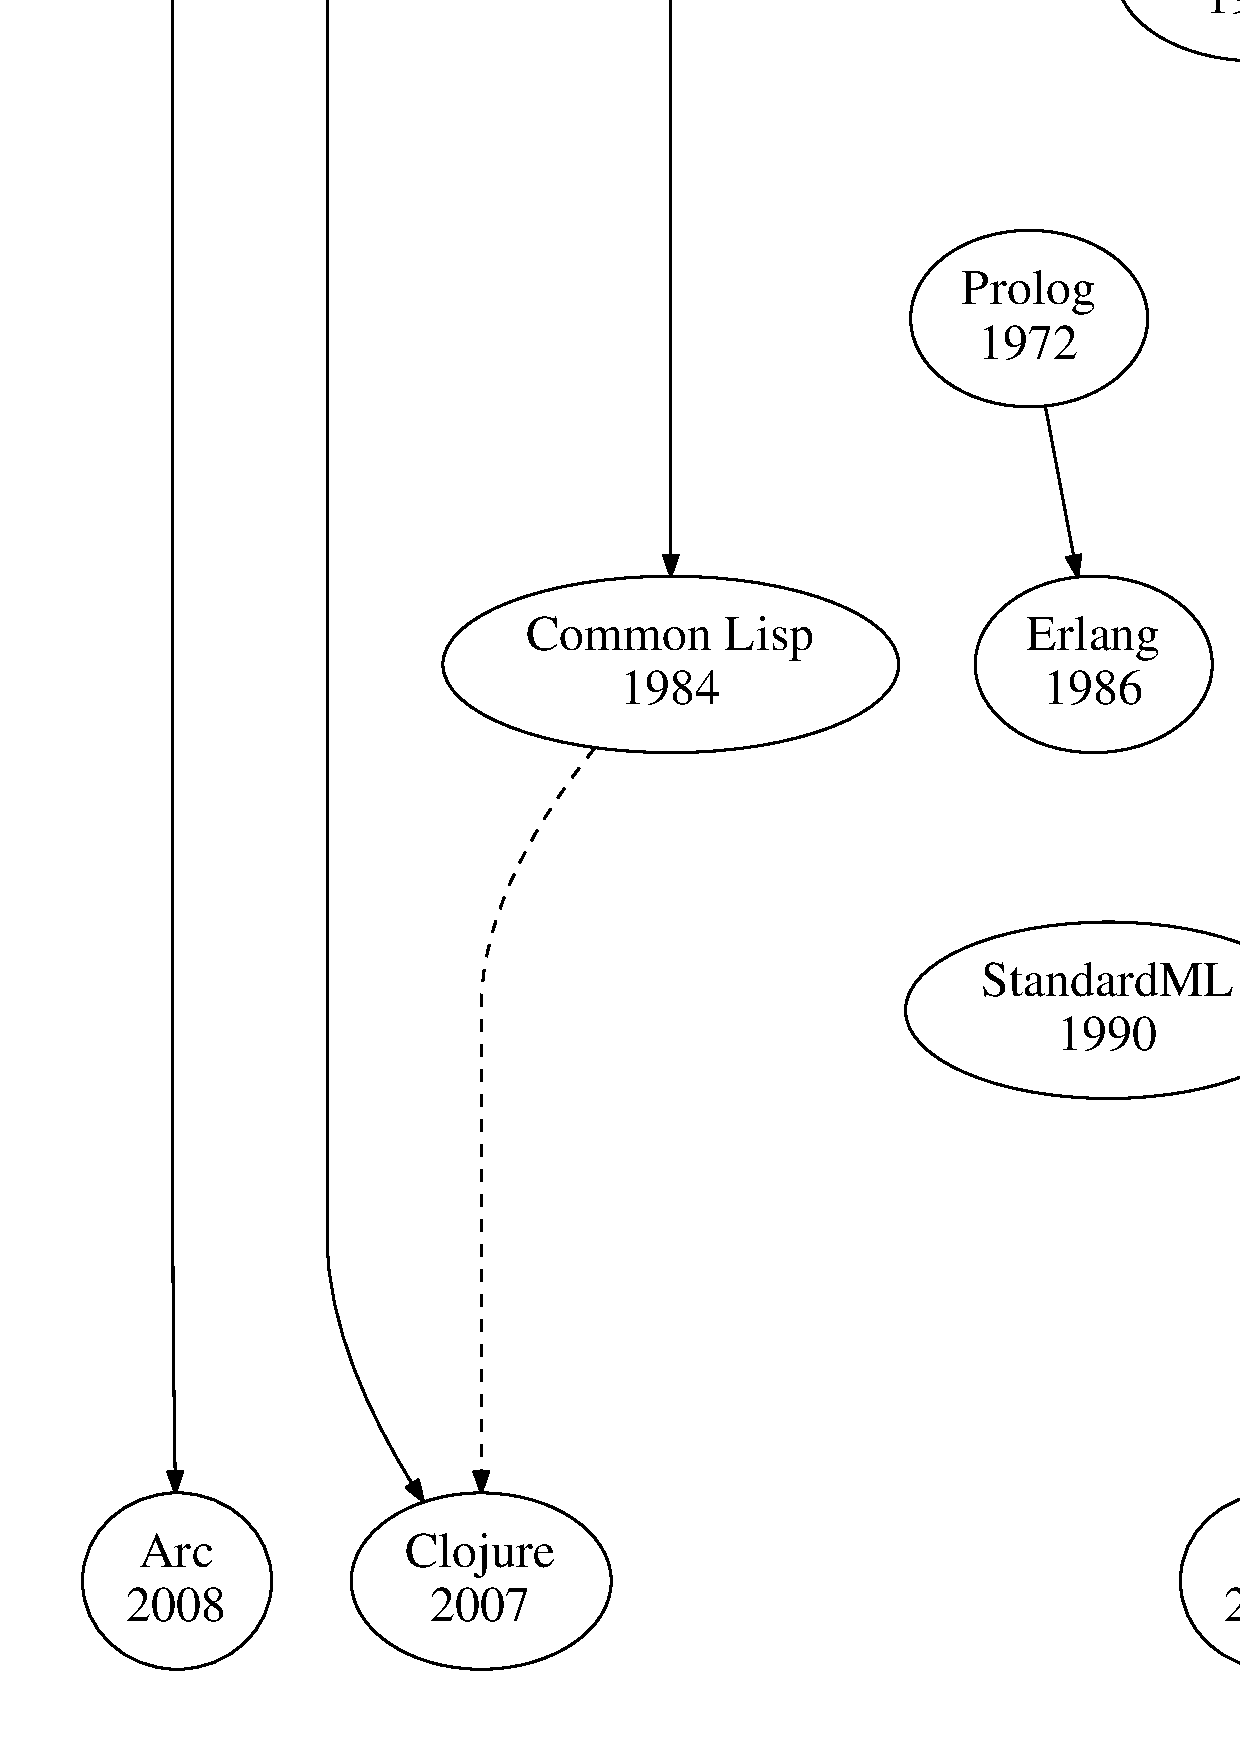
\includegraphics[width=\textwidth]{languages.pdf}
  \else
    \includegraphics[width=\textwidth]{languages.ps}
  \fi
\caption{Родословное древо функциональных языков}
\label{lineage}
\end{figure}

Как уже упоминалось в разделе \ref{benefits}, функциональные языки существуют довольно давно. Первый из них, Лисп, создан в 1958 году, всего на год позже первого императивного языка~--- Фортрана. Ещё один известный функциональный язык, РЕФАЛ, создан В.Ф.Турчиным в 1966 году. Но если РЕФАЛ стал широко известен довольно поздно (возможно, по причинам, далёким от программирования: он был создан в СССР в эпоху Холодной войны, а ФП развивалось в то время в основном по другую сторону Железного занавеса), то распространение Лиспа продолжалось всё время его существования. Уже в двухтысячных годах появились два новых популярных диалекта этого языка: Arc и Clojure.

Наиболее известные диалекты Лиспа~--- Common Lisp и Scheme. Первый чаще других вариантов Лиспа применяется на практике, а вторая используется в основном для обучения программированию. К сожалению, непоследовательная политика стандартизации сильно замедлила распространение Scheme как языка практического программирования.

Изучение Лиспа (скорее всего, Scheme) практически неизбежно для человека, интересущегося функциональным программированием, так как многие важные работы на эту тему используют именно Scheme в качестве языка примеров. Среди возможностей Scheme, отсутствующих в Эрланге, особенно интересны  продолжения (continuations)~--- способ сохранять как значение состояние программы в определённый момент.

Второй после Лиспа по влиятельности и многочисленности <<потомства>> функциональный язык это ML. В нём впервые была реализована очень мощная техника~--- {\em вывод типов}, то есть автоматическое определение компилятором типа выражения по контексту, в котором оно используется. Вывод типов избавляет программиста от целого класса неприятных ошибок. В этой книжке я использовал язык без вывода типов\footnote{На самом деле, похожие инструменты для Эрланга реализованы, но они гораздо слабее своих аналогов из языков-потомков ML.} только потому, что это сильно усложнило и удлинило бы курс.

Наиболее известные потомки ML это OCaml, F\# (построенный на базе OCaml язык для платформы .Net) и Haskell.

Именно Haskell считается <<передним краем>> исследований в области функционального программирования. В практическом программировании он применяется не так часто, возможно, потому, что его авторы очень жёстко отказываются вносить в язык полезные для индустрии, но <<некрасивые>> с точки зрения теории возможности~--- полушутливый девиз Haskell это <<Avoid success at all costs>> (<<Избегать успеха любой ценой>>). Пожалуй, Haskell~--- это второй после Scheme язык, изучения которого интересующемуся ФП человеку вряд ли удастся избежать. Изучить этот язык стоит хотя бы для того, чтобы познакомиться с такими интереснейшими концепциями, как ленивые вычисления или монады.

К сожалению, малопопулярен другой замечательный диалект ML~--- StandardML, очень красивый, гораздо более компактный, чем Haskell (и, на мой взгляд, более логичный синтаксически, чем OCaml и F\#) язык.

Ну и, наконец, не надо забывать, что Эрланг мы тоже изучили не до конца. Если вам понравился Эрланг, стоит всерьёз заняться изучением его возможностей. На самом деле, в этом курсе вообще не используется одно из главных преимуществ Эрланга~--- библиотека OTP, Open Telecom Platform, предоставляющая готовые решения для задач параллельного и распределённого программирования. <<За кадром>> остались также поведения (behaviours), обработка исключительных ситуаций, макросы и многое другое.

\section{Что ещё можно почитать про ФП}

Функциональному программированию посвящено довольно много книг, ресурсов в Интернете и журналов. Хорошей стартовой точкой для дальнейшего знакомства с миром ФП может стать журнал <<Практика функционального программирования>>, свободно доступный на сайте \url{http://fprog.ru/}. Кстати, в первом номере журнала опубликован обзор литературы по функциональному программированию, сделанный Алексеем Оттом~\cite{PFP_Ott}.

Ещё одна хорошая обзорная статья~--- <<Функциональное программирование для всех>> В.Ахмечета~\cite{Akhmechet}, опубликованная в журнале RSDN Magazine.

Среди книг прежде всего надо упомянуть <<Структуру и интерпретацию компьютерных программ>> Х.Абельсона и Дж.Сассмана~\cite{SICP}, которая по праву считается классической. Это учебник по программированию вообще, не только функциональному, но значительная часть материала изложена именно с помощью функциональных решений.

Большинство работ по алгоритмам и структурам данных расчитано на императивные языки. Эту ситуацию пытается исправить Крис Окасаки, автор книги <<Чисто функциональные структуры данных>>~\cite{Okasaki}. Ещё одна серьёзная работа по теоретическим аспектам программирования, ориентированная на ФП~--- <<Типы в языках программирования>> Б.Пирса~\cite{Pierce}.

Очень хороший пример практического программирования на функциональных языках приводится в статье Д.Астапова <<Давно не брал я в руки шашек>>~\cite{PFP_Astapov}. Интересующимся продвинутыми программистскими техниками будет, вероятно, интересно прочитать статьи А.Вознюка о продолжениях~\cite{PFP_Voznyuk} и И.Ключникова о суперкомпиляции~\cite{PFP_Klyuchnikov}. Впрочем, как уже говорилось, журнал <<Практика функционального программирования>>, в котором опубликованы все эти статьи, вообще рекомендуется к ознакомлению при наличии интереса к теме.

Замечательные учебники по языку Scheme и функциональному программированию~--- книги <<Little Schemer>>~\cite{little_schemer} и <<Seasoned Schemer>>~\cite{seasoned_schemer}, к сожалению, в отличие от SICP не переведены на русский язык.

Хороший вводный материал по языку Haskell~--- цикл статей Алексея Бешенова~\cite{Beshenov} и книга <<Изучай Haskell во имя добра!>>~\cite{Lipovacha}, а если говорить об источниках на английском языке~--- <<Real World Haskell>>~\cite{real_world_haskell}. По Стандартному ML на русском издана книга Р.Харпера <<Введение в Стандартный ML>>~\cite{Harper}.

Про возможности OTP, концепцию <<поведений>> (behaviours) можно прочитать в книге \cite{cesarini}. Из важных книг по Эрлангу, пока не переведённых на русский язык, надо упомянуть учебник Дж.Армстронга (создателя языка)~\cite{armstrong} и книгу <<Erlang and OTP in action>>~\cite{OTP_in_action}. Хороший вводный курс, правда, во многом дублирующий уже изложенное здесь~--- <<Learn You Some Erlang for Great Good>>~\cite{LYSE}.

\chapter*{Решения задач}
\addcontentsline{toc}{chapter}{Решения задач}
\markboth{Решения задач}{Азбука ФП}

\section*{Азбука ФП}
\addcontentsline{toc}{section}{Азбука ФП}

\solution{nand}

\lstinputlisting{abc/nand/logic.erl}

Вообще говоря, функцию \lstinline{nand} можно было бы определить гораздо проще:

\begin{lstlisting}
nand(true, true) -> false;
nand(_, _) -> true.
\end{lstlisting}

Но этот вариант функции \lstinline{nand} не будет выдавать ошибку, если передать ему в качестве аргументов что-то помимо атомов\index{Атом} \lstinline{true} и \lstinline{false}, что может затруднить поиск источника проблемы в неправильно написанной программе. Поэтому лучше перечислить все корректные варианты аргументов явно.

Помните, в Эрланге принят подход <<Let it fail>>~--- <<Пусть падает>>.

\solution{myor}

\lstinputlisting{abc/logic.erl}

\solution{author}

\lstinputlisting{abc/author.erl}

\solution{sign}

\lstinputlisting{abc/sign.erl}

\solution{divisor}

\lstinputlisting{abc/divisor.erl}

\solution{summ}

\lstinputlisting{abc/summ.erl}

\solution{divisors}

\lstinputlisting{abc/divisors.erl}

\solution{remainder}

\lstinputlisting{abc/remainder.erl}

\solution{number_sequence}

\lstinputlisting{abc/number_input.erl}

Эту задачу можно решить и иначе~--- например, вот так:

\lstinputlisting{abc/number_input/number_input.erl}

Идея решения та же самая, а как её оформить~--- вопрос вкуса. В таком варианте приодится дублировать оператор ввода, зато вместо \lstinline{case} используется сопоставление с образцом\index{Сопоставление с образцом}, что, по идее, должно делать код более понятным.

\solution{rember}

\lstinputlisting{abc/rember.erl}

\solution{listrev}

\lstinputlisting{abc/listrev.erl}

\solution{slice}

\lstinputlisting[language=erlang]{sugar/slice.erl}

\solution{flatten}

Алгоритм решения этой задачи можно коротко описать так: мы создаём временный список для хранения текущего разбираемого элемента (второй аргумент функции \lstinline{flatten/2}). Поначалу он пуст (это тот второй аргумент, который передаёт функции \lstinline{flatten/2} функция \lstinline{flatten/1}).

Если исходный список тоже пуст, то работа закончена (первый вариант функции).

Если исходный список не пуст, то мы берём его голову и помещаем во временный список для разбора (второе тело функции).

Если текущий разбираемый элемент это тоже список, то мы берём его голову, а хвост возвращаем в исходный список, где он будет дожидаться своей очереди (третье тело функции).

Наконец, если ни одно из предыдущих сопоставлений с образцом\index{Сопоставление с образцом} не увенчалось успехом, надо полагать, что хранилище разбираемых элементов не пусто (иначе бы сработали бы образцы 1 или 2) и то, что в нём лежит~--- не список (иначе сработал бы образец 3). Следовательно, это одиночное значение и мы можем смело помещать его в голову итогового списка.

\lstinputlisting{abc/flatten.erl}

\solution{palindrome}

\lstinputlisting[language=erlang]{best_practices/palindrome.erl}

\solution{perfect}
Функция \lstinline{divisors}, составляющая список делителей числа $N$, лежащих в интервале от 1 до $M$ включительно~--- это попросту индуктивное определение такого списка: если он заканчивается единицей, то только единица в него и войдёт, а если он должен состоять из чисел в интервале от единицы до некоего числа $M$, большего, чем единица, то в него войдут делители числа $N$ в интервале от 1 до $M-1$, а также само $M$, если оно тоже является делителем $N$.

Случай с единицей мы обрабатываем в \lstinline{divisors/1}, чтобы избежать лишнего вызова функции.

Функция \lstinline{lists:sum} из модуля \lstinline{lists}, подсчитывающая сумму списка чисел, ощутимо упрощает решение этой задачи.

Обратите внимание, что функция \lstinline{divisors} небезопасна и будет зацикливаться при значениях $M$ меньше 1. Здесь было разумным пожертвовать безопасностью в ущерб ясности; в реальных программах часто полезно делать наоборот.
\lstinputlisting[language=erlang]{abc/perfect.erl}
\pagebreak

\solution{brackets}
В этой задаче можно представлять строку для разбора либо как обычный эрланговский список, либо как битовую строку. Решение с битовыми строками чуть более громоздко, но в реальной жизни битовые строки гораздо полезнее <<строк>>, хранящихся как списки ASCII-кодов.

Алгоритм же в обоих решениях~--- один и тот же: сделаем стек, в который будем класть все открывающие скобки. Встречая закрывающую скобку, будем выпихивать со стека верхнее значение. Если тип закрывающей скобки из текущей позиции строки и открывающей скобки с вершины стека не совпали (или стек пуст), порядок скобок неправильный. Если после того, как вся строка разобрана, в стеке что-то осталось, порядок скобок тоже неправильный. Если же нам удалось подойти к концу строки с пустым стеком (или строка просто пустая), значит, порядок скобок~--- правильный.

\begin{figure}[!t,bracketspic]
\centerline{
\begin{pspicture}%[showgrid=true]
(10, 11)
\rput(2, 10.5){Входной список}
\rput(6.8, 10.5) {Стек}
\rput(0, 9){
  % Входной список
  \psgrid[gridlabels=0.0pt,subgriddiv=1](0,0)(0,0)(5,1)
  \rput(0.5, 0.5){[}
  \rput(1.5, 0.5){(}
  \rput(2.5, 0.5){<}
  \rput(3.5, 0.5){)}
  \rput(4.5, 0.5){]}
  % Операция
  \psbezier{->}(0.5,0)(0.5,-1)(6.5,0)(6.5,-1)
}
\rput(0, 7) {
  % Входной список
  \psgrid[gridlabels=0.0pt,subgriddiv=1](0,0)(0,0)(4,1)
  \rput(0.5, 0.5){(}
  \rput(1.5, 0.5){<}
  \rput(2.5, 0.5){)}
  \rput(3.5, 0.5){]}
  % Операция
  \psbezier{->}(0.5,0)(0.5,-1)(6.5,0)(6.5,-1)
  % Стек
  \psgrid[gridlabels=0.0pt,subgriddiv=1](0,0)(6,0)(7,1)
  \rput(6.5, 0.5){(}
}
\rput(0, 5) {
  % Входной список
  \psgrid[gridlabels=0.0pt,subgriddiv=1](0,0)(0,0)(3,1)
  \rput(0.5, 0.5){<}
  \rput(1.5, 0.5){)}
  \rput(2.5, 0.5){]}
  % Операция
  \psbezier{->}(0.5,0)(0.5,-1)(6.5,0)(6.5,-1)
  % Стек
  \psgrid[gridlabels=0.0pt,subgriddiv=1](0,0)(6,0)(8,1)
  \rput(6.5, 0.5){(}
  \rput(7.5, 0.5){[}
}
\rput(0, 3) {
  % Входной список
  \psgrid[gridlabels=0.0pt,subgriddiv=1](0,0)(0,0)(2,1)
  \rput(0.5, 0.5){)}
  \rput(1.5, 0.5){]}
  % Операция
  \psbezier{->}(0.5,0.0)(0.5,-1)(0.5,-1)(3.5,-1)
  \psbezier{->}(6.5,0.0)(6.5,-1)(6.5,-1)(4.5,-1)
  \rput(4, -1){\pscirclebox{?}}
  \psline{->}(4,-1.5)(4,-2)
  % Стек
  \psgrid[gridlabels=0.0pt,subgriddiv=1](0,0)(6,0)(9,1)
  \rput(6.5, 0.5){<}
  \rput(7.5, 0.5){(}
  \rput(8.5, 0.5){[}
  % Возвращаемое значение
  \rput(4, -2.5){false}
  \psbezier{->}(4.75,-2.5)(5.5,-3)(5.5,-2)(6.25,-2.5)
  \rput(7, -2.5){false}
}
\end{pspicture}
}
\caption{Функция \lstinline{is_valid_string/2} проверяет скобочную структуру <<[(<)]>> на правильность. Слева~--- входной список (первый аргумент функции), справа~--- стек (второй аргумент функции).}
\label{bracketspic}
\end{figure}

\lstinputlisting[language=erlang]{abc/brackets_str.erl}
\pagebreak
\lstinputlisting[language=erlang]{abc/brackets.erl}
\pagebreak

\solution{queue}

Идея решения вот в чём: реализуем очередь как два списка, входной и выходной. При помещении значения в очередь будем добавлять его в голову входного списка. При извлечении значения из очереди проверим, пуст ли выходной список. Если да, проверим, пуст ли входной. Если пуст и он, очередь пуста (второй вариант тела функции). А если входной список не пуст, развернём его, отдадим голову получившегося списка как выходное значение, а хвост поместим в выходной список (входной список, соответственно, становится пустым). Эти действия описаны в первом варианте тела функции. Ну а если выходной список не пуст, просто отдаём его голову, т.к. значения в нём уже стоят в правильном порядке (третий вариант тела функции).

Работа с организованной таким образом очередью будет выглядеть примерно так.

\begin{figure}[!t,queuepic]
\centerline{
\begin{pspicture}%[showgrid=true]
(9, 21)
\rput(3.0, 20.5){Входной}
\rput(3.0, 19.5){список}
\rput(6.0, 20.5){Выходной}
\rput(6.0, 19.5){список}
\rput(0, 18) {
  \psframe[linestyle=dotted](1.8,-0.2)(7.2, 1.2)
  % Операция
  \rput(0.5, 0.5){1}
  \psline{->}(0.8, 0.5)(1.6, 0.5)
}
\rput(0, 16) {
  \psframe[linestyle=dotted](1.8,-0.2)(7.2, 1.2)
  % Входной список
  \psgrid[gridlabels=0.0pt,subgriddiv=1](0,0)(2,0)(3,1)
  \rput(2.5, 0.5){1}
  % Операция
  \rput(0.5, 0.5){2}
  \psline{->}(0.8, 0.5)(1.6, 0.5)
}
\rput(0, 14) {
  \psframe[linestyle=dotted](1.8,-0.2)(7.2, 1.2)
  % Входной список
  \psgrid[gridlabels=0.0pt,subgriddiv=1](0,0)(2,0)(4,1)
  \rput(2.5, 0.5){2}
  \rput(3.5, 0.5){1}
  % Операция
  \rput(0.5, 0.5){3}
  \psline{->}(0.8, 0.5)(1.6, 0.5)
}
\rput(0, 12) {
  \psframe[linestyle=dotted](1.8,-0.2)(7.2, 1.2)
  % Операция
  \rput(8.5, 0.5){1}
  \psline{->}(7.4, 0.5)(8.2, 0.5)
  % Выходной список
  \psgrid[gridlabels=0.0pt,subgriddiv=1](0,0)(5,0)(7,1)
  \rput(5.5, 0.5){3}
  \rput(6.5, 0.5){2}
}
\rput(0, 10) {
  \psframe[linestyle=dotted](1.8,-0.2)(7.2, 1.2)
  % Операция
  \rput(0.5, 0.5){4}
  \psline{->}(0.8, 0.5)(1.6, 0.5)
  % Выходной список
  \psgrid[gridlabels=0.0pt,subgriddiv=1](0,0)(5,0)(7,1)
  \rput(5.5, 0.5){3}
  \rput(6.5, 0.5){2}
}
\rput(0, 8) {
  \psframe[linestyle=dotted](1.8,-0.2)(7.2, 1.2)
  % Входной список
  \psgrid[gridlabels=0.0pt,subgriddiv=1](0,0)(2,0)(3,1)
  \rput(2.5, 0.5){4}
  % Операция
  \rput(0.5, 0.5){5}
  \psline{->}(0.8, 0.5)(1.6, 0.5)
  % Выходной список
  \psgrid[gridlabels=0.0pt,subgriddiv=1](0,0)(5,0)(7,1)
  \rput(5.5, 0.5){3}
  \rput(6.5, 0.5){2}
}
\rput(0, 6) {
  \psframe[linestyle=dotted](1.8,-0.2)(7.2, 1.2)
  % Входной список
  \psgrid[gridlabels=0.0pt,subgriddiv=1](0,0)(2,0)(4,1)
  \rput(2.5, 0.5){5}
  \rput(3.5, 0.5){4}
  % Операция
  \rput(8.5, 0.5){2}
  \psline{->}(7.4, 0.5)(8.2, 0.5)
  % Выходной список
  \psgrid[gridlabels=0.0pt,subgriddiv=1](0,0)(6,0)(7,1)
  \rput(6.5, 0.5){3}
}
\rput(0, 4) {
  \psframe[linestyle=dotted](1.8,-0.2)(7.2, 1.2)
  % Входной список
  \psgrid[gridlabels=0.0pt,subgriddiv=1](0,0)(2,0)(4,1)
  \rput(2.5, 0.5){5}
  \rput(3.5, 0.5){4}
  % Операция
  \rput(8.5, 0.5){3}
  \psline{->}(7.4, 0.5)(8.2, 0.5)
}
\rput(0, 2) {
  \psframe[linestyle=dotted](1.8,-0.2)(7.2, 1.2)
  % Операция
  \rput(8.5, 0.5){4}
  \psline{->}(7.4, 0.5)(8.2, 0.5)
  % Выходной список
  \psgrid[gridlabels=0.0pt,subgriddiv=1](0,0)(6,0)(7,1)
  \rput(6.5, 0.5){5}
}
\rput(0, 0) {
  \psframe[linestyle=dotted](1.8,-0.2)(7.2, 1.2)
  % Операция
  \rput(8.5, 0.5){5}
  \psline{->}(7.4, 0.5)(8.2, 0.5)
}
\end{pspicture}
}
\caption{Организация очереди из двух списков.}
\label{queuepic}
\end{figure}

Компилируем модуль, загружаем определение записи:
\erlshell{c(listqueue).}{\{ok,listqueue\}}
\erlshell{rr("queue.hrl").}{{[}queue{]}}

Создаём новую очередь:
\erlshell{Q1 = \#queue\{\}.}{\#queue\{in = [],out = []\}}

Помещаем в очередь значение 1:
\erlshell{Q2 = listqueue:enqueue(Q1, 1).}{\#queue\{in = [1],out = []\}}

Помещаем в очередь значение 2:
\erlshell{Q3 = listqueue:enqueue(Q2, 2).}{\#queue\{in = [2,1],out = []\}}

Помещаем в очередь значение 3:
\erlshell{Q4 = listqueue:enqueue(Q3, 3).}{\#queue\{in = [3,2,1],out = []\}}

Извлекаем из очереди первое значение (1)~--- в этот момент входной список будет развёрнут и перемещён в выходной:
\erlshell{\{ok, Out1, Q5\} = listqueue:dequeue(Q4).}{\{ok,1,\#queue\{in = [],out = [2,3]\}\}}
\erlshell{Out1.}{1}

Добавляем в очередь значение 4 (с этого момента формируется новый входной список):
\erlshell{Q6 = listqueue:enqueue(Q5, 4).}{\#queue\{in = [4],out = [2,3]\}}

Добавляем в очередь значение 5:
\erlshell{Q7 = listqueue:enqueue(Q6, 5).}{\#queue\{in = [5,4],out = [2,3]\}}

Извлекаем из очереди второе значение (2):
\erlshell{\{ok, Out2, Q8\} = listqueue:dequeue(Q7).}{\{ok,2,\#queue\{in = [5,4],out = [3]\}\}}

Извлекаем из очереди третье значение (3):
\erlshell{\{ok, Out3, Q9\} = listqueue:dequeue(Q8).}{\{ok,3,\#queue\{in = [5,4],out = []\}\}}

Извлекаем из очереди четвёртое значение (4)~--- выходной список пуст, снова разворачиваем входной список и перемещаем его на место опустевшего выходного:
\erlshell{\{ok, Out4, Q10\} = listqueue:dequeue(Q9).}{\{ok,4,\#queue\{in = [],out = [5]\}\}}

Извлекаем из очереди пятое значение (5):
\erlshell{\{ok, Out5, Q11\} = listqueue:dequeue(Q10).}{\{ok,5,\#queue\{in = [],out = []\}\}}

Очередь пуста, при попытке извлечения дальнейших значений будет возвращена информация об ошибке:
\erlshell{listqueue:dequeue(Q11).}{\{error,"Queue is empty"\}}

Несмотря на наличие в этом алгоритме <<тяжёлой>> операции разворачивания списка, требующей $N$ шагов для списка из $N$ элементов, условиям задачи он отвечает, т.к. каждый проходящий через очередь элемент участвует в этой операции только один раз.

\lstinputlisting[language=erlang]{abc/listqueue.erl}

\solution{node_cut}

Обратите внимание на то, как функции \lstinline{trim/2} и \lstinline{trim/3} рекурсивно вызывают друг друга. Это полезный приём, который позволяет упростить отладку и тестирование, а также улучшить читаемость кода за счёт избавления от громоздких операторов ветвления.

\lstinputlisting[language=erlang]{abc/trimtree.erl}

\solution{node_count}

\lstinputlisting[language=erlang]{abc/treemeter.erl}

\section*{Полезные приёмы}
\addcontentsline{toc}{section}{Полезные приёмы}
\markright{Полезные приёмы}

\solution{already}

Хвостовая рекурсия уже используется в решениях задач \ref{summ}, \ref{divisors}, \ref{remainder}, \ref{listrev}, \ref{brackets}.

\solution{tail}

Функцию \lstinline{rember/2} из задачи \ref{rember} можно переписать следующим образом:

\lstinputlisting[language=erlang]{abc/tailrember.erl}

Проблема в том, что такой способ обработки списка разворачивает его, и нам приходится вызывать \lstinline{lists:reverse}, чтобы вернуть исходный порядок следования элементов. Поэтому применение здесь хвостовой рекурсии не очень оправдано. В решениях других задач применение хвостовой рекурсии принесёт ещё больше сложностей.

Не надо применять хвостовую рекурсию по любому поводу. Во-первых, она не всегда эффективнее обычной, во-вторых, помните: сначала стабильная работа программы, потом оптимизация.

\solution{perfect_list}

\lstinputlisting[language=erlang]{best_practices/perfect.erl}
\pagebreak

\solution{maptree}

\lstinputlisting[language=erlang]{best_practices/maptree.erl}

\solution{length}
\begin{lstlisting}
lists:foldl(fun(_, Length) -> Length + 1 end, 0, L).
\end{lstlisting}

\solution{foldrev}

\lstinputlisting[language=erlang]{best_practices/foldrev.erl}

\solution{mean}

\lstinputlisting[language=erlang]{best_practices/mean.erl}

\solution{foldl1}

\lstinputlisting[language=erlang]{best_practices/mylists.erl}

\solution{foldseq}

\lstinputlisting[language=erlang]{best_practices/myseq.erl}

\solution{ismemberof}

\lstinputlisting[language=erlang]{best_practices/ismemberof.erl}

\section*{Приятные мелочи}
\addcontentsline{toc}{section}{Приятные мелочи}
\markright{Приятные мелочи}

\solution{short_perfect}

\lstinputlisting[language=erlang]{sugar/perfect.erl}

\solution{common}

\lstinputlisting[language=erlang]{sugar/common_members.erl}

\solution{multiplication}

\lstinputlisting[language=erlang]{best_practices/multiplication.erl}

\solution{common_without_member}

\lstinputlisting[language=erlang]{sugar/common2.erl}

\solution{queens}

\lstinputlisting[language=erlang]{sugar/queens.erl}

%% Решение из статьи про задачу в Википедии %% (http://ru.wikipedia.org/wiki/%D0%97%D0%B0%D0%B4%D0%B0%D1%87%D0%B0_%D0%BE_%D0%B2%D0%BE%D1%81%D1%8C%D0%BC%D0%B8_%D1%84%D0%B5%D1%80%D0%B7%D1%8F%D1%85#.D0.A0.D0.B5.D0.B0.D0.BB.D0.B8.D0.B7.D0.B0.D1.86.D0.B8.D1.8F_.D0.BD.D0.B0_Erlang):

%% pmut([])->
%%         [[]];
%% pmut(A) ->
%%         [[H|T] || H <- A, T <- pmut(A--[H])].
 
%% start() ->
%%         N = 8, % size of board / num of queens (N>=4)
%%         ListP = pmut(lists:seq(1,N)),
%%         [Q || Q <- ListP, length(lists:usort([lists:nth(X,Q)+X || X <- %% Q])) == N, 
%%         length(lists:usort([lists:nth(X,Q)-X || X <- Q])) == N]

\solution{foldrrev}

\lstinputlisting[language=erlang]{sugar/foldrrev.erl}

\solution{linearize}

\lstinputlisting[language=erlang]{sugar/trees-linearize/trees.erl}

\solution{hanoi}

Сформулируем принципы перекладывания стопки из $N$ дисков.

Базовый случай в этой задаче~--- $N=0$, т.е. ситуация, когда нам ничего перекладывать не нужно. Большее количество дисков перекладывается по следующему алгоритму (стержень, с которого перемещаем диски, будем называть исходным, стержень, на который перемещаем диски~--- целевым, а третий~--- вспомогательным):

\begin{enumerate}
\item Взять $N-1$ дисков и переместить их с исходного стержня на вспомогательный.
\item Переместить оставшийся на исходном стержне диск на целевой стержень.
\item Переместить $N-1$ дисков со вспомогательного стержня на целевой.
\end{enumerate}

Первый и третий шаги предполагают перекладывание стопки дисков, то есть рекурсивный вызов процедуры перекладывания. Но так как в каждом следующем вызове $N$ гарантированно уменьшается, мы можем быть уверены, что рано или поздно рекурсия закончится.

\lstinputlisting[language=erlang]{sugar/hanoi.erl}

\solution{dropwhile}

Сложность с реализацией \lstinline{dropwhile} в том, что реакция на элемент, для которого переданная функция возвращает \lstinline{true}, должна отличаться в зависимости от того, встретился ли нам уже элемент, для которого эта функция вернула \lstinline{false}. Так как мы имеем дело со свёрткой\index{Свёртка списка}, мы не можем ввести какой-то дополнительный параметр, указывающий, так ли это~--- ведь тогда свёртка вернёт его вместе с итоговым списком, а это не то, что нам нужно.

Но на самом деле при левой свёртке\index{Свёртка списка!левая} таким параметром является сам итоговый список: если он пуст, значит, не отвечающий критерию элемент нам ещё не встречался и мы должны проверить текущий элемент с помощью функции-аргумента. Если список не пуст, мы должны безо всяких проверок поместить в него текущий элемент.

\lstinputlisting[language=erlang]{best_practices/dropwhile.erl}

Реализовать \lstinline{dropwhile} с помощью правой свёртки\index{Свёртка списка!правая}, строго говоря, невозможно~--- правая свёртка начинается с конца списка, что не позволяет нам найти первое с начала списка вхождение элемента с её помощью. Но динамическая типизация Эрланга позволяет нам реализовать обходное решение, жульническое по сути (реальная работа делается вне свёртки), но позволяющее <<обмануть>> функцию \lstinline{foldr}, подсунув ей функцию, которая формально удовлетворяет условиям задачи:

\lstinputlisting[language=erlang]{best_practices/rdropwhile.erl}

Идея этого решения в следующем: мы заранее находим первый элемент в списке, для которого функция \lstinline{F} вернёт \lstinline{false} и запоминаем его позицию (далее будем называть её <<линией отреза>>. После этого мы определяем функцию \lstinline{Trim}, у которой есть два варианта списка аргументов: либо текущий элемент списка и кортеж вида {\em \{Накопленный хвост списка, Позиция текущего элемента, Линия отреза\}}, либо текущий элемент и список.

\lstinline{Trim} будет добавлять к накопленному хвосту списка элемент за элементом, пока позиция текущего элемента не совпадёт с линией отреза. В этот момент она оставит в аргументе-накопителе только список. Следующие вызовы, обнаружив во втором аргументе список вместо кортежа, просто передадут аргумент-накопитель дальше.

Обратите внимание, что ситуация, когда элемент, для которого \lstinline{F} возвращает \lstinline{false}, так и не был найден, требует особой обработки.

Надо ещё раз подчеркнуть, что это решение является хаком в самом плохом смысле этого слова и непереносимо на многие функциональные языки с более строгим контролем типов, вроде Стандартного ML и Haskell (решения, построенные на аналогичной идее, пожалуй, возможны и там, но ценой ещё более уродливых ухищрений).

\solution{permutations}

Идея решения этой задачи вот в чём. В список перестановок списка длины $1$ входит единственный элемент~--- он сам. А перестановки списка большей длины можно получить так: по очереди удалять из списка каждый элемент, получать все перестановки оставшихся и в начало каждой из них подставлять удалённый элемент.

% Я видел где-то лучшее решение с --

\lstinputlisting[language=erlang]{sugar/permutations.erl}

\section*{От функционального программирования к параллельному}
\addcontentsline{toc}{section}{От функционального программирования к параллельному}
\markright{От ФП к ПП}

\solution{approximation}

\lstinputlisting[language=erlang]{parallel/montecarlo.erl}

\solution{fibmem}

\lstinputlisting[language=erlang]{parallel/fibmem.erl}

% Приложение: отладчик, запускающийся по debugger:start()? Трассировщик, если он может быть чем-то полезен? EUnit?

% Приложение: установка Эрланга на разных платформах?

\addcontentsline{toc}{chapter}{Литература}
\begin{thebibliography}{99}
\bibitem[Абельсон 2010]{SICP}
Абельсон Х., Сассман Дж. Дж. Структура и интерпретация компьютерных программ. М.: <<Добросвет>>, <<КДУ>>, 2010.
\bibitem[Астапов 2009]{PFP_Astapov}
Астапов Д. Давно не брал я в руки шашек // Практика функционального программирования, №1, 2009.
\bibitem[Ахмечет 2006]{Akhmechet}
Ахмечет В. Функциональное программирование для всех. // RSDN Magazine, №2, 2006.
\bibitem[Бешенов 2010]{Beshenov}
Бешенов А. Функциональное программирование на Haskell.\\
\href{http://www.ibm.com/developerworks/ru/library/l-haskell/}{Часть 1. Введение.}\\
\href{http://www.ibm.com/developerworks/ru/library/l-haskell2/}{Часть 2.Основные типы и классы.}\\
\href{http://www.ibm.com/developerworks/ru/library/l-haskell3/}{Часть 3. Определение функций.}\\
\href{http://www.ibm.com/developerworks/ru/library/l-haskell4/}{Часть 4. Свертки списков.}
\bibitem[Вознюк 2011]{PFP_Voznyuk}
Вознюк А. Продолжения в практике. // Практика функционального программирования, №7, 2011.
\bibitem[Златопольский 2007]{zlatopolsky}
Златопольский Д.М. Программирование: типовые задачи, алгоритмы, методы. М., 2007.
\bibitem[Ключников 2011]{PFP_Klyuchnikov}
Ключников И. Суперкомпиляция: идеи и методы. // Практика функционального программирования, №7, 2011.
\bibitem[Липовача 2012]{Lipovacha}
Липовача М. Изучай Haskell во имя добра! М.: <<ДМК Пресс>>, 2012.
\bibitem[Отт 2009]{PFP_Ott}
Отт А. Обзор литературы о функциональном программировании. // Практика функционального программирования, №1, 2009.
\bibitem[Пирс 2012]{Pierce}
Пирс Б., Типы в языках программирования. М.: <<Лямбда пресс>>, <<Добросвет>>, 2012.
\bibitem[Харпер 1996]{Harper}
Харпер Р. Введение в Стандартный ML. М., 1996.
\bibitem[Чезарини 2012]{cesarini}
Чезарини Ф., Томпсон С. Программирование в Эрланг. М.: <<ДМК Пресс>>,
2012.
\bibitem[Шень 2004]{shen}
Шень А. Программирование: теоремы и задачи. М.: МЦНМО, 2004.
\bibitem[99 problems]{99problems}
99 Problems на выбранном языке (точно есть для \href{http://www.haskell.org/haskellwiki/99_questions}{Haskell}, \href{http://aperiodic.net/phil/scala/s-99/}{Scala}, \href{https://sites.google.com/site/prologsite/prolog-problems}{Prolog}, \href{http://www.christiankissig.de/cms/index.php/en/programming/28-ocaml/28-99-problems-in-ocaml}{OCaml}, \href{http://www.informatimago.com/develop/lisp/l99/index.html}{Common Lisp}).
\bibitem[Armstrong 2007]{armstrong}
Armstrong J. Programming Erlang: Software for a Concurrent World. Pragmatic Bookshelf, 2007.
\bibitem[Friedman 1996]{little_schemer}
Friedman D.P., Fellsen M. The Little Schemer. MIT Press, 1996.
\bibitem[Friedman 1996,2]{seasoned_schemer}
Friedman D.P., Fellsen M. The Seasoned Schemer. MIT Press, 1996.
\bibitem[LYSE]{LYSE}
Learn You Some Erlang for Great Good, \url{http://learnyousomeerlang.com/}.
\bibitem[Logan 2011]{OTP_in_action}
Logan M., Merritt E., Carlsson R. Erlang and OTP in action. Manning Publications, 2011.
\bibitem[Miller]{miller}
Evan Miller. The Joy of Erlang; Or, How To Ride A Toruk, \url{http://www.evanmiller.org/joy-of-erlang.html}.
\bibitem[Okasaki 1999]{Okasaki}
Okasaki C. Purely Functional Data Structures. Cambridge University Press, 1999.
\bibitem[O'Sullivan 2008]{real_world_haskell}
O'Sullivan B., Goerzen J., D.B. Stewart. Real World Haskell. Code You Can Believe In. O'Reilly, 2008.
\end{thebibliography}

\appendix

\pagebreak
\addcontentsline{toc}{chapter}{Приложения}

\chapter{Краткий справочник по используемым функциям}

\section*{Ввод-вывод}
\addcontentsline{toc}{section}{Ввод-вывод}
\markright{Ввод-вывод}

Здесь приводятся только те функции, которые требуются для той или иной задачи. С полной документацией на упомянутые модули можно ознакомиться на сайте языка: \url{http://erlang.org/doc/}.

\begin{funcdescr}
\funcdoc{io:format/1}{Принимает строку с командами формата и выводит её на экран.}
\funcdoc{io:format/2}{Принимает строку с командами формата и список подставляемых значений; выводит на экран строку, в которую подставлены значения в соответствии с командами формата.}
\funcdoc{io:fread/2}{Принимает подсказку и строку формата; читает со стандартного ввода выражения и пытается привести их к типам, заданным строкой формата; в случае успеха возвращает кортеж из атома \lstinline{ok} и списка прочитанных значений, в случае  ошибки~--- кортеж из атома \lstinline{error} и описания ошибки.}
\funcdoc{io:read/1}{Принимает подсказку для ввода; читает со стандартного ввода выражение Эрланга и возвращает кортеж из атома \lstinline{ok} и прочитанного выражения в случае успеха либо кортеж из атома \lstinline{error} и описания ошибки в случае ошибки.}
\end{funcdescr}

\section*{Математика}
\addcontentsline{toc}{section}{Математика}
\markright{Математика}

\begin{funcdescr}
\funcdoc{abs/1}{Возвращает модуль числа.}
\funcdoc{math:sqrt/1}{Возвращает квадратный корень своего аргумента.}
\funcdoc{random:uniform/0}{Возвращает случайное вещественное число в интервале от 0.0 до 1.0.}
\funcdoc{random:uniform/1}{Возвращает случайное целое число в интервале от 1 до своего аргумента.}
\end{funcdescr}

\section*{Обработка списков}
\addcontentsline{toc}{section}{Обработка списков}
\markright{Обработка списков}

\begin{funcdescr}
\funcdoc{length/1}{Принимает список; возвращает длину этого списка.}
\funcdoc{lists:dropwhile/2}{Принимает функцию-тест и список; возвращает список, из которого выброшены все элементы до первого, для которого функция-тест вернула \lstinline{false}.}
\funcdoc{lists:filter/2}{Принимает функцию-тест и список; возвращает список, в котором оставлены только те элементы, для которых функция-тест вернула \lstinline{true}.}
\funcdoc{lists:foldl/3}{Левая свёртка: принимает функцию, начальное значение накопителя и список. Функция-аргумент должна принимать два параметра: текущее значение накопителя и текущий элемент списка, а возвращать новое значение накопителя. Применяет функцию-аргумент ко всем элементам списка слева направо (от первого до последнего). Возвращает итоговое значение накопителя.}
\funcdoc{lists:foldr/3}{Правая свёртка: принимает функцию, начальное значение накопителя и список. Функция-аргумент должна принимать два параметра: текущее значение накопителя и текущий элемент списка, а возвращать новое значение накопителя. Применяет функцию-аргумент ко всем элементам списка cправа налево (от последнего до первого). Возвращает итоговое значение накопителя.}
\funcdoc{lists:map/2}{Принимает функцию от одного аргумента и список; возвращает список результатов применения переданной функции к элементам списка.}
\funcdoc{lists:max/1}{Принимает список; возвращает самый большой элемент списка.}
\funcdoc{lists:member/2}{Принимает значение и список; возвращает \lstinline{true}, если значение содержится в списке, и \lstinline{false}, если нет.}
\funcdoc{lists:reverse/1}{Принимает список; возвращает список, элементы которого идут в обратном относительно исходного списка порядке.}
\funcdoc{lists:seq/2}{Принимает два целых числа; возвращает идущие подряд целые числа от первого до второго аргумента включительно.}
\funcdoc{lists:sort/1}{Принимает список; возвращает список с элементами исходного списка, отсортированными по возрастанию.}
\funcdoc{lists:sort/2}{Принимает функцию сравнения и список;   возвращает список, отсортированный по возрастанию в соответствии с функцией сравнения. Функция сравнения должна принимать два аргумента и возвращать \lstinline{true}, если первый аргумент меньше второго или равен ему, и \lstinline{false} в противном случае.}
\funcdoc{lists:sum/1}{Принимает список чисел; возвращает сумму его элементов.}
\end{funcdescr}

\section*{Структуры данных}
\addcontentsline{toc}{section}{Структуры данных}
\markright{Структуры данных}

\begin{funcdescr}
\funcdoc{dict:new/0}{Возвращает пустой словарь.}
\funcdoc{dict:append/3}{Принимает ключ, значение и словарь; возвращает новый словарь, в котором к значениям по переданному ключу добавилось переданное значение.}
\funcdoc{dict:find/2}{Принимает ключ и словарь. Если в словаре содержатся значения по этому ключу, возвращает кортеж \lstinline{\{ok, Values\}}, где \lstinline{Values}~--- список найденных значений; в противном случае возвращает атом \lstinline{error}.}
\end{funcdescr}

\section*{Служебные функции Эрланга}
\addcontentsline{toc}{section}{Служебные функции Эрланга}
\markright{Служебные функции Эрланга}

\begin{funcdescr}
\funcdoc{register/2}{Принимает атом и идентификатор процесса; если атом ещё не используется в качестве имени процесса, регистрирует процесс под этим именем и возвращает \lstinline{true}.}
\funcdoc{self/0}{Возвращает идентификатор процесса, из которого вызвана.}
\funcdoc{spawn/1}{Принимает функцию; запускает её в отдельном процессе и возвращает идентификатор этого процесса.}
\funcdoc{timer:tc/3}{Принимает имя модуля, имя функции и список аргументов; возвращает время в микросекундах, затраченное на вычисление переданной функции от переданных аргументов.}
\end{funcdescr}

\chapter{Команды формата}

\section*{Вывод}
\addcontentsline{toc}{section}{Вывод}
\markright{Вывод}

\renewcommand{\arraystretch}{1.5}
\begin{longtabu} to \linewidth {|X|X[2.8]|}
  \hline
  \lstinline{s} & Вывести строку.\\
  \hline
  \lstinline{w} & Вывести выражение Эрланга.\\
  \hline
  \lstinline{p} & Вывести выражение Эрланга с аккуратными переносами длинных строк и отступами. По умолчанию считает строку равной 80 символам. Принимает аргумент, задающий длину строки: так, команда формата <<{\tt \textasciitilde{}62p}>> будет считать длину строки равной 62 символам.\vspace{1ex}\\
  \hline
  \lstinline{B} & Вывести число в заданной системе счисления с основанием от 2 до 36, по умолчанию используется основание 10.\vspace{1ex}\\
  \hline
  \lstinline{n} & Перейти на новую строку.\\
  \hline
\end{longtabu}

\section*{Ввод}
\addcontentsline{toc}{section}{Ввод}
\markright{Ввод}

\begin{longtabu} to \linewidth {|X|X[2.8]|}
  \hline
  \lstinline{d} & Прочитать десятичное целое.\\
  \hline
  \lstinline{f} & Прочитать вещественное число.\\
  \hline
  \lstinline{s} & Прочитать строку. Принимает числовой аргумент~--- ограничение длины строки. Также принимает аргумент \lstinline{t}, включающий поддержку символов Unicode (нужно, если вы собираетесь вводить, например, русские буквы).\vspace{1ex}\\
  \hline
\end{longtabu}

Здесь приведены не все команды формата. Полное описание можно прочитать в документации модуля \lstinline{io} (\url{http://erlang.org/doc/man/io.html}).

% Предметный указатель
\pagebreak % Это хак, не знаю, как ещё его научить ставить правильную страницу.
\addcontentsline{toc}{chapter}{Предметный указатель}
\input{quicktour.ind}

\end{document}
%%% Local variables:
%%% eval: (auto-fill-mode -1)
%%% mode: latex
%%% mode: longlines
%%% coding: utf-8-unix
%%% End:


\end{document}
%%% Local variables:
%%% eval: (auto-fill-mode -1)
%%% mode: latex
%%% mode: longlines
%%% coding: utf-8-unix
%%% End:


\end{document}
%%% Local variables:
%%% eval: (auto-fill-mode -1)
%%% mode: latex
%%% mode: longlines
%%% coding: utf-8-unix
%%% End:


\end{document}
%%% Local variables:
%%% eval: (auto-fill-mode -1)
%%% mode: latex
%%% mode: longlines
%%% coding: utf-8-unix
%%% End:
